%%%%%%%%%%%%%%%%%%%%%%%%%%%%%%%%%%%%%%%%%
%%            LMU-Vorlage              %%
%%                                     %%
%%         zur Erstellung einer        %%
%%   Dissertation mit pdflatex/latex   %%
%%                                     %%
%%  (2002) Robert Dahlke               %%
%%         & Sigmund Stintzing         %%
%%%%%%%%%%%%%%%%%%%%%%%%%%%%%%%%%%%%%%%%%

\documentclass[12pt]{book}


%%%%%%%%%%%%%%%%%%%%%%%%%%%%
%%   Zusaetzliche Pakete  %%
%%%%%%%%%%%%%%%%%%%%%%%%%%%%

\usepackage{a4wide}
\usepackage{fancyhdr}
\usepackage{graphicx}
\usepackage{amsmath}
\usepackage{amssymb}
\usepackage{german}
\usepackage[bookmarks]{hyperref}


%%%%%%%%%%%%%%%%%%%%%%%%%%%%%%
%% Definition der Kopfzeile %%
%%%%%%%%%%%%%%%%%%%%%%%%%%%%%%

\pagestyle{fancyplain}
\renewcommand{\chaptermark}[1]%
         {\markboth{\thechapter.\ #1}{}}
\renewcommand{\sectionmark}[1]%
         {\markright{\thesection\ #1}}
\lhead[\fancyplain{}{\bfseries\thepage}]%
    {\fancyplain{}{\bfseries\rightmark}}
\rhead[\fancyplain{}{\bfseries\leftmark}]%
    {\fancyplain{}{\bfseries\thepage}}
\cfoot{}


%%%%%%%%%%%%%%%%%%%%%%%%%%%%%%%%%%%%%%%%%%%%%%%%%%%%%
%%  Definition des Deckblattes und der Titelseite  %%
%%%%%%%%%%%%%%%%%%%%%%%%%%%%%%%%%%%%%%%%%%%%%%%%%%%%%

\newcommand{\LMUTitle}[9]{
  \thispagestyle{empty}
  \vspace*{\stretch{1}}
  {\parindent0cm
   \rule{\linewidth}{.7ex}}
  \begin{flushright}

    \vspace*{\stretch{1}}
    \sffamily\bfseries\LARGE
    #1\\
    \large #9\\
    \vspace*{\stretch{1}}
    \sffamily\bfseries\large
    #2
    \vspace*{\stretch{1}}
  \end{flushright}
  \rule{\linewidth}{.7ex}
  \vspace*{\stretch{5}}
  \begin{center}
    
\includegraphics[width=2in]{siegel}
  \end{center}
  \vspace*{\stretch{1}}
  \begin{center}\sffamily\LARGE{#5}\end{center}
  \newpage
  \thispagestyle{empty}

  \cleardoublepage
  \thispagestyle{empty}

  \vspace*{\stretch{1}}
  {\parindent0cm
  \rule{\linewidth}{.7ex}}
  \begin{flushright}
    \vspace*{\stretch{1}}
    \sffamily\bfseries\LARGE
    #1\\
    \large #9\\
    \vspace*{\stretch{1}}
    \sffamily\bfseries\large
    #2
    \vspace*{\stretch{1}}
  \end{flushright}
  \rule{\linewidth}{.7ex}

  \vspace*{\stretch{3}}
  \begin{center}
    \Large Diplomarbeit\\
    \Large an der #4\\
    \Large der Ludwig--Maximilians--Universit"at\\
    \Large M\"unchen\\
    \vspace*{\stretch{1}}
    \Large vorgelegt von\\
    \Large #2\\
    \Large aus #3\\
    \vspace*{\stretch{2}}
    \Large M\"unchen, den #6
  \end{center}

  \newpage
  \thispagestyle{empty}

  \vspace*{\stretch{1}}

  \begin{flushleft}
    \large Erstgutachter:  #7 \\[1mm]
    \large Zweitgutachter: #8 \\[1mm]
  \end{flushleft}

  \cleardoublepage
}




%%%%%%%%%%%%%%%%%%%%%%%%%%%%
%%  Beginn des Dokuments  %%
%%%%%%%%%%%%%%%%%%%%%%%%%%%%

\begin{document}


  \frontmatter


  \LMUTitle
      {Stochastische Geometrie und Perkolation}
      {Richard Neher}                       % Vor- und Nachname des Autors
      {G\"ottingen}                             % Geburtsort des Autors
      {Fakult\"at f\"ur Physik}                         % Name der Fakultaet
      {M"unchen 2003}                          % Ort und Jahr der Erstellung
      {\today}                            % Tag der Abgabe
      {Prof. H. Wagner}                          % Name des Erstgutachters
      {Prof. H.-O. Georgii}                         % Name des Zweitgutachters
      {Die Rolle der Euler-Charakteristik}  %untertitel

  \tableofcontents
  \markboth{Inhaltsverzeichnis}{Inhaltsverzeichnis}


  \cleardoublepage

  \mainmatter\setcounter{page}{1}
  %10.9.03

\chapter{Einleitung}
Die Kenntnis der Perkolationsschwelle ist f\"ur die Vorhersage der Eigenschaften von Strukturen, die aus zuf\"allig angeordneten Objekten bestehen, sehr wichtig. Zwischen der mittleren Euler-Charakteristik solcher Strukturen und ihrer Perkolationsschwelle besteht ein enger Zusammenhang, und die mittlere Euler-Charakteristik k\"onnte daher zur Vorhersage von Perkolationsschwellen dienen. Dieser Zusammenhang wird in der vorliegenden Arbeit untersucht.
\\Zu Beginn dieses Kapitels werden Perkolationsprozesse an einigen Beispielen erl\"autert und Aspekte der Perkolationstheorie, die im weiteren Verlauf ben\"otigt werden, dargelegt. Anschlie"send wird der Befund, dass die Nullstelle der mittleren Euler-Charakteristik bei einigen Perkolationsproblemen in der N\"ahe der Perkolationsschwelle liegt, vorgestellt. Die Euler-Charakteristik wird im zweiten Kapitel ausf\"uhrlicher behandelt.
\section{Perkolation}
Um an einem Beispiel darzulegen, was man unter Perkolation versteht, betrachten wir ein leitendes Netzwerk, bestehend aus Knoten (Umspannwerke) und Verbindungen (Hochspannungsleitungen) \cite{Zallen:83}. Das Netzwerk k\"onnte zur Elektrizit\"atsversorgung eines Landes dienen. Der Einfachheit halber seien die Knoten auf einem Quadratgitter angeordnet, und jeder Knoten sei mit seinen vier Nachbarn verbunden. Eine Gruppe von Saboteuren will die Stromversorgung unterbrechen und beginnt die Verbindungen (Hochspannungsleitungen) zwischen den Knoten in zuf\"alliger Reihenfolge zu zerschneiden. Im Laufe ihrer T\"atigkeit wird Strom, der durch das Netzwerk von linken Rand zum rechten Rand flie"sen kann, immer kleiner und verschwindet, wenn exakt die H\"alfe aller Verbindungen durchtrennt ist. Das teilweise zerst\"orte Netzwerk und der Strom von linken zum rechten Rand als Funktion des Bruchteils $p$ der intakten Verbindungen sind in Abbildung \ref{fig:bondsabotage} skizziert. Anstatt die Verbindungen zwischen den Knoten zu zerst\"oren, k\"onnten die Saboteure auch die Knoten selbst angreifen. In diesem Fall gen\"ugt es, etwas mehr als 40\% der Stationen zu zerst\"oren, damit kein Strom mehr flie"st. Das Ergebnis dieses Sabotageaktes und der Strom in Abh\"angigkeit des Bruchteils der intakten Knoten sind in  Abbildung \ref{fig:sitesabotage} skizziert. Bei beiden Sabotageakten nimmt der Strom mit der Zahl der Zerst\"orungen ab und es existiert ein Wert $p=p_c$, unterhalb dessen der linke und rechte Rand nicht mehr verbunden sind, und daher kein Strom mehr flie"st. Den Wert $p_c$ nennt man Perkolationsschwelle. Bei $p=p_c$ \"andern sich globale Eigenschaften des Netzwerkes durch eine infinitesimale Variation von $p$, denn f\"ur $p>p_c$ existiert ein zusammenh\"angendes Netzwerk, das linken und rechten Rand verbindet, w\"ahrend es f\"ur $p<p_c$ nur isolierte Inseln gibt. 
\begin{figure}[tbp]
  \centering
  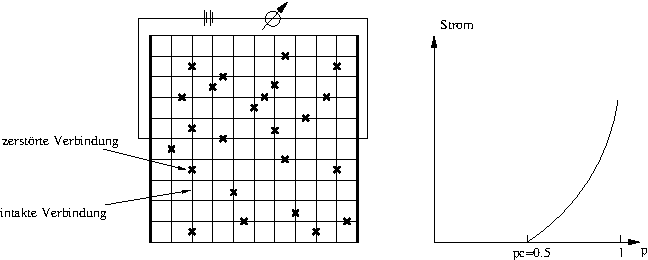
\includegraphics{./Einleitung-figs/sabobond}
  \caption{Zuf\"allige Zerst\"orung der Verbindungen eines leitenden Netzwerks: Rechts ist der Strom als Funktion des Bruchteils $p$ der intakten Verbindungen skizziert. Wenn weniger als 50\% der Verbindungen intakt sind, flie"st kein Strom mehr.}
  \label{fig:bondsabotage}
\end{figure}
\begin{figure}[bt]
  \centering
  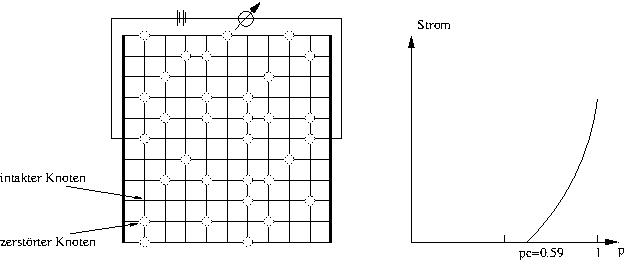
\includegraphics{./Einleitung-figs/sabosite}
  \caption{Zuf\"allige Zerst\"orung der Knoten eines leitenden Netzwerks: Rechts ist der Strom als Funktion des Bruchteils $p$ der intakten Knoten skizziert. Wenn weniger als 59\% der Knoten intakt sind, flie"st kein Strom mehr.}
  \label{fig:sitesabotage}
\end{figure}
Ein \"ahnliches Verhalten beobachtet man in Systemen, die einen thermischen Phasen\"ubergang zeigen. Dort existiert eine kritische Temperatur $T_c$, an der sich makroskopische Eigenschaften des Systems \"andern. F\"ur $T<T_c$ existieren langreichweitige Korrelationen zwischen den Konstituenten, w\"ahrend diese Korrelationen f\"ur $T>T_c$ exponentiell abfallen. 
\\Eine scharfe Perkolationsschwelle beobachtet man aber nur in einem unendlich gro"sen System. Ist das System endlich, ist die Wahrscheinlichkeit, dass eine Verbindung zwischen gegen\"uberliegenden R\"andern existiert, f\"ur kleine $p$ nahe null, w\"ahrend sie f\"ur gro"se $p$ fast eins ist. Der \"Ubergangsbereich wird mit wachsender Systemgr\"o"se immer schmaler. Im Limes unendlicher Systemgr\"o"se wird dieser \"Ubergang scharf, und die Wahrscheinlichkeit, dass beide Seiten verbunden sind, zu einer Stufenfunktion mit Sprung bei $p_c$. 
\\Die Sabotageakte sind Beispiele f\"ur die beiden am besten untersuchten Perkolationsprozesse auf Gittern. Die Knoten entsprechen den Vertices eines Gitters; die Verbindungen zwischen den Knoten sind die Gitterkanten zwischen den Vertices. Beim ersten Sabotageakt sind alle Vertices (Knoten) vorhanden, aber nur ein Teil $p$ der Gitterkanten ist besetzt (unzerst\"ort). Dieses Modell beschreibt \textbf{bond-Perkolation}. 
Im anderen Fall ist nur ein Teil der Knoten intakt, und man nennt Vertices, die intakten Knoten entsprechen, besetzt. Benachbarte, besetzte Vertices sind durch Gitterkanten verbunden. Dieses Modell beschreibt \textbf{site-Perkolation} und der Anteil der besetzten Vertices ist die Besetzungswahrscheinlichkeit $p$. Bond- und site-Perkolation sind in ihren mathematischen Aspekten sehr \"ahnlich. In der Tat l\"asst sich jedes bond-Perkolationsproblem als site-Perkolation auf dem \"Uberdeckungsgitter (engl.: covering lattice) formulieren. Das \"Uberdeckungsgitter entsteht, indem man auf jede Gitterkante (die bonds) einen Vertex setzt, und alle Vertices verbindet, deren zugeh\"orige Kanten an einem gemeinsamen Vertex enden (siehe Abb. \ref{fig:covering_einleit}). Die physikalische Interpretation von bond- und site-Perkolation ist aber durchaus unterschiedlich.
\begin{figure}[htbp]
  \centering
  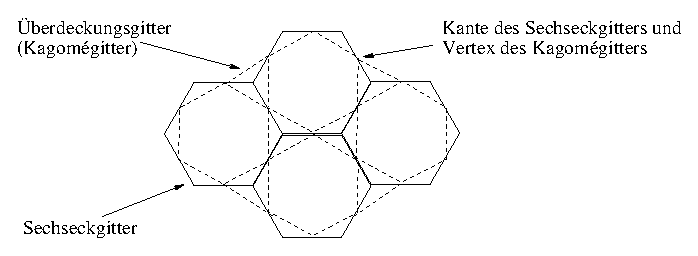
\includegraphics{./Einleitung-figs/cov}
  \caption{Das \"Uberdeckungsgitter des Sechseckgitters ist das Kagom\'egitter.}
  \label{fig:covering_einleit}
\end{figure}
\\Das bond-Perkolationsmodell wird z.B. verwendet, um den Prozess der Gelbildung zu beschreiben. Man betrachtet Monomere in einem Container und nimmt an, dass sie auf den Vertices eines Gitters angeordnet sind, und, dass sich zwischen diesen Monomeren mit einer gewissen Wahrscheinlichkeit $p$ chemische Bindungen ausbilden (siehe Abb. \ref{fig:gel}). Ist $p$ klein, existieren nur sehr wenige Bindungen, und die entstehenden Polymere sind klein. Mit $p$ wachsen die Molek\"ule. Bei $p=p_c$ entsteht erstmals ein gro"ses Makromolek\"ul, dass sich durch den ganzen Container erstreckt. Der Inhalt des Containers wird von einer Fl\"ussigkeit zu einem Gel. Das Makromolek\"ul enth\"alt aber nur einen Bruchteil der Molek\"ule und durchzieht den nach wie vor fl\"ussigen Anteil wie ein Netz. W\"achst $p$ weiter an, wird das Netz immer dichter, bis es schlie"slich bei $p=1$ alle Monomere enth\"alt.
\begin{figure}[tbp]
  \centering
  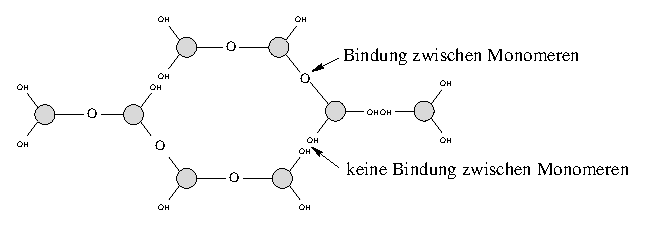
\includegraphics{./Einleitung-figs/gel}
  \caption{Monomere auf einem Sechseckgitter, zwischen denen sich chemische Bindungen ausbilden k\"onnen.}
  \label{fig:gel}
\end{figure}
\\Ein prominentes Beispiel f\"ur einen site-Perkolationsprozess ist die Modellierung von Waldbr\"anden. Die B\"aume im Wald werden durch Vertices eines zweidimensionalen Gitters dargestellt. Auf jedem Gitterplatz steht mit Wahrscheinlichkeit $p$ ein Baum, d.h. Vertices sind mit Wahrscheinlichkeit $p$ besetzt. Wenn in einen beliebigen Baum ein Blitz einschl\"agt, beginnt der Baum zu brennen. Der brennende Baum entz\"undet alle B\"aume in seiner Nachbarschaft und es entwickelt sich ein Waldbrand (siehe Abb. \ref{fig:waldbrand}). Die erwartete Anzahl $S$ der verbrannten B\"aume h\"angt von $p$ ab. Ist $p$ sehr klein, hat der Baum typischerweise keine Nachbarn und $S$ ist klein. Ist $p$ nahe eins, wird der Wald vollst\"andig verbrennen und $S$ ist unendlich. 
\begin{figure}[tbp]
  \centering
  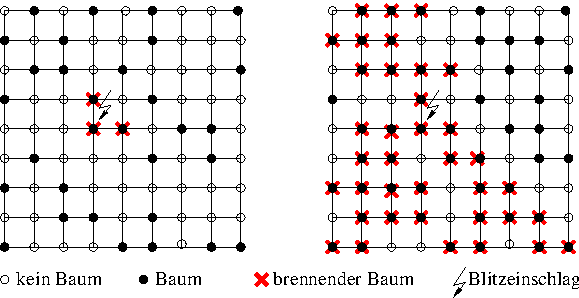
\includegraphics{./Einleitung-figs/waldbrand}
  \caption{Links: ein sp\"arlich bewachsener Wald, in dem sich der Brand nicht ausbreiten kann. Rechts: ein dicht bewachsener Wald mit gro"sr\"aumigen Brandschaden.}
  \label{fig:waldbrand}
\end{figure}
Bei $p=p_c$ \"andert sich das erwartete Schicksal des Waldes dramatisch. F\"ur $p<p_c$ existieren nur endliche zusammenh\"angende Bereiche, sog. Cluster, und der Waldbrand bleibt auf einen endlichen Cluster beschr\"ankt. Die erwartete Anzahl der verbrannten B\"aume $S$ ist die mittlere Clustergr\"o"se und f\"ur $p<p_c$ endlich. Die Wahrscheinlichkeit, dass ein Baum, der im Abstand $r$ vom Einschlagort des Blitzes steht, verbrennt, ist durch die  \textit{pair-connectedness} Funktion $\rho(r)$ gegeben. Die pair-connectedness Funktion ist die Wahrscheinlichkeit, dass zwei besetzte Vertices im Abstand $r$ zum gleichen Cluster geh\"oren. F\"ur $p<p_c$ und gro"se $r$ f\"allt $\rho$ mit $r$ exponentiell auf einer Skala $\xi(p)$ ab. F\"ur $p>p_c$ existiert ein unendlicher Cluster, und wenn der Blitz in einen Baum dieses Clusters einschl\"agt, bleibt der Waldbrand nicht auf ein endliches Gebiet beschr\"ankt. Die Wahrscheinlichkeit, dass ein Vertex zu einem unendlichen Cluster geh\"ort, wird Perkolationswahrscheinlichkeit genannt. F\"ur die Perkolationswahrscheinlichkeit gilt  
\begin{equation}
  P_{\infty}(p) \quad \begin{cases} =0 & p<p_c \\ >0 & p>p_c \end{cases}.
\end{equation}
F\"ur $p>p_c$ schl\"agt der Blitz also mit endlicher Wahrscheinlichkeit in einen Baum aus dem unendlichen Cluster ein, und $S$ ist unendlich. Die Wahrscheinlichkeit, dass zwei B\"aume zum gleichen Cluster geh\"oren, ist auch bei beliebig gro"sen Abstand echt gr\"o"ser null und es gilt $\rho(r) \rightarrow P_{\infty}(p)^2$ f\"ur $r\rightarrow \infty$. Schr\"ankt man die mittlere Clustergr\"o"se auf endliche Cluster ein, ist $S_{endl}(p)$ sowohl f\"ur $p<p_c$, als auch $p>p_c$ endlich, und divergiert f\"ur $p\rightarrow p_c$. Unterhalb von $p_c$ ist $S(p)=S_{endl}(p)$.\\
Der Wert der Perkolationsschwelle $p_c$ h\"angt von dem Gitter, auf dem die Vertices angeordnet sind, ab. Vertices der Gitter sind durch Gitterkanten verbunden, und in aller Regel gilt, dass $p_c$ umso kleiner ist, je mehr Nachbarn die Vertices haben. Im Dreiecksgitter z.B. hat ein Vertex sechs Nachbarn, w\"ahrend ein Vertex des Quadratgitters nur vier Nachbarn hat. Die site- und die bond-Perkolationsschwelle des Dreiecksgitters liegen unterhalb der entsprechenden Schwellen des Quadratgitters. W\"ahr\-end $p_c$ von Gitter zu Gitter variert, beobachtet man f\"ur andere Gr\"o"sen in der N\"ahe von $p_c$ universelles Verhalten (siehe Abb. \ref{fig:universal}). F\"ur diese Gr\"o"sen findet man  
\begin{eqnarray}
P_{\infty}(p) & \sim & (p-p_c)^\beta \quad \text{f\"ur} \quad p>p_c, \\
S_{endl}(p) & \sim & |p-p_c|^{-\gamma},  \\
\xi & \sim & |p-p_c|^{-\nu}  \quad \text{f\"ur} \quad p<p_c.
\end{eqnarray}
Die funktionelle Abh\"angigkeit dieser Gr\"o"sen von $p$ ist universell, und die Exponenten h\"angen nur von der Dimension des verwendeten Gitters ab. Das Skalenverhalten kann mit Renormierungsargumenten verstanden werden, ist aber nicht im mathematischen Sinne bewiesen.
\begin{figure}[tbp]
  \centering
  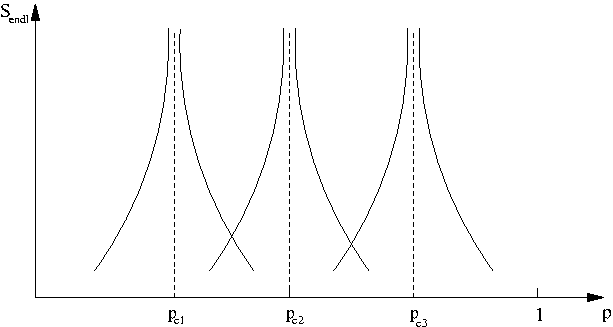
\includegraphics{./Einleitung-figs/universal}
  \caption{Schematische Darstellung des universellen asymptotischen Verhalten der mittleren Clustergr\"o"se endlicher Cluster $S_{endl}(p)$ von Perkolationsprozessen mit unterschiedlichem $p_c$.}
  \label{fig:universal}
\end{figure}
\\Der Perkolationsprozess ist in vielen Aspekten kontinuierlichen thermischen Phasen\"uber\-g\"an\-gen mit divergierender Korrelationsl\"ange sehr \"ahnlich. In der Tat geht der Phasen\"ubergang in Spinmodellen mit dem erstmaligen Auftreten eines unendlichen Spinclusters einher \cite{Coniglio:77}. Perkolation kann als Limes $\lambda \rightarrow 1$ des $\lambda$-Zustands-Pottsmodells erhalten werden (\cite{Fortuin:72}, siehe auch Abschnitt \ref{sec:matchingpoly}). $P_{\infty}(p)$ spielt die Rolle des Ordnungsparameters, die mittlere Clustergr\"o"se $S$ die der Suszeptibilit\"at und die charakteristische L\"ange der Pair-connectedness Funktion entspricht der Korrelationsl\"ange zweier Spins.\\
Perkolation wurde als Modell f\"ur ungeordnete por\"ose Medien eingef\"uhrt und hat im Laufe der Jahrzehnte in so unterschiedlichen Bereichen wie Epidemologie, der Theorie der Phasen\"uberg\"ange und der Beschreibung kosmischer Strukturen Anwendungen gefunden. F\"ur eine umfassende Einf\"uhrung in die mathematische Perkolationstheorie sei auf die B\"ucher von Grimmett \cite{Grimmett:99} und Hughes \cite{Hughes:96} verwiesen, f\"ur die physikalischen Aspekte der Perkolationstheorie ist das Buch von Stauffer und Aharony \cite{Stauffer:95} eine unterhaltsame Quelle.\\

Das Hauptaugenmerk der Perkolationstheorie liegt auf dem Verst\"andnis der universellen Eigenschaften in der N\"ahe des kritischen Punktes. F\"ur viele praktische Anwendungen ist aber die Kenntnis des Wertes von $p_c$ entscheidend. Die Art und Weise, wie $p_c$ von den mikroskopischen Details des Perkolationsprozesses, insbesondere der Gitterstruktur abh\"angt, ist Gegenstand dieser Arbeit. Klaus Mecke und Herbert Wagner haben bemerkt, dass die Nullstelle $p_0$ der mittleren Euler-Charakteristik bei einer Reihe von Perkolationsproblemen in der N\"ahe von $p_c$ liegt. Das Ziel der Arbeit ist es, diesen Befund ausf\"uhrlicher zu untersuchen, und $p_0$ als Sch\"atzwert f\"ur $p_c$ empirisch zu begr\"unden. Diese Faustregel ist vergleichbar mit dem Lindemann-Kriterium f\"ur das Schmelzen von Kristallen, welches besagt, dass ein Kristall schmilzt, sobald die mittlere Schwingungsamplitude der Kristall\-atome ungef\"ahr $1/10$ des Gitterabstandes erreicht. In vergleichbarer Weise ist die Nullstelle der Euler-Charakteristik geeignet den Perkolations\"ubergang abzusch\"atzen. In zwei Dimensionen ist die Euler-Charakteristik die Differenz der Zahl der Cluster und der Zahl der in diesen Clustern enthaltenen L\"ocher. Die Euler-Charakteristik wird negativ, wenn die L\"ocher \"uberwiegen. Unterhalb von $p_c$ besteht die Anordnung aus vielen endlichen Clustern, die L\"ocher enthalten k\"onnen. Oberhalb von $p_c$ exisitert ein unendlicher Cluster, der unbesetzte Inseln enth\"alt, die wiederum endliche besetzte Cluster enthalten k\"onnen. Oberhalb von $p_c$ ist also jeder endliche Cluster in einem Loch des unendlichen Clusters enthalten und jeder positive Beitrag zur Euler-Charakteristik geht mit einem negativen Beitrag einher. Man erwartet also f\"ur $p<p_c$ positive und f\"ur $p>p_c$ negative Euler-Charakteristik und es ist plausibel, dass $p_0$ in der N\"ahe von $p_c$ liegt. 

\subsection{Weitere Perkolationsmodelle}
Als anschauliche Beispiele f\"ur bond- und site-Perkolation haben wir Saboteure betrachtet, die in zuf\"alliger Reihenfolge entweder Verbindungen oder Knoten eines Netzwerkes zerst\"oren. Wenn zwei verschiedene Gruppen von Saboteuren, von denen eine Verbindungen und die andere Knoten zerst\"ort, gleichzeitig eine Attacke starten, erzeugen sie einen gemischten \textbf{bond-site-Perkolationsprozess}. Die Bruchteile der Verbindungen $p_b^*$ und Knoten $p_s^*$, die zum Zeitpunkt, an dem die Leitf\"ahigkeit verschwindet, zerst\"ort sind, h\"angen von den Geschwindigkeiten ab, mit denen Verbindungen bzw. Knoten zerst\"ort werden. Der kritische Ort ist eine Kurve $p_s^*(p_b^*)$ in der $(p_s,p_b)$-Ebene. Auch die anderen angef\"uhrten Beispiele lassen sich leicht auf bond-site-Perkolation verallgemeinern. Wenn beim Modell der Gelierung nur auf einem Bruchteil der Gitterpunkte ein Monomer sitzt, erh\"alt man einen bond-site-Perkolationsprozess. Entsprechend k\"onnten im Waldbrandmodell brennende B\"aume ihre Nachbarn nicht mit Sicherheit, sondern nur mit einer gewissen Wahrscheinlichkeit entz\"unden.\\
Perkolation auf Gittern ist ein einfaches Modell, das reale Ph\"anomene nur eingeschr\"ankt wiedergeben kann. Perkolation kann aber ebenso gut als kontinuierliches Modell formuliert werden. Man kann beispielsweise Punkte nach einen gewissen Zufallsprozess verteilen und sie nach einer geeigneten Vorschrift als verbunden einstufen. Das prominenteste Modell ist das Boolsche Kornmodell. Man betrachtet poissonverteilte Punkte und heftet an diese Punkte geometrische K\"orper. \"Uberlappen die K\"orper, sind die entsprechenden Punkte verbunden. Ab einer gewissen Punktdichte tritt ein unendlicher Cluster auf. Verschiedene Perkolationsmodelle im Kontinuum sind im Buch von Meester und Roy \cite{Meester:96} ausf\"uhrlich beschrieben. Viele mathematische Resultate f\"ur Perkolation auf Gittern gelten in analoger Weise auch f\"ur Kontinuumsperkolation. \\
In allen bisher diskutierten F\"allen wurden Verbindungen bzw. Vertices unabh\"angig voneinander ge\"offnet bzw. besetzt. Es gibt auch Modelle, in denen die Konstituenten miteinander wechselwirken und die Verteilung der ge\"offneten Verbindungen bzw. besetzten Vertices Korrelationen aufweist. Ein prototypisches Beispiel sind Cluster gleich ausgerichteter Spins in den Spinmodellen des Ferromagnetismus. Benachbarte Spins wechselwirken miteinander, und wir bezeichen die Verbindung zwischen zwei benachbarten Spins als ge\"offnet, wenn sie parallel ausgerichtet sind. Dadurch entsteht ein Perkolationsprozess, in dem Verbindungen nicht unabh\"angig voneinander ge\"offnet sind. Ohne \"au"seres Feld richten sich isolierte Cluster unabh\"angig voneinander aus und der Betrag des Erwartungswertes der Magnetisierung ist null. Wenn die Spincluster perkolieren, existiert ein einziger unendlicher Cluster und die Magnetisierung ist von null verschieden. Der Perkolations\"ubergang der Spincluster f\"allt also mit dem thermischen Phasen\"ubergang zusammen \cite{Coniglio:77}.\\
Ein weitere interessante Anwendung der Perkolationstheorie sind verd\"unnte Isingmodelle. Werden in einem Gitter von Spins mit ferromagnetischer Wechselwirkung mit Wahrscheinlichkeit $q$ Leerstellen eingef\"ugt, sinkt die kritische Temperatur $T_c$. Wenn $q$ so gro"s wird, dass $p=1-q<p_c$ ist, zerf\"allt das Spingitter in endliche Cluster und es kann kein Phasen\"ubergang mehr auftreten. $T=0$ und $p=1-q=p_c$ ist ein multikritscher Punkt, an dem sowohl die thermische Korrelationsl\"ange der Spins $\xi_T$, als auch die L\"angenskala $\xi_P$ der pair-connectedness Funktion $\rho(r)$ divergieren. In Abbildung \ref{fig:diluted} sind der Verlauf von $T_c(p)$ und das verd\"unnte Isingmodell skizziert.
\begin{figure}[tbp]
  \centering
  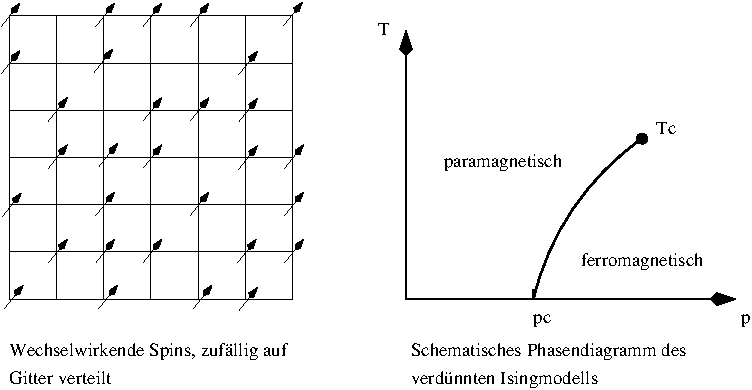
\includegraphics{./Einleitung-figs/diluted}
  \caption{Verd\"unntes Isingmodell}
  \label{fig:diluted}
\end{figure}

\section{Clusterzahlen}
Bei einem Perkolationsprozess auf einem Gitter entstehen in zuf\"alliger Weise zusammenh\"ang\-ende Bereiche. Zwei besetzte Vertices des Gitters sind verbunden, wenn sie n\"achste Nachbarn sind und die Gitterkante zwischen ihnen ge\"offnet ist. Eine maximale Menge von Vertices, die untereinander durch eine Kette von Vertices verbunden sind, hei"st Cluster. Wenn die Verteilung der Cluster bekannt ist, k\"onnen alle f\"ur die Perkolationstheorie relevanten Gr\"o"sen ausgerechnet werden.
\subsection{site-Perkolation in einer Dimension}
Auf einer eindimensionalen Kette von Vertices sind die einzigen m\"oglichen Cluster zusammenh\"angende St\"ucke der Kette. Jeder Cluster ist durch seine L\"ange vollst\"andig festgelegt. 
\begin{figure}[bp]
  \centering
  
\includegraphics{./Einleitung-figs/1d_simple}
  \caption{Kette von unbesetzten und besetzten Vertices. Es treten Cluster der Gr\"o"sen 1, 3 und 4 auf. Die Wahrscheinlichkeit dieser Anordnung ist $qpqqpppqppppq=p^8q^5$ ($q=1-p$). }
  \label{fig:1d_simple}
\end{figure}
Damit ein Vertex das linke Ende eines Clusters der Gr\"o"se $s$ ist, muss sein linker Nachbar unbesetzt, er selbst und seine $s-1$ rechten Nachbarn besetzt, und der darauffolgende Vertex wiederum unbesetzt sein (siehe Abb. \ref{fig:1d_simple}). Die Wahrscheinlichkeit dieses Ereignisses ist $n_s(p)=p^s(1-p)^2$. $n_s$ ist die erwartete Anzahl der Cluster der Gr\"o"se $s$ pro Vertex. Summiert man \"uber alle $s$, erh\"alt man die Gesamtzahl der Cluster pro Vertex
\begin{equation}
  n(p)=(1-p)^2\sum_{s=1}^\infty p^s=p(1-p).
\end{equation}
Ein besetzter Vertex ist unterhalb von $p_c$ in genau einem endlichen Cluster enthalten. Der Vertex kann an jedem der $s$ Pl\"atze eines Clusters der Gr\"o"se $s$ sein und die bedingte Wahrscheinlichkeit f\"ur dieses Ereignis ist $\mathcal{P}\{ x\in \text{Cluster der Gr\"o"se} \; s\:|\: x \; \text{ist besetzt}\}=sp^{s-1}(1-p)^2$. Jeder Vertex ist mit Wahrscheinlichkeit $p$ besetzt und es gilt\begin{equation}
  p=(1-p)^2\sum_{s=1}^\infty sp^s.
\end{equation}
Die mittlere Gr\"o"se des Clusters, zu dem ein beliebiger besetzter Vertex geh\"ort, ist durch
\begin{equation}
  S=\frac{(1-p)^2}{p}\sum_{s=1}^\infty s^2p^s=\frac{p+1}{p-1}
\end{equation}
gegeben. Die mittlere Clustergr\"o"se ist f\"ur $p<1$ endlich und divergiert im Limes vollst\"andiger Besetzung. Die Wahrscheinlichkeit, dass ein Vertex Teil eines Clusters der Gr\"o"se $s$ ist, ist f\"ur $p<1$ proportional zu $sp^s$. Im Limes unendlicher Clustergr\"o"se gilt
\begin{equation}
\lim_{s\rightarrow{\infty}} sn_s(p)= \begin{cases} 0 \qquad \text{f\"ur} \qquad p<1, \\ 1 \qquad \text{f\"ur} \qquad p=1. \end{cases}
\end{equation}
Daher ist in einer Dimension die triviale Perkolationsschwelle $p_c=1$, und es gibt keine perkolierende Phase. Die Euler-Charakteristik einer eindimensionalen Figur ist gleich der Zahl der Komponenten. Die mittlere Euler-Charakteristik pro Vertex is also $\chi(p)=n(p)=p(1-p)$. Ihre Nullstelle $p_0=1$ f\"allt mit $p_c$ zusammen.\\
Auch auf einem zweidimensionalen Gitterstreifen mit unendlicher Ausdehnung in horizontaler Richtung und endlicher H\"ohe $l$ tritt f\"ur $p<1$ kein unendlicher Cluster auf (siehe Abb. \ref{fig:1D}). Die Wahrscheinlichkeit, dass zwischen oberen und unteren Rand eine senkrechte Kette unbesetzter Gitterpl\"atzen exisitiert, ist $Q=(1-p)^l>0$. Damit ein Cluster eine horizontale L\"ange $s$ hat, d\"urfen an $s$ Stellen keine solchen Ketten auftreten. Daher ist die Wahrscheinlichkeit, dass ein Cluster mit horizontaler Ausdehnung $s$ auftritt, kleiner als $(1-Q)^s$ und verschwindet f\"ur gro"se $s$. \\
\begin{figure}[htbp]
  \centering
  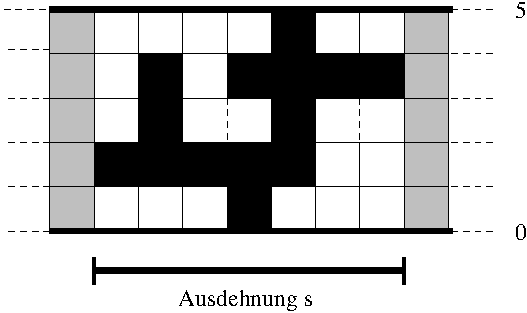
\includegraphics{./Einleitung-figs/1D}
  \caption{Cluster mit Ausdehnung $s$ auf einem Gitterstreifen der H\"ohe $l=5$; die Verbindungen von oben nach unten aus unbesetzten Gitterpl\"atzen sind in grau dargestellt. }
  \label{fig:1D}
\end{figure}
\subsection{Clusterzahlen in zwei Dimensionen}
\label{sec:animals}
W\"ahrend in einer Dimension ein Cluster nur durch seine L\"ange eindeutig beschrieben werden konnte, k\"onnen in zwei Dimensionen aus $s$ Vertices i. A. viele verschiedene Cluster gebildet werden. Damit ein bestimmter Cluster auftritt, m\"ussen alle Vertices, die zu ihm geh\"oren, besetzt und die umgebenden Vertices unbesetzt sein. Die Wahrscheinlichkeit, dass ein bestimmter Cluster auftritt, h\"angt also von seiner Masse $s$ und der L\"ange seines ``Perimeters'' $t$ ab und ist durch $p^s(1-p)^t$ gegeben. Cluster des Quadratgitters bis zur Masse $s=3$ sind in Abb. \ref{fig:2d_cluster} gezeigt. 
\begin{figure}[tbp]
  \centering
  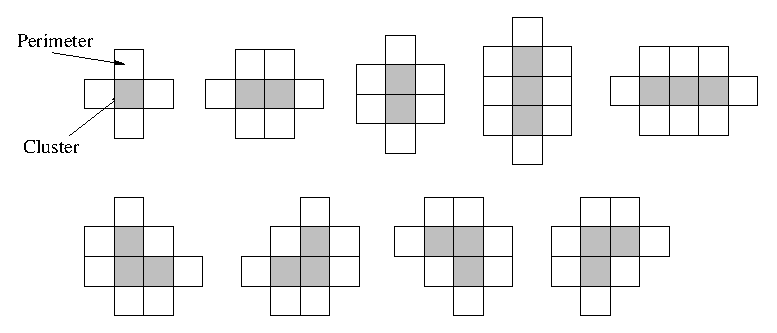
\includegraphics{./Einleitung-figs/2D_cluster}
  \caption{Cluster des Quadratgitters bis zur Masse $s=3$.}
  \label{fig:2d_cluster}
\end{figure}
Die erwartete Zahl der Cluster der Gr\"o"se $s$ pro Vertex ist mit $q=1-p$ f\"ur $s=1,2,3$
\begin{eqnarray}
n_1(p) & = & pq^4, \\
n_2(p) & = & 2p^2q^6, \\
n_3(p) & = & 2p^3q^8+4p^3q^7,
\end{eqnarray}
und allgemein
\begin{equation}
n_s(p)=\sum_t g_{st}p^sq^t=p^sD_s(p).
\end{equation}
Hierbei sind $g_{st}$ die Zahlen der Cluster der Masse $s$ und Umfangsl\"ange $t$. $D_s(p)=\sum_t g_{st}q^t$ sind die sogenannten Perimeterpolynome. Die Zahlen $g_{st}$ sind f\"ur verschiedene Gitter bis $s$ in der Gr\"o"senordnung von 20 mit Computern abgez\"ahlt worden. Bond-Perkolation kann auf dem \"Uberdeckungsgitter ganz analog als site-Perkolation behandelt werden.\\
Man kann die Cluster erzeugen, indem man, ausgehend von einem einzigen besetzten Vertex, sukzessive am Perimeter weitere Vertices besetzt. Dieser Prozess \"ahnelt der Vermehrung eines Zellhaufens durch Zellteilung. Daher werden diese Cluster oft \textbf{lattice animals} oder \textbf{Gittertiere} genannt.\\
Ein bestimmter besetzter Vertex kann jeder der $s$ Vertices eines Clusters der Masse $s$ sein und ist daher mit Wahrscheinlichkeit $sn_s(p)$ Teil eines solchen Clusters. Unterhalb von $p_c$ geh\"ort jeder besetzte Vertex zu einem endlichen Cluster, und da jeder Vertex mit Wahrscheinlichkeit $p$ besetzt ist, gilt
\begin{equation}
p=\sum_{s}sn_s(p) \qquad \text{f\"ur}\qquad p<p_c.
\end{equation}
In der perkolierenden Phase ist ein besetzter Vertex mit Wahrscheinlichkeit $P_\infty(p)$ Teil des unendlichen Cluster, und daher gilt
\begin{equation}
p=\sum_{s}sn_s(p)+P_\infty(p).
\end{equation}
Die mittlere Gr\"o"se der endlichen Cluster erh\"alt man in Analogie zum eindimensionalen Fall durch
 \begin{equation}
S_{endl}(p)=\frac{1}{p}\sum_{s}s^2n_s(p).
\end{equation}
Clusterzahlen in h\"oheren Dimensionen werden ganz analog zu denen in zwei Dimensionen definiert.

\subsection{Perkolation auf dem Bethe-Gitter}
Auf dem Bethe-Gitter l\"asst sich das Perkolationsproblem geschlossen l\"osen. Das Bethe-Gitter hat keine geschlossenen Schleifen, und zwischen zwei Vertices existiert \textbf{genau} eine Kette von Vertices, die beide Vertices verbindet. Die eindimensionale Kette ist ein spezielles Bethe-Gitters.
\begin{figure}[tbp]
  \centering
  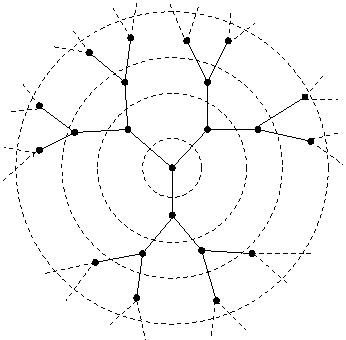
\includegraphics{./Einleitung-figs/bethe}
  \caption{Ein kleiner Auschnitt eines Bethe-Gitters mit $z=3$. Das Gitter l\"asst sich in Schalen $n=1,2,3,\ldots$ um den Ursprung zerlegen. }
  \label{fig:caley}
\end{figure}
\\Von einem Vertex des Bethe-Gitters gehen $z$ Verbindungen zu $z$ anderen Vertices, von diesen $z-1$ weitere Verbindungen zu neuen Vertices usw. (siehe Abb. \ref{fig:caley}). Von jedem Vertex gehen also $z$ \"Aste aus und der einzige gemeinsame Vertex dieser \"Aste ist der Ursprungsvertex. Dieser Vertex hat $z$ n\"achste Nachbarn, $z(z-1)$ \"ubern\"achste Nachbarn und $z(z-1)^{n-1}$ Vertices, die $n$ Schritte entfernt sind. Wir betrachten wiederum site-Perkolation und besetzen Vertices mit Wahrscheinlichkeit $p$.  Da zwei Vertices durch \textbf{genau} eine Kette von Vertices miteinander verbunden sind, ist die Wahrscheinlichkeit, dass zwei $n$ Schritte entfernte Vertices besetzt und verbunden sind durch $p^{n+1}$ gegeben. Es gibt gerade $z(z-1)^{n-1}$ $n$ Schritte entfernte Vertices und ein willk\"urlich ausgezeichneter Ursprung ist im Mittel mit $N_n=\frac{pz}{z-1}[p(z-1)]^n$ Vertices im Abstand $n$ verbunden. Gilt $p>\frac{1}{z-1}$, ist die Wahrscheinlichkeit, dass der Ursprung mit beliebig weit entfernten Vertices verbunden ist, gr\"o"ser $0$; ist $p<\frac{1}{z-1}$ verschwindet $N_n$ exponentiell mit $n$. Die Perkolationsschwelle liegt also bei $p_c=\frac{1}{z-1}$. Die mittlere Clustergr\"o"se erh\"alt man f\"ur $p(z-1)<1$ durch Summation der $N_n$ \"uber $n$
\begin{equation}
  \begin{split}
  S & = p+\frac{pz}{z-1}\sum_{n=1}^{\infty}[p(z-1)]^{n}=p+\frac{pz}{z-1}\left[\frac{1}{1-p(z-1)}-1\right] \\
  & =\frac{p(p+1)}{1-p(z-1)}=\frac{p_cp(1+p)}{p_c-p}.
\end{split}
\end{equation}
Die mittlere Clustergr\"o"se divergiert f\"ur $p\rightarrow p_c$ wie $S\sim \frac{1}{p_c-p}$. Der kritische Exponent $\gamma$ hat also den Wert 1. Auch die \"ubrigen Exponenten k\"onnen analog bestimmt werden, und man erh\"alt $\beta=1$ und $\nu=1/2$.\\ 
Die Zahl der Vertices, die weniger als $N+1$ Schritte vom Ursprung entfernt sind, ist f\"ur $z>2$ gleich $V=1+z\sum_{n=0}^{N-1}(z-1)^n=(z-1)^N$. Die Zahl der Vertices, die genau $N$ Schritte vom Ursprung entfernt sind, ist $A=z(z-1)^{N-1}$. $V$ und $A$ entsprechen dem Volumen und der Oberfl\"ache einer Kugel mit Radius $N$. In \"ublichen $d$-dimensionalen Gittern verh\"alt sich Kugeloberfl\"ache zu Kugelvolumen wie $A \sim V^{1-1/d}$. F\"ur gro"se $d$ sind Oberf\"ache und Volumen also fast proportional zueinander. Daher kann das Bethe-Gitter mit $z>2$ als Modell f\"ur Gitter hoher Dimension aufgefasst werden. Tats\"achlich stimmen die kritischen Exponenten der Perkolation auf dem Bethe-Gitter mit denen auf Gittern mit $d>19$ \"uberein. Vermutlich gilt diese \"Ubereinstimmung sogar herab bis $d=6$. F\"ur $z=2$ wird der eindimensionale Fall reproduziert. \\
Bond-Perkolation wird ganz analog behandelt und man erh\"alt die gleiche Perkolationsschwelle.\\  
Die Euler-Charakteristik eines Baumgraphen ist (zur Euler-Charakteristik siehe Kapitel \ref{sec:Euler}) die Differenz der Zahl der Vertices und Kanten. Betrachtet man die Vertices und Kanten innerhalb von $N$ Schalen um den Ursprung, kann die mittlere Euler-Charakteristik des Graphens in diesem Beobachtungsfenster bestimmt werden. Bei der site-Perkolation werden Vertices mit Wahrscheinlichkeit $p$ besetzt und eine Kante zwischen zwei Vertices ist mit Wahrscheinlichkeit $p^2$ vorhanden. Entsprechend sind bei bond-Perkolation alle Vertices besetzt, und Kanten sind mit Wahrscheinlichkeit $p$ vorhanden. Beide F\"alle unterscheiden sich also nur durch einen Faktor $p$. F\"ur die Euler-Charakteristik bei site-Perkolation ergibt sich
\begin{equation}
  \chi^{site}_N(p)=p\left[1+z\sum_{n=1}^N(z-1)^{n-1}\right]-p^2\left[z\sum_{n=1}^{N+1}(z-1)^{n-1}\right].
\end{equation}
Hierbei wurden alle Kanten, die aus dem Beobachtungsfenster hinausf\"uhren, mitgez\"ahlt. Die Nullstelle $p_0$ konvergiert f\"ur $N\rightarrow \infty$ gegen $\frac{1}{z-1}$. Das gleiche Resultat gilt im Fall der bond-Perkolation. Wie bei Perkolation in einer Dimension, stimmt $p_0$ mit $p_c$ auf dem Bethe-Gitter \"uberein.\\ 

\section{Perkolationsschwellen}

Nachdem Perkolation in groben Z\"ugen vorgestellt wurde, wird im Folgenden Bekanntes zu Perkolationsschwellen zusammengetragen. 

\subsection{Rigorose Ungleichungen}
Im Allgemeinen sind f\"ur Perkolationsschwellen nur sehr grobe Ungleichungen bekannt. Nichttriviale, allgemein g\"ultige Ungleichungen sind $p_c^{site}\geq p_c^{bond}$ und $p_c^{bond}\geq \frac{1}{\mu} \geq \frac{1}{z-1}$, wobei $\mu$ die Konnektivit\"atszahl und $z$ die Koordinationszahl des betrachteten Gitters ist. Die Konnektivit\"atszahl ist durch $\mu=\lim_{n\rightarrow \infty}\frac{\ln N_{SAW}^n}{n}$ definiert, wobei $N_{SAW}^n$ die Zahl der selbstvermeidenden Wege der L\"ange $n$ auf dem betrachteten Gitter ist. In zwei Dimensionen folgt aus der matching-Eigenschaft (siehe unten) eine obere Schranke an $p_c^{site}$. Da Gitter der Dimension $d$ perkolieren, wenn $(d-1)$-dimensionale Untergitter perkolieren, k\"onnen Perkolationschwellen mit $d$ h\"ochstens abnehmen, sind aber echt gr\"o"ser als $0$. F\"ur alle Gitter mit $d \geq 2$ gilt also $0 < p_c^{bond} \leq p_c^{site}<1$. Auf allen Gittern in $d\geq 2$ existiert daher eine nicht perkolierende Phase $p<p_c$ und einen Bereich $p>p_c$, in dem ein unendlicher Cluster exisitert. Auf einige Gitter, deren Perkolationsschwellen exakt bekannt sind, wird im Kapitel \ref{sec:dualitaet} genauer eingegegangen. F\"ur site-Perkolation auf dem Quadrat-, dice- und Sechseckgitter, sowie f\"ur bond-Perkolation auf dem Kagom\'egitter existieren rigorose obere und untere Schranken f\"ur die Perkolationschwellen. Diese Schranken und die zugeh\"origen Referenzen sind Referenz \cite{Hughes:96} entnommen. 
\begin{eqnarray}
& 0.5416\leq p_c^{sq-site}\leq0.6795 & \quad \text{Wierman \cite{Wierman:95}, Men'shikov und Pelikh \cite{Menshikov:89}}\\
& p_c^{hex-bond}\leq p_c^{hex-site}\leq 0.8079  &\quad \text{Luczak und Wiermann \cite{Luczak:88}}\\
& 0.5182 \leq p_c^{kag-bond}\leq 0.5335 & \quad \text{Wierman \cite{Wierman:90}}\\
& 0.520 \leq p_c^{dice-site}\leq 0.7937 &\quad \text{Luczak und Wiermann \cite{Luczak:88}}
\end{eqnarray}
Um diese Schranken herzuleiten, ist erheblicher mathematischer Aufwand n\"otig. Dar\"uberhinaus sind wenig rigorose Resultate \"uber Perkolationsschwellen bekannt.  


\subsection{Dualit\"at und matching -- exakte Perkolationsschwellen}
\label{sec:dualitaet}
In zwei Dimensionen sind einige Perkolationsschwellen exakt bekannt. Die exakte Bestimmung der Perkolationsschwellen beruht auf der Tatsache, dass es zu jedem zweidimensionalen Gitter ein sog. \textit{duales Gitter} gibt, und die Perkolationsschwellen dieser beiden Gittern miteinander in Verbindung gebracht werden k\"onnen. 
\\Ein planarer Graph $G$ l\"asst sich in die Ebene einbetten, ohne dass sich zwei Kanten schneiden (f\"ur eine Definition dieser Begriffe siehe \ref{sec:graphen} oder \cite{Essam:70}). Der Graph zerschneidet die Ebene in endliche Gebiete. Setzt man in jedes dieser endlichen Gebiete und in das Gebiet au"serhalb des Graphens einen Vertex und verbindet Vertices, deren Gebiete sich an einer Kante von $G$ ber\"uhren, erh\"alt man den dualen Graphen $G^*$ (siehe Abb. \ref{fig:dualgraph}).
\begin{figure}[htbp]
  \centering
  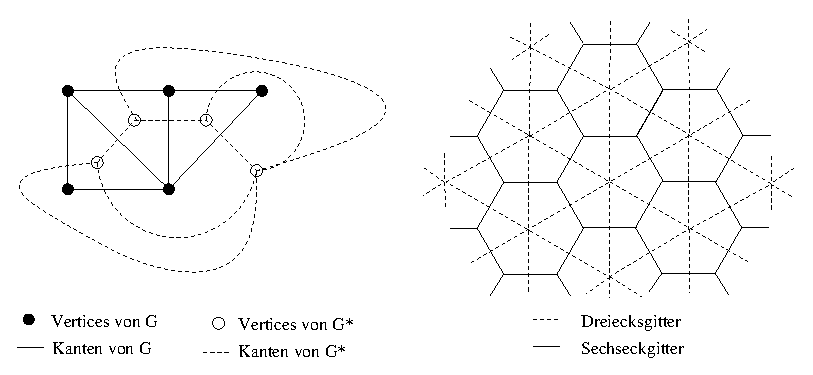
\includegraphics{./Einleitung-figs/dualgraph}
  \caption{Links: Jede Kante des Graphen $G$ wird von einer Kante des dualen Graph $G^*$ geschnitten. Rechts: Das Dreiecks- und Sechseckgitter bilden ein Paar dualer Gitter.}
  \label{fig:dualgraph}
\end{figure}
Die Dualit\"atstransformation stiftet eine eins-zu-eins-\-Korrespondenz zwischen den Kanten des Graphen und denen des dualen Graphens. Zweidimensionale Gitter sind periodisch fortgesetzte Graphen und zu jedem Gitter $\mathcal{G}$ kann ein duales Gitter $\mathcal{G}^*$ konstruiert werden. Wir interessieren uns f\"ur Paare dualer Gitter. Jede Kante in $\mathcal{G}^*$ schneidet genau eine Kante in $\mathcal{G}$ und die Kantenmengen $E$ und $E^*$ von $\mathcal{G}$ und $\mathcal{G}^*$ k\"onnen identifiziert werden. Ihre Vertexmengen $V$ und $V^*$ sind aber i. A. unterschiedlich.\\
Wir betrachten nun bond-Perkolation auf $\mathcal{G}$ und besetzen einen Teil der Kanten $E'\subset E$ von $\mathcal{G}$. Es entsteht eine Subgraph $G$ mit Vertexmenge $V$ und Kantenmenge $E'$. Da jede Kante aus $\mathcal{G}$ eine Kante aus $\mathcal{G}^*$ schneidet, betrachten wir nun den Subgraph $G^*$ von $\mathcal{G}^*$ mit Vertexmenge $V^*$ und Kantenmenge $E^{*'}=E\backslash E'$. Die Komponenten von $G$ bzw. $G^*$ sind Cluster auf den Gittern $\mathcal{G}$ bzw. $\mathcal{G}^*$. Jeder endliche Cluster auf $\mathcal{G}$ ist von einem Cluster auf $\mathcal{G}^*$ umschlossen, denn alle unbesetzten Kanten am Rand eines Clusters werden von besetzten dualen Kanten geschnitten. Umgekehrt gilt dasselbe (siehe Abb. \ref{fig:dual}). Betrachtet man einen gro"sen rechteckigen Ausschnitt des Gitters, so existiert ein Cluster auf $\mathcal{G}$, der den linken und rechten Rand des Rechtecks verbindet, genau dann, wenn kein solcher Cluster auf $\mathcal{G}^*$ den oberen und unteren Rand verbindet. Besetzt man Kanten von $\mathcal{G}$ mit Wahrscheinlichkeit $p$, so entsteht ein komplement\"ares Perkolationsproblem mit Besetztungswahrscheinlichkeit $q=1-p$ auf $\mathcal{G}^*$. F\"ur die Perkolationschwellen gilt 
\begin{equation}
  p_c^{bond}(\mathcal{G})+p_c^{bond}(\mathcal{G}^*)=1.
\end{equation}
Das Quadratgitter ist ``selbstdual'' und $p_c=\frac{1}{2}$ (siehe Abb. \ref{fig:dual}). Das Dreiecks- und das Sechseckgitter sind ein duales Paar und k\"onnen durch die sogenannte Stern-Dreiecks-Transformation ineinander \"uberf\"uhrt werden. Dadurch erh\"alt man f\"ur $p_c$ eine zus\"atzliche Gleichung und die L\"osung $p_c^{Dreieck}=1-p_c^{Sechseck}=2\sin(\pi/18)$. Diese \"Uberlegungen gehen auf Sykes und Essam \cite{Sykes:64} zur\"uck, sind aber nicht im mathematischen Sinne rigoros. Wierman \cite{Wierman:84} hat eine verallgemeinerte Stern-Dreieckstransformation auf das bowtie-Gitter angewendet. Die bond-Perkolationsschwelle $p_c$ ist die L\"osung von $1-p-6p+6p^3-p^5=0$ und hat den numerischen Wert $p_c=0.404518\ldots$.
\begin{figure}[htbp]
  \centering
  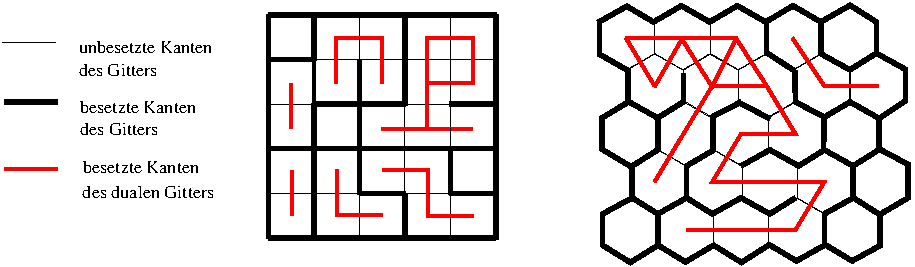
\includegraphics{./Einleitung-figs/dualnew}
  \caption{Komplement\"are Besetzung der Kanten eines Paares dualer Gitter am Beispiel des selbstdualen Quadratgitters und des Dreiecks- und Sechseckgitters.}
  \label{fig:dual}
\end{figure}
\\Jedem bond-Perkolationsproblem entspricht ein site-Perkolationsproblem auf dem \"Uberdeckungsgitter (siehe Abb. \ref{fig:covering_einleit}). Also sollte sich die Dualit\"ats-Eigenschaft auf die site-Perkolation \"ubertragen lassen. Dies ist in der Tat m\"oglich, allerdings muss der Gitterbegriff auf nichtplanare Gitter, sog. ``dekorierte Mosaike'', verallgemeinert werden. Man geht von einem planaren Gitter, im folgenden \textit{Mosaik} genannt, aus und erg\"anzt bei einem Teil der Plaketten alle diagonalen Verbindungen. Eine solche Plakette hei"st \textit{dekoriert} und das resultierende, im Allgemeinen nicht mehr planare, Gitter \textit{dekoriertes Mosaik}. Das matching-Gitter  $\mathcal{G}^+$ zu einem dekorierten Mosaik $\mathcal{G}$ erh\"alt man, indem das Mosaik komplement\"ar dekoriert wird, d.h. die Plaketten die in $\mathcal{G}$ nicht dekoriert waren, werden in $\mathcal{G}^+$ dekoriert und umgekehrt (siehe Abb. \ref{fig:matchinggitter}). 
\begin{figure}[tbp]
  \centering
  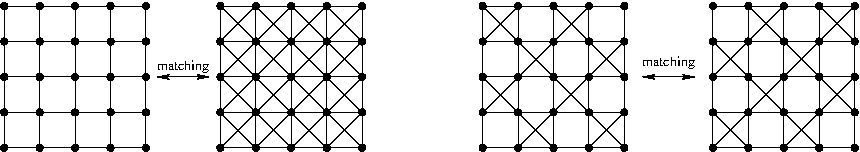
\includegraphics{./Einleitung-figs/matchinggitter}
  \caption{Links: Ein Vertex des Quadratgitters hat vier n\"achste Nachbarn, einer des matching-Gitters acht. Rechts: Die Gitter sind selfmatching. Sie sind das \"Uberdeckungsgitter des Quadratgitters.}
  \label{fig:matchinggitter}
\end{figure}
$\mathcal{G}=(V,E)$ und $\mathcal{G}^+=(V,E^+)$ haben die gleiche Vertexmenge, aber i. A. unterschiedliche Kantenmengen. Die Kanten des Mosaiks sind in $E$ und $E^+$ enthalten. Die Graphen $G$ und $G^+$ mit Vertexmengen $I \subset V$ und $I^+=V \backslash I$ und Kantenmengen $K=\{x,y\in I|xy \in E\}$ und $K^+=\{x,y\in I^+|xy \in E^+\}$ haben die entsprechende Dualit\"atseigenschaft: Jede endliche Komponente von $G$ ist in einem geschlossenen Weg in $G^+$ enthalten; dies gilt in analoger Weise umgekehrt (siehe Abb. \ref{fig:matching}). Die site-Perkolationsschwellen zweier matching-Gitter erg\"anzen sich zu 1. Aus der matching-Eigenschaft kann man einfach eine nichtriviale obere Schranke an die site-Perkolationsschwelle gewinnen, denn $p_c^{site}(\mathcal{G})=1-p_c^{site}(\mathcal{G}^+) \leq 1-\frac{1}{\mu^+}\leq 1-\frac{1}{z^+-1}<1$.\\
Das Dreiecksgitter ist selfmatching, denn alle Ecken eines Dreiecks sind Nachbarn, und es gibt keine Verbindungen, die erg\"anzt werden k\"onnten. Daher ist die site-Perkolationsschwelle des Dreiecksgitters $p_c=\frac{1}{2}$. Im matching-Gitter eines planaren Gitters sind alle Plaketten dekoriert und daher alle Vertices auf dem Rand einer Plakette n\"achste Nachbarn (siehe linker Teil in Abb. \ref{fig:matchinggitter}). Ein planares Gitter ist immer ein Subgraph seines matching-Gitters und hat daher eine h\"ohere Perkolationsschwelle als sein matching-Gitter. Daher ist $p_c^{site} \geq \frac{1}{2}$ f\"ur alle planaren Gitter.
Das Kagom\'e-Gitter ist das \"Uberdeckungsgitter des Sechseckgitters, und es gilt $p_c^{site-Kagome}=p_c^{bond-Sechseck}$. \\
\begin{figure}[htbp]
  \centering
  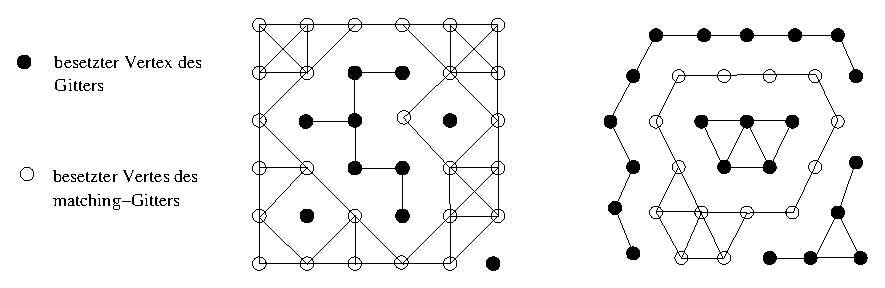
\includegraphics{./Einleitung-figs/match}
  \caption{Komplement\"ar besetzte Paare von matching-Gittern am Beispiel des Quadrat- und Dreiecksgitters.}
  \label{fig:matching} 
\end{figure}


\subsection{Empirische Formeln f\"ur Perkolationsschwellen}
In Literatur \"uber Perkolation sind des \"ofteren empirische Formeln f\"ur Perkolationsschwellen in Abh\"angigkeit von Koordinationszahl $z$ und Dimension $d$ vorgestellt worden. F\"ur bond-Perkolation gilt in zwei Dimensionen als grobe N\"aherung $p_c\approx \frac{2}{z}$, f\"ur hoch-dimensionale Gitter $p_c \approx \frac{1}{z-1}$. Andere Formeln enthalten eine Reihe von Fitparametern und sagen $p_c$ als Funktion von $d$ und $z$ voraus. Tats\"achlich variieren Perkolationsschwellen auf Gittern der gleichen Dimension und gleicher Koordinationszahl betr\"achtlich, so dass eine Vorhersage von Perkolationsschwellen allein aus $d$ und $z$ nicht sinnvoll erscheint. \\
Scher und Zallen \cite{Scher:70} beobachteten einen Zusammenhang zwischen site-Perkolationsschwel\-len und der Packungsdichte $f$ f\"ur zwei- und dreidimensionale Gitter. Die Packungsdichte ist der Anteil des Raums (Ebene), der bedeckt ist, wenn auf jeden Vertex des Gitters eine Kugel (Kreisscheibe) mit Radius der halben Kantenl\"ange sitzt. F\"ur das \mbox{Quadrat-,} \mbox{Dreiecks-,} Sechseck- und Kagom\'egitter fanden Scher und Zallen $fp_c \sim 0.44$; in drei Dimensionen f\"ur das sc-, bcc- und fcc-Gitter $fp_c \sim 0.15$. Suding und Ziff \cite{Suding:99} haben diesen Zusammenhang auf alle archimedischen Gitter (siehe Abschnitt \ref{sec:archilattices}) ausgedehnt. Dazu konstruieren sie aus Gittereigenschaften ein generalisiertes $f$ und schlagen ein quadratisches Polynom in $f$ als empirische Formel f\"ur $p_c$ vor. F\"ur beide Formeln ist ein Fit an bekannte Perkolationsschwellen n\"otig. Daher h\"angen die Vorhersagen der Formeln von den f\"ur den Fit verwendeten Perkolationsschwellen ab. Eine Methode, Perkolationsschwellen ohne die Notwendigkeit eines Fits an bekannte Schwellen vorhersagen zu k\"onnen, ist daher w\"unschenswert. Eine solche Mehtode ist von Balberg \textit{et al.} \cite{Balberg:91} f\"ur Kontinuumsperkolation vorgeschlagen worden. Aus der Bedingung, dass die mittlere Zahl der Nachbarn der Konstituenten einen bestimmten Wert \"ubersteigt, wird ein Perkolationskriterium abgeleitet. Eine andere M\"oglichkeit Vorhersagen von Perkolationsschwellen zu machen, bietet die mittlere Euler-Charakteristik  der Perkolationskonfigurationen.   

\section{Euler-Charakteristik und Perkolation}

Wie eingangs erw\"ahnt, war zu Beginn dieser Arbeit f\"ur eine Reihe von site-Perkolations"-pro"-blemen empirisch bekannt, dass die Nullstelle der mittleren Euler-Charakteristik in der N\"ahe der Perkolationsschwelle liegt \cite{Wagner:02}. F\"ur Kontinuumsperkolation wurde \"uber die Beziehung zwischen Euler-Charakteristik und Perkolation erstmals in Ref. \cite{Mecke:91} berichtet. Die prominentesten Beispiele dieses Befundes sollen hier als Ausgangsbasis vorgestellt werden. Die Mittelwerte der Euler-Charakteristik sind f"ur Konfigurationen, die in einem Perkolationsproblem mit Besetzungswahrscheinlichkeit $p$ entstehen, Polynome in $p$. Wie man diese Polynome berechnet, wird im Abschnitt \ref{sec:chimittel} dargelegt. 

\subsection{Zwei Dimensionen - archimedische Gitter}
\label{sec:archilattices}
Es gibt genau elf zweidimensionale Gitter \cite{Gruenbaum:86}, die nur aus regelm"a"sigen Polygonen der gleichen Kantenl\"ange bestehen, und deren Vertices alle "aquivalent sind. Diese Gitter hei"sen archimedische Gitter und sind in Abbildung \ref{fig:archimed} dargestellt.
\begin{figure}[tbp]
  \centering
  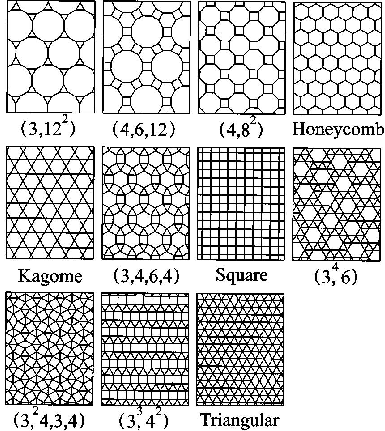
\includegraphics{./Einleitung-figs/archimed}
  \caption{Die elf archimedischen Gitter. Die Zahlenfolgen unter den Gitterausschnitten sind die Vertexkonfigurationen der Gitter, die keine gebr\"auchlichen Namen haben (siehe Text). Die Abbildung wurde aus \cite{Suding:99} \"ubernommen.}
  \label{fig:archimed}
\end{figure}
Da die Umgebungen aller Vertices bis auf eine Drehung identisch sind, lassen sich die Gitter durch die Folge $(n_1,\ldots,n_z)$ der Eckenzahlen der Polygone, die einen Vertex im Uhrzeigersinn umgeben, charakterisieren. Folgen $a_i$ gleiche Polygone aufeinander, so wird kurz $n_i^{a_i}$ geschrieben. Im Dreiecksgitter umgeben jeden Vertex sechs Dreiecke und die Vertexkonfiguration ist $(3^6)$. Analog sind die Vertexkonfigurationen des \mbox{Quadrat-,} des \mbox{Sechseck-} und des Kagom\'egitters,  $(4^4)$, $(6^3)$ bzw. $(3,6,3,6)$. F\"ur die \"ubrigen Gitter siehe Abb. \ref{fig:archimed}.
\\Die Euler-Charakteristik einer zweidimensionalen Figur ist die Differenz der Zahl der Komponenten der Figur und der Zahl der L"ocher in diesen Komponenten. Die mittlere Euler-Charakteristik $\chi(p)$ von Perkolationskonfigurationen auf Gittern ist also die mittlere Zahl der Cluster, abz\"uglich der mittleren Zahl der L\"ocher in diesen Clustern. Die mittlere Euler-Charakteristik des Quadratgitters ist links in Abbildung \ref{fig:chieinleit} dargestellt. Die mittleren Euler-Charakteristiken aller archimedischen Gitter sind bekannt \cite{Wagner:02}, und haben eine Nullstelle $p_0$ zwischen 0 und 1. Auch die site-Perkolationsschwellen $p_c$ aller archimedischen Gitter \cite{Suding:99} sind bekannt. Die Nullstelle $p_0$ liegt bei allen archimedischen Gittern knapp \"uber $p_c$. Dar\"uberhinaus liegt der Wendepunkt $p_0^{(2)}$ der Euler-Charakteristik knapp unter $p_c$, und das arithmetische Mittel aus Nullstelle und Wendepunkt liefert eine exzellente Approximation von $p_c$. Diese Befunde sind in  Tabelle \ref{tab:archisite} und Abbildung \ref{fig:archisite} zusammengetragen.\\
\begin{table}[htbp]
\centering
  \begin{tabular}{|l|r|r|r||r|}
    \hline
    Vertexkonfiguration &$p_0$ &$p_0^{(2)}$ &$\frac{p_0+p_0^{(2)}}{2}$& $p_c$ \cite{Suding:99} \\ \hline
    \hline

    $3,12^2$ &$0.8395$ &$0.7631$&$0.80131$&$0.8079$ \\ \hline

    $4,6,12$&$0.7833$ &$0.7012$ &$0.74227$&$0.7478$\\ \hline

    $4,8^2$&$0.7689$ &$0.6935$ &$0.73120$&$0.7292$\\ \hline

    $6^3$ Sechseckg. &$0.7413$&$0.6687$ &$0.70501$&$0.6970$\\ \hline

    $3,6,3,6$ Kagom\'eg.&$0.6756$&$0.6231$ &$0.64936$&$0.6527$ \\ \hline

    $3,4,6,4$ &$0.6468$&$0.5994$ &$0.62311$&$0.6218$ \\ \hline

    $4^4$ Quadratg.&$0.6180$&$0.5774$ &$0.59769$&$0.5927$\\ \hline

    $3^4,6$  &$0.5913$&$0.5625$  &$0.57686$& $0.5750$\\ \hline

    $3^2,4,3,4$ &$0.5616$ &$0.5408$ &$0.55119$&$0.5508$ \\ \hline

    $3^3,4^2$ &$0.5616$&$0.5408$ &$0.55119$&$0.5502$  \\ \hline

    $3^6$ Dreiecksg. &$\frac{1}{2}$&$\frac{1}{2}$&$\frac{1}{2}$ &$\frac{1}{2}$\\ \hline

    \hline
  \end{tabular}
  \caption{Euler-Charakteristik und site-Perkolation auf archimedischen Gittern: Die Nullstellen $p_0$ und die Wendepunkte $p_0^{(2)}$ der mittleren Euler-Charakteristik archimedischer Gitter sind obere bzw. untere Schranken f\"ur die site-Perkolationsschwellen $p_c$. Das arithmetische Mittel aus $p_0$ und $p_0^{(2)}$ ist eine exzellente Approximation von $p_c$.}
  \label{tab:archisite}
\end{table}
\begin{figure}[htbp]
  \centering
  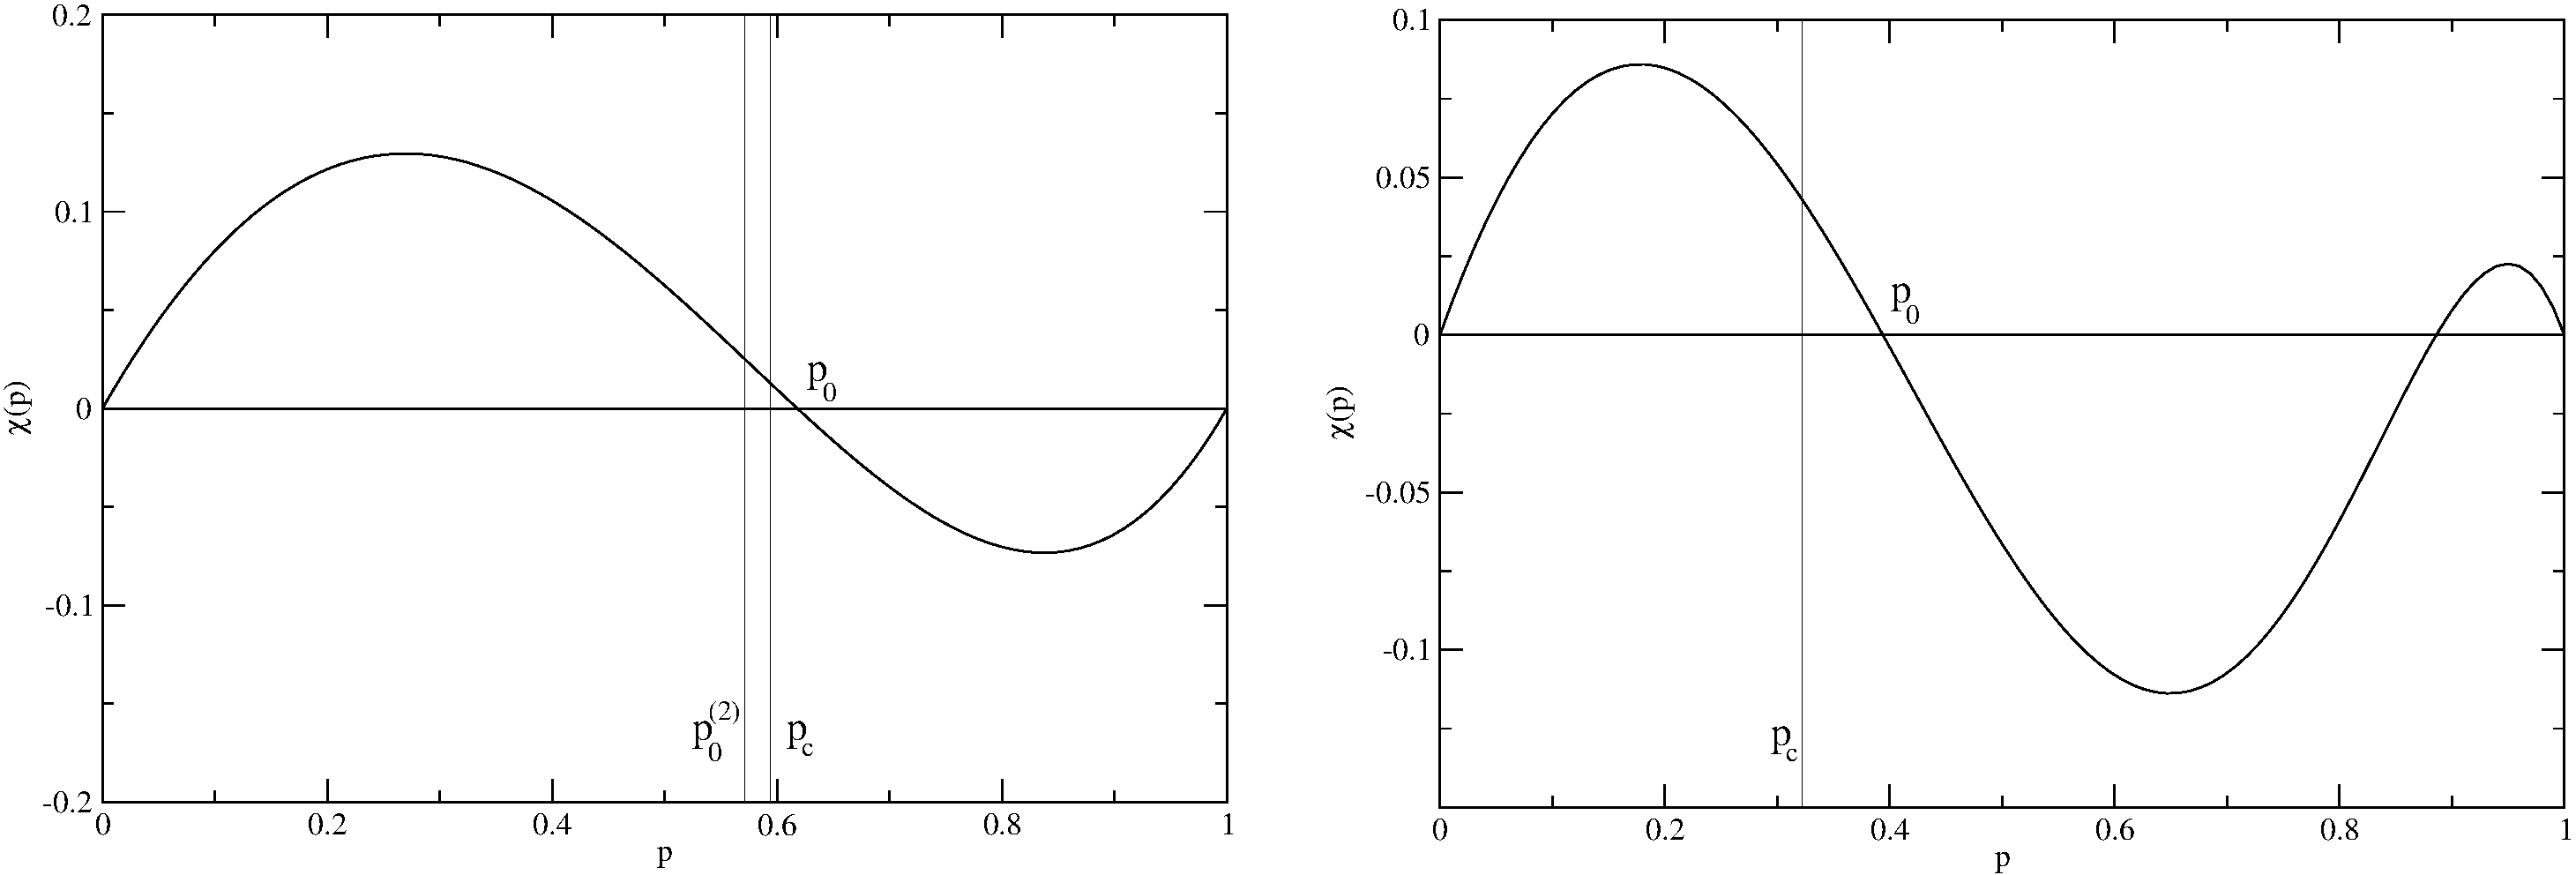
\includegraphics[width=5.5in]{./Einleitung-figs/chi}
  \caption{Die mittlere Euler-Charakteristik pro Vertex $\chi(p)$ des zweidimensionalen Quadratgitters (links) und des dreidimensionalen einfach kubischen Gitters (rechts). Die Nullstelle $p_0$ von $\chi(p)$, die Perkolationsschwellen $p_c$ der Gitter, sowie im zweidimensionalen Fall der Wendepunkt $p_0^{(2)}$ von $\chi(p)$ sind jeweils markiert.}
  \label{fig:chieinleit}
\end{figure}


\begin{figure}[htbp]
  \centering
  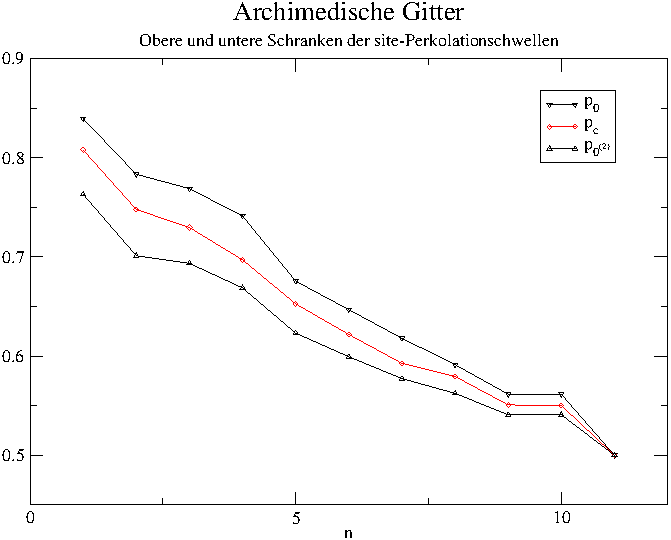
\includegraphics[width=5.5in]{./Einleitung-figs/archisitesingle}
  \caption{Die site-Perkolationsschwellen $p_c$ archimedischer Gitter liegen zwischen der Nullstelle $p_0$ und dem Wendepunkt $p_0^{(2)}$ der mittleren Euler-Charakteristik.}
  \label{fig:archisite}
\end{figure}


\subsection{Dreidimensionale Gitter}
Die Euler-Charakteristik einer dreidimensionalen Figur ist die Zahl der Komponenten, minus der Zahl der Henkel, plus der Zahl der Einschl"usse der Figur. F\"ur Perkolationskonfigurationen auf Gittern l\"asst sich eine mittlere Euler-Charakteristik $\chi(p)$ berechnen. In drei Dimensionen hat $\chi(p)$ zwei Nullstellen zwischen $0$ und $1$. Die mittlere Euler-Charakteristik ist f\"ur kleine $p$ (isolierte Cluster \"uberwiegen) und f\"ur $p$ nahe $1$ (Einschl\"usse \"uberwiegen) positiv. Zwischen diesen beiden Bereichen ist $\chi(p)$ negativ. Die mittlere Euler-Charakteristik des einfach kubischen Gitters ist rechts in Abbildung \ref{fig:chieinleit} dargestellt. Die kleinere Nullstelle der Euler-Charakteristik liegt beim einfach-kubischen (sc-) Gitter mit sechs und $26$ Nachbarn, beim fcc- mit $12$ und beim bcc-Gitter mit $14$ Nachbarn \"uber der Perkolationsschwelle (siehe Tabelle \ref{tab:3Dknown}). Der erste Wendepunkt von $\chi(p)$ liegt bei diesen Gittern \"uber der Perkolationsschwelle und liefert leider keine untere Schranke. 
\begin{table}[btp]
  \centering
  \begin{tabular}{|l|r|r||r|}
    \hline
    Gitter & \# Gitternachbarn &$p_0$ & $p_c$ \\ \hline
    sc & $6$  &$ 0.397 $& $0.3114(4)$ \\ \hline 
    sc & $26$ &$ 0.114 $& $0.097$  \\ \hline 
    bcc & $14$  &$ 0.211 $& $0.175$ \\ \hline 
    fcc & $12$  &$ 0.237 $& $0.1994(2)$ \\ \hline 

  \end{tabular}
  \caption{Dreidimensionale Gitter: Nullstellen $p_0$ der Euler-Charakteristik verglichen mit den Perkolationsschwellen $p_c$. Die Werte der Perkolationsschwellen des sc-Gitters mit 6 und des fcc-Gitter mit 12 Nachbarn stammen aus \cite{Marck:97}, die \"ubrigen aus \cite{Essam:72}. Letztere sind vermutlich sehr ungenau.}
  \label{tab:3Dknown}
\end{table}

\subsection{Hyperkubische Gitter}
Durch eine Rekursion l\"asst sich die mittlere Euler-Charakteristik hyperkubischer Gitter beliebiger Dimension $d$ ausrechnen (siehe Mecke \cite{Mecke:94} oder Jung \cite{Jung:00}). Aus
\begin{equation}
  \chi^d(p)=\sum_{i=0}^d (-1)^i{ d \choose i} p^{2^i}=p-dp^2+\frac{d(d-1)}{2}p^4-\cdots
\end{equation}
erh\"alt man f\"ur gro"se $d$ $p_0 \approx \frac{1}{d} =\frac{2}{z}$. Mit steigender Dimension des Gitters sollte sich die Perkolationsschwelle der des Bethe-Gitters $p_c=\frac{1}{z-1}$ ann\"ahern. Daher gilt f\"ur Perkolationsschwellen hoch-dimensionaler hyperkubischer Gitter $p_0\approx 2p_c$.


\subsection{Kontinuumsperkolation}
Mit Methoden der Integralgeometrie (\cite{Mecke:91} und \cite{Mecke:94}) kann die mittlere Euler-Charakteristik des Boolschen Kornmodells exakt bestimmt werden. Im Boolschen Kornmodell werden Punkte nach einem Poissonprozess mit Punktdichte $\rho$ verteilt und an diese Punkte unabh\"angig voneinander konvexe K\"orper angeheftet. Die mittlere Euler-Charakteristik h\"angt neben der Punktdichte $\rho$ auch von geometrischen Eigenschaften der K\"orper ab. In zwei Dimensionen geht das Verh\"altnis von Umfang $u$ und Fl\"ache $f$ der K\"orper in die Euler-Charakteristik ein, und mit $I=\frac{u^2}{4\pi f}$ erh\"alt man f\"ur die Euler-Charakteristik pro Fl\"ache
\begin{equation}
  \chi_2(\eta)=\eta(1 - I\eta)e^{-\eta}.
\end{equation}
Hier ist $\eta$ das Produkt aus $\rho$ und der Fl\"ache der K\"orper. In drei Dimensionen h\"angt $\chi$ vom Verh\"altnis der Oberfl\"ache $f$ und der mittleren integralen Kr\"ummung $h$ zum Volumen $v$ ab. Mit $I_1=\frac{fh}{12\pi v}$, $I_2=\frac{f^3}{36\pi v^2}$ und $\eta=\rho v$ ist die Euler-Charakteristik pro Volumen 
 \begin{equation}
  \chi_3(\eta)=\eta(1-3I_1\eta + \frac{3\pi^2}{32}I_2\eta^2)e^{-\eta}.
\end{equation}
 \\
Die Perkolationsschwellen $\eta_c$ des Boolschen Kornmodells monodisperser Kugeln ist in zwei und drei Dimensionen numerisch bekannt und die Nullstelle $\eta_0$ von $\chi_d(\eta)$ liegt zwei Dimensionen knapp unter und in drei Dimensionen knapp \"uber $\eta_c$.\\

\noindent
Auf Kontinuumsperkolation und hyperkubische Gitter wird im Folgenden nicht mehr eingegangen. Sie werden hier nur der Vollst\"andigkeit halber beschrieben. In dieser Arbeit werden die empirischen Beobachtungen, dass
\textbf{ %
\begin{itemize}
\item die Perkolationsschwellen zweidimensionaler Gitter zwischen der Nullstelle und dem Wendepunkt der mittleren Euler-Charakteristik liegen,
\item  die Nullstelle der mittleren Euler-Charakteristik dreidimensionaler Gitter \"uber deren Perkolationsschwelle liegt,
\end{itemize} %
}
\noindent untersucht. Im folgenden Kapitel wird zun\"achst die Euler-Charakteristik genauer betrachtet.

  %8.9.03

\chapter{Euler-Charakteristik}
\label{sec:Euler}

F"ur die Anzahl der Ecken $e$, die der Kanten $k$ und die der Fl"achen $f$ eines W"urfels gilt $e-k+f=2$. Teilt man eine Fl\"ache des W\"urfels, entstehen neue Ecken oder Kanten, die den Beitrag der zus\"atzlichen Fl\"ache wegheben, und es gilt weiterhin $e-k+f=2$. Der Eulerschen Polyedersatz besagt, dass diese Beziehung f"ur alle konvexen Polyeder $P$ gilt \cite{Saskin:89}. F\"ur eine Figur $F$, die nur aus Fl\"achen, Kanten und Ecken besteht, definiert man die Euler-Charakteristik durch
\begin{equation}
  \chi(F):=e-f+k.
\end{equation}
Die Euler-Charakteristik ist unabh\"angig von der Zerlegung und daher eine topologische Invariante von $F$. Deformiert  man $F$, bleibt $\chi(F)$ konstant. Es gibt eine Reihe von M\"oglichkeiten, die Euler-Charakteristik einer gegebenen Figur auszurechnen. Im ersten Teil des Kapitels werden die Facetten von $\chi$, die f\"ur diese Arbeit relevant sind, vorgestellt. Der zweite Teil besch\"aftigt sich mit Methoden, die Euler-Charakteristik von Gitterclustern auszurechnen.

\section{Euler-Charakteristik auf dem Konvexring}
Die Euler-Charakteristik wurde von Hadwinger \cite{Hadwinger:57} axiomatisch f\"ur alle endlichen Vereinigungen und Durchschnitte konvexer K\"orper eingef\"uhrt.
Ein $d$-dimensionaler konvexer K\"orper ist eine kompakte, d.h. beschr\"ankte und abgeschlossene, konvexe Teilmenge des $\mathbb{R}^d$, die in keiner nieder-dimensionalen affinen Hyperebene enthalten ist. Man definiert f\"ur alle konvexen K\"orper $A$ die Euler-Charakteristik durch $\chi(A):=1$ und f\"ur die leere Menge durch $\chi(\emptyset):=0$. Da der Durchschnitt zweier konvexer K\"orper wiederum ein konvexer K\"orper ist, kann kann die Euler-Charakeristik mit der Definition 
\begin{equation}
  \label{eq:additivity}
\chi(A\cup B):=\chi(A)+\chi(B)-\chi(A \cap B)
\end{equation}
auf Vereinigungen von konvexen K\"orpern, die im Allgemeinen nicht konvex sind, ausgedehnt werden. Die Menge aller endlichen Vereinigungen und Durchschnitte konvexer K\"orper ist unter weiteren Vereinigungen und Schnitten abgeschlossen und bildet den Konvexring $\mathcal{K}$. Durch (\ref{eq:additivity}) ist $\chi$ auf dem gesamten Konvexring definiert. Die so definierte Euler-Charakteristik ist immer eine ganze Zahl und bleibt deshalb bei kontinuierlichen Deformationen der K\"orper konstant. Der Rand $\partial A$ eines $d$-dimensionalen konvexen K\"orpers $A$ ist homotop zu einer $(d-1)$-Sph\"are und es gilt $\chi(\partial A)=0$ falls $d$ gerade und $\chi(\partial A)=2$ falls $d$ ungerade ist.\\
F\"ur eine Vereinigung von konvexen K\"orpern $X=\cup_{i} A_i$ folgt durch Induktion aus (\ref{eq:additivity})
\begin{equation}
\label{eq:induction}
\chi(X) =  \chi\left(\bigcup_i A_i\right)=\sum_i \chi(A_i)-\sum_{i<j} \chi (A_i\cap A_j)  + \sum_{i< j < k}\chi(A_i \cap A_j \cap A_k)- \cdots. 
\end{equation}
Am Beispiel des Randes $\partial W$ eines W\"urfels $W$ soll die axiomatische Definition der Euler-Charakteristik erl\"autert werden. Der Rand eines W\"urfels ist die Vereinigung seiner sechs Fl\"achen $\cup_{i=1}^6 F_i$. Wendet man Gleichung (\ref{eq:induction}) auf $\partial W$ an, so k\"onnen die einzelnen Summen den Fl\"achen, Kanten und Ecken zugeordnet werden.  Die erste Summe ist die Anzahl der Fl\"achen $f$, denn $\chi(F_i)$ ist $1$. Der Durchschnitt zweier Fl\"achen ist entweder leer oder eine Kante, deren Euler-Charakteristik $1$ ist. Daher ist die zweite Summe gleich der Zahl der Kanten. Entsprechend ist der Durchschnitt dreier Fl\"achen entweder eine Ecke oder leer, und die dritte Summe ist gleich der Zahl der Ecken. Der Durchschnitt von mehr als drei Fl\"achen ist leer. F\"ur den Rand eines W\"urfels stimmt die Euler-Charakteristik auf dem Konvexring also mit $\chi(\partial W)=e-k+f$ \"uberein. Die Berechnung der Euler-Charakteristik mit Gleichung (\ref{eq:induction}) wird aber sehr aufwendig, wenn viele der $A_i$ einen nichtleeren Durchschnitt haben.
\\Die Euler-Charakteristik einer beliebigen Figur, die eine Zerlegung in konvexe Zellen (Ecken, Kanten, Fl\"achen, Polyeder und deren h\"oherdimensionale Analoga) zul\"asst, ist die alternierende Summe $\sum_{k=0}^d (-1)^k \lambda_k$ der Anzahl $k$-dimensionaler Zellen $\lambda_k$ \cite{Saskin:89}. Es ist zweckm\"a"sig, die Figur als disjunkte Vereinigung der Zellen ohne ihren Rand zu betrachten und f\"ur konvexe $k$-dimensionale Zellen ohne Rand $\chi(\check{K})=(-1)^k$ mit  $\check{K}=K\backslash \partial K$ zu definieren. Die Euler-Charakteristik ist dann einfach die Summe der Beitr\"age der randlosen Zellen. Randlose $k$-dimensionale Zellen sind offene Teilmengen einer $k$-dimensionalen Hyperebene.


\section{Euler-Charakteristik und Gau"s'sche Kr\"ummung}
\label{sec:Gauss}
Falls ein K\"orper einen hinreichend glatten Rand hat, stiftet ein verallgemeinertes Gau"s-Bonnet-Theorem einen Zusammenhang zwischen der topologischen Invariante $\chi$ und dem Oberf\"achenintegral der Gau"s'schen Kr\"ummung. 
\\Die Oberfl\"ache $\partial X$ eines hinreichend glatten $d$-dimensionalen Gebiets $X$ ist eine kompakte, orientierbare, $(d-1)$-dimensionale Mannigfaltigkeit ohne Rand (der Rand eines Randes ist $\emptyset$) in $\mathbb{R}^d$. Die Orientierung wird durch den nach au"sen gerichteten Normalenvektor $\mathbf{n}(x)$ gegeben. Die Gau"s'sche Kr\"ummung $\kappa(x)$ ist die Jacobi-Determinante der Gau"sabbildung $g:\partial X \rightarrow S^{d-1}$ mit $g(x)=\mathbf{n}(x)$. F\"ur eine kompaktes glattes Gebiet $X$ im $\mathbb{R}^d$ gilt, dass der Grad der Gau"sabbildung auf $\partial X$ gleich der Euler-Charakteristik von $X$ ist (siehe das Buch von Bredon  \cite{Bredon:93}, Abschnitt VI, Theorem 12.11). 
\begin{equation}
  \label{eq:curvature}
 \chi(X)=deg(g)=\frac{1}{\omega_{d-1}}\int_{\partial X} \kappa(x) d\mathcal{O},
\end{equation}
wobei $\omega_{d-1}$ die Oberfl\"ache der Einheitssph\"are $\mathbb{S}^{d-1}$ und $deg(g)$ der Grad der Gau"sabbildung $g$ ist. Der Grad einer Abbildung gibt, grob gesagt, an, wie oft das Bild der Abbildung die Sph\"are $S^{d-1}$ \"uberdeckt. \\
Ist $d$ ungerade, gilt f\"ur $\partial X$ das klassische Gau"s-Bonnet-Theorem    
\begin{equation}
  \chi(\partial X)=\frac{2}{\omega_{d-1}}\int_{\partial X} \kappa(x) d\mathcal{O}
\end{equation}
und damit $\chi(\partial X)=2\chi(X)$. F\"ur gerade $d$ ist $\chi(\partial X)=0$. 
\\F\"ur sp\"atere Anwendungen ist es sinnvoll die Euler-Charakteristik auch f\"ur K\"orper, die ihren Rand nicht enthalten, zu definieren, wie dies f\"ur konvexe Zellen schon angedeutet wurde. Dies geschieht unter Ausn\"utzung der Additivit\"at von $\chi$ durch 
\begin{equation}
\label{eq:opensets}
\chi(X \backslash \partial X):=\chi(X)-\chi(\partial X)=(-1)^{d+1}\chi(X).
\end{equation}
Eine solche Definition der Euler-Charakteristik f\"ur offene Mengen kann problematisch sein, f\"uhrt bei umsichtiger Anwendung aber auf keine Schwierigkeiten.\\ 

Der Zusammenhang zwischen integraler Oberfl\"achenkr\"ummung und der Euler-Charak"-ter"-istik kann auch \"uber den Steinerschen Satz aus der Integralgeometrie erhalten werden. F\"ur konvexe K\"orper l\"asst sich das Parallelvolumen durch Integrale \"uber elementarsymmetrische Funktionen der Hauptkr\"ummungen ausgedr\"ucken. \"Uber den Steinerschen Satz werden die Minkowski-Funktionale, darunter die Euler-Charakteristik, mit den Kr\"ummungsintegralen durch Koeffizientenvergleich identifiziert. Durch die Additivit\"at lassen sich die so gewonnenen Beziehungen auf den Konvexring ausdehnen (siehe \cite{Santalo:76} oder \cite{Mecke:94}).\\
Die Oberfl\"achenkr\"ummung eines Polyeders im $\mathbb{R}^3$ ist in den Ecken ``konzentriert''. Den Normalenvektoren der eine Ecke umgebenden Fl\"achen entsprechen Punkte auf der Sph\"are. Verbindet man diese Punkte mit Gro"skreisen, entspricht die eingeschlossene Fl\"ache der Gau"sschen Kr\"ummung dieser Ecke. Abh\"angig vom Umlaufsinn und der Umlaufzahl wird der Beitrag negativ oder positiv und mit unterschiedlicher Multiplizit\"at gez\"ahlt. Summation \"uber die Beitr\"age aller Ecken liefert das Gau"s-Bonnet-Theorem f\"ur Polyeder in drei Dimensionen (siehe Banchoff \cite{Banchoff:70}).   

\section{Morsetheorie}
Auf einem $d$-dimensionalen K\"orper $X$, der im $\mathbb{R}^d$ eingebettet ist, l\"asst sich durch den Abstand $r(x)$ eines Punktes $x\in X$ von einer Hyperebene $H$ eine H\"ohenfunktion definieren. Hat der K\"orper einen hinreichend glatten Rand, so ist $h(x)=r(x)|_{x\in \partial X}$ in geeigneter Parametrisierung zweimal stetig differenzierbar. $h(x)$ hat mindestens zwei kritische Punkte, in denen $\nabla h$ verschwindet. In drei Dimensionen entsprechen diesen kritischen Punkten die Minima, Maxima und Sattelpunkte. Wenn die Hessematrix der H\"ohenfunktion $\left(H_{ij}\right)=\left(\frac{\partial^2 h}{\partial x_i \partial x_j}\right)$ an den kritischen Punkten nicht singul\"ar ist, heisst $h(x)$ Morsefunktion. Die Morsezahl $m_\lambda$ ist die Anzahl derjenigen kritischen Punkte, deren Hessematrix $\lambda$ negative Eigenwerte hat. Nach dem Morsetheorem \cite{Milnor:68} gilt, dass die alternierende Summe $\sum_{\lambda=0}^{d-1} (-1)^\lambda m_\lambda$ gleich der alternierenden Summe der Betti-Zahlen von $\partial X$ und damit gleich der Euler-Charakteristik $\chi(\partial X)$ ist.\\
Auch das Morsetheorem kann, ganz analog zum Gau"s-Bonnet-Theorem, auf Polyeder in drei Dimensionen verallgemeinert werden. Die kritischen Punkte sind gerade die Ecken des Polyeders. Man w\"ahlt einen Vektor $\mathbf{n}$, der auf keiner Fl\"ache oder Kante des Polyeders senkrecht steht. Um den Index einer Ecke $e$ zu bestimmen, betrachtet man einen kleinen Kreis um $e$, der in einer Ebene mit Normalenvektor $\mathbf{n}$ liegt. Die Zahl $c(e)$ der Schnittpunkte des Kreises mit dem Polyeder liefert \"uber $i(e)=1-\frac{c(e)}{2}$ den Index der Ecke. Summation der Indices aller Ecken ergibt $\chi$ (siehe Banchoff \cite{Banchoff:70}). 

\subsection{Schnittrekursion}
Die Schnittrekursion ist ein eng mit der Morsetheorie verwandtes Verfahren, die Euler-Charakteristik auszurechnen. Sei ein K\"orper $X$ mit Rand $\partial X$ gegeben. Statt einer H\"ohenfunktion $h_{\mathbf{n}}$ auf $\partial X$ betrachtet man eine Schar von Hyperebenen $E_r$ mit Normalenvektor $\mathbf{n}$ und Abstand $r$ vom Ursprung. Die Euler-Charakteristik des Schnitts von $E_r$ mit $X$ \"andert sich mit $r$ nur, wenn ein kritischer Punkt der entsprechenden H\"ohenfunktion $h_{\mathbf{n}}$ auf $\partial X$ in $E_r$ liegt. Die \"Anderung von $\chi(E_{r}\cap X)$ ist abh\"angig vom Index des kritischen Punktes. Die Euler-Charakteristik $\chi(X)$ ergibt sich durch Summation \"uber die \"Anderungen von $\chi(E_{r}\cap X)$ an allen Werte $r_c$, an denen kritische Punkte von $h_{\mathbf{n}}$ liegen:
\begin{equation}
  \chi(X)=\sum_{r_c} \chi(E_{r_c}\cap X)-\lim_{\epsilon \rightarrow 0}\chi(E_{r_c+\epsilon}\cap X).
\end{equation}
Dadurch kann die Berechnung der Euler-Charakteristik rekursiv auf Schnitte in immer kleineren Dimensionen zur\"uckgef\"uhrt werden. Eine Herleitung f\"ur $X$ aus dem Konvexring ist in \cite{Hadwinger:55} gegeben. F\"ur ein-, zwei- und dreidimensionale Systeme ist das Verfahren leicht einzusehen und soll hier kurz vorgef\"uhrt werden.\\
In einer Dimension ist $X$ eine abgeschlossenes Intervall $[a,b]$ der reellen Zahlen. Die Endpunkte des Intervalls sind die kritischen Punkte, und eine Hyperebene besteht aus einem Punkt. Die Schnittrekursion (siehe Abb. \ref{fig:morse1d}) liefert das triviale Ergebnis $\chi(X)=1$. 
\begin{figure}[bp]
  \centering
  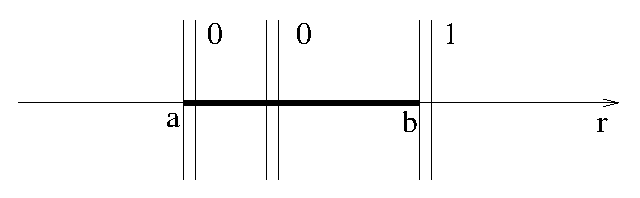
\includegraphics{./Euler-figs/morse1d}
  \caption{Schnittrekursion in einer Dimension. Nur der Punkt $r=b$ liefert einen Beitrag.}
  \label{fig:morse1d}
\end{figure}
Die Euler-Charakteristik einer eindimensionalen Figur ist daher die Zahl der Komponenten der Figur.  
\\In zwei Dimensionen sind kritische Punkte von $h_{\mathbf{n}}$ nach oben oder unten ausgerichtete Kuppen oder Mulden (siehe Abb. \ref{fig:2dschnitt}). Bei nach unten ausgerichteten Mulden oder Kuppen \"andert sich die $\chi(E_{r}\cap X)$ nicht, bei nach oben ausgerichteten Kuppen ist $\chi(E_{r_c}\cap X)-\lim_{\epsilon \rightarrow 0}\chi(E_{r_c+\epsilon}\cap X)=1$ und bei nach oben ausgerichteten Mulden ist $\chi(E_{r_c}\cap X)-\lim_{\epsilon \rightarrow 0}\chi(E_{r_c+\epsilon}\cap X)=-1$. F\"ur den \"au"seren Rand ergibt sich dadurch ein Beitrag $+1$, f\"ur alle inneren R\"ander $-1$. 
In zwei Dimensionen ist $\chi(X)$ also die Zahl der Komponenten von $X$, abz\"uglich der Zahl der L\"ocher in diesen Komponenten.
\begin{figure}[htbp]
  \centering
  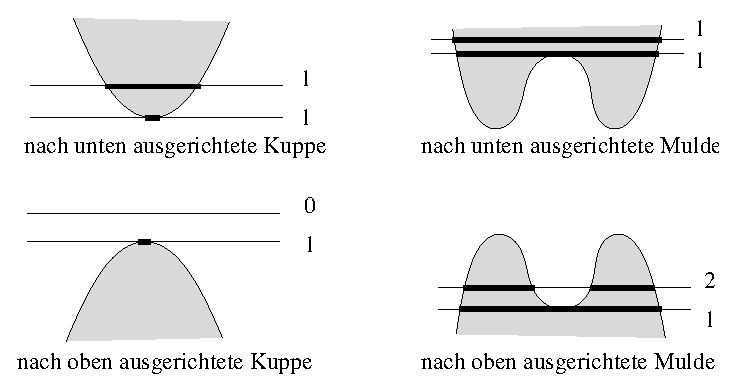
\includegraphics{./Euler-figs/2dschnitt}
  \caption{Schnittrekursion in zwei Dimensionen.}
  \label{fig:2dschnitt}
\end{figure}
\\In drei Dimensionen muss zwischen Maxima, Minima und Sattelpunkten unterschieden werden. Man \"uberlegt sich einfach, dass Maxima und Minima in bestimmten Orientierungen einen Beitrag $+1$ liefern, w\"ahrend Sattelpunkte $-1$ beitragen. Die Euler-Charakteristik in drei Dimensionen ist daher die Zahl der Komponenten, abz\"uglich der Zahl der Tunnel oder Henkel, plus der Zahl der Einschl\"usse.\\
Die Punkte, an denen sich $\chi(E_{r}\cap X)$ \"andert, lassen sich auch ohne eine differenzierbare H\"ohenfunktion angeben, und ein glatter Rand von $K$ ist f\"ur die Anwendbarkeit der Schnittrekursion nicht notwendig. Deshalb ist die Schnittrekursion f\"ur die Anwendung auf Gittern besonders geeignet.

\section{Euler-Charakteristik in der Graphentheorie}
\label{sec:graphen}
Hier sollen einige Begriffe der Graphentheorie erw\"ahnt werden, auf die im weiteren Verlauf zur\"uckgegriffen wird. Eine umfangreiche Sammlung von Definitionen der Begriffe der Graphentheorie ist in \cite{Essam:70} zu finden. \\
Ein \textit{Graph} $G$ besteht aus einer Vertexmenge $V$ und einer Kantenmenge $E$, die ungeordnete Paare von Vertices enth\"alt. Jedes Element $xy\in E$ ist und entspricht einer Verbindung der Vertices $x,y\in V$. Ein \textit{Subgraph} $G'$ besteht aus einer Teilmenge der Vertices $V'\subset V$ und einer Teilmenge der Kanten $E' \subset E$ von $G$, wobei $E'$ nur Paare von Vertices enthalten darf, die beide in $V'$ sind. Ein Graph heisst zusammenh\"angend, wenn es zu je zwei Vertices $x,y\in V$ eine Folge von Kanten $xz_1,z_1y_2,\ldots,z_ny$ gibt, die $x$ und $y$ verbindet. Ein zusammenh\"angender maximaler Subgraph hei"st Komponente von $G$. Mit der Zahl der Komponenten $n(G)$, der Zahl der Vertices $|V|$ und der Zahl der Kanten $|E|$ wird die \textit{zyklomatische Zahl} $z(G)$ eines Graphen $G$ durch
\begin{equation}
  z(G):=|E|-|V|+n(G)
\end{equation}
definiert. Ein Graph hei"st \textit{planar}, wenn es m\"oglich ist, ihn in die Ebene zu zeichnen, ohne dass sich zwei Kanten schneiden. Ein in die Ebene eingebetteter planarer Graph zerscheidet die Ebene in endliche Gebiete. Diese endlichen Gebiete entsprechen den Fl\"achen einer ebenen Figur aus Fl\"achen, Kanten und Ecken. Da die Euler-Charakteristik einer ebenen Figur aus $n$ Komponenten den Wert $n$ hat, folgt aus dem Eulerschen Satz, dass die Zahl der endlichen Gebiete gleich der zyklomatischen Zahl $z(G)$ ist \cite{Essam:70}. Wenn $G$ der Graph eines zweidimensionalen planaren Gitters ist, nennen wir die endlichen Gebiete \textit{Plaketten} des Gitters. 
\\Eine Graph heisst \textit{bibartit}, wenn die Vertexmenge $V$ die disjunkte Vereinigung zweier Mengen $V_1$ und $V_2$ ist, so dass jede Kante $v_1v_2\in E$ einen Vertex aus $v_1\in V_1$ mit einem Vertex $v_2 \in V_2$ verbindet.



\section{Euler-Charakteristik auf Gittern}
\label{sec:chimittel}
In dieser Arbeit wird die mittlere Euler-Charakteristik von diversen Perkolationskonfigurationen auf Gittern berechnet. Um eine sinnvolle Definition der Euler-Charakteristik f"ur Perkolationskonfigurationen zu erhalten, muss das geometrische Objekt, das mit einem Gittercluster identifiziert werden soll, festgelegt werden. Jeder Cluster, der alle Gitterpunkte innerhalb einer konvexen H"ulle enth"alt, sollte Euler-Charakteristik 1 haben; L\"ocher sollten nur in Verbindung mit unbesetzten Vertices auftreten. Man muss daher zu jedem Vertex eine Zelle finden, so dass die Vereinigung aller Zellen raumf\"ullend ist, und die durch Vereinigung mancher Zellen entstehenden Figuren die Topologie der entsprechenden Gittercluster haben.  
\subsection{Zweidimensionale Gitter}
\label{sec:chimittel2d}
In zwei Dimensionen wird nat"urlicherweise die Vereinigung der dualen Plaketten der besetzten Vertices mit den Gitterclustern identifiziert. Die dualen Plaketten zweier benachbarter Vertices teilen eine gemeinsame Kante und sind dadurch verbunden. Aber auch alle dualen Plaketten der Vertices auf dem Rand einer Gitterplakette haben den dualen Vertex dieser Plakette gemein (siehe Abb. \ref{fig:decoratedtopo}). 
\begin{figure}[htbp]
  \centering
  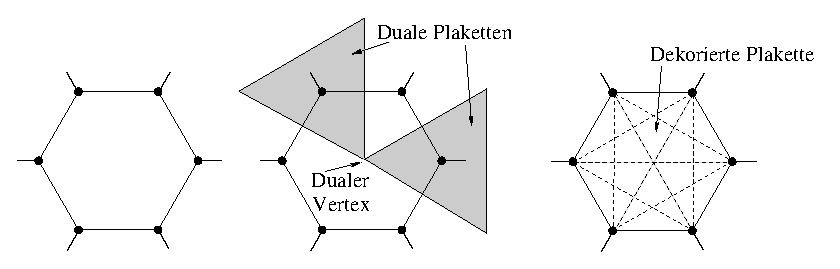
\includegraphics{./Euler-figs/decoratedtopo}
  \caption{Links ist eine Plakette des Sechseckgitters gezeigt. In der Mitte sind zwei duale Plaketten eingezeichnet, deren Vertices nicht benachbart sind. Diese Plaketten ber\"uhren sich am dualen Vertex des Sechseckes. Rechts ist das dekorierte Sechseck mit allen diagonalen Verbindungen dargestellt.  }
  \label{fig:decoratedtopo}
\end{figure}
Im Allgemeinen sind diese Vertices aber nicht benachbart, und die Muster, die entstehen, wenn duale Plaketten besetzt werden, haben nicht die Gittertopologie. Diese Zusammenhangsverh\"altnisse entsprechen einem Gitter, bei dem alle Vertices auf dem Rand einer Plakette miteinander verbunden sind. Ein solches Gitter heisst vollst\"andig dekoriertes Gitter.
In aller Regel wird Perkolation aber auf undekorierten Gittern behandelt. Die Euler-Charakteristik des undekorierten Gitters erh\"alt man \"uber den Umweg, statt den besetzten die unbesetzten Vertices mit dualen Plaketten zu belegen, und die Euler-Charakteristik des unbelegten Komplements zu berechnen (siehe Abb. \ref{fig:dualplaqu}). 
\begin{figure}[bp]
  \centering
  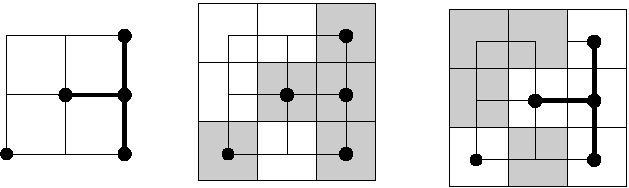
\includegraphics{./Euler-figs/dualplaqu}
  \caption{Links sind zwei Cluster auf dem Quadratgitter dargestellt. Setzt man auf jeden besetzten Vertex ein duales Quadrat (Mitte) entsteht eine zusammenh\"angende Figur. Besetzt man stattdessen die unbesetzten Vertices (rechts), zerf\"allt das Komplement in Komponenten, die den Clustern entsprechen. }
  \label{fig:dualplaqu}
\end{figure} 
Man berechnet zuerst $\chi(\bar{X})$ des Musters $\bar{X}$, das von den Plaketten auf unbesetzten Vertices gebildet wird. Die Vereinigung von $\bar{X}$ mit seinem Komplement $\check{X}$ ist die komplette Ebene, und die Summe der Euler-Charakteristiken von $\bar{X}$ und $\check{X}$ ist $1$ \cite{Saskin:89}. Die Euler-Charakteristik der offenen Menge $\check{X}$ ist daher $\chi(\check{X})=1-\chi(\bar{X})$. Wir wollen aber mit abgeschlossenen Mengen arbeiten und m\"ussen daher $\check{X}$ mit einem geeigneten Abschluss vereinigen. Der Rand $\partial \bar{X}$ von $\bar{X}$ ist ungeeignet, da er aus Kurven besteht, die sich selbst schneiden. Die Kurven w\"urden verschiedene Komponenten des Komplements miteinander verbinden und dadurch seine Zusammenhangsverh\"altnisse ver\"andern. Durch Modifikation der punktf\"ormigen \"Uberlappungen der Plaketten in $\bar{X}$, k\"onnen solche Kurven aber vermieden werden, ohne $\chi(\bar{X})$ zu ver\"andern (siehe Abb. \ref{fig:mod}).
\begin{figure}[htbp]
  \centering
  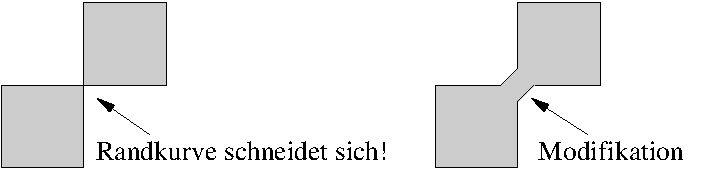
\includegraphics{./Euler-figs/mod}
  \caption{Notwendige Modifikation am Beispiel des Quadratgitters.}
  \label{fig:mod}
\end{figure}
Nachdem diese Modifikationen an $\bar{X}$ (und an $\check{X}$) durchgef\"uhrt worden sind, besteht der Rand $\partial \bar{X}$ nur noch aus geschlossenen einfachen Kurven, deren Euler-Charakteristik verschwindet. Die Euler-Charakteristik von $X=\check{X}\cup\partial \bar{X}$ ist also $\chi(X)=\chi(\check{X})=1-\chi(\bar{X})$.
\\Um die mittlere Euler-Charakteristik der Cluster, die durch Besetzten der Vertices eines undekorierten Gitters mit Wahrscheinlichkeit $p$ entstehen, zu berechnen, setzt man auf die Vertices eines Gitterausschnitts mit Wahrscheinlichkeit $q=1-p$ duale Plaketten und bestimmt die mittlere Euler-Charakteristik $\left<\chi(\bar{X})\right>_q$ dieser Muster $\bar{X}$. Die mittlere Euler-Charakteristik pro Vertex ist $\bar{\chi}(q):=\frac{1}{|V|}\left<\chi(\bar{X})\right>_q$, wobei $|V|$ die Zahl der Vertices im betrachteten Gitterausschnitt ist. Randterme verschwinden im Limes gro"ser Gitterausschnitte \cite{Jung:00}. F\"ur die Euler-Charakteristik des undekorierten Gitters erh\"alt man $\chi(p)=-\bar{\chi}(q)$; der Term $\frac{1}{|V|}$ verschwindet f\"ur $|V|\rightarrow \infty$. $\chi(p)$ und $\bar{\chi}(q)$ sind die Euler-Charakteristiken eines komplement\"ar besetzten Paares von matching-Gittern (siehe Abb. \ref{fig:chi}). Da die mittlere Euler-Charakteristik zweidimensionaler Gitter zwischen $0$ und $1$ nur eine Nullstelle hat \cite{Wagner:02}, ist die Nullstelle des self-matching Dreiecksgitters $p_0=\frac{1}{2}$ und f\"allt mit der Perkolationsschwelle zusammen. Die matching-Eigenschaft $\chi(p)=-\bar{\chi}(q)$ gilt nicht nur f\"ur planare Gitter, sondern auch f\"ur beliebige dekorierte Mosaike (siehe Abschnitt \ref{sec:matchingpoly}). F\"ur jedes self-matching Gitter gilt damit $p_0=p_c=\frac{1}{2}$. Wenn im Folgenden von der Euler-Charakteristik eines Gitters die Rede ist, sei die mittlere Euler-Charakteristik pro Vertex der Cluster verstanden, die beim Besetzen der Gittervertices mit Wahrscheinlichkeit $p$ entstehen. 
\begin{figure}[bp]
  \centering
  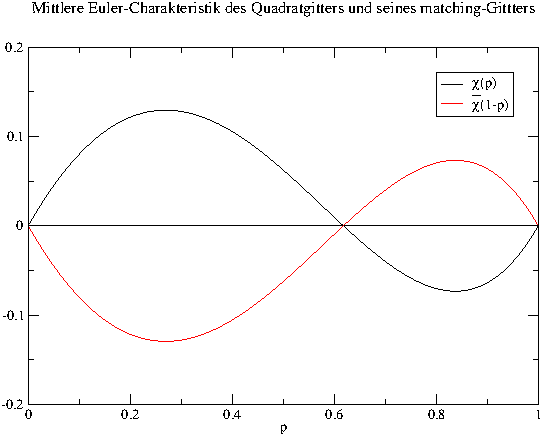
\includegraphics[width=10cm]{./Euler-figs/chi_fig}
  \caption{Mittlere Euler-Charakteristik des Quadratgitters und seines komplement\"ar besetzten matching-Gitters. Siehe Gleichung (\ref{eq:chisquare}).}
  \label{fig:chi}
\end{figure}
\\Am Beispiel des Quadratgitters mit Besetzungswahrscheinlichkeit $p$ soll hier die Berechnung von $\chi(p)$ mit den unterschiedlichen Methoden vorgef\"uhrt werden. Alle Gitterpl\"atze werden mit Wahrscheinlichkeit $q=1-p$ mit einem dualen Quadrat belegt. Wir berechnen also $\bar{\chi}(q)$ des mit Wahrscheinlichkeit $q$ besetzten matching-Gitters und erhalten durch $\chi(p)=-\bar{\chi}(1-p)$ die Euler-Charakteristik des Quadratgitters. Die Berechnung kann mit der Schnittrekursion oder durch Berechnung der Beitr\"age disjunkter randloser Zellen erfolgen.\\
Die \textbf{Schnittrekursion} ist mit jeder beliebig ausgerichteten Geradenschar $E_r$ m\"oglich. Die Euler-Charakteristiken der Schnitte mit den Geraden bezeichen wir mit $\chi^1(q)$. Zun\"achst w\"ahlen wir eine Schar $E_x$ parallel zu einer der Gitterrichtungen. Das Schnittmuster der Geraden mit den belegten Quadraten kann sich nur "andern, wenn die Gerade von einer Reihe Quadrate in die n\"achste wechselt (siehe Abb. \ref{fig:schnittquadrat}). Die kritischen Werte von $x$ liegen daher dort, wo duale Quadrate sich ber\"uhren.  
\begin{figure}[hbtp]
  \centering
  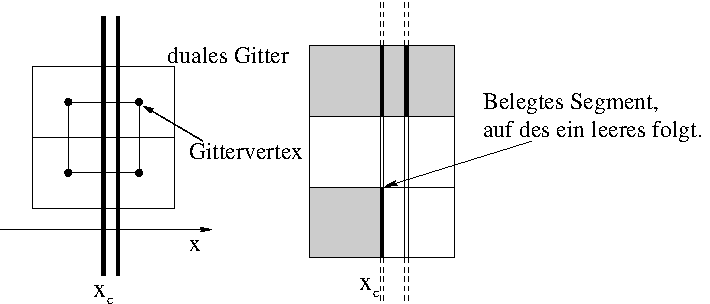
\includegraphics{./Euler-figs/schnittquadrat}
  \caption{Schnittrekursion beim Quadratgitter. Kritische Werte von $x$ liegen dort, wo sich duale Quadrate ber\"uhren. Im rechten Teil der Abbildung sind verschiedene Anordnungen und die resultierenden Schnittmuster auf den Geraden gezeigt.}
  \label{fig:schnittquadrat}
\end{figure}
\\Ein Segment der Geraden, also eine Kante des dualen Gitters, ist an kritschen Werten von $x=x_c$ belegt, wenn mindestens eines der angrenzenden Quadrate belegt ist. Die Zahl der Komponenten des Schnittmusters ist gleich der Zahl der belegten Segmente, auf die ein leeres Segment folgt. Die mittlere Euler-Charakteristik einer Gerade bei $x=x_c$, normiert auf die L\"ange, ist also $\chi^1_{x_c}(q)=(1-(1-q)^2)(1-q)^2$. Entsprechend ist f\"ur eine Gerade bei unkritischem $x$ die Euler-Charakteristik gleich $\chi^1_{x}=q(1-q)$. Die Differenz ergibt 
\begin{equation}
\label{eq:chisquare}
\bar{\chi}(q)=(1-(1-q)^2)(1-q)^2-(1-q)q=q-4q^2+4q^3-q^4,
\end{equation} 
und daher ist die mittlere Euler-Charakteristik des Quadratgitters $\chi(p)=-\bar{\chi}(1-p)=p-2p^2+p^4$.\\
Nun betrachten wir eine Schar von Geraden $E_r$, die zu keiner dualen Gitterkante parallel sind. Die Vertices des dualen Gitters entsprechen den kritischen Punkten und wir berechnen die erwartete \"Anderung von $\chi^1_{r_c}(q)$ in einer Umgebung des Vertex. In Abb. \ref{fig:morsequadrat} sind die einzigen beiden Konfigurationen gezeigt, bei denen sich $\chi^1_{r_c}(q)$ beim \"Uberstreichen des Vertex in Pfeilrichtung \"andert. Im ersten Fall betr\"agt die \"Anderung $-1$, und diese Konfiguration hat die Wahrscheinlichkeit $qp^3$. Im zweiten Fall ist die \"Anderung $+1$, und die Konfiguration hat Wahrscheinlichkeit $q^2p$. Es ergibt sich 
\begin{equation}
\bar{\chi}(q)=q(1-q)^3-q^2(1-q)=q-4q^2+4q^3-q^4
\end{equation} 
und damit $\chi(p)=-\bar{\chi}(1-p)=p-2p^2+p^4$.
Bei Verwendung dieser Geradenschar sieht man sehr gut, wie der Erwartungswert der Euler-Charakteristik durch lokale Beitr\"age der einzelnen Vertices zustande kommt, und wie sich unterschiedlichen Zusammenhangsverh\"altnisse des planaren und vollst\"andig dekorierten Gitters auf die Euler-Charakteristik auswirken.
\begin{figure}[hbtp]
  \centering
  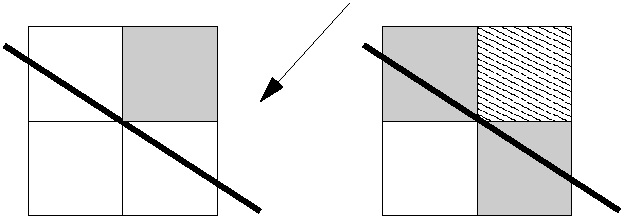
\includegraphics{./Euler-figs/morsequadrat}
  \caption{Die beiden Konfigurationen des Quadratgitters, die zur Schnittrekursion mit den eingezeichneten Geraden in Pfeilrichtung beitragen. Grau gezeichnete Quadrate sind besetzt, wei"se unbesetzt. Die linke Konfiguration hat Wahrscheinlichkeit $q(1-q)^3$ und tr\"agt $+1$ bei, die rechte hat Wahrscheinlichkeit $q^2(1-q)$ und tr\"agt $-1$ bei. Der Zustand des schraffierten Quadrates ist f\"ur die \"Anderung von $\chi^1_{r_c}(q)$ unerheblich.}
  \label{fig:morsequadrat}
\end{figure}
\\Eine andere, h\"aufig zweckm\"a"sigere, Methode, die Mittelwerte auszurechnen, besteht darin, das duale Gitter in \textbf{disjunkte Zellen} zu zerlegen und die erwartete Anzahl derjenigen Zellen zu bestimmen, die durch Belegen mit dualen Plaketten bedeckt werden \cite{Likos:95}. Die disjunkten Zellen sind die Plaketten ohne Rand, die Kanten ohne Endpunkte und die Vertices des dualen Gitters. 
\begin{itemize}
\item Plaketten sind mit Wahrscheinlichkeit $q$ belegt und auf ihre Gesamtzahl $|V|$ wird normiert. 
\item Duale Kanten sind bedeckt, wenn mindestens eine der angrenzenden Plaketten belegt ist; die Wahrscheinlichkeit daf\"ur ist $(1-(1-q)^2)=1-p^2$. Jede duale Kante entspricht einer Kante des urspr\"unglichen Gitters. Daher ist die Zahl der dualen Kanten pro dualer Plakette gleich der Zahl der Kanten pro Vertex. Sie betr\"agt $\frac{z}{2}$, denn jede Kante endet an 2 Vertices, und von jedem Vertex gehen $z$ Kanten aus.
\item Ein dualer Vertex ist in allen $n$ umgebenden dualen Plaketten enthalten und daher mit Wahrscheinlichkeit $(1-(1-q)^n)=1-p^n$ pr\"asent. $n$ ist die Kantenzahl der Plakette des urspr\"unglichen Gitters, in der der duale Vertex sitzt.
\end{itemize}
F\"ur das Quadratgitter ist $z=4$ und die Zahl der Quadrate ist gleich der Zahl der Vertices. Man erh\"alt wie oben 
\begin{equation}
\bar{\chi}(q)=q-2(1-(1-q)^2)+(1-(1-q)^4)=q-4q^2+4q^3-q^4
\end{equation} 
und damit $\chi(p)=p-2p^2+p^4$.\\

Die mittlere Koordinationszahl eines Gitters ist \"uber den Euler'schen Satz durch die Zahl der Plaketten bestimmt, und alle Kanten sind bei Besetzung der dualen Plaketten mit der gleichen Wahrscheinlichkeit $1-p^2$ vorhanden. Daher h\"angt die mittlere Euler-Charakteristik eines planaren zweidimensionalen Gitter ausschlie"slich von der Anzahl seiner Plaketten und deren Kantenzahl ab.\\

\subsubsection{Gittertiere}
In zwei Dimensionen ist die Euler-Charakteristik einer Gitterkonfiguration die Differenz der Anzahl der Cluster und der Anzahl der L\"ocher in diesen Clustern. Nach Konstruktion ist jedes Loch ein Cluster des komplement\"ar besetzten matching-Gitters. Die Zahl der Cluster pro Vertex auf dem mit Wahrscheinlichkeit $p$ besetzten Gitter ist $n(p)$; die Zahl Cluster pro Vertex des mit Wahrscheinlichkeit $q=1-p$ besetzten matching-Gitter ist $n^*(q)$. Die mittlere Euler-Charakteristik des Gitters ist also die Differenz von $n(p)$ und $n^*(q)$. Im Abschnitt \ref{sec:animals} wurde die Zahl der Cluster pro Vertex durch eine Summe \"uber alle m\"oglichen endlichen Cluster, die sog. Gittertiere oder lattice animals, ausgedr\"uckt. Mit den Anzahlen der m\"oglichen Cluster $g_{st}$ bzw. $g^*_{st}$ der Masse $s$ und Umfang $t$ auf den beiden Gittern erh\"alt man 
\begin{equation}
n(p)=\sum_{s,t}g_{st}p^sq^t \qquad \text{und} \qquad n^*(q)=\sum_{s,t}g^*_{st}q^sp^t.
\end{equation}  
Der unendliche Cluster spielt hier keine Rolle, denn der Beitrag eines einzigen Clusters zur Zahl der Cluster pro Vertex verschwindet. 
Die mittlere Euler-Charakteristik ist damit
\begin{equation}
  \label{eq:chianimals}
  \chi(p)=\sum_{s,t} \left(g_{st}p^sq^t-g^*_{st}q^sp^t\right).
\end{equation}
Die ersten Cluster, die zu diesen Reihen beitragen, sind f\"ur den Fall des Quadratgitters in Abbildung \ref{fig:animals} dargestellt. Die $\chi(p)$ ist also die Differenz zweier unendlicher Polynome. Andererseits l\"asst sich $\chi(p)$ lokal ausrechnen und ist ein Polynom endlicher (kleiner) Ordnung. Die Terme in Gl. (\ref{eq:chianimals}) m\"ussen sich also bis auf einige wenige wegheben \cite{Sykes:64}.
\begin{figure}[tbp]
  \centering
  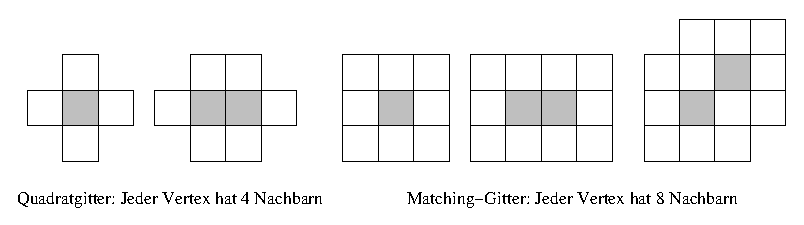
\includegraphics{./Euler-figs/animals}
  \caption{Gittertiere bis zur Gr\"o"se $s=2$ auf dem Quadratgitter (links) und auf dem machting-Gitter (rechts) mit $t=4$ und $t=6$ bzw. $t=8$, $t=10$ und $t=12$. Es ist jeweils nur eine Orientierung der Gittertiere dargestellt.}
  \label{fig:animals}
\end{figure}
Die Zahl $g_{st}$ steigt mit $s$ und $t$ schnell an, und wurde f\"ur das Quadratgitter bis $s = 22$ und $t=46$ von Mertens \cite{Mertens:90} mit Hilfe von Computern abgez\"ahlt. 
Auf dem Quadratgitter kommen die Terme, die zu $\chi(p)$ beitragen, ausschlie"slich von $n(p)$, da $n^*(q)$ als Polynom in $p$ erst mit $p^8$ beginnt:
\begin{equation}
  \begin{split}
  \chi(p)&=pq^4+2p^2q^6+p^3(4q^6+2q^7)+p^4(9q^8+8q^9+2q^{10})+\cdots\\
&-qp^8-q^2(2p^{10}+2p^{12})-\cdots\\
 &=p-2p^2+p^4.
  \end{split}
\end{equation}


\subsubsection{Euler-Charakteristik dekorierter Mosaike}
\label{sec:matchingpoly}
Fortuin und Kastelyn haben 1972 in einer Serie von Arbeiten \cite{Fortuin:72} das Random-Cluster-Modell vorgestellt und gezeigt, dass bond-Perkolation dem Limes $\lambda \rightarrow 1$ eines Potts-Modells, dessen Spins $\lambda$ verschiedene Zust\"ande annehmen k\"onnen, entspricht. Essam \cite{Essam:79} hat diese Korrespondenz durch Einf\"uhrung von Wechselwirkungen, an denen mehrere Spins teilnehmen, auf site-Perkolation erweitert. Die Dualit\"at der Hoch- und Tieftemperaturzustandssumme zweidimensionaler Pottsmodelle entspricht im Limes $\lambda \rightarrow 1$ der matching-Eigenschaft der site-Perkolation. Das matching-Polynom, das Essam einf\"uhrt, ist die mittlere Euler-Charakteristik des assoziierten Perkolationsproblems. Der Wechselwirkungsgraph des Pottsmodells aus \cite{Essam:79} l\"asst sich f\"ur jedes dekorierte Mosaik konstruieren, so dass die mittlere Euler-Charakteristik eines site-Perkolationsproblems auf beliebig dekorierten Mosaiken berechnet werden kann. Die folgende Konstruktion ist so zu verstehen, dass sie zun\"achst auf einem endlichen Gitterausschnitt durchgef\"uhrt wird. Anschlie"send muss der Limes zu unendlichen Gittern in geeigneter Weise durchgef\"uhrt werden \cite{Essam:79}. \\
Der Wechselwirkungsgraph setzt sich aus Spinvertices $s\in S$ und Wechselwirkungsvertices $i\in I$ zusammen. Um den Wechselwirkungsgraph eines Perkolationsproblems auf einem dekorierten Mosaik zu erhalten, werden Spins auf alle Kanten und in alle dekorierten Plaketten des Mosaiks gesetzt. Die Wechselwirkungsvertices sitzen auf den Ecken des Mosaiks (siehe Abb. \ref{fig:interactiongraph}).
\begin{figure}[tbp]
  \centering
  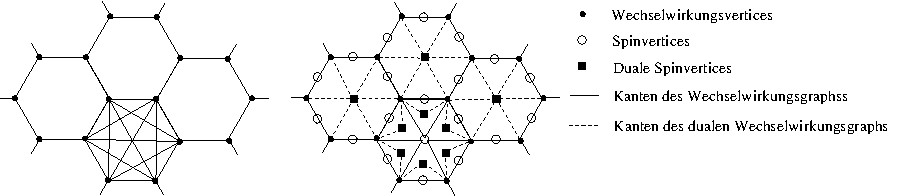
\includegraphics{./Euler-figs/interactiongraph}
  \caption{Ausschnitt aus einem dekorierten Mosaik (links) und die resultierenden Wechselwirkungsgraphen (rechts).}
  \label{fig:interactiongraph}
\end{figure}
Ein Wechselwirkungsvertex $i$ vermittelt eine Wechselwirkung zwischen allen Spins auf den Kanten und in den Plaketten, die diesen Vertex umgeben. Jeder Wechselwirkungsvertex $i$ wird mit allen Spinvertices verbunden, die in $i$ wechselwirken. Dadurch entsteht ein bipartiter, planarer und zusammenh\"angender Graph $G$. Zu diesem Graphen wird ein ein dualer Wechselwirkungsgraph $G^*$ konstruiert, dessen Vertexmenge aus dualen Spinvertices $s^* \in S^*$ und den Wechselwirkungsvertices $i\in I$ besteht. Die dualen Spinvertices $s^* \in S^*$ werden in alle Plaketten von $G$ gesetzt, und jeder Wechselwirkungsvertices wird mit allen umgebenden dualen Spins verbunden (siehe Abb. \ref{fig:interactiongraph}).
\\Wir betrachten nun den Subgraph $G=(V,E)$ mit Vertexmenge $V=S\cup I'$, $I'\subset I$, und den Subgraph $G^*=(V^*,E^*)$ mit Vertexmenge $V^*=S^*\cup I\backslash I'$. Die Kantenmengen der Subgraphen bestehen aus allen Kanten, deren Endvertices beide in $V$ bzw. $V^*$ sind. Bettet man beide Graphen in die Ebene ein, ist jede endliche Komponente von $G$ in einer Plakette von $G^*$ enthalten; gleiches gilt umgekehrt \cite{Essam:79}. Die Differenz der Komponenten $n(G)$ und $n^*(G^*)$ von $G$ bzw. $G^*$ ist nach dem Euler'schen Satz 
\begin{equation}
  n(G)-n^*(G^*)=|V|-|E|-1
\end{equation}
Der Term $-1$ entspricht der unendlichen Komponente. W\"ahlt man Vertices $I'$ aus $I$ mit Wahrscheinlichkeit $p$ aus und mittelt \"uber alle Konfigurationen, erh\"alt man die mittlere Euler-Charakteristik. Komponenten, die nur aus isolierten Spins bestehen, entsprechen keinen Clustern oder L\"ochern des Perkolationsproblems auf dem dekorierten Mosaik und m\"ussen daher noch abgezogen werden (Summen \"uber $S$ und $S^*$ in Gl. (\ref{eq:matchingpoly})). Das Resultat ist das matching-Polynom \cite{Essam:79} oder die mittlere Euler-Charakteristik:
\begin{equation}
  \chi(p)=|S|+\sum_{i\in I} p-\sum_{i\in I} z_i p-1 -\sum_{s \in S}(1-p)^{z_s}+\sum_{s^* \in S^*}p^{z_{s^*}}.
  \label{eq:matchingpoly}
\end{equation}
$z_v$ ist die Koordinationszahl des Vertex $v$. Um $\chi(p)$ zu normieren, muss noch durch $|I|$ geteilt werden. Da $G$ ein zusammenh\"angender Graph ist, gilt nach dem Euler'schen Satz $v-e+f=|S|+|I|-\sum_{i\in I}z_i +|S^*|=2$ (die unendliche Plakette mitgez\"ahlt) und damit die matching-Relation $\chi(p)=-\chi^*(1-p)$ f\"ur beliebige komplement\"ar dekorierte Mosaike.
\\F\"ur planare und vollst\"andig dekorierte Gitter stimmen die mit Gleichung (\ref{eq:matchingpoly}) berechneten Euler-Charakteristiken mit den Ergebnissen, die mit den anderen Methoden erhalten werden, \"uberein. Man \"uberzeugt sich leicht, dass die einzelnen Terme aus (\ref{eq:matchingpoly}) in diesen F\"allen den Beitr\"agen der Plaketten, Kanten und Ecken entsprechen. 

\subsection{Dreidimensionale Gitter}
Im vorigen Abschnitt haben wir gesehen, dass die Vereinigung dualer Zellen eines zweidimensionalen Gitters die topologischen Eigenschaften des vollst\"andig dekorierten Gitters hat. Das Komplement hat die Zusammenhangsverh\"altnisse des undekorierten Gitters.\\
Entsprechendes gilt unter bestimmten Voraussetzungen f\"ur dreidimensionale Gitter. Wir betrachten ein Gitter und raumf\"ullende Zellen um die Vertices, z.B. W\"urfel um die Vertices des einfach-kubischen Gitters (sc-Gitter). Die Vereinigung dieser Zellen hat die topologischen Eigenschaften eines Gitters, dessen Vertices miteinander verbunden sind, wenn ihre Zellen einen nichtleeren Durchschnitt haben. Beim sc-Gitter sind das alle W\"urfel, die eine Ecke, Kante oder Fl\"ache teilen, und jeder Vertex h\"atte 26 Nachbarn. Vertices des Gitter haben aber in der Regel sehr viel weniger Nachbarn; das sc-Gitter beispielweise nur sechs. Wenn die und nur die Zellen, deren Vertices Gitternachbarn sind, einen Durchschnitt haben der nur in diesen beiden Zellen enthalten ist, hat das Komplement die topologischen Eigenschaften des Gitters. Das sc-Gitter erf\"ullt diese Voraussetzung, denn Kanten sind in vier und Ecken in acht W\"urfeln enthalten, w\"ahrend die Fl\"achen nur zu zwei W\"urfeln geh\"oren und den Gitterkanten entsprechen. 
\\Um zu einem Vertex eine Zelle zu konstruieren, betrachtet man die Ebenen senkrecht auf der Mitte der Verbindungslinien zu den n\"achsten, \"ubern\"achsten, usw. Gitternachbarn. Jede dieser Ebenen definiert einen Halbraum, der den Vertex enth\"alt. Die Wigner-Seitz-Zelle (WSZ) eines Gittervertex ist der Durchschnitt aller so konstruierten Halbr\"aume. Die WSZ der Bravais-Gitter sind raumf\"ullend. Wenn jede Fl\"ache der WSZ einer Gitterkante entspricht und die WSZ raumf\"ullend sind, sind die WSZ geeignet, um die Euler-Charakteristik zu bestimmen. Bei manchen Gittern, z.B. dem bcc-Gitter, haben die WSZ aber mehr Fl\"achen als Gitternachbarn.
\\F\"ur Gitter, die keine Bravaisgitter sind, oder deren WSZ zu viele Fl\"achen haben, kann man dennoch geeignete raumf\"ullende Zellen finden. Diese sind aber h\"aufig nicht konvex. Der Durchschnitt zweier Gitternachbarn besteht dann aus verschiedenen Fl\"achenst\"ucken, inklusive den zwischen diesen St\"ucken liegenden Kanten (siehe Abb. \ref{fig:bcc_nonconvex_app}). 
\\Ob der Durchschnitt der Gitternachbarn eben ist oder nicht, spielt keine Rolle; wichtig ist nur, dass der Durchschnitt der Zellen zweier Gitternachbarn, abgesehen von den Randkanten, nur in diesen Zellen enthalten ist, und dass der Durchschnitt aller \"ubrigen Zellen in mehr als zwei Zellen enthalten ist. Dadurch wird gew\"ahrleistet, dass unbesetzte Zellen, die keine Gitternachbarn sind, durch besetzte Zellen getrennt werden, und dass eben dies bei Gitternachbarn nicht geschieht.
\\Hat man geeignete Zellen gefunden, werden die Zellen, die unbesetzten Vertices entsprechen, ausgew\"ahlt, und die Euler-Charakteristik der entstehenden Figur $\bar{X}$ ausgerechnet. Die Euler-Charakteristik des Komplements $\check{X}$ ist $\chi(\check{X})=-\chi(\bar{X})+\mathcal{O}(1)$; $\check{X}$ ist aber eine offene Menge. Damit der Rand $\partial \bar{X}$ ein geeigneter Abschluss von $\check{X}$ ist, muss im dreidimensionalen Fall $\bar{X}$ \"uberall dort modifiziert werden, wo Zellen nur an Ecken oder Kanten \"uberlappen. Die Euler-Charakteristik $\chi(\bar{X})$ bleibt bei diesen Modifikationen unver\"andert. Die Euler-Charakteristik des Randes nach der Modifikation ist nach Gleichung (\ref{eq:opensets}) $\chi(\partial \bar{X})=2\chi(\bar{X})$. Damit erh\"alt man f\"ur der Euler-Charakteristik der Vereinigung $X$ von $\check{X}$ (entsprechend modifiziert) mit $\partial \bar{X}$ 
\begin{equation}
  \chi(X)=\chi(\check{X})+\chi(\partial \bar{X})=-\chi(\bar{X})+2\chi(\bar{X})+\mathcal{O}(1)=\chi(\bar{X})+\mathcal{O}(1)
\end{equation}
Uns interessiert hier die mittlere Euler-Charakteristik pro Vertex $\chi(p)$ der Muster, die bei site-Perkolation mit Besetzungswahrscheinlichkeit $p$ entstehen. Die Euler-Charakteristik $\chi(p)$ ist gleich der des Komplements $\bar{\chi}(1-p)$. Wie in zwei Dimensionen verschwinden m\"ogliche Randterme im Limes gro"ser Gitter \cite{Jung:00}. Am Beispiel des sc-Gitter werden zwei Methoden, $\chi(p)$ zuberechnen, vorgestellt.
\\Die mittlere Euler-Charakteristik des sc-Gitters l\"asst sich einfach mit der \textbf{Schnittrekursion} und einem Satz von Ebenen, die parallel zu den Gitterebenen sind, bestimmen. Das Schnittmuster der Ebene mit den besetzten W\"urfeln, ist ein Muster aus Quadraten eines Quadratgitters. Die Muster \"andern sich, wenn die Ebene von einer Schicht W\"urfel in die n\"achste wandert. Zwischen zwei Schichten von W\"urfeln sind die Quadrate des Schnittmusters belegt, wenn mindestens einer der angrenzenden W\"urfel besetzt ist. Das Schnittmuster hat daher die Euler-Charakteristik eines mit Wahrscheinlichkeit $1-(1-q)^2$ besetzten, vollst\"andig dekorierten Quadratgitters $\bar{\chi}^{Qu}(1-(1-q)^2)$. Schnittmuster der Ebenen, die nicht zwischen zwei Schichten von W\"urfeln liegen sind entsprechend mit Wahrscheinlichkeit $q$ belegt und haben Euler-Charakteristik $\bar{\chi}^{Qu}(q)$. Ihre Differenz ist die Euler-Charakteristik des einfach-kubischen Gitters
\begin{equation}
\begin{split}
  \chi(p) & =\bar{\chi}(1-p)=\bar{\chi}^{Qu}(1-p^2)-\bar{\chi}^{Qu}(1-p)\\
&=p-3p^2+3p^4-p^8.
\end{split}
\end{equation}
\\Wenn ein Gitter keine einfache Schichtstruktur vorgibt, ist es zweckm\"a"siger $\bar{\chi}(q)$ aus den Beitr\"agen \textbf{disjunkter Zellen} zu berechnen \cite{Likos:95}. Dazu m\"ussen die Wahrscheinlichkeiten, dass die unterschiedlichen Zellen zur Figur geh\"oren, wenn abgeschlossene W\"urfel mit Wahrscheinlichkeit $q=1-p$ ausgew\"ahlt werden, bestimmt werden. 
\begin{itemize}
\item \textbf{W\"urfel} sind mit Wahrscheinlichkeit $q$ vorhanden. Jeder besetzte W\"urfel tr\"agt $-1$ bei.
\item Damit eine \textbf{Fl\"ache} zur Anordnung geh\"ort, muss mindestens einer der angrenzenden W\"urfel besetzt sein. Jede Fl\"ache ist also mit Wahrscheinlichkeit $1-(1-q)^2=1-p^2$ vorhanden. Ein W\"urfel hat sechs Fl\"achen, die je zu zwei W\"urfeln geh\"oren. Es gibt daher drei Fl\"achen pro W\"urfel, die $+1$ beitragen, wenn mindestens einer der angrenzenden W\"urfel besetzt ist.
\item Eine \textbf{Kante} ist Teil von vier W\"urfeln und daher mit Wahrscheinlichkeit $1-p^4$ pr\"asent. Ein W\"urfel hat zw\"olf Kanten, die aber je in vier W\"urfeln enthalten sind, und folglich gibt es drei Kanten pro W\"urfel. Eine Kante tr\"agt $-1$ zur Euler-Charakteristik bei.
\item Die \textbf{Ecke} eines W\"urfels ist auch Ecke von sieben anderen W\"urfeln und daher mit Wahrscheinlichkeit $1-p^8$ vorhanden. Pro W\"urfel gibt es eine Ecke, die, wen sie Teil der Anordnung ist, $+1$ beitr\"agt.
\end{itemize}
Summation der Beitr\"age liefert $\bar{\chi}(q)$ und damit auch $\chi(p)$:
\begin{equation}
  \chi(p)  =\bar{\chi}(1-p)=-(1-p)+3(1-p^2)-3(1-p^4)+1-p^8=p-3p^2+3p^4-p^8.
\end{equation}\\

Die Wahl der Zellen zur Berechnung der Euler-Charakteristik eines Gitters ist im Allgemeinen nicht eindeutig. Daher werden zur Unterscheidung unterschiedlicher Euler-Charakteristiken neben dem Namen des Gitters auch die Zahl $z$ der Fl\"achen einer Zelle, d.h. die Zahl der Gitternachbarn eines Vertex, und die Zahl $\bar{z}$ der Zellen, mit denen eine gegebene Zellen einen nichtleeren Durchschnitt hat, angegeben. Die Zahl $\bar{z}$ ist die Koordinationszahl eines Gitters, dessen Vertices verbunden sind, wenn die zugeh\"origen Zellen einen nichtleeren Durchschnitt haben. Dieses Gitter ist das Analogon eines vollst\"andig dekorierten Gitters in zwei Dimensionen. Anders als in zwei Dimensionen h\"angt es aber von der Wahl der Zellen ab. 
\\Ein Vertex des sc-Gitters hat sechs Nachbarn, und ein W\"urfel teilt mit 26 W\"urfeln eine Fl\"ache, Kante oder Ecke. F\"ur die mittlere Euler-Charakteristik des sc-Gitter schreiben wir somit $\chi^{sc}_{6-26}(p)$.
\\Die Berechnung der Euler-Charakteristik anderer Gitter und Gitter h\"oherer Dimensionen geht analog, ist aber h\"aufig um vieles aufwendiger.


  %17.09.03


\chapter{Stochastische Geometrie gemischter Perkolation}
\label{sec:mixed}

Im vorangehenden Kapitel wurden Methoden vorgestellt, mit denen die Euler-Charak\-teris\-tik von site-Perkolationsprozessen auf Gittern berechnet werden kann. Wenn aber statt der reinen site-Perkolation gemischte Perkolation betrachtet wird, versagen diese Ans\"atze. Als gemischte Perkolationsprozesse bezeichnen wir solche, die nicht reine site- oder bond-Perkolationsprozesse sind. Zu gemischten Perkolationsprozessen geh\"ort nicht nur bond-site-Perkolation, sondern auch Prozesse, bei denen h\"oherdimensionale Zellen, z.B. Plaketten eines zweidimensionalen Gitters, mit gewissen Wahrscheinlichkeiten ``besetzt'' werden. Vertices auf dem Rand einer solchen besetzten Zelle gelten dann als verbunden. Besetzen der Plaketten eines zweidimensionalen Gitter entspricht der Dekoration (siehe \ref{sec:chimittel}) der Plaketten.
\\Im Laufe der Arbeit habe ich eine Methode entwickelt, mit der geometrische Gr\"o"sen wie die Euler-Charakteristik oder die Oberfl\"ache der Cluster, wie sie bei gemischten Perkolationsprozessen entstehen, berechnet werden k\"onnen. 


\section{Gemischte Perkolation in zwei Dimensionen}
\label{sec:2dmixed}
Wir betrachten ein zweidimensionales planares Gitter, dessen Vertices mit Wahrscheinlichkeit $p_s$ und dessen Kanten mit Wahrscheinlichkeit $p_b$ besetzt sind. Alle Vertices auf dem Rand einer Plakette sind mit Wahrscheinlichkeit $p_f$ verbunden, d.h. die Plakette ist mit Wahrscheinlichkeit $p_f$ dekoriert. F\"ur die dadurch entstehenden Gitterkonfigurationen definieren wir Cluster und berechnen deren geometrische Eigenschaften.  Eine m\"ogliche Konfiguration auf einem Ausschnitt des Quadratgitters ist links in Abbildung \ref{fig:mixed} dargestellt. Bevor die geometrischen Gr\"o"sen einer solchen Konfiguration ausgerechnet werden k\"onnen, m\"ussen die geometrischen Objekte, die den Clustern der Konfiguration entsprechen sollen, festgelegt werden. In unserem Modell treten Cluster nur in Verbindung mit besetzten Vertices auf, und besetzte Kanten oder dekorierte Plaketten, die nur von unbesetzten Vertices umgeben sind, bilden keine Cluster. F\"ur Anwendungen, in denen Kanten und Plaketten Konstituenten verbinden, wie z.B. die Gelbildung aus Monomeren, ist diese Definition sinnvoll. Ob in anderen Anwendungen reine bond-Cluster n\"otig sind, vermag ich nicht zu sagen. In der Graphentheorie versteht man unter dem L\"oschen eines Vertex die Entfernung des Vertex und aller Kanten, die an diesem Vertex enden. Es treten also nie isolierte Kanten auf, in \"Ubereinstimmung mit den hier konstruierten Clustern. Die Forderung, dass Cluster nur in Verbindung mit besetzten Vertices auftreten, f\"uhrt dazu, dass die Konstruktion der geometrischen Objekte, die den Clustern entsprechen sollen, bei den Vertices begonnen werden muss, dann an den Kanten fortgesetzt wird, und dass zum Schluss die Beitr\"age der Plaketten hinzugef\"ugt werden. 
\\Die Figur, die den Gitterclustern entsprechen soll, wird aus den offenen dualen Plaketten, den randlosen dualen Kanten und den dualen Vertices konstruiert. Jeder Vertex des urspr\"unglichen Gitters geh\"ort zu einer dualen Plakette, jede Kante zu einer dualen Kante und jede Plakette zu einem dualen Vertex.
\begin{figure}[tbp]
  \centering
  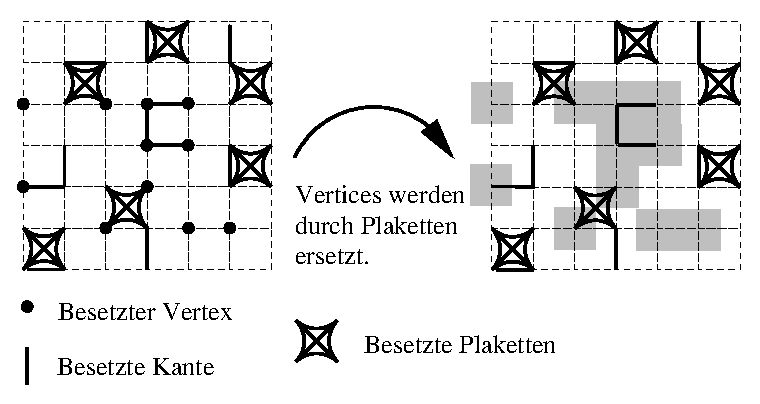
\includegraphics{./Mixed-figs/mixed}
  \caption{Links ist eine m\"ogliche Konfiguration eines gemischten Perkolationsprozesses auf dem Quadratgitter dargestellt. Die Konfiguration enth\"alt auch isolierte Kanten, die keine Cluster bilden. Im ersten Schritt werden auf besetzte Vertices offene duale Quadrate gesetzt (rechts). Damit aus diesen Quadraten Figuren entstehen, die den Gitterclustern entsprechen, m\"ussen sie an den Kanten und Ecken in geeigneter Weise zusammengef\"ugt werden. }
  \label{fig:mixed}
\end{figure}
Die Konfiguration des urspr\"unglichen Gitters beschreiben wir, indem wir jedem Vertex $v$, jeder Kante $k$ und jeder Plakette $f$ eine Variable $\sigma(v)$, $\sigma(k)$ bzw. $\sigma(f)$ zuweisen, die jeweils die Werte $0$ und $1$ annehmen kann. Ist $\sigma=1$, ist der entsprechende Teil des Gitters besetzt. Um die Figuren auf dem dualen Gitter zu beschreiben, f\"uhren wir zu jeder dualen Plakette, jeder dualen Kante und jedem dualen Vertex eine weitere Variable $\lambda(c)$ ein, wobei $c$ die entsprechende Zelle des urspr\"unglichen Gitters bezeichnet.
\\Wir geben die $\sigma$'s auf dem urspr\"unglichen Gitter vor, und konstruieren aus den offenen dualen Zellen eine Figur, die den Gitterclustern entspricht. Jede Plakette des dualen Gitters geh\"ort zur Figur, wenn der Vertex $v$ des urspr\"unglichen Gitters besetzt ist, d.h. $\lambda(v)=\sigma(v)$. Dieser Schritt ist in Abb. \ref{fig:mixed} f\"ur einen Ausschnitt des Quadratgitters illustriert. Die geometrische Figur $F$ besteht nach diesem Schritt aus allen offenen Plaketten mit $\lambda(v)=1$. $F$ wird in den folgenden Schritten an Kanten und Ecken modifiziert, damit die Figur am Ende abgeschlossen ist, und ihre Komponenten den Gitterclustern entsprechen.
\paragraph{Kanten:} Wir betrachten nun eine Kante $k$. Im Fall $\sigma(k)=1$, wird die duale Kante von $k$ zu $F$ hinzuf\"ugt, vorausgesetzt mindestens eine der angrenzenden Plaketten ist besetzt. Wenn $\sigma(k)=0$ ist, und keine der benachbarten dualen Plaketten ist besetzt, wird die duale Kante von $k$ in $F$ nicht ben\"otigt. Ist nur eine der beiden angrenzenden dualen Plaketten besetzt, wird $k$ als Randzelle dieser Plakette zu $F$ hinzugef\"ugt. 
\begin{figure}[tbp]
  \centering
  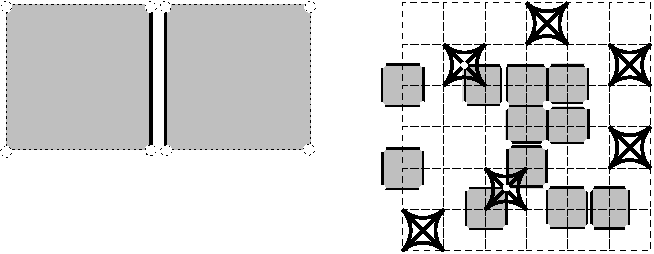
\includegraphics{./Mixed-figs/kanten2}
  \caption{Der zweite Schritt. Links: Zwei besetzte Plaketten, die etwas auseinanderger\"uckt sind, und mit je einer Kopie der Kante als Randst\"uck versehen werden.  Diese Kante hat $\lambda=2$. Alle anderen Randst\"ucke sind noch nicht vorhanden. Rechts ist die Figur aus Abb. \ref{fig:mixed} gezeigt, die um alle Kanten entsprechend der im Text beschrieben Prozedur erweitert wurde. Die Ecken der besetzten Plaketten fehlen noch.}
  \label{fig:kanten}
\end{figure}
Wenn beide angrenzenden dualen Plaketten besetzt sind, m\"ussen diese Plaketten infinitesimal auseinanderger\"uckt und je eine Kopie der dualen Kante von $k$ an beide Plaketten angef\"ugt werden (siehe Abb. \ref{fig:kanten}). Die duale Kante $\bar{k}$ ist dann zweimal in $F$ enthalten. Wir definieren $\lambda(k)$ als die Anzahl der in $F$ vorhandenen Kopien von $\bar{k}$. Seien $v_1(k)$ und $v_2(k)$ die Vertices des urspr\"unglichen Gitters, zwischen denen $k$ liegt. Dann ist 
\begin{equation}
\fbox{$\displaystyle
  \lambda(k):=\begin{cases} \lambda(v_1(k))+ \lambda(v_2(k)) \qquad & \text{falls}\;\; \sigma(k)=0, \\
 1-\left[1-\lambda(v_1(k))\right]\left[1-\lambda(v_2(k))\right] \qquad & \text{falls} \;\; \sigma(k)=1.\end{cases}
$}
\end{equation}
Wenn diese Prozedur an allen Kanten durchgef\"uhrt worden ist, besteht $F$ aus offenen Plaketten und Kanten ohne Randpunkte. Die Ecken der besetzten Plaketten fehlen noch. Die Figur $F$ der Konfiguration aus Abbildung \ref{fig:mixed} ist rechts in Abbildung \ref{fig:kanten} in diesem Zustand gezeigt.

\paragraph{Ecken:} Wenn eine Plakette $f$ des Gitters dekoriert ist, d.h. $\sigma(f)=1$ ist, sind alle Vertices auf dem Rand der Plakette miteinander verbunden. Die dualen Plaketten der Vertices auf dem Rand von $f$ \"uberlappen alle am dualen Vertex $\bar{f}$ von $f$. Wird $\bar{f}$ zu $F$ hinzugef\"ugt, werden daher die geforderten Zusammenhangsverh\"altnisse erzeugt. Sei nun $f$ eine Plakette mit $\sigma(f)=0$. Um die gew\"unschten Zusammenhangsverh\"altnisse zu erzeugen, entfernen wir aus $F$ eine kleine, um die duale Ecke $\bar{f}$ der Plakette $f$ zentrierte, offene Kreisscheibe $B_r(f)$ mit Radius $r$ (siehe links in Abb. \ref{fig:ecken}). Die neue Figur $F_r'(f)$ ist dann
\begin{equation}
  F_r'(f)=F\backslash B_r(f).
\end{equation}
Sei nun $S_r(f)$ ein Kreisring mit Mittelpunkt bei $\bar{f}$ und Radius $r$. Die neu entstandenen Randst\"ucke sind der Durchschnitt von $S_r(f)$ mit $F$ (siehe Abb. \ref{fig:ecken}). Den Durchschnitt bezeichnen wir mit $\Lambda_r(f):=S_r(f)\cap F$. 
\begin{figure}[tbp]
  \centering
  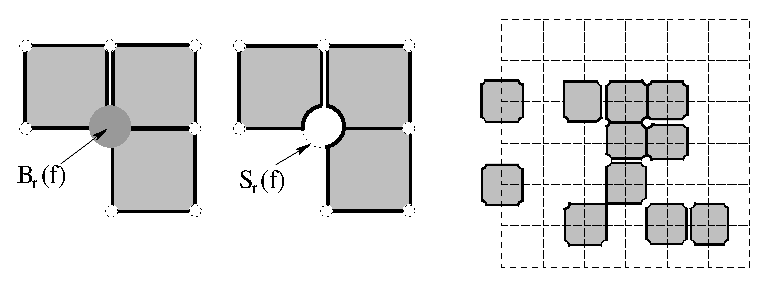
\includegraphics{./Mixed-figs/ecken}
  \caption{Der dritte Schritt: Damit die dualen Plaketten von Vertices auf dem Rand einer undekorierten Plakette $f$ des urspr\"unglichen Gitters nicht zusammenh\"angen, die Figur aber dennoch abgeschlossen ist, wird eine offene Kreisscheibe $B_r(f)$, zentriert an der dualen Ecke $\bar{f}$, entfernt. Die neu entstandenen Randst\"ucke sind der Durchschnitt $\Lambda_r(f)=S_r(f)\cap F$ des Kreises $S_r(f)$ mit $F$. $\Lambda_r(f)$ h\"angt nicht nur von den $\bar{f}$ umgebenden Plaketten ab, sondern auch davon, ob diese verbunden sind oder nicht. Die Euler-Charakteristik $\chi(\Lambda_r)$ ist im dargestellten Fall zwei. Rechts ist die Figur aus Abb. \ref{fig:mixed} dargestellt, nachdem sie an allen Kanten und Ecken modifiziert worden ist. }
  \label{fig:ecken}
\end{figure}
\\Im Limes $r \rightarrow 0$ werden die Beitr\"age der dualen Plaketten und Kanten zu Fl\"ache, Umfang und Euler-Charakteristik nicht ver\"andert. Die Randst\"ucke $\Lambda_r(f)$ tragen f\"ur $r\rightarrow 0$ nur zur skalenunabh\"angigen Euler-Charakteristik bei. Das neue, durch die Modifikation ver\"anderte, $F$ ist
\begin{equation}
  F=\lim_{r\rightarrow 0}F_r'(f),
\end{equation}
und der Beitrag einer Ecke zur Euler-Charakteristik von $F$ ist $\chi(\Lambda_r(f))$.
Seien nun $v_i(f)$ und $k_i(f)$ die Kanten und Plaketten, die die Ecke umgeben. F\"ur jede Ecke $f$ definieren wir  
\begin{equation}
  \lambda(f):= \begin{cases} \chi(\Lambda_r(f)) \qquad & \text{falls} \;\; \sigma(f)=0, \\ 1-\prod_{i=1}^n\left[1-\lambda(v_i(f))\right] \qquad & \text{falls} \;\; \sigma(f)=1.
\end{cases}
\end{equation}
$\Lambda_r(f)$ ist eine Vereinigung von Kreissegmenten. Jeder Schnitt des Kreises mit einer besetzten Plakette ist ein offenes Kreissegment. Der Schnitt des Kreises mit den $\lambda(k_i(f))$-fach vorhanden Kanten $k_i(f)$ sind Punkte, die den Abschluss der offenen Kreissegmente bilden. Daher ist  
 \begin{equation}
\fbox{$\displaystyle
  \lambda(f)= \begin{cases} \sum_{i=1}^n \lambda(k_i(f))-\sum_{i=1}^n\lambda(v_i(f)) \qquad & \text{falls} \;\; \sigma(f)=0, \\ 1-\prod_{i=1}^n\left[1-\lambda(v_i(f))\right] \qquad & \text{falls} \;\; \sigma(f)=1.
\end{cases}
$}
\end{equation}
Diese Prozedur muss f\"ur jede Plakette $f$ durchgef\"uhrt werden. Die Figur, die zur Gitterkonfiguration aus Abbildung \ref{fig:mixed} geh\"ort, ist rechts in Abbildung \ref{fig:ecken} dargestellt. \\
 
Sind alle Modifikationen und Erg\"anzungen durchgef\"uhrt, erh\"alt man f\"ur die Euler-Charakteristik der Figur $F$:
\begin{equation}
\fbox{$\displaystyle
  \chi(F)=\sum_{f}\lambda(f)-\sum_{k}\lambda(k)+\sum_{v}\lambda(v).
$}
\end{equation}
Entsprechend k\"onnen auch Umfang und Fl\"ache durch die Summe der Beitr\"age aller Zellen, jeweils multipliziert mit $\lambda$, ausgerechnet werden.
\\Ist $\sigma(f)$ einer Plakette $f$ gleich 0 und sind alle Vertices und Kanten auf dem Rand von $f$ besetzt, entsteht durch die Modifikation ein Loch. Soll dies vermieden werden, muss $\sigma(f)$ in diesem Fall gleich 1 gesetzt werden. 
\\Die Erwartungswerte der $\lambda$'s werden f\"ur unterschiedliche Perkolationskonfigurationen am Ende dieses Kapitels ausgerechnet. Alle bisher berechneten Euler-Charakteristiken lassen sich durch geeignete Wahl der $\sigma$'s erhalten. 

\section{Gemischte Perkolation in drei Dimensionen}
Ein dreidimensionales Gitter l\"asst sich, anders als die planares Gitter, im Allgemeinen nicht in Zellen zerlegen. Daher betrachten wir ohne Bezug auf ein Gitter eine Tessellation des dreidimensionalen Raumes. Eine Tessellation ist eine Anordnung von nicht \"uberlappenden Polyedern, so dass ihre Vereinigung den gesamten $\mathbb{R}^3$ bedeckt \cite{Weygaert:91}. Die Polyeder bestehen aus ihrem dreidimensionalen Inneren und 0- bis $2$-dimensionalen Randzellen. Mit $C_k$ bezeichnen wir die Menge der $k$-dimensionalen, randlosen Zellen. Die Polyeder werden besetzt, und besetzte Polyeder k\"onnen \"uber gemeinsame Randzellen miteinander verbunden sein. 
\\Wir weisen jedem $c_k\in C_k$, $k\in \{ 0,\ldots, 3\}$, eine Variable $\sigma(c_k)\in \{0,1\}$ zu. F\"ur ein Polyeder $c_3$ bedeutet $\sigma(c_3)=1$, dass $c_3$ besetzt ist. F\"ur $c_k$, $k<3$, bedeutet $\sigma(c_k)=1 $, dass alle Polyeder, deren Rand die Zelle $c_k$ enth\"alt, \"uber $c_k$ verbunden sind. Wenn $\sigma(c_k)=0$ ist sollen diese Polyeder nicht \"uber $c_k$ verbunden sein. Die $\sigma$-Variablen erf\"ullen also die gleiche Funktion wie im zweidimensionalen Fall aus Kapitel \ref{sec:2dmixed}, werden aber anstatt mit Bestandteilen des Gitters, mit Zellen der Tesselation indiziert.
\\Wir konstruieren nun zu einem gegebenen Satz von $\sigma$'s ein geometrisches Objekt, das die geforderten Zusammenhangsverh\"altnisse hat. Zu jeder Zelle $c_k$ wird eine weitere Variable $\lambda(c_k)$ eingef\"uhrt, die die Beitr\"age der Zelle zur Figur beschreibt. Als Resultat erhalten wir die Minkowski-Funktionale $W_\nu(F)$ der so gewonnen Figur $F$. Die Minkowski-Funktionale sind ein vollst\"andiger Satz stetiger, additiver, geometrischer Gr\"o"sen \mbox{(siehe \cite{Mecke:94}).} In drei Dimensionen entsprechen ihnen das Volumen, die Oberfl\"ache, die integrale mittlere Kr\"ummung und die Euler-Charakteristik. Wie sich herausstellen wird, sind die $W_\nu(F)$ die Summe der $W_\nu(c_k)$ der einzelnen Zellen $c_k$, jeweils multipliziert mit einer ganzen Zahl $\lambda(c_k)$. Der Multiplikator $\lambda(c_k)$ l\"asst sich f\"ur $k<3$ immer aus den $\lambda$'s der $c_k$ umgebenden, h\"oherdimensionalen Zellen berechnen. 
\paragraph{Polyeder:}Alle besetzten Polyeder geh\"oren zur Figur $F$. F\"ur alle $c_3\in C_3$ ist $\lambda(c_3)=\sigma(c_3)$, und $F$ besteht anfangs nur aus diesen offenen Polyedern. F\"ur diese offenen Zellen wird, bei den Fl\"achen beginnend, ein Rand konstruiert, so dass die resultierende Figur $F$ die durch die $\sigma$'s vorgegebenen Zusammenhangsverh\"altnisse hat. 
\paragraph{Fl\"achen:}
Wenn f\"ur eine Fl\"ache $c_2$ $\sigma(c_2)=1$ ist, und mindestens einer der beiden Polyeder $c_3^1(c_2)$ und $c_3^2(c_2)$, die $c_2$ als gemeinsame Randfl\"ache haben, besetzt ist, wird $c_2$ zu $F$ hinzugef\"ugt. Im Fall $\sigma(c_2)=0$ wird an die Polyeder, sofern sie besetzt sind, je eine Kopie der Fl\"ache angef\"ugt. Wenn beide Polyeder besetzt sind, muss der Spalt zwischen ihnen infinitesimal ``verbreitert'' werden. Analog zu den Kanten im zweidimensionalen Fall gilt f\"ur die $\lambda(c_2)$ einer Fl\"ache $c_2$
\begin{equation}
\fbox{$\displaystyle  \lambda(c_2):=\begin{cases} \lambda(c_3^1(c_2))+ \lambda(c_3^2(c_2)) \qquad & \text{falls}\;\; \sigma(c_2)=0, \\
 1-\left[1-\lambda(c_3^1(c_2))\right]\left[1-\lambda(c_3^2(c_2))\right] \qquad & \text{falls} \;\; \sigma(c_2)=1.\end{cases}$}
\end{equation}
Diese Prozedur wird an allen Fl\"achen durchgef\"uhrt.
\paragraph{Kanten:} Eine Kante $c_1$ wird zu $F$ hinzugef\"ugt, wenn $\sigma(c_1)=1$ ist und mindestens einer der Polyeder $c_3^i(c_1)$, $i=1,\ldots,n$, in deren Rand $c_1$ ist, besetzt ist. Gegebenenfalls muss die Umgebung der Kante derart deformiert werden, dass das Hinzuf\"ugen der Kante alle umliegenden Polyeder und Fl\"achen verbindet (siehe Abb. \ref{fig:kante3d}). Im Fall $\sigma(c_1)=0$ muss $F$ entlang $c_1$ modifiziert werden, denn $c_1$ darf die Polyeder $c_3^i(c_1)$ nicht verbinden. $F$ muss aber entlang $c_1$ abgeschlossen sein. Dazu betrachten wir die offene Kreisscheibe $B_r(c_1)$ mit Radius $r$, die senkrecht auf $c_1$ steht. Der Mittelpunkt von $B_r(c_1)$ sei am Ursprung. Die Minkowskisumme der randlosen Zelle $c_1$ mit $B_r(c_1)$ wird aus $F$ entfernt. Die Minkowskisumme $B_r(c_1)\uplus c_1$ ist die Menge, die entsteht, wenn der Mittelpunkt von $B_r(c_1)$ an jeden Punkt von $c_1$ angeheftet wird (siehe Abb. \ref{fig:minkowski} und \cite{Mecke:94}). 
\begin{figure}[bt]
  \centering
  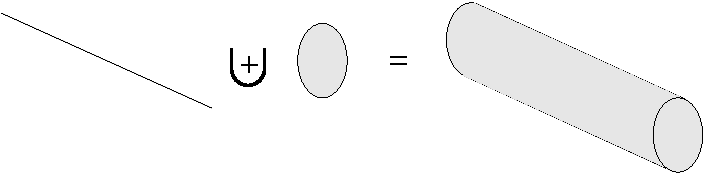
\includegraphics{./Mixed-figs/minkowski}
  \caption{Minkowskisumme einer Kante mit einer Kreisscheibe.}
  \label{fig:minkowski}
\end{figure}
\begin{figure}[bt]
  \centering
  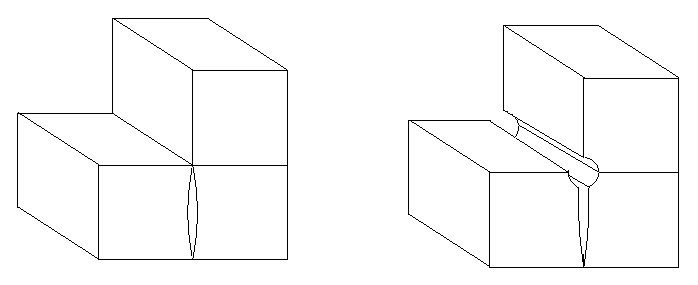
\includegraphics{./Mixed-figs/kante3d}
  \caption{Links sind drei W\"urfel dargestellt, deren gemeinsame Kante $c_1$ $\sigma(c_1)=1$ hat. Die beiden unteren W\"urfel sind nicht \"uber eine Fl\"ache verbunden, aber an der Kante $c_1$. Rechts sind die gleichen W\"urfel mit $\sigma(c_1)=0$ gezeigt. Der Durchschnitt eines hinreichend kleinen Kreises, angeheftet an die Kante, mit der Umgebung, ist in jedem Punkt der Kante gleich. Nur an den Randbereichen der Kante gilt das i. A. nicht. Diese Bereiche verschwinden aber mit dem Radius des Kreises. }
  \label{fig:kante3d}
\end{figure}
Die Menge $F'_r(c_k):=F\backslash(B_r(c_k)\uplus c_k)$ ist entlang $c_1$ abgeschlossen, und die umliegenden Polyeder h\"angen nicht \"uber $c_1$ zusammen (siehe Abb. \ref{fig:kante3d}).  
\\Um $W_\nu(F'_r(c_k))$ zu berechnen, betrachten wir den Kreisring $S_r(c_1)$. Die Vereinigung von $S_r(c_1)$ mit der offenen Kreisscheibe $B_r(c_1)$ ist die abgeschlossene Kreisscheibe $\bar{B}_r(c_1)$.  Mit $S_r(c_1)$ und $\bar{B}_r(c_1)$ l\"asst sich $F'_r(c_1)$ als disjunkte Vereinigung der modifizierten Figur $F$ mit den neuen Randst\"ucken schreiben: 
\begin{equation}
  F'_r(c_1)=\left( F\backslash (\bar{B}_r(c_1) \uplus c_1)\right) \cup \left( F\cap (S_r(c_1)\uplus c_1)\right).
\end{equation}
Wegen der Additivit\"at der Minkowski-Funktionale gilt  
\begin{equation}
\label{eq:modifikation}
  W_\nu(F'_r(c_1))=W_\nu\left(F\backslash(\bar{B}_r(c_1)\uplus c_1)\right)+W_\nu\left(F\cap (S_r(c_1) \uplus c_1)\right).
\end{equation}
Wegen der Stetigkeit der Minkowski-Funktionale gilt im Limes $r \rightarrow 0$ f\"ur den ersten Term auf der rechten Seite von Gleichung (\ref{eq:modifikation}) $W_\nu(F\backslash(\bar{B}_r(c_1)\uplus c_1))\rightarrow W_\nu(F\backslash c_1)=W_\nu(F)$. Die Beitr\"age der Polyeder und Fl\"achen werden durch die Modifikation im Limes $r\rightarrow 0$ also nicht ver\"andert, und alle zus\"atzlichen Beitr\"age kommen von den neuentstandenen Randst\"ucken entlang $c_1$. 
\\Im Limes $r\rightarrow 0$ ist $F\cap (S_r(c_1)\uplus x)$ mit $x\in c_1$ f\"ur alle $x$ gleich (abgesehen von einer Translation, siehe Abb. \ref{fig:kante3d}), und es gibt ein $\Lambda_r(c_1)$, so dass $F\cap (S_r(c_1)\uplus c_1)=\Lambda_r(c_1)\uplus c_1$ gilt. $\Lambda_r(c_1)$ ist die an den Ursprung verschobene Menge $F\cap (S_r(c_1)\uplus x)$.
Da $\Lambda_r(c_1)$ und $c_1$ in komplement\"aren, orthogonalen Unterr\"aumen liegen, ist die Formel $51$, Kapitel $6$ aus \cite{Hadwinger:57} anwendbar, und man erh\"alt f\"ur den zweiten Term in Gleichung (\ref{eq:modifikation})
\begin{equation}
  \label{eq:hadwinger}
  W_{\nu}(c_1\uplus\Lambda_r(c_1))=\frac{\omega_{\nu}}{{d \choose \nu}}\sum_{\mu=0}^{\nu}{k\choose \mu}{d-k \choose \nu-\mu}\frac{W'_{\mu}(c_1)W'_{\nu-\mu}(\Lambda_r(c_1))}{\omega_{\mu}\omega_{\nu-\mu}}.
\end{equation}
Im Limes $r \rightarrow 0$ verschwinden alle skalenabh\"angigen  $W'_{\nu-\mu}(\Lambda_r(c_1))$ und obige Formel vereinfacht sich zu 
\begin{equation}
 \lim_{r \rightarrow 0} W_{\nu}(c_1\uplus\Lambda_r(c_1))=W_{\nu}(c_1)\chi(\Lambda(c_1)).
\end{equation}
Damit wird aus Gleichung (\ref{eq:modifikation}) im Limes $r \rightarrow 0$
\begin{equation}
 \lim_{r\rightarrow 0} W_\nu(F'_r(c_1))=W_\nu\left(F\right)+W_\nu(c_1)\chi(\Lambda(c_1)).
\end{equation}
Die Euler-Charakteristik $\chi(\Lambda_r(c_1))$ ist unabh\"angig vom Radius $r$, der daher weggelassen wird. Die Beitr\"age der Modifikation zu den Minkowski-Funktionalen sind also die Minkowski-Funktionale der Zelle $c_1$, multipliziert mit der ganzen Zahl $\chi(\Lambda(c_1))$. Die Multiplizit\"at der Kante $c_1$ wird durch 
\begin{equation}
\fbox{$ \displaystyle 
  \lambda(c_1):= \begin{cases} \chi(\Lambda(c_1)) \qquad & \text{falls} \;\; \sigma(c_1)=0, \\ 1-\prod_{i=1}^n\left[1-\lambda(c_3^i(c_1))\right] \qquad & \text{falls} \;\; \sigma(c_1)=1,
\end{cases}
$}
\end{equation}
definiert. $\Lambda(c_1)$ ist der Durchschnitt eines Kreisrings mit den besetzten Polyedern $c_3^i(c_1)$ und den zwischen ihnen liegenden $\lambda(c_2^1(c_1))$-fach vorhandenen Fl\"achen $c_2^i(c_1)$. $\Lambda(c_1)$ liegt in einer Ebene senkrecht auf $c_1$, und die entstehenden Schnittmuster sind Kreissegmente, analog zu dem Schnitt eines Kreises mit den dualen Plaketten und Kanten, die eine duale Ecke des zweidimensionalen Gitters umgeben (siehe Abb. \ref{fig:ecken}). Jeder Schnitt mit einem besetzten Polyeder ist ein offenes Kreissegment, und die Schnitte mit den Fl\"achen liefern je $\lambda(c_2^i(c_1))$ Punkte. Die Euler-Charakteristik von $\Lambda(c_1)$ ist daher
 \begin{equation}
 \chi(\Lambda(c_1))= \sum_{i=1}^n \lambda(c_2^i(c_1))-\sum_{i=1}^n\lambda(c_3^i(c_1)).
\end{equation}   
Die Figur $F$ wird jetzt durch $\lim_{r\rightarrow 0}F'_r(c_k)$ ersetzt, und die Prozedur nacheinander an allen Kanten durchgef\"uhrt. 
\paragraph{Ecken:} Eine Ecke $c_0$ der Tesselation wird von Polyedern $c_3^1(c_0),\ldots,c_3^n(c_0)$, Fl\"achen $c_2^1(c_0),$ \ldots,$c_2^m(c_0)$ und Kanten $c_1^1(c_0),\ldots,c_1^l(c_0)$ umgeben. Ist $\sigma(c_0)=1$ und mindestens einer der umgebenden Polyeder besetzt, wird $c_0$ zu $F$ hinzugef\"ugt und verbindet die offenen Enden an der Ecke. Dazu ist gegebenfalls eine Deformation der Umgebung der Ecke n\"otig. Falls $\sigma(c_0)=0$ ist, wird eine offene Kugel $B_r(c_0)$ mit Radius $r$, zentriert bei $c_0$, aus $F$ entfernt. Wie im Fall einer Kante werden die Beitr\"age der h\"oherdimensionalen umgebenden Zellen zu den Minkowskifunktionalen im Limes $r\rightarrow 0$ nicht ver\"andert. Die neuen Randst\"ucke sind der Schnitt einer Sph\"are $S_r(c_0)$ mit $F$. Die Randst\"ucke $\Lambda_r(c_0)=S_r(c_0)\cap F$ tragen im Limes $r\rightarrow 0$ nur zur Euler-Charakteristik bei, und wir definieren $\lambda(c_0)$ durch $\chi(\Lambda_r(c_0))$. $\Lambda_r(c_0)$ besteht aus dem Schnitt von $S_r(c_0)$ mit den umgebenden besetzten Polyedern, den dazwischenliegenden $\lambda(c_2^i(c_0))$-fach vorhandenen Fl\"achen und den, gegebenenfalls modifizierten, Kanten. Jeder Schnitt mit einem besetzten Polyeder ist ein offenes Gebiet auf der Sph\"are und liefert den Beitrag $+1$. Der Schnitt mit einer $\lambda(c_2^i(c_0))$-fach vorhandenen Fl\"ache sind $\lambda(c_2^i(c_0))$ offene Geradenst\"ucke, die $-\lambda(c_2^i(c_0))$ zur Euler-Charakteristik beitragen. Der Schnitt der Sph\"are mit einer Kante ist ein Punkt und tr\"agt $+1$ bei. Die Umgebung von Kanten mit $\sigma(c_1^i(c_0))=0$ wurde aber modifiziert, und der Schnitt mit den durch die Modifikation entstandenen Randst\"ucken ist gerade $\lim_{r\rightarrow 0}\Lambda_r(c_1^i(c_0))$. Die Kanten tragen also $\lambda(c_1^i(c_0))$ zu Euler-Charakteristik bei. Damit ergibt sich: 
\begin{equation}
\label{eq:lambdaecken}
\fbox{$ \displaystyle 
  \lambda(c_0):= \begin{cases} \sum_{i=1}^n \lambda(c_3^i(c_0))-\sum_{i=1}^m\lambda(c_2^i(c_0))+\sum_{i=1}^l\lambda(c_1^i(c_0))\qquad & \text{falls} \;\; \sigma(c_0)=0, \\ 1-\prod_{i=1}^n\left[1-\lambda(c_3^i(c_0))\right] \qquad & \text{falls} \;\; \sigma(c_0)=1.
\end{cases}
$}
\end{equation}
Nachdem $F$ an allen Ecken auf diese Weise modifiziert wurde, ist $F$ abgeschlossen und hat die geforderten Zusammenhangsverh\"altnisse.
\\Die Minkowski-Funktionale von $F$ sind dann die Summe der Beitr\"age der einzelnen Zellen $c$, jeweils multipliziert mit der ganzen Zahl $\lambda(c)$:
\begin{equation}
\fbox{$\displaystyle
  W_{\nu}(F,\{\mathbf{\sigma}\})=\sum_{c}\lambda(c)W_{\nu}(c)
$}
\end{equation}

Wenn $\sigma(c_k)$ einer $k$-Zelle $c_k$ gleich null ist und alle umliegenden h\"oherdimensionalen Zellen $\sigma=1$ haben, wird durch die Modifikation ein $k$-dimensionaler Tunnel erzeugt. Wenn solche Tunnel vermieden werden sollen, muss $\sigma(c_k)$ in diesem Fall auf den Wert 1 gesetzt werden. 
\\

Die formale Behandlung der Modifikation an den Kanten l\"asst sich ohne weiteres auf die Fl\"achen und Ecken \"ubertragen. In entsprechender Weise kann der Formalismus auch auf $d$-dimensionale Tesselationen verallgemeinert werden. Da dies in dieser Arbeit nicht ben\"otigt wird, beschr\"anken wir uns auf zwei und drei Dimensionen.  

\section{Anwendung auf Perkolationskonfigurationen}

\subsection{bond-site Perkolation}
\label{sec:bond-site}
Bei bond-site-Perkolation werden Vertices eines Gitters mit Wahrscheinlichkeit $p_s$ und Kanten des Gitters mit Wahrscheinlichkeit $p_b$ besetzt. Wir wenden nun den oben erarbeiteten Formalismus auf bond-site-Perkolation in drei Dimensionen an und betrachten dazu ein Gitter, zu dem Zellen existieren, deren Fl\"achen den Gitterkanten entsprechen. Diese Zellen bilden die Tesselation aus dem vorhergehenden Abschnitt.
\\Jede dreidimensionale Zelle $c_3$ wird mit Wahrscheinlichkeit $p_s$ besetzt, d.h. mit Wahrscheinlichkeit $p_s$ ist $\sigma(c_3)=1$. Die Fl\"achen entsprechen den Gitterkanten und $\sigma$ jeder Fl\"ache wird mit Wahrscheinlichkeit $p_b$ auf den Wert 1 gesetzt. Die $\sigma$-Variablen der Kanten und Ecken haben den Wert 0, sofern nicht alle umliegenden $3$-Zellen und Fl\"achen $\sigma=1$ haben. Dadurch wird gew\"ahrleistet, dass entlang der Kanten und Ecken keine Tunnel bzw. Einschl\"usse entstehen, wenn alle umliegenden $3$-Zellen und Fl\"achen besetzt sind. Um die Erwartungswerte der $W_\nu$ zu berechnen, m\"ussen wir die Erwartungswerte $\left<\lambda(c)\right>_{p_s,p_b}$ aller Zellen kennen.
\\Der Erwartungswert $\left<\lambda_3\right>_{p_s,p_b}$ einer beliebigen $3$-Zelle ist $p_s$. Der Erwartungswert $\left<\lambda(c_2)\right>_{p_s,p_b}$ einer Fl\"ache $c_2$ setzt sich aus einem Beitrag mit $\sigma(c_2)=1$ und einem mit $\sigma(c_2)=0$ zusammen. Im ersten Fall ist $\lambda(c_2)=1$, wenn immer eine der angrenzenden $3$-Zellen besetzt ist; im zweiten Fall ist $\lambda(c_2)$ die Zahl der besetzten angrenzenden $3$-Zellen. F\"ur jede Fl\"ache $c_2$ gilt daher 
\begin{equation}
  \left<\lambda(c_2)\right>_{p_s,p_b}=\left<\lambda_2\right>_{p_s,p_b}=(1-(1-p_s)^2)p_b+2p_s(1-p_b)=2p_s-p_bp_s^2.
\end{equation}
Eine Kante $c_1$ umgeben die $3$-Zellen $c_3^1(c_1),\ldots,c_3^n(c_1)$ und die Fl\"achen $c_2^1(c_1),\ldots,c_2^n(c_1)$. Auch bei Kanten m\"ussen die F\"alle  $\sigma(c_1)=1$ und  $\sigma(c_1)=0$ unterschieden werden. Der erste Fall tritt mit der Wahrscheinlichkeit $p_s^np_b^n$ ein. Im zweiten Fall m\"ussen wir immer voraussetzen, dass nicht f\"ur alle $i\in \{1,\ldots,n\}$  $\sigma(c_3^i(c_1))=\sigma(c_2^i(c_1))=1$ gilt. Daher sind die Beitr\"age der einzelnen Fl\"achen und $3$-Zellen zu $\lambda(c_1)$ nicht mehr unabh\"angig und m\"ussen einzeln abgez\"ahlt werden. Zum Abz\"ahlen aller m\"oglichen Zust\"ande der umgebenden 3-Zellen und Fl\"achen und zur Berechnung der $\lambda(c_1)$ habe ich ein Computerprogramm (siehe dazu Anhang \ref{sec:noofcomp}) geschrieben.  
\\Eine Ecke $c_0$ sei von den $3$-Zellen $c_3^1(c_0),\ldots,c_3^m(c_0)$, den Fl\"achen $c_2^1(c_0),\ldots,c_2^n(c_0)$ und den Kanten $c_1^1(c_0),\ldots,c_1^l(c_0)$ umgeben. Wenn $\sigma(c_3^i(c_0))=1$ f\"ur alle $i\in \{1,\ldots,m\}$ und $\sigma(c_2^i(c_0))=1$ f\"ur alle $i\in \{1,\ldots,n\}$ gilt, ist $\sigma(c_0)=1$. Anderfalls, muss $\chi(\Lambda(c_0))$ berechnet werden. Hierzu werden wieder alle m\"oglichen Zust\"ande der umgebenden Zellen und Fl\"achen abgez\"ahlt und jeweils $\lambda(c_0)$ berechnet.
\\Da die Berechnung der $\left<\lambda_3\right>_{p_s,p_b}$, $\left<\lambda_2\right>_{p_s,p_b}$ und $\left<\lambda_1\right>_{p_s,p_b}$ in drei Dimensionen der Berechnung der $\left<\lambda_2\right>_{p_s,p_b}$, $\left<\lambda_1\right>_{p_s,p_b}$ bzw. $\left<\lambda_0\right>_{p_s,p_b}$ in zwei Dimensionen entspricht, kann bond-site-Perkolation auf zweidimensionalen Gittern v\"ollig analog behandelt werden. 


\subsubsection{Euler-Charakteristik der bond-site-Perkolation auf dem Quadratgitter}
\label{sec:bondsitesq}
Um die Euler-Charakteristik der bond-site-Perkolation auf dem Quadratgitter zu erhalten, muss nur noch $\left<\lambda(c_0)\right>_{p_s,p_b}$ jeder dualen Ecke $c_0$ bestimmt werden. Alle Ecken des Quadratgitters werden von vier Quadraten umgeben. Daher ist $\left<\lambda(c_0)\right>_{p_s,p_b}$ einer Ecke $c_0$ f\"ur alle Ecken gleich $\left<\lambda_0\right>_{p_s,p_b}$. 
Alle m\"oglichen Konfigurationen der vier Quadrate und Kanten werden abgez\"ahlt, und die $\lambda_0$ mit ihrer Wahrscheinlichkeit gewichtet und aufsummiert. Man erh\"alt 
\begin{equation}
    \left<\lambda_0\right>_{p_s,p_b} = 4p_s+p_b^4p_s^4-4p_bp_s^2.
\end{equation}
Die mittlere Euler-Charakteristik der bond-site-Perkolation auf dem Quadratgitter ist damit:
\begin{equation}
  \label{eq:bondsitesq}
  \fbox{$ \chi(p_s,p_b)=p_s-2p_bp_s^2+p_b^4p_s^4.$}
\end{equation}
\subsubsection{Euler-Charakteristik der bond-site-Perkolation auf dem einfach kubischen Gitter}
\label{sec:bondsitesc}
Die Zellen des einfach kubischen Gitters (sc-Gitter) sind W\"urfel. Da jede Kante von vier W\"urfeln umgeben ist, gilt f\"ur das sc-Gitter, analog zum zweidimensionalen Quadratgitter,
\begin{eqnarray} 
  \left<\lambda_3\right>_{p_s,p_b} &=& p_s,\\
  \left<\lambda_2\right>_{p_s,p_b} &=& 2p_s-p_bp_s^2,\\
  \left<\lambda_1\right>_{p_s,p_b} &=& 4p_s+p_b^4p_s^4-4p_bp_s^2.
\end{eqnarray}
Eine W\"urfelecke ist von acht W\"urfeln, zw\"olf Fl\"achen und sechs Kanten umgeben. Zu jeder m\"oglichen Konfiguration muss $\lambda_0$ aus den $\lambda$'s aller W\"urfel, Fl\"achen und Kanten bestimmt werden. 
Die Summation aller Beitr\"age liefert 
\begin{equation}
\left<\lambda_0\right>_{p_s,p_b}=8p_s-12p_bp_s^2+6p_b^4p_s^4-p_b^{12}p_s^8.
\end{equation}
Pro W\"urfel gibt es je drei Fl\"achen und Kanten, sowie eine Ecke, und f\"ur die Euler-Charakter\-istik (siehe Abb.  \ref{fig:chi-bond-site}) erh\"alt man  
\begin{equation}
  \label{eq:bondsitesc}
\fbox{$
\begin{split}
\chi(p_s,p_b)&=  \left<\lambda_0\right>_{p_s,p_b}-3\left<\lambda_1\right>_{p_s,p_b}+3\left<\lambda_2\right>_{p_s,p_b}-\left<\lambda_3\right>_{p_s,p_b}\\
&= p_s-3p_s^2p_b+3p_s^4p_b^4-p_s^8p_b^{12}.
\end{split}$}
\end{equation}\\

Die mittleren Euler-Charakteristiken des Quadrat- (Gl. \ref{eq:bondsitesq}) und des sc-Gitters (Gl. \ref{eq:bondsitesc}) sind f\"ur $p_s=0$ konstant null, da ein Cluster mindestens einen besetzten Vertex enthalten muss, und daher f\"ur $p_s=0$ keine Cluster existieren (siehe Abb. \ref{fig:chi-bond-site}). 
\begin{figure}[bt]
  \centering
  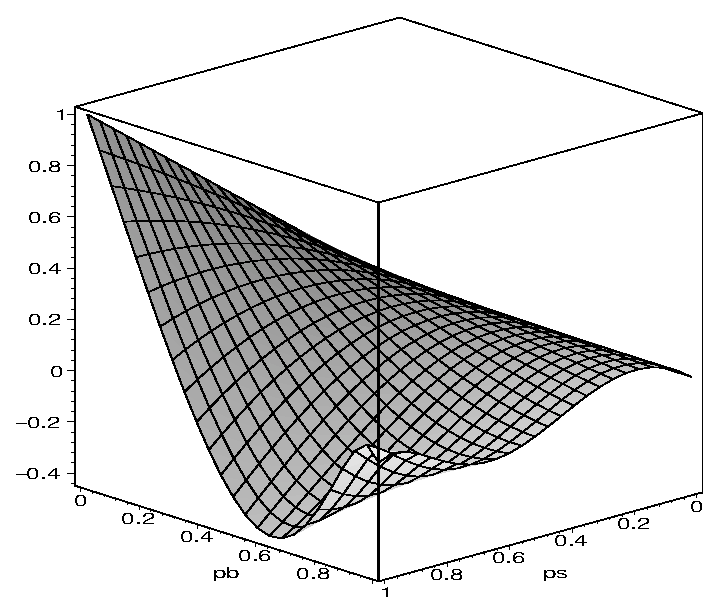
\includegraphics{./Mixed-figs/chibondsiteplot}
  \caption{Euler-Charakteristik $\chi(p_s,p_b)$ der bond-site-Perkolation auf dem sc-Gitter.}
  \label{fig:chi-bond-site}
\end{figure}
F\"ur $p_b=0$ besteht die Anordnung aus isolierten abgeschlossenen Zellen und $\chi(p_s,0)=p_s$. Der Fall $p_b=1$ wird die Euler-Charakteristik der site-Perkolation auf dem Quadrat- bzw. sc-Gitter reproduziert. F\"ur $p_s=1$ ist $\chi(p_s=1,p_b)$ die Euler-Charakteristik des reinen bond-Perkolationsprozesses des Quadrat- bzw. sc-Gitters. 

\subsection{Euler-Charakteristik des bcc-Gitters}
\label{sec:mixedbcc}
Neben der Berechnung der Euler-Charakteristik von bond-site-Perkolationsprozessen eignet sich der vorgestellte Formalismus auch, um bei reinen site-Perkolationsproblemen bestimmte Nachbarschaftsverh\"altnisse zu erzwingen, wenn keine geeigneten Zellen mit den Nachbarschaftsverh\"altnissen des Gitters gefunden werden k\"onnen. Am Beispiel der Wigner-Seitz-Zelle (WSZ) des bcc-Gitter soll eine solche Anwendung hier vorgef\"uhrt werden. Die WSZ des bcc-Gitters hat 14 Fl\"achen, ein Gittervertex aber nur acht n\"achste Nachbarn. Um eine mittlere Euler-Charakteristik zu erhalten, die der 8-Nachbarschaft entspricht, k\"onnen entweder komplizierte nicht konvexe Zellen (siehe Abb. \ref{fig:bcc_nonconvex_app}) gew\"ahlt werden, oder auf den Fl\"achen der WSZ die $\sigma$'s entsprechend der 8-Nachbarschaft vorgegeben werden (siehe Abb. \ref{fig:bccconvexapp}). Die sechseckigen Fl\"achen entsprechen Gitternachbarschaften und haben $\sigma=1$. Die Quadrate entsprechen keinen Gitternachbarschaften und haben $\sigma=0$, falls die beiden angrenzenden Zellen keinen gemeinsamen besetzten Gitternachbarn haben. Andernfalls ist $\sigma=1$. 
\begin{figure}[htbp]
  \centering
  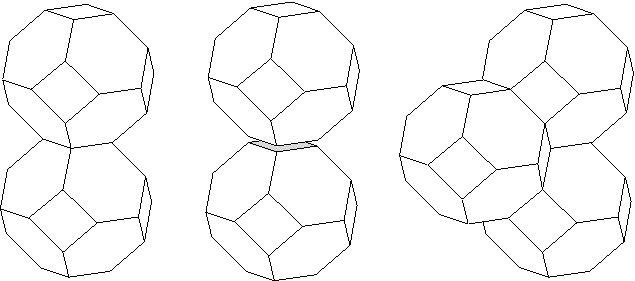
\includegraphics{./Mixed-figs/bcc_nn}
  \caption{WSZ des bcc-Gitter gelten nur als benachbart, wenn sie n\"achste Nachbarn sind (sechseckige Fl\"achen) oder einen gemeinsamen n\"achsten Nachbar haben: Zwei WSZ die sich an einem Quadrat ber\"uhren (links), werden getrennt (Mitte), solange sie keinen gemeinsamen n\"achsten Nachbar haben (rechts).}
  \label{fig:bccconvexapp}
\end{figure}
WSZ werden mit Wahrscheinlichkeit $p=1-q$ besetzt, und $\left<\lambda_3\right>_{p}=p$. F\"ur Sechsecke gilt $\left<\lambda_2^{hex}\right>_{p}=1-q^2=2p-p^2$. F\"ur ein Quadrat ist $\lambda_2^{sq}=1$, wenn genau eine der beiden angrenzenden WSZ besetzt ist. Wenn beide besetzt sind, ist $\lambda_2^{sq}=1$, wenn mindestens einer der vier gemeinsamen Nachbarn besetzt ist, und anderfalls $\lambda_2^{sq}=2$. F\"ur den Erwartungswert erh\"alt man
\begin{equation}
 \left<\lambda_2^{sq}\right>_{p}=2pq+p^2(1-q^4)+2p^2q^4=2pq+p^2(1+q^4).
\end{equation}
Jede Kante $c_1$ ist im Rand eines Quadrates und zweier Sechsecke enthalten. Sobald mindestens eine der umliegenden Zellen besetzt ist, ist die Kante vorhanden. Nur wenn das Quadrat $\lambda=2$ hat, ist $\lambda(c_1)=2$ und man erh\"alt
\begin{equation}
 \left<\lambda_1\right>_{p}=(1-q^3)+p^2q^4. 
\end{equation}
Eine Ecke $c_0$ geh\"ort zu vier Zellen, von denen zwei Paare keine Gitternachbarn sind. Die Ecke ist vorhanden, wenn mindestens eine der vier Zellen besetzt ist. $\lambda(c_0)=2$, wenn zwei WSZ besetzt sind, die keine n\"achsten Nachbarn sind, und gleichzeitig keine der vier gemeinsamen Gitternachbarn besetzt sind. Daher ist
\begin{equation}
 \left<\lambda_0\right>_{p}=(1-q^4)+2p^2q^4. 
\end{equation}
Es gibt pro Zelle acht Sechsecke und sechs Quadrate, die je zu zwei Zellen geh\"oren, 36 Kanten, die zu drei Zellen geh\"oren, und 24 Ecken, die zu vier Zellen geh\"oren. F\"ur die Euler-Charakteristik pro Zelle oder Gittervertex ergibt sich mit dieser Methode
\begin{equation}
  \chi^{bcc}_{8-14}(p)=p-4p^2+12p^4-12p^5+3p^6.
\end{equation}

\subsection{Weitere Anwendungsm\"oglichkeiten}
Der vorgestellte Formalismus l\"asst sich auf jeden beliebigen Satz von $\sigma$-Variablen anwenden, und somit ist es m\"oglich, geometrische Eigenschaften von Figuren zu berechnen, deren Konstituenten auf unterschiedlichste Weise zusammenh\"angen. Insbesondere ist es auch vorstellbar, wechselwirkende Modelle zu betracheten, und topologische Fluktuationen in Mikroemulsionen zu behandeln \cite{Jung:00}. Topologischen Fluktuationen k\"onnen sowohl Euler-Charakteristik, als auch integrale mittlere Kr\"ummung und Oberfl\"ache, ver\"andern, und Beitr\"age zu den thermodynamischen Potentialen der Mikroemulsion liefern \cite{Likos:95}. Dadurch wird sich das Phasendiagramm der Mikroemulsion ver\"andern und unter Umst\"anden zu neuen Phasen f\"uhren.

   %18.9.03

\chapter{Euler-Charakteristik und Perkolationsschwellen}
\label{sec:schranken}

Nachdem wir in den vorangehenden Kapiteln Methoden vorgestellt haben, mit denen die mittlere Euler-Charakteristik f\"ur Perkolationsprozesse auf Gittern berechnet werden kann, werden im Folgenden die Euler-Charakter\-ist\-iken einer Vielzahl zwei- und dreidimensionaler Gitter bestimmt. Die Resultate liefern weitere empirische Best\"atigung f\"ur die in der Einleitung vorgestellten Beobachtungen. Dar\"uberhinaus unterst\"utzen Skalenargumente die Vermutung, dass f\"ur zweidimensionale Gitter die Nullstelle $p_0$ der Euler-Charakteristik \"uber der Perkolationsschwelle $p_c$ liegt, falls $p_c>\frac{1}{2}$ ist, und dass $p_0<p_c$ ist, falls $p_c<\frac{1}{2}$ ist. Mit der in Kapitel \ref{sec:mixed} beschriebenen Methode kann die Euler-Charakteristik f\"ur bond-site-Perkolation berechnet werden, und die Beziehung zwischen der Nullstelle der Euler-Charakteristik und der Perkolationsschwelle auf bond-site-Perkolation erweitert werden.


\section{Euler-Charakteristiken in zwei Dimensionen}

Die Perkolationsschwelle $p_c$ archimedischer Gitter (siehe Abschnitt \ref{sec:archilattices}) ist kleiner als die Nullstelle $p_0$ und gr\"o"ser als der Wendepunkt $p_0^{(2)}$ der mittleren Euler-Charakteristik. Das arithmetische Mittel aus $p_0$ und $p_0^{(2)}$ liefert eine exzellente Approximation von $p_c$. Die Ergebnisse der Untersuchung weiterer zweidimensionaler Gitter best\"atigen dieses Verhalten; f\"ur $p_c<\frac{1}{2}$ kehren sich beide Ungleichungen um und man findet $p_0<p_c<p_0^{(2)}$. Allerdings gibt es auch Gitter, f\"ur die diese Ungleichungen nicht gelten. Auf diese Gitter wird im Kapitel \ref{sec:grenzen} genauer eingegangen.

\subsection{Laves-Gitter}
Laves-Gitter sind die dualen Gitter der archimedischen Gitter \cite{Gruenbaum:86}. Da archimedische Gitter nur einen Vertextyp haben, sind alle Plaketten der Laves-Gitter gleich. Die Kantenzahl der Plaketten ist die Koordinationszahl $z$ des archimedischen Gitters. Wie im Kapitel \ref{sec:chimittel} beschrieben, betrachten wir die unabh\"angige Besetzung der Plaketten der archimedischen Gitter mit Wahrscheinlichkeit $q=1-p$. Im Folgenden beziehen sich die Begriffe Plaketten, Ecken und Kanten auf die archimedischen Gitter mit Vertexkonfiguration $(n_1,\ldots,n_z)$ (siehe Kapitel \ref{sec:archilattices}). Die Euler-Charakteristik l\"asst sich am einfachsten \"uber die Beitr\"age disjunkter Zellen berechnen. Dazu bestimmen wir die erwartete Anzahl der offenen Plaketten, der randlosen Kanten und der Ecken, die bei Besetzung der Vertices mit abgeschlossenen Plaketten bedeckt werden.
\begin{itemize}
\item Die \textbf{Plaketten} sind mit Wahrscheinlichkeit $q$ bedeckt.
\item Jede \textbf{Ecke} ist von $z$ Plaketten umgeben; diese Plaketten haben $n_i$ Ecken, $i=1\ldots,z$. Daher besteht zwischen der Zahl der Ecken $E$ und der Zahl der Plaketten $F$ die Beziehung  $F=E \sum_{i=1}^z \frac{1}{n_i}$. Eine Ecke ist bedeckt, wenn mindestens eine der umgebenden Plaketten besetzt ist, und daher mit Wahrscheinlichkeit $1-(1-q)^z=1-p^z$ vorhanden. Die erwartete Anzahl der bedeckten Ecken pro Plakette ist $\frac{1-p^z}{\sum_{i=1}^z \frac{1}{n_i}}$.
\item Da jede \textbf{Kante} an zwei Ecken endet, und von jeder Ecke $z$ Kanten ausgehen, gilt f\"ur die Zahl der Kanten $K$ und Ecken $E$ die Relation $2K=zE$. Eine Kante ist bedeckt, wenn mindestens eine der angrenzenden Zellen besetzt ist, und daher mit Wahrscheinlichkeit $1-(1-q)^2=1-p^2$ vorhanden. F\"ur die erwartete Anzahl der bedeckten Kanten pro Plakette erh\"alt man $\frac{z(1-p^2)}{2\sum_{i=1}^z \frac{1}{n_i}}$.
\end{itemize}
Mit diesen Gr\"o"sen ist die mittlere Euler-Charakteristik pro Vertex 
\begin{equation}
    \bar{\chi}(q) = q- \frac{z}{2 \sum_{i=1}^z \frac{1}{n_i}}(1-p^2)+\frac{1}{\sum_{i=1}^z \frac{1}{n_i}}(1-p^z).
\end{equation}
Die Euler-Charakteristik ist von der Reihenfolge, in der die Polygone um die Vertices angeordnet sind, unabh\"angig. Dar\"uberhinaus gilt f\"ur einen planaren, zusammenh\"angenden Graphen nach dem Euler'schen Satz $F-E+V=1$. Daraus erh\"alt man
\begin{equation}
  F\left(1-\frac{z}{2 \sum_{i=1}^z \frac{1}{n_i}}+\frac{1}{\sum_{i=1}^z \frac{1}{n_i}}\right)=1
\end{equation}
und weiter unter Vernachl\"assigung von Termen $\sim 1/F$ die Beziehung $\sum_{i=1}^z \frac{1}{n_i}=\frac{z}{2}-1$. Die Euler-Charakteristiken der dualen archimedischen Gitter h\"angen also nur von der Koordinationszahl $z$ der archimedischen Gitter ab:
\begin{equation}
 \bar{\chi}(q) =q-\frac{z}{z-2}(1-p^2)+\frac{2}{z-2}(1-p^z).
\end{equation}
Die Euler-Charakteristik des Komplements ist  
\begin{equation}
\fbox{$ \displaystyle
   \chi(p) =-\bar{\chi}(q)=p(1-p)\left( 1-\frac{2}{z-2}\sum_{i=1}^{z-2}p^{i}\right).$
}
\end{equation}
Die site-Perkolationsschwellen der Laves-Gitter sind, wo sie nicht exakt oder als archimedische Gitter bekannt sind, von van der Marck \cite{Marck:03} numerisch bestimmt worden. Die Ergebnisse sind in Tabelle \ref{tab:laves} zusammengefasst. Einen Plot der Daten findet man in Abbildung \ref{fig:2dallplots}. F\"ur Laves-Gitter gilt wie f\"ur archimedische Gitter $p_0^{(2)}\leq p_c \leq p_0$. Die Korrelation von $p_0$ und $p_0^{(2)}$ mit $p_c$ ist aber nicht so bemerkenswert gut wie bei den archimedischen Gittern. Die Euler-Charakteristik der Laves-Gitter h\"angt nur von der Kantenzahl der Plaketten des Gitters ab; die Perkolationsschwellen der Gitter, deren Plaketten gleich viele Kanten haben, sind aber i. A. unterschiedlich.

\begin{table}[tb]
\centering
\begin{tabular}{|l|l||r|r|r||r|}
\hline
Duales (archimedisches) Gitter & $\frac{\chi(p)}{p(1-p)}$ & $p_0$ & $p_0^{(2)}$&$\frac{p_0+p_0^{(2)}}{2}$&$p_c$  \\ \hline
\hline

$3,12^2$ &$1-2p$&$1/2$ & $1/2$&$1/2$&$1/2$\\ \hline
 
$4,6,12$ &$1-2p$&$1/2$ & $1/2$&$1/2$&$1/2$\\ \hline

$4,8^2$&$1-2p$&$1/2$ & $1/2$&$1/2$&$1/2$\\ \hline

$6^3$, Sechseckgitter &$1-2p$&$1/2 $ & $1/2$&$1/2$&$1/2$\\ \hline

$3,6,3,6$, Kagom\'egitter&$1-p-p^2$&$0.6180$ & $0.5774$&$0.5977$&$0.5848(2)$ \\ \hline

$3,4,6,4$ &$1-p-p^2$&$0.6180$ & $0.5774$&$0.5977$&$0.5824(2)$ \\ \hline

$4^4$, Quadratgitter&$1-p-p^2$&$0.6180$ & $0.5774$&$0.5977$&$0.5927$ \\ \hline

$3^4,6$ &$1-\frac{2(p+p^2+p^3)}{3}$&$0.6914$ & $0.6300$&$0.6607$& $0.6396(2)$ \\ \hline

$3^2,4,3,4$ &$1-\frac{2(p+p^2+p^3)}{3}$&$0.6914$ & $0.6300$&$0.6607$&$0.6500(2)$  \\ \hline

$3^3,4^2$ &$1-\frac{2(p+p^2+p^3)}{3}$&$0.6914$& $0.6300$&$0.6607$&$0.6476(2)$  \\ \hline

$3^6$, Dreiecksgitter&$1-\frac{p+p^2+p^3+p^4}{2} $&$0.7413$ & $0.6687$&$0.7050$&$0.6970(2)$ \\ \hline

 \hline

\end{tabular}
\caption{Die mittleren Euler-Charakteristiken der Laves-Gitter: Die erste Spalte enth\"alt die Vertexkonfigurationen der dualen archimedischen Gitter. Die zweite Spalte enth\"alt die reduzierte Euler-Charakteristik $\frac{\chi(p)}{p(1-p)}$ der Laves Gitter. In den folgenden Spalten sind die Nullstellen $p_0$ und die Wendepunkte $p_0^{(2)}$ von $\chi(p)$, sowie $\frac{p_0+p_0^{(2)}}{2}$ angegeben. In der letzten Spalte stehen die site-Perkolationsschwellen $p_c$ der Laves-Gitter. Die ersten vier Gitter bestehen nur aus Dreiecken; daher ist $p_c=\frac{1}{2}$. Die \"ubrigen Perkolationsschwellen, abgesehen vom Quadratgitter, wurden in \cite{Marck:03} numerisch bestimmt. Die Perkolationsschwelle des Quadratgitters stammt aus \cite{Suding:99}.}
\label{tab:laves}
\end{table}

\subsection{2-uniforme Gitter}
\label{sec:2-uniform}
Es liegt nahe, als Verallgemeinerung der archimedischen Gitter mit einem Vertextyp, entsprechende Gitter mit zwei unterschiedlichen Vertextypen zu betrachten. 2-uniforme Gitter sind Gitter aus regelm\"a"sigen Polygonen gleicher Kantenl\"ange und zwei verschiedenen Vertextypen (siehe \cite{Gruenbaum:86}). Es gibt genau 20 verschiedene 2-uniforme Gitter (siehe Abbildungen im Abschnitt \ref{sec:numerik2-uniform}). Diese Gitter lassen sich, analog zu den archimedischen Gittern, durch ihre Vertextypen charakterisieren. Jeder Vertextyp $\nu$ wird durch die Folge $(n_1,\ldots,n_{z_\nu})_{\nu}$ der Kantenzahlen $n_i$ der Polygone, die den Vertex umgeben, beschrieben. Dar\"uberhinaus ist der Anteil $s_\nu$ eines Vertextyps an der Gesamtzahl der Vertices zur Unterscheidung der Gitter wichtig. Bis auf die Gitter 18 und 19 (siehe \ref{sec:numerik2-uniform}) sind so alle Gitter eindeutig bezeichnet. Die Euler-Charakteristik eines Gitters ist durch $(n_1,\ldots,n_{z_\nu})_{\nu}$ und $s_\nu$ vollst\"andig festgelegt.\\
Um die Euler-Charakteristik zu berechnen, bestimmen wir die Zahlen der bedeckten Kanten und Ecken des dualen Gitters, wenn duale Plaketten mit Wahrscheinlichkeit $q=1-p$ besetzt werden. 
\begin{itemize}
\item Jedem Vertex entspricht eine duale \textbf{Plakette}, die mit Wahrscheinlichkeit $q$ besetzt ist. 
\item Zu jeder Kante des 2-uniformen Gitters gibt es eine duale \textbf{Kante}. Die mittlere Koordinationszahl des 2-uniformen Gitters ist $\bar{z}=s_1z_1+s_2z_2$. Daher ist die Zahl der Kanten pro dualer Plakette $\frac{\bar{z}}{2}$.  Die Kanten sind mit Wahrscheinlichkeit $1-p^2$ bedeckt und die erwartete Anzahl bedeckter Kanten pro dualer Plakette ist $\frac{\bar{z}(1-p^2)}{2}$.
\item Zu einem Vertex des Typs $\nu$ des 2-uniformen Gitter ``geh\"ort'' $1/n_{i}(\nu)$ der ihn umgebenden Plaketten mit Kantenzahl $n_{i}(\nu)$, $i=1,\ldots,z_\nu$. Jeder dieser Plaketten entspricht eine \textbf{Ecke} des dualen Gitter, die mit Wahrscheinlichkeit $1-p^{n_{i}(\nu)}$ bedeckt ist. Um die erwartete Anzahl der Ecken pro dualer Plakette zu bestimmen, muss man \"uber beide Vertextypen und alle die Vertices umgebenden Plaketten summieren, und erh\"alt $\sum_{\nu=1,2}\sum_{i=1}^{z_\nu}\frac{s_\nu}{n_{i}(\nu)}(1-p^{n_{i}(\nu)})$.  
\end{itemize}
F\"ur die Euler-Charakteristik ergibt sich dann:
\begin{equation}
  \bar{\chi}(q)=q-\frac{\bar{z}}{2}(1-p^2)+\sum_{\nu=1,2}\sum_{i=1}^{z_\nu}\frac{s_\nu}{n_{i}(\nu)}(1-p^{n_{i}(\nu)}).
\end{equation}
Hiervon kann ein Faktor $p(1-p)$ abgespalten werden und man erh\"alt
\begin{equation}
  \label{eq:2-uniform}
 \fbox{$\displaystyle \chi(p)=-\bar{\chi}(1-p)=p(1-p)\left( 1-p\sum_{\nu=1,2}\sum_{i=1}^{z_\nu}\frac{s_\nu}{n_{i}(\nu)}\sum_{\mu=0}^{n_{i}(\nu)-3}p^\mu \right). $}
\end{equation}
Die Euler-Charakteristiken der 20 Gitter sind in Tabelle \ref{tab:2-uniformchi} angegeben.
\\Die Beschr\"ankung auf zwei Vertextypen ist unwesentlich, und die entsprechend verallgemeinerte Formel gilt f\"ur beliebige planare Gitter mit $k$ Vertextypen (siehe auch \cite{Wagner:02}). F\"ur einen Vertextyp k\"onnen so die Euler-Charakteristiken der archimedischen Gitter berechnet werden.
\\Ich habe die Perkolationsschwellen der 2-uniformen Gitter numerisch mit einer Genauigkeit von $2*10^{-4}$ bestimmt. Die verwendeten numerischen Methoden sind im Appendix \ref{sec:numerik} angegeben; Besonderheiten der Gitter und finite-size-scaling Plots sind in Abschnitt \ref{sec:numerik2-uniform} aufgef\"uhrt. Die Resultate sind zusammen mit den Nullstellen $p_0$ und Wendepunkten $p_0^{(2)}$ der Euler-Charakteristiken in Tabelle \ref{tab:2-uniform} aufgef\"uhrt. Ein Plot der Daten ist in Abbildung \ref{fig:2dallplots} zu finden.  F\"ur alle 2-uniformen Gitter gilt $p_0^{(2)}<p_c<p_0$. Dar\"uberhinaus f\"allt das arithmetische Mittel aus  $p_0$ und $p^{(2)}_0$ fast mit der Perkolationsschwelle zusammen. Gr\"o"sere Abweichungen der Perkolationsschwelle vom arithmetischen Mittel finden sich bei den Gittern 16, 20 und 6. Alle drei Gitter haben sehr hohe Perkolationsschwellen und eine ausgepr\"agte Substruktur. Diese Substrukturen k\"onnen zus\"atzliche L\"ocher enthalten, ohne die Konnektivit\"at zu beeinflussen. Dadurch wird die Nullstelle der Euler-Charakteristik relativ zur Perkolationsschwelle abgesenkt. Die Einfl\"usse von Substrukturen werden in Kapitel \ref{sec:grenzen} weiter diskutiert. 
\begin{table}[tbp]
\centering
\begin{tabular}{|r|l|l|}
\hline
 Nr. & Vertexkonfiguration &$\frac{\chi(p)}{p(1-p)}$ \\
\hline
\hline
1 &$\frac{1}{2}(3^6)+\frac{1}{2}(3^4,6)$&$\frac{p^4-5p^3}{12}+\frac{5p^2}{6}-\frac{5p}{2}+1$ \\ \hline
2&$\frac{1}{4}(3^6)+\frac{3}{2}(3^4,6)$&$\frac{p^4-5p^3}{8}+\frac{5p^2-11p}{4}+1$ \\ \hline
3&$\frac{1}{2}(3^6)+\frac{1}{2}(3^3,4^2)$&$\frac{p^2-9p}{4}+1$ \\ \hline
4&$\frac{1}{3}(3^6)+\frac{2}{3}(3^3,4^2)$&$\frac{p^2-7p}{3}+1$ \\ \hline
5&$\frac{1}{7}(3^6)+\frac{6}{7}(3^2,4,3,4)$&$\frac{3p^2-17p}{7}+1$ \\ \hline
6&$\frac{1}{7}(3^6)+\frac{6}{7}(3^2,4,12)$&$\frac{p^{10}-11p^9+55p^8-165p^7+330p^6}{14}-33(p^5-p^4)-\frac{165p^3+84p^2-38p}{7}+1$ \\ \hline
7&$\frac{1}{7}(3^6)+\frac{6}{7}(3^2,6)$&$\frac{2p^4-10p^3+20p^2-26p}{7}+1$ \\ \hline
8&$\frac{1}{2}(3^4,6)+\frac{1}{2}(3^2,6^2)$&$\frac{p^4-5p^3+10p^2-14p}{4}+1$ \\ \hline
9&$\frac{1}{3}(3^3,4^2)+\frac{2}{3}(3^2,4,3,4)$&$\frac{p^2-5p}{2}+1$ \\ \hline
10&$\frac{1}{2}(3^3,4^2)+\frac{1}{2}(3^2,4,3,4)$&$\frac{p^2-5p}{2}+1$ \\ \hline
11&$\frac{1}{2}(3^3,4^2)+\frac{1}{2}(3,4,6,4)$&$\frac{p^4-5p^3}{12}+\frac{4p^2}{3}-3p+1$ \\ \hline
12&$\frac{2}{3}(3^3,4^2)+\frac{1}{3}(4^4)$&$\frac{2p^2-8p}{3}+1$ \\ \hline
13& $\frac{1}{2}(3^3,4^2)+\frac{1}{2}(4^4)$&$\frac{3p^2-11p}{4}+1$ \\ \hline 
14&$\frac{1}{2}(3^2,4,3,4)+\frac{1}{2}(3,4,6,4)$&$\frac{p^4-5p^3}{12}+\frac{4p^2}{3}-3p+1$ \\ \hline
15&$\frac{2}{3}(3^2,6^2)+\frac{1}{3}(3,6,3,6)$&$\frac{p^4-5p^3+10p^2}{3}-4p+1$ \\ \hline
16&$\frac{1}{2}(3,4,3,12)+\frac{1}{2}(3,12^2)$&$\frac{p^{10}-11p^9+55p^8-165p^7}{12}+\frac{330p^6-231(p^5-p^4)-165p^3+83p^2-31p}{4}+1$ \\ \hline
17&$\frac{2}{3}(3,4^2,6)+\frac{1}{3}(3,4,6,4)$&$\frac{p^4-5p^3+13p^2-21p}{6}+1$ \\ \hline
18&$\frac{4}{5}(3,4^2,6)+\frac{1}{5}(3,6,3,6)$&$\frac{p^4-5p^3+12p^2-18p}{5}+1$ \\ \hline
19&$\frac{4}{5}(3,4^2,6)+\frac{1}{5}(3,6,3,6)$&$\frac{p^4-5p^3+12p^2-18p}{5}+1$ \\ \hline
20&$\frac{1}{3}(3,4,6,4)+\frac{2}{3}(4,6,12)$&$\frac{p^{10}-11p^9+55p^8}{18}+\frac{-55p^7+110p^6-154p^5+155p^4-115p^3+67p^2-35p}{6}+1$ \\ \hline

\hline
\end{tabular}
\caption{Die reduzierten mittleren Euler-Charakteristiken der 2-uniformen Gitter. Die Spalte ``Nr.'' enth\"alt die in \cite{Gruenbaum:86} angegebene Reihenfolge.}
\label{tab:2-uniformchi}
\end{table}
\begin{table}[tbp]
\centering
\begin{tabular}{|r|r|l|r|r|r||r|}
\hline
 Label & Nr. & Vertexkonfiguration & $p_0$ &  $p_0^{(2)}$&$\frac{p_0+p_0^{(2)}}{2}$&$p_c$ \\
\hline
\hline
1&16&$\frac{1}{2}(3,4,3,12)+\frac{1}{2}(3,12^2)$&$0.790891$&$0.715906$&$0.75340$&$0.76803$\\
2&20&$\frac{1}{3}(3,4,6,4)+\frac{2}{3}(4,6,12)$&$0.742377$&$0.666398$&$0.70440$&$0.71574$\\
3&6&$\frac{1}{7}(3^6)+\frac{6}{7}(3^2,4,12)$&$0.691763$&$0.623064$&$0.65741$&$0.68084$\\
4&15&$\frac{2}{3}(3^2,6^2)+\frac{1}{3}(3,6,3,6)$&$0.675609$&$0.623114$&$0.64936$&$0.64995$\\
5&7&$\frac{1}{7}(3^6)+\frac{6}{7}(3^2,6)$&$0.653171$&$0.607030$&$0.63010$&$0.63296$\\
6&18&$\frac{4}{5}(3,4^2,6)+\frac{1}{5}(3,6,3,6)$&$0.652602$&$0.604055$&$0.62833$&$0.62866$\\
7&19&$\frac{4}{5}(3,4^2,6)+\frac{1}{5}(3,6,3,6)$&$0.652602$&$0.604055$&$0.62833$&$0.62791$\\
8&17&$\frac{2}{3}(3,4^2,6)+\frac{1}{3}(3,4,6,4)$&$0.646814$&$0.599408$&$0.62311$&$0.6221$\\
9&8&$\frac{1}{2}(3^4,6)+\frac{1}{2}(3^2,6^2)$&$0.635369$&$0.594187$&$0.61478$&$0.6171$\\
10&11&$\frac{1}{2}(3^3,4^2)+\frac{1}{2}(3,4,6,4)$&$0.605291$&$0.570528$&$0.58791$&$0.58853$\\
11&14&$\frac{1}{2}(3^2,4,3,4)+\frac{1}{2}(3,4,6,4)$&$0.605291$&$0.570528$&$0.58791$&$0.58828$\\
12&13& $\frac{1}{2}(3^3,4^2)+\frac{1}{2}(4^4)$& $0.590667$&$0.559817$&$0.57524$&$0.5720$\\
13&12&$\frac{2}{3}(3^3,4^2)+\frac{1}{3}(4^4)$&$0.581139$&$0.553638$&$0.56740$&$0.5648$\\
14&2&$\frac{1}{4}(3^6)+\frac{3}{2}(3^4,6)$ &$0.568381$&$0.546238$&$0.55731$&$0.5607$\\
15&10&$\frac{1}{2}(3^3,4^2)+\frac{1}{2}(3^2,4,3,4)$&$0.561553$&$0.540833$&$0.55119$&$0.5505$\\
16&9&$\frac{1}{3}(3^3,4^2)+\frac{2}{3}(3^2,4,3,4)$&$0.561553$&$0.540833$&$0.55119$&$0.5504$\\
17&5&$\frac{1}{7}(3^6)+\frac{6}{7}(3^2,4,3,4)$&$0.552970$&$0.535183$&$0.54408$&$0.5440$\\
18&1&$\frac{1}{2}(3^6)+\frac{1}{2}(3^4,6)$&$0.545333$&$0.530238$&$0.53779$&$0.54074$\\
19&4&$\frac{1}{3}(3^6)+\frac{2}{3}(3^3,4^2)$&$0.541381$&$0.527525$&$0.53445$&$0.53418$\\
20&3&$\frac{1}{2}(3^6)+\frac{1}{2}(3^3,4^2)$&$0.531129$&$0.520726$&$0.52593$&$0.52584$\\
\hline
\end{tabular}
\caption{Euler-Charakteristik und site-Perkolation 2-uniformer Gitter: F\"ur die Nullstelle $p_0$ und den Wendepunkt $p_0^{(2)}$ der Euler-Charakteristik, sowie die site-Perkolationsschwelle $p_c$ aller 2-uniformen Gitter gilt $p_0^{(2)}<p_c<p_0$. Das arithmetische Mittel aus $p_0$ und $p_0^{(2)}$ ist eine gute Approximation der Perkolationsschwelle. Die Perkolationsschwellen wurden numerisch bestimmt, ihre Genauigkeit liegt bei $2*10^{-4}$. In der Spalte ``Nr.''  ist die in \cite{Gruenbaum:86} angegebene Reihenfolge zu finden, ``Label'' bezeichnet die durch fallende Perkolationsschwellen gegebene Reihenfolge.}
\label{tab:2-uniform}
\end{table}

\clearpage

\subsection{Bond-Perkolation}
\label{sec:chibond}
Bond-Perkolation l\"asst sich, wie in der Einleitung erl\"autert, durch \"Ubergang zum \"Uberdeckungsgitter als site-Perkolation formulieren.\\
Das \"Uberdeckungsgitter $G^{cov}$ entsteht, indem man auf jede Gitterkante des urspr\"unglichen Gitters $G$ einen Vertex setzt, und diesen Vertex mit allen Vertices verbindet, dessen zugeh\"orige Kanten an einem gemeinsamen Vertex von $G$ enden. \"Uberdeckungsgitter planarer zweidimensionaler Gitter sind im Allgemeinen dekorierte Mosaike. Jede Plakette von $G$ entspricht einer \textbf{undekorierten} Plakette von $G^{cov}$, die in die Plakette von $G$ eingeschrieben ist (siehe Abb. \ref{fig:covering} rechts). Jeder Vertex von $G$ entspricht einer \textbf{dekorierten} Plakette von $G^{cov}$ (siehe Abb. \ref{fig:covering} links). Die Kantenzahl dieser Plaketten ist die Koordinationszahl $\bar{z}$ des Vertex von $G$. Nur Gitter mit $z\leq3$ haben planare \"Uberdeckungsgitter. Das Kagom\'e-Gitter ist das \"Uberdeckungsgitter des Sechseckgitters.\begin{figure}[htbp]
  \centering
  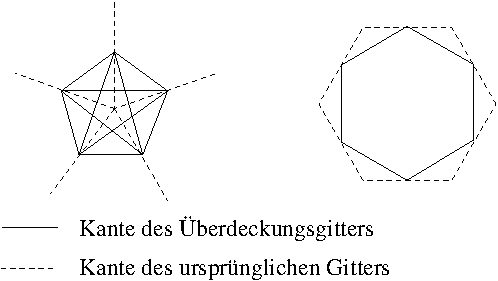
\includegraphics{./Schranken-figs/covering}
  \caption{Links: Der \"Uberdeckungsgraph eines Vertex mit Koordinationszahl $\bar{z}=5$ ist ein dekoriertes $\bar{z}$-Eck. Rechts: In jede Plakette des urspr\"unglichen Gitters wird eine undekorierte Plakette der gleichen Kantenzahl eingeschrieben.}
  \label{fig:covering}
\end{figure}
\\Wir betrachten bond-Perkolation auf einem archimedischen Gitter mit Vertexkonfiguration $(n_1,\ldots,n_{\bar{z}})$ und wollen die Euler-Charakteristik des \"Uberdeckungsgitter bestimmen. Die Euler-Charakteristiken der \"Uberdeckungsgitter werden zweckm\"a"siger\-weise mit der im Kapitel \ref{sec:matchingpoly} beschriebenen Methode f\"ur beliebige dekorierte Mosaike ausgerechnet. Um die Euler-Charakteristik zu bestimmen, m\"ussen wir die erwarteten Anzahlen der unterschiedlichen Vertextypen (siehe Abb. \ref{fig:decoratedcov}) kennen. 
\begin{figure}[htbp]
  \centering
  
\includegraphics{./Schranken-figs/decratedcov}
  \caption{Links ist ein Ausschnitt des Quadratgitters zu sehen, rechts ist der Wechselwirkungsgraph des \"Uberdeckungsgitters dieses Ausschnitts gezeigt. In alle Plaketten dieses Graphens, werden duale Spinvertices gesetzt.}
  \label{fig:decoratedcov}
\end{figure}
\begin{itemize}
\item Auf jeden Vertex von $G^{cov}$, d.h. auf jede Kante des archimedischen Gitters, wird ein Wechselwirkungsvertex $i\in I$ gesetzt. Diese Vertices sind mit Wahrscheinlichkeit $p$ besetzt.
\item Auf jede Kante des undekorierten Mosaiks von $G^{cov}$ werden Spinvertices $s \in S'$ gesetzt; diese Vertices sind immer vorhanden, werden aber nur gez\"ahlt, wenn mindestens einer der benachbarten Vertices aus $I$ besetzt ist. Das Mosaik hat Koordinationszahl $4$, und der Beitrag der Vertices aus $S'$ pro Wechselwirkungsvertex ist daher $2(1-(1-p)^2)=2(1-q^2)$.
\item In jede dekorierte Plakette von $G^{cov}$ wird ein Spinvertex $s\in S''$ gesetzt und mit allen umgebenden Wechselwirkungsvertices verbunden. Die Kantenzahl dieser Plaketten ist die Koordinationszahl $\bar{z}$ des archimedischen Gitters. Die Zahl dieser Plaketten verh\"alt sich zu der Zahl der Wechselwirkungsvertices wie die Zahl der Vertices zu der Zahl der Kanten des archimedischen Gitters. Wiederum werden Spins $s\in S''$ nur gez\"ahlt, wenn sie nicht isoliert sind. Der Beitrag der Vertices aus $S''$ pro Wechselwirkungsvertex ist daher $\frac{2}{\bar{z}}(1-(1-p)^{\bar{z}})=\frac{2}{\bar{z}}(1-q^{\bar{z}})$. Die Spinmenge $S$ aus Gleichung (\ref{eq:matchingpoly}) ist die Vereinigung aus $S'$ und $S''$.
\item In jede undekorierte Plakette wird ein dualer Spin $s^*\in S^{*'}$ gesetzt. Diese Plaketten entsprechen den Plaketten des archimedischen Gitters. Pro Vertex des archimedischen Gitters gibt es $\frac{1}{n_i}$ Plaketten mit Kantenzahl $n_i$, $i=1,\ldots,\bar{z}$; pro Wechselwirkungsvertex gibt es $\frac{2}{\bar{z}}$ Vertices des archimedischen Gitters und damit $\frac{2}{\bar{z}n_i}$ duale Spins $s^*\in S^{*'}$ pro Wechselwirkungsvertex, wiederum f\"ur $i=1,\ldots,\bar{z}$. Duale Spins werden gez\"ahlt, wenn sie nur von besetzten Wechselwirkungsvertices umgeben sind; Summation \"uber alle $i$ liefert den Beitrag $\sum_{i=1}^{\bar{z}}\frac{2}{\bar{z}n_i}p^{n_i}$.
\item Auch in die Dreiecke, die entstehen, wenn Spins $s\in S''$ mit den umliegenden Vertices aus $I$ verbunden werden, m\"ussen duale Spins $s^*\in S^{*''}$ gesetzt werden. Es gibt $\bar{z}$ dualer Spins $s^*$ pro Spin $s\in S''$ und damit zwei pro Wechselwirkungsvertex. Wenn beide Wechselwirkungsvertices auf den Ecken des Dreiecks besetzt sind, wird der Spin gez\"ahlt, und der Beitrag der dualen Spins aus $S^{*''}$ ist  $2p^2$.
\item Das Mosaik hat Koordinationszahl $4$; dar\"uberhinaus ist jeder Vertex aus $I$ mit zwei Vertices aus $S''$ verbunden und hat daher Koordinationszahl $6$.
\end{itemize}
Mit Gleichung (\ref{eq:matchingpoly}) und den eben bestimmten Gr\"o"sen erh\"alt man f\"ur die mittlere Euler-Charakteristik des \"Uberdeckungsgitter eines archimedischen Gitters mit Vertexkonfiguration $(n_1,\ldots,n_{\bar{z}})$
\begin{equation}
\label{eq:cov}
  \fbox{$\displaystyle \chi_{cov}(p)=p+2(1-q^2)+\frac{2}{\bar{z}}(1-q^{\bar{z}})+2p^2+\sum_{i=1}^{\bar{z}}\frac{2}{\bar{z}n_i}p^{n_i}-6p.$}
\end{equation}
Die Euler-Charakteristiken der \"Uberdeckungsgitter aller archimedischen Gitter, die Nullstellen und Wendepunkte der Euler-Charakteristiken und die bond-Perkolationsschwellen der archimedischen Gitter sind in Tabelle \ref{tab:covering} zusammengetragen. Die Perkolationsschwellen sind von van der Marck \cite{Marck:03} mit Genauigkeit $2*10^{-4}$ bestimmt worden. Um die entsprechenden Werte f\"ur die Laves-Gitter zu erhalten, muss $p$ durch $1-p$ ersetzt werden. Der Plot befindet sich wieder in Abbildung \ref{fig:2dallplots}. F\"ur bond-Perkolationsschwellen gilt, mit Ausnahme des $(3,4,6,4)$-Gitters, $p_0^{(2)}\leq p_c \leq p_0$ falls $p_c \geq \frac{1}{2}$ ist und $p_0^{(2)}\geq p_c \geq p_0$ falls $p_c \leq \frac{1}{2}$ ist.

\begin{table}
\centering
\begin{tabular}{|l|l||r|r|r||r|}
\hline
Vertexkon. & $\frac{\chi_{cov}(p)}{p(1-p)}$& $ p_0^{cov}$&$p_0^{(2)cov}$&$\frac{p_0^{cov}+p_0^{(2)cov}}{2}$&$p_c^{bond}$ \\ \hline
\hline
$3,12^2$ & $1-p-\frac{1}{9}\sum_{i=2}^{10}p^i $& $0.7580$&$0.6863$&$0.7221$&$0.7406(2)$ \\ \hline
$4,6,12$ & $1-p- \frac{2p^2+p^3+p^4}{6}-\frac{1}{18}\sum_{i=5}^{10}p^i $& $0.7054$&$0.6380$&$0.6717$&$0.6935(2)$ \\ \hline
$4,8^2$ & $1-p-\frac{1}{3}p^2-\frac{1}{6}\sum_{i=3}^6p^i $& $0.6964$&$0.6384$&$0.6674$&$0.6768(2)$ \\ \hline
$6^3$ & $1-p-\frac{1}{3}(p^2+p^3+p^4) $& $0.6756$&$0.6231$&$0.6494$&$0.65270\ldots$ \\ \hline
$3,6,3,6$ & $1-2p-\frac{1}{3}(p^2+p^3+p^4) $&$0.5277$&$0.5178$&$0.5228$&$0.5244053(3)$ \\ \hline
$3,4,6,4$ & $1-2p-\frac{1}{6}p^2-\frac{p^3+p^4}{12} $&$0.5134$&$0.5083$&$0.5109$&$0.5250(2)$ \\ \hline
$4^4$& $1-2p$&$0.5$&$0.5$&$0.5$&$0.5$ \\ \hline
$3^4,6$& $1-3p+\frac{1}{15}(23p^2-7p^3-p^4) $&$0.4069$&$0.4332$&$0.4200$&$0.4344(2) $ \\ \hline
$3^2,4,3,4$ & $1-3p+\frac{1}{5}(7p^2-2p^3) $&$0.3992$&$0.4305$&$0.4148$&$0.4142(2) $ \\ \hline
$3^3,4^2$ & $1-3p+\frac{1}{5}(7p^2-2p^3) $&$0.3992$&$0.4305$&$0.4148$&$0.4195(2) $ \\ \hline
$3^6$& $1-4p+\frac{1}{3}(10p^2-5p^3+p^4) $&$0.3244$&$0.3769$&$0.3506$&$0.34729\ldots$ \\ \hline
\end{tabular}
\caption{Euler-Charakteristik und bond-Perkolation auf archimedischen Gittern: Die erste Spalte enth\"alt die Vertexkonfiguration des archimedischen Gitters und die zweite die reduzierte mittlere Euler-Charakteristik des \"Uberdeckungsgitters $\frac{\chi^{cov}(p)}{p(1-p)}$. Bei fast allen Gittern mit bond-Perkolationsschwelle $p_c \geq \frac{1}{2}$ gilt f\"ur die Nullstelle $p_0$ und den Wendepunkt $p_0^{(2)}$ der Euler-Charakteristik $p_0^{(2)}\leq p_c \leq p_0$. F\"ur Gitter mit $p_c<\frac{1}{2}$ gilt $p_0^{(2)}\geq p_c \geq p_0$. Das Mittel aus $p_0$ und $p_0^{(2)}$ liegt nahe bei $p_c$. Die bond-Perkolationsschwellen des Dreiecks- ($3^6$), Sechsecks- ($6^3$) und Quadratgitters ($4^4$) sind exakt bekannt, der Wert f\"ur das Kagom\'egitter ($3,6,3,6$) stammt aus \cite{Suding:99}, alle \"ubrigen aus  \cite{Marck:03}. }
\label{tab:covering}
\end{table}

\begin{figure}[htbp]
  \centering
  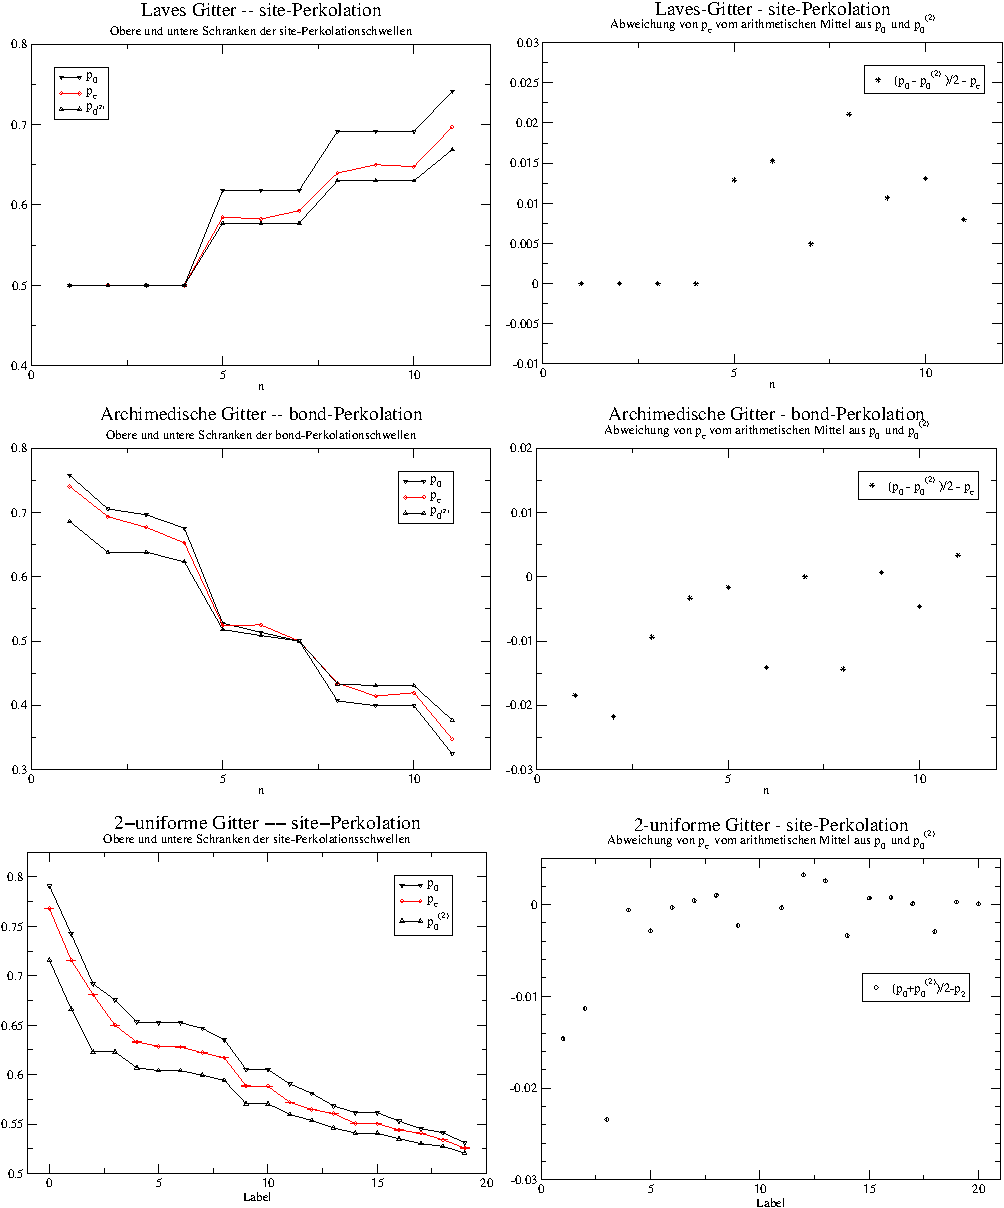
\includegraphics[width=16cm]{./Schranken-figs/2dallplots}
  \caption{In den drei Grafiken auf der linken Seite sind die Nullstellen $p_0$ und Wendepunkte $p_0^{(2)}$ der Euler-Charakteristiken, sowie die Perkolationsschwellen $p_c$ aller regelm\"a"sigen Gitter aufgetragen. In den drei rechten Grafiken ist die Abweichung des arithmetischen Mittels aus $p_0$ und $p_0^{(2)}$ von $p_c$ gezeigt. Die numerischen Werte sind in den Tabellen \ref{tab:covering}, \ref{tab:2-uniform} und \ref{tab:laves} zu finden. Der Plot f\"ur site-Perkolation archimedischer Gitter ist in Abb. \ref{fig:archisite} zu finden.}
  \label{fig:2dallplots}
\end{figure}
\subsection{Irregul\"are Gitter}
Es gibt einige weitere Gitter, deren site-Perkolationsschwellen bekannt sind, die aber nicht in die oben behandelten Kategorien passen. Daher werden sie hier gesondert vorgestellt.\\
Das Bowtie-Gitter hat Vertexkonfiguration $\left[ \frac{1}{2}(4,3,4,3)_1+\frac{1}{2}(4,3^2,4,3^2)_2 \right]$; sein duales Gitter $\left[ \frac{2}{3}(4,6^2)_1+\frac{1}{3}(4,6,4,6)_2 \right]$ (siehe Abb. \ref{fig:bowtie}). F\"ur die Euler-Charakteristiken erh\"alt man mit Gleichung (\ref{eq:2-uniform})
\begin{eqnarray}
  \chi(p) & = &p(1-p)\left(1-\frac{3}{2}p-\frac{1}{2}p^2 \right)\\
 \chi^{dual}(p)& = & p(1-p)\left(1-\frac{2p+2p^2+p^3+p^4}{3} \right).
\end{eqnarray}
\begin{figure}[bp]
  \centering
  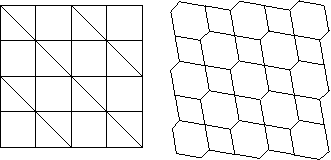
\includegraphics{./Schranken-figs/bowtie}
  \caption{Bowtie- (links) und duales Bowtie-Gitter}
  \label{fig:bowtie}
\end{figure}
\\Das Penrose-Gitter ist ein nichtperiodisches Gitter, dessen Plaketten alle Vierecke sind \cite{Gruenbaum:86}. Seine mittlere Euler-Charakteristik ist daher die gleiche wie beim Quadratgitter.\\
Auch f\"ur die zuf\"alligen Delauny- und Voronoi-Gitter \cite{Weygaert:91} l\"asst sich in zwei Dimensionen die mittlere Euler-Charakteristik bestimmen. Das Delauny-Gitter besteht nur aus Dreiecken und die Euler-Charakteristik ist $\chi^{delauny}(p)=p(1-p)(1-2p)$. Die Euler-Charakteristik des Voronoi-Gitters h\"angt von der Verteilung $s_n$ der Plaketten mit Kantenzahl $n$ ab, die aber nur approximativ bekannt ist. Der Mittelwert der Kantenzahl ist $6$ und die Koordinationszahl fast sicher $z=3$. Damit erh\"alt man 
\begin{equation}
\label{eq:voronoi}
  \chi^{Voronoi}(p)=p-1+\frac{3}{2}(1-p^2)-\frac{1}{2}\sum_{n\geq 3}s_n(1-p^n).
\end{equation}
Das \"Uberdeckungsgitter des Voronoi-Gitters entspricht einem Kagom\'e-Gitter, in dem die Sechsecke durch unregelm\"a"sige Polygone ersetzt sind. Die Kantenzahl der unregelm\"a"sigen Polygone hat die Verteilung $s_n$, und die Euler-Charakteristik ist mit Gl. (\ref{eq:cov}) 
\begin{equation}
\label{eq:voronoibond}
  \chi^{Vor.cov.}(p) =  p+2(1-q^2)+\frac{2}{3}(1-q^3)-6p+2p^2+\frac{2}{3}\sum_{n\geq 3}s_np^n.
\end{equation}
Die Werte der Perkolationsschwellen $p_c$ der Gitter, sowie der Nullstellen $p_0$ und Wendepunkte $p_0^{(2)}$ der Euler-Charakteristiken sind in Tabelle \ref{tab:irreg} zusammengetragen. In allen F\"allen gilt $p_0\geq p_c \geq p_0^{(2)}$. Steven van der Marck \cite{Marck:03} hat noch f\"ur eine Reihe weiterer Gitter Perkolationsschwellen bestimmt. Viele dieser Gitter enthalten aber Substrukturen und zeigen die Grenzen der G\"ultigkeit der Faustregel auf. Auf diese Gitter wird im n\"achsten Kapitel genauer eingegangen.\\
\begin{table}
\centering
\begin{tabular}{|l|r|r|r||r|}
\hline
Name &  $ p_0$&$p_0^{(2)}$&$\frac{p_0+p_0^{(2)}}{2}$&$p_c$ \\ \hline
\hline
bowtie & $0.5616$ &$0.5408$&$0.5512$&$0.5474(8)$\cite{Marck:97} \\ \hline
bowtie dual & $0.7048$&$0.6411$&$0.6730$&$0.6653(6)$\cite{Marck:97} \\ \hline
Penrose &  $0.6180$&$0.5774$&$0.5977$&$0.5837(2)$\cite{Yonezawa:88} \\ \hline
Delauny & $1/2$ & $1/2$ & $1/2$&$1/2$ \\ \hline
Voronoi &$0.7548$&$0.6787$&$0.7167$&-- \\ \hline
Voronoi bond  & $0.6855$&$0.6288$&$0.6572$&$0.6670(1)$\cite{Hsu:99}  \\ \hline
\end{tabular}
\caption{Perkolation und Euler-Charakteristik unregelm\"a"siger Gitter: F\"ur die Nullstellen $p_0$ und die Wendepunkte $p_0^{(2)}$ der Euler-Charakteristiken und die Perkolationsschwellen $p_c$ gilt $p_0^{(2)}\leq p_c\leq p_0$. Das Mittel aus $p_0$ und $p_0^{(2)}$ ist nahe bei $p_c$. Abgesehen von der Zeile ``Voronoi bond'', beziehen sich alle Werte auf site-Perkolation. Um $p_0$ und $p_0^{(2)}$ des Voronoi-Gitters zu erhalten, wurde eine approximative Verteilung $s_n$ der Plaketten mit Kantenzahl $n$ aus \cite{Stoyan:96} verwendet.}
\label{tab:irreg}
\end{table}


\subsection{Zuf\"allig dekorierte Mosaike}
\label{sec:decorated}
Ein Gitter heisst dekoriertes Mosaik, wenn es aus einem planaren Gitter (Mosaik) besteht, dessen Plaketten teilweise um allen diagonalen Kanten erweitert wurden. Die Vertices auf dem Rand einer solchen Plakette sind dann alle durch Kanten verbunden, und die Plakette heisst dekoriert (siehe Kapitel \ref{sec:dualitaet}). Um zu untersuchen, wie sich $p_c$ mit dem Bruchteil der dekorierten Plaketten eines Mosaiks \"andert, kann man Gitterplaketten mit Wahrscheinlichkeit $m$ dekorieren, und $p_c$ f\"ur eine Reihe verschiedener Werte von $m$ bestimmen. Die mittlere Euler-Charakteristik dieser statistisch dekorierten Mosaike kann mit Gl. (\ref{eq:matchingpoly}) bestimmt werden. Dazu m\"ussen die Kardinalit\"aten der Vertexmengen und die mittlere Koordinationszahl des Wechselwirkungsgraphs (siehe Abb. \ref{fig:randomdec}) bestimmt werden. 
\begin{figure}[bp]
  \centering
  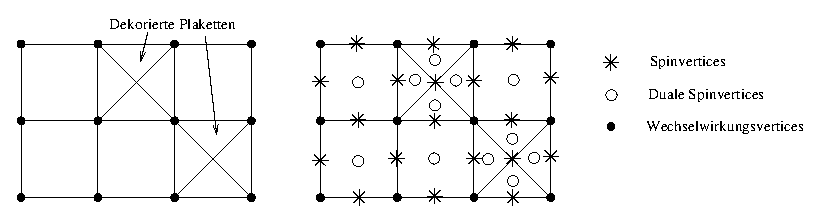
\includegraphics{./Schranken-figs/randomdec}
  \caption{Teil eines dekorierten Quadratgitters (links) und der resultierende Wechselwirkungsgraph (rechts).}
  \label{fig:randomdec}
\end{figure}
\begin{itemize}
\item Wechselwirkungsvertices sitzen auf jedem Gitterplatz und sind mit Wahrscheinlichkeit $p$ besetzt.
\item Spinvertices $s\in S$ sitzen auf allen Kanten und in dem mit Wahrscheinlichkeit $m$ dekorierten Plaketten. Wenn das Mosaik nur Plaketten mit Kantenzahl $n$ und Vertices mit Koordinationszahl $z$ hat, gibt es pro Wechselwirkungsvertices im Mittel $\frac{z}{2}(1-(1-p)^2)+m\frac{z}{n}(1-(1-p)^n)$ Spins. Bei einem komplizierteren Gitter treten mehr Terme auf, die aber analog berechnet werden k\"onnen.
\item Duale Spinvertices $s^*\in S^*$ werden in alle undekorierten Plaketten und in die Dreiecke, in die die dekorierten Plaketten durch den Wechselwirkungsgraph zerschnitten werden, gesetzt. Sie werden nur dann gez\"ahlt, wenn alle umliegenden Wechselwirkungsvertices besetzt sind. Haben alle Plaketten Kantenzahl $n$, gibt es pro Wechselwirkungsvertex $(1-m)\frac{z}{n}p^n+mzp^2$ duale Spins.
\item Die Koordinationszahl eines Wechselwirkungsvertex ist die des Mosaiks $z$, zuz\"uglich der Zahl der ihn umgebenden dekorierten Plaketten. Die mittlere Koordinationszahl ist $\bar{z}=z+\sum_{i=1}^z im^i(1-m)^{z-i}{ i \choose z }$.
\end{itemize}    
Mit Gleichung (\ref{eq:matchingpoly}) und den oben bestimmten Gr\"o"sen l\"asst sich die Euler-Charakteristik ausrechen.
\\Die Perkolationsschwellen komplement\"ar dekorierter Mosaike erg\"anzen sich zu 1. F\"ur $m=1/2$ sind die zuf\"allig dekorierten Mosaike im statistischen Sinn selfmatching, und $p_c$ sowie $p_0$ sind $1/2$. Perkolation auf zuf\"allig dekorierten Gittern ist eine Form der gemischten Perkolation. Vertices werden mit Wahrscheinlichkeit $p$ und Plaketten mit Wahrscheinlichkeit $m$ besetzt. Kanten sind immer besetzt.\\
Ich habe f\"ur das Quadrat-, Sechseck- und Kagom\'e-Gitter, sowie das $3^3,4^2$- und das $3,12^2$-Gitter die Perkolationsschwelle in Abh\"angigkeit von $m$ berechnet. Details der Simulation sind im Anhang \"uber numerische Methoden zusammengefasst. Die Perkolationsschwelle f\"allt vom leeren zum vollst\"andig dekorierten Mosaik ab (siehe Abb. \ref{fig:dekoratedpc}). Die Perkolationsschwellen von Gittern mit einem Anteil an dekorierten Plaketten von $m\in[0,1]$ und $1-m$ erg\"anzen sich zu $1\pm 0.01$, wie aufgrund der statistischen matching-Eigenschaft zu erwarten war. Die Genauigkeit der Simulation ist nicht sehr hoch, da f\"ur jedes Gitter 100 verschiedene Werte von $m$ simuliert werden mussten. Die Fehlerabsch\"atzungen ergeben sich einfach aus den Fluktuationen von $p_c(m)$ um eine glatte Kurve.
\begin{figure}[htbp]
  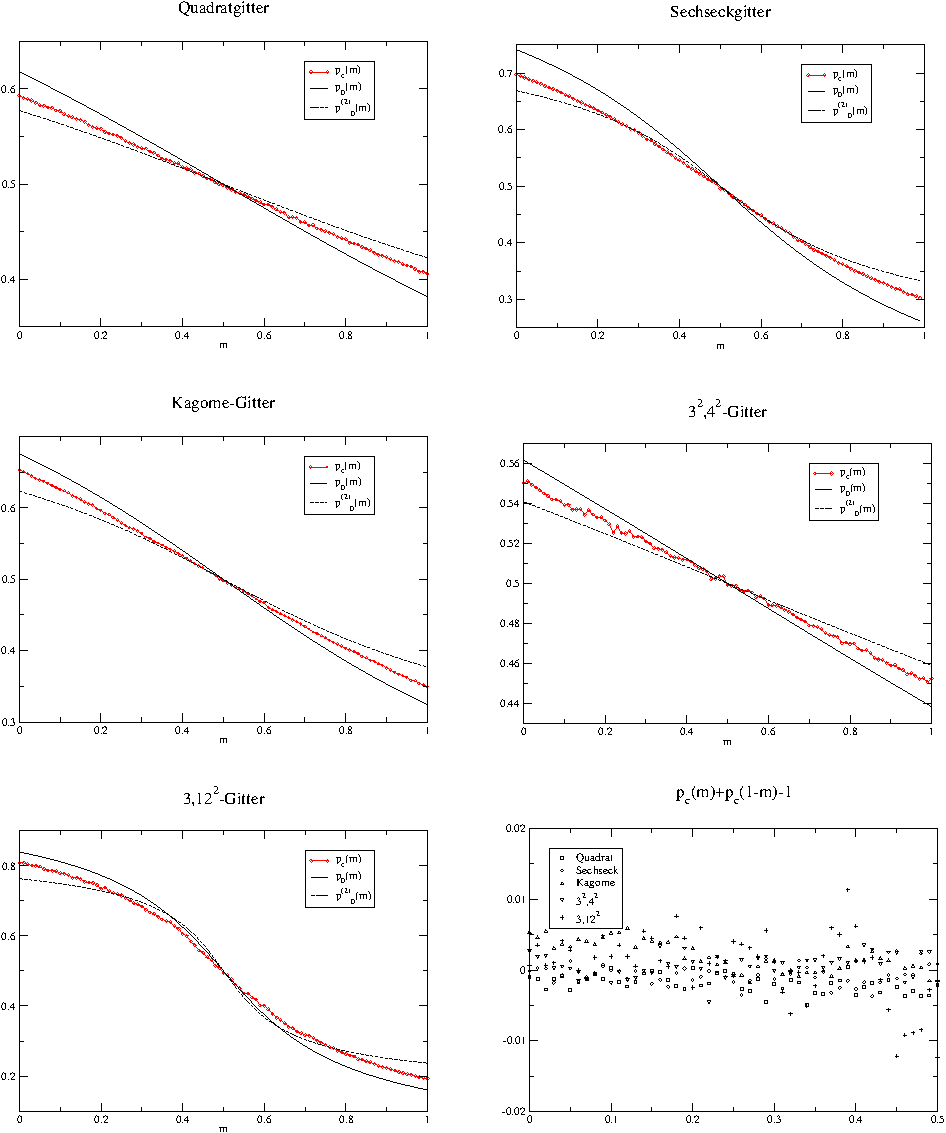
\includegraphics{./Schranken-figs/matching}
  \caption{Die Grafiken zeigen die Perkolationsschwelle $p_c(m)$ in Abh\"angigkeit vom Bruchteil $m$ der dekorierten Plaketten f\"ur die f\"unf untersuchten Gitter. Zus\"atzlich sind Nullstelle $p_0(m)$ und Wendepunkt $p_0^{(2)}(m)$ der Euler-Charakteristik eingezeichnet. Rechts unten ist die Abweichung von $p_c(m)+p_c(1-m)$ von $1$ f\"ur alle Gitter aufgetragen.}
\label{fig:dekoratedpc}
\end{figure}
\begin{figure}[htbp]
  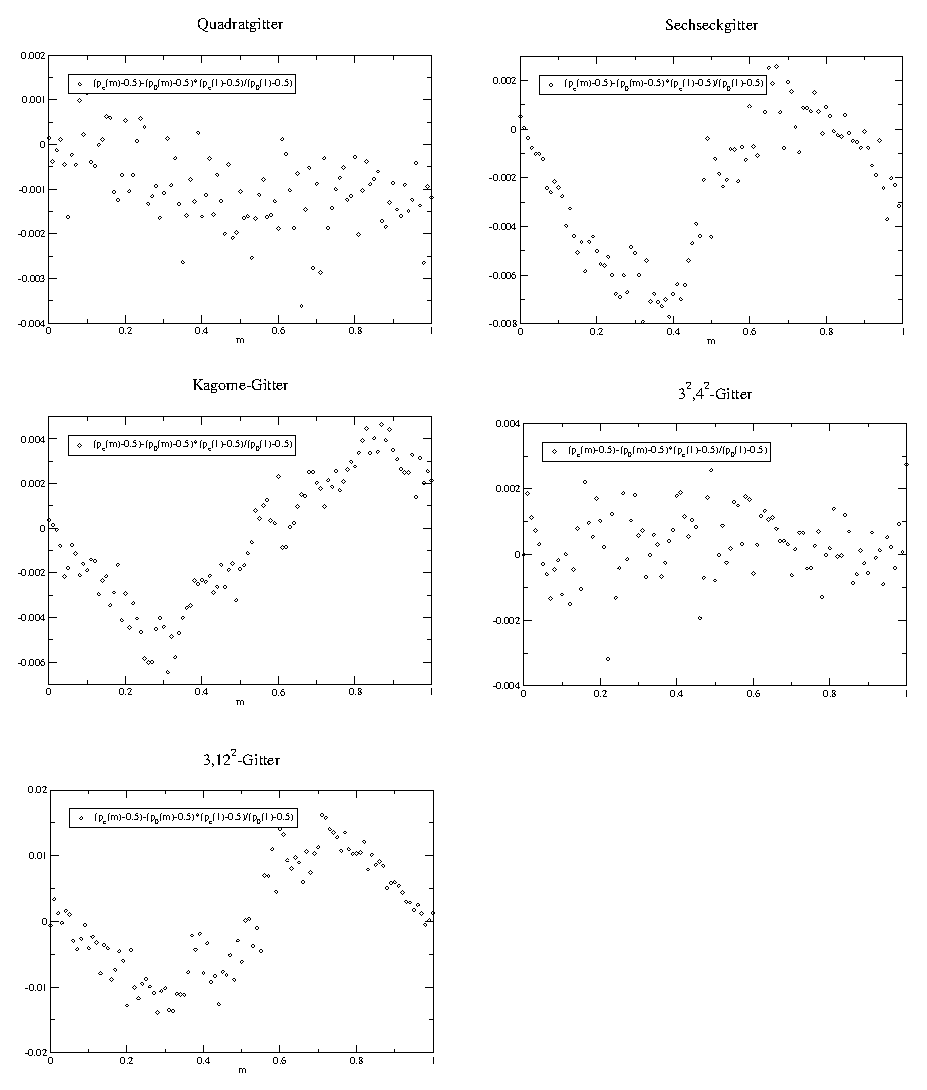
\includegraphics{./Schranken-figs/scale}
  \caption{Die Perkolationsschwelle $p_c(m)$ von Gittern, deren Plaketten mit Wahrscheinlichkeit $m$ dekoriert sind, ist fast identisch mit der reskalierten Nullstelle der Euler-Charakteristik $(p_0(m)-0.5)\frac{p_c(1)-0.5}{p_0(1)-0.5}+0.5$. F\"ur die f\"unf untersuchten Gitter ist die Differenz beider Gr\"o"sen aufgetragen.}
\label{fig:scale}
\end{figure}
\\W\"ahrend f\"ur Gitter mit Perkolationsschwellen nahe $\frac{1}{2}$ die Kurve $p_c(m)$ kaum von einer Geraden abweicht, ist beim Sechseck- und $3,12^2$-Gitter ein geschwungener Verlauf deutlich erkennbar (siehe Abb. \ref{fig:dekoratedpc}). F\"ur alle Gitter und alle $m$ ist die Nullstelle der Euler-Charakteristik im Rahmen der Genauigkeit der Simulation f\"ur $p_c<\frac{1}{2}$ eine untere und f\"ur $p_c>\frac{1}{2}$ eine obere Schranke. F\"ur den Wendepunkt der Euler-Charakteristik gilt das komplement\"are Verhalten, anders als f\"ur $m=0$ und $m=1$, nicht. Die Kurve $p_0(m)$ hat sehr \"ahnliche Form wie $p_c(m)$, und beide Kurven k\"onnen durch Skalierung fast zur Deckung gebracht werden. In Abbildung \ref{fig:scale} ist die Differenz von $p_c(m)$ und $(p_0(m)-0.5)\frac{p_c(1)-0.5}{p_0(1)-0.5}+0.5$ f\"ur die untersuchten Gitter dargestellt. Die Abweichung liegt innerhalb der Fehlergrenzen der Simulation, zeigt aber f\"ur Gitter mit gro"sem $p_c$ systematische Variation.\\
Die Daten stimmen innerhalb der Fehlergrenzen mit bekannten Perkolationsschwellen f\"ur undekorierte oder vollst\"andig dekorierte Gitter \"uberein \cite{Suding:99}.


\section{Euler-Charakteristik gro"ser Cluster}
\label{sec:scaling}
Bei allen bisher untersuchten zweidimensionalen Gitter, mit Ausnahme der bond-Perkolation auf dem $(3,4,6,4)$-Gitter, ist $p_0$ gr\"o"ser als $p_c$, wenn $p_c>\frac{1}{2}$, und kleiner, wenn $p_c<\frac{1}{2}$ ist. Auch die Untersuchungen an zuf\"allig dekorierten Gitter haben die Vermutung sehr gut best\"atigt, dass $p_0>p_c$ ist, falls $p_c>\frac{1}{2}$ ist, und, dass $p_0<p_c$ ist, falls $p_c<\frac{1}{2}$ ist. Zusammen mit den archimedischen Gittern ist die vermutete Beziehung zwischen $p_0$ und $p_c$ also auf einer gro"sen Zahl von Gittern, wenn auch nur numerisch, verifiziert worden. Im Folgenden soll der Versuch gemacht werden, die Ursache dieses Sachverhalts zu verstehen.\\

An der Perkolationsschwelle divergiert die Korrelationsl\"ange und es gibt, abgesehen von der Gitterkonstanten, keine charakteristische L\"angenskala. Die Skalenannahme sagt voraus, dass die Clusterkonfiguration auf jeder Skala, die gro"s gegen den Gitterabstand ist, qualitativ gleich aussieht. Stauffer \cite{Stauffer:95} hat f\"ur die Zahl der Cluster pro Vertex $n_s$ der Gr\"o"se $s$ in der N\"ahe von $p_c$ ($\Delta p=p-p_c$)
\begin{equation}
  \label{eq:skalenann}
   n_s=q_0 s^{-\tau}f(\Delta pq_1s^{\sigma})
\end{equation}
als Skalenrelation vorgeschlagen. Die Parameter $q_0,q_1$ und $p_c$ h\"angen vom betrachteten Gitter ab; die \"ubrigen Gr\"o"sen und die Funktion $f(z)$ sind universell.\\
Seien nun $q_0,q_1$ und $p_c$ die nicht-universellen Parameter des betrachteten Gitters und $q_0^*,q_1^*$ und $1-p_c$ die des matching Gitters. Die Summen
\begin{equation}
  \sum_{s=s_0}^{\infty}n_s(p) \qquad \text{und} \qquad \sum_{s=s_0}^{\infty}n_s^*(q)
\end{equation}
sind die Zahlen der Cluster bzw. L\"ocher, die gr\"o"ser als ein gewisses $s_0$ sind. Ihre Differenz ist die Euler-Charakteristik pro Vertex, zu der nur Cluster der Gr\"o"se $s\geq s_0$ beitragen. Mit der Skalenannahme ergibt sich
\begin{equation}
   \chi_{s_0}(p):=\sum_{s=s_0}^{\infty}n_s(p)-n_s^*(1-p)=\sum_{s=s_0}^{\infty}s^{-\tau}\left[ q_0f(\Delta pq_1s^{\sigma})-q_0^*f(-\Delta pq_1^*s^{\sigma})\right].
\end{equation}
Die Wahrscheinlichkeiten, dass ein Vertex in einem Cluster oder einem Loch der Gr\"o"se $s\geq s_0$ ist, sind durch 
\begin{equation}
  \sum_{s=s_0}^{\infty}sn_s(p)+P_{\infty}(p) \qquad \text{und} \qquad \sum_{s=s_0}^{\infty}sn_s^*(q)+P_{\infty}^*(q)
\end{equation}
gegeben.
F\"ur die Differenz beider Gr\"o"sen gilt mit der Skalenannahme
\begin{equation}
\begin{split}
   [p-q]_{s_0}& :=\sum_{s=s_0}^{\infty}s\left[n_s(p)-n_s^*(1-p)\right]+P_{\infty}(p)-P_{\infty}^*(q) \\ & =\sum_{s=s_0}^{\infty}s^{-\tau+1}\left[ q_0f(\Delta pq_1s^{\sigma})-q_0^*f(-\Delta pq_1^*s^{\sigma})\right]+P_{\infty}(p)-P_{\infty}^*(q).
\end{split}
\end{equation}
Bei $p=p_c$ vereinfachen sich die Beziehungen zu 
\begin{equation}
   \chi_{s_0}(p_c)=(q_0-q_0^*)f(0)\sum_{s={s_0}}^{\infty}s^{-\tau}
\end{equation}
und 
\begin{equation}
   [p_c-q_c]_{s_0}=(q_0-q_0^*)f(0)\sum_{s=s_0}^{\infty}s^{-\tau+1}.
\end{equation}
Die Summen lassen sich durch Integrale n\"ahern und man erh\"alt
\begin{equation}
   \chi_{s_0}(p_c)=(q_0-q_0^*)f(0)\frac{s_0^{-\tau+1}}{\tau-1}
\end{equation}
und
\begin{equation}
   [p_c-q_c]_{s_0}=(q_0-q_0^*)f(0)\frac{s_0^{-\tau+2}}{\tau-2}.
\end{equation}
Der Exponent $\tau$ hat in zwei Dimensionen vermutlich den Wert $\frac{187}{91}$, ist also gr\"o\ss er als $2$. Daher haben $\chi_{s_0}(p_c)$ und $[p_c-q_c]_{s_0}$ das gleiche Vorzeichen und ihr Verh\"altnis ist
\begin{equation}
   \fbox{$\displaystyle \frac{\chi_{s_0}(p_c)}{[p_c-q_c]_{s_0}}=\frac{\tau-2}{\tau-1}s_0^{-1}=\frac{5}{96s_0}.$}
\end{equation}
Wenn sich das Skalenverhalten bis zu kleinen Clustern qualitativ fortsetzt, ist $\chi(p_c)$ positiv und das Verh\"altnis $\frac{\chi(p_c)}{p_c-q_c}$ sollte ungef\"ahr $\frac{5}{96}$ betragen. F\"ur archimedische Gitter gilt dies im Rahmen der Erwartungen (siehe Tabelle \ref{tab:archiscale}).
\begin{table}
\centering
\begin{tabular}{|l|r|r|}
\hline
Gitter &$\frac{\chi(p_c)}{p_c-q_c}$ ($s_0=1$) &$\frac{\chi(p_c)}{p_c-q_c}-\frac{5}{96}$ \\
\hline
$3,12^2$ & $ 0.0284$&$-0.0237$\\
$4,6,12$ & $ 0.0381$&$-0.0140$\\
$4,8^2$ &$0.0478$&$-0.0043$\\
Sechseckg.&$0.0649$&$0.0128$ \\
Kagom\'eg. &$0.0387$&$-0.0134$\\
$3,4,6,4$&$ 0.0534$&$0.0014$ \\
Quadratg. &$0.0727$&$0.0207$\\
$3^3,6$ &$0.0361$&$-0.0160$\\
$3^2,4,3,4$ &$ 0.0538$&$0.0017$\\
$3^3,4^2$ &$0.0574$ &$0.0054$\\
Dreiecksg. &-- &--\\\hline
\end{tabular}
\caption{Euler-Charakteristik archimedischer Gitter bei $p=p_c$.}
\label{tab:archiscale}
\end{table}
\\F\"ur das Quadratgitter sind die Clusterzahlen sowohl f\"ur n\"achste, als auch f\"ur \"ubern\"achste Nachbarschaften bis $s=12$ bekannt \cite{Mertens:90}, und $\chi_{s_0}(p_c)$ sowie $[p_c-q_c]_{s_0}$ k\"onnen durch Abziehen der bekannten Beitr\"age der Cluster $s<s_0$ von $\chi(p_c)$ und $[p_c-q_c]=2p_c-1$ berechnet werden. Schon f\"ur $s_0\geq 3$ lassen sich die so gewonnen Werte gut an ein Potenzgesetz fitten (siehe Abb. \ref{fig:analytisch_pc_fig}). Die Werte der Fitparameter stimmen aber nur m\"a"sig mit den Erwartungen \"uberein.
\begin{figure}[tbp]
  \centering
  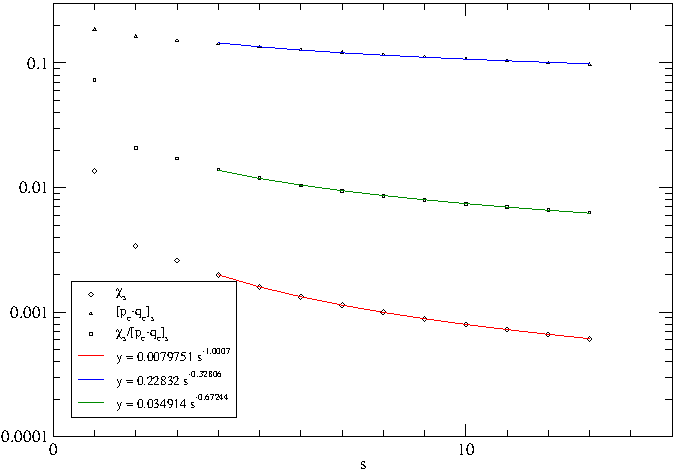
\includegraphics{./Schranken-figs/analytisch_pc_fig}
  \caption{Euler-Charakteristik $\chi_s(p_c)$ und $[p_c-q_c]_s$ (siehe Text) auf dem Quadratgitter f\"ur $s=1,\ldots,13$. Die Kurven sind Fitkurven an die Werte $s\geq3$. Zur Vereinfachung der Darstellung hat der Plot eine logarithmische Ordinate.}
  \label{fig:analytisch_pc_fig}
\end{figure}
\\Da die Clusterzahlen f\"ur gro"ser Cluster nicht exakt bekannt sind, m\"ussen Resultate f\"ur gr\"o"sere $s_0$ aus Monte-Carlo-Simulationen gewonnen werden. Hierzu wird mit dem im Appendix \ref{sec:numerik} vorgestellten Programm eine Perkolationskonfiguration erzeugt und die Clusterverteilung (siehe Abschnitt \ref{sec:numerikverteilung}) ausgewertet. Die Simulationen wurden f\"ur site-Perkolation auf dem Quadrat- und Sechseckgitter sowie f\"ur bond-Perkolation auf dem Sechseckgitter durchgef\"uhrt. Die Kantenl\"ange der simulierten Gitter betrug $L=2048$. Die Ergebnisse sind in sehr guter \"Ubereinstimmung mit dem erwarteten Skalenverhalten. Auch die numerischen Werte f\"ur die Exponenten und das Verh\"altnis $\frac{\chi_{s_0}(p_c)}{[p_c-q_c]_{s_0}}$ stimmen sehr gut mit den Vorhersagen der Skalenannahme \"uberein. Die gewonnen Daten und die ermittelten Fitparameter sind in Abb. \ref{fig:scalinglimit} dargestellt.\\
\begin{figure}[htbp]
  \centering
  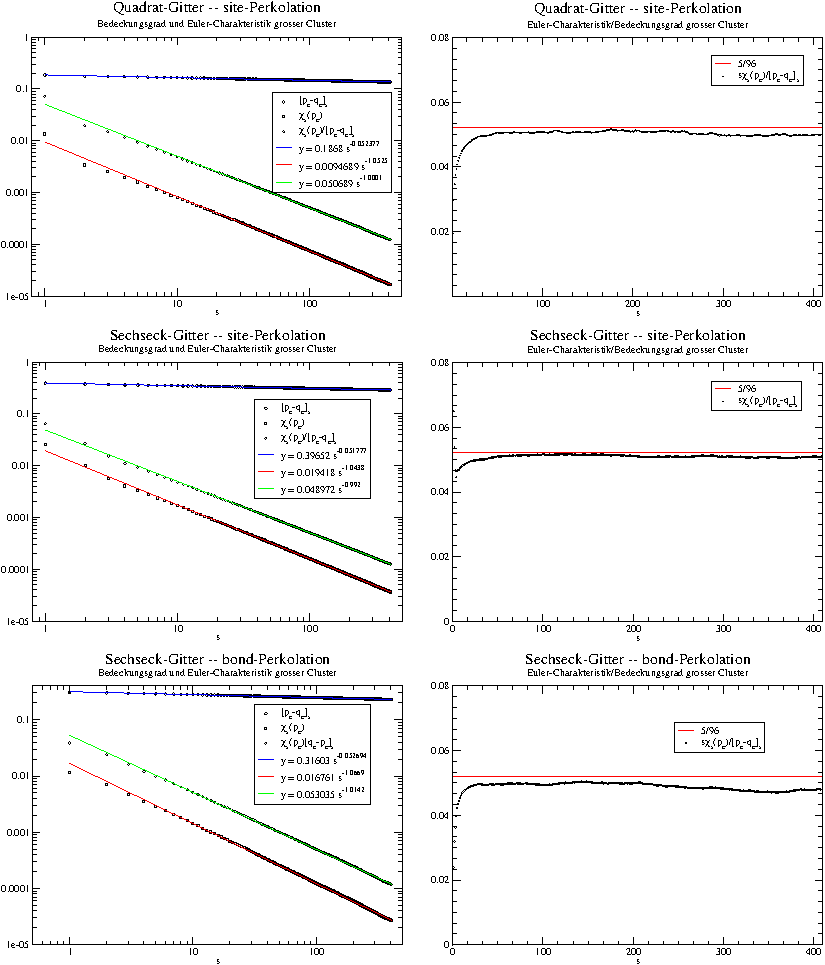
\includegraphics{./Schranken-figs/scalinglimit}
  \caption{Simulationsergebnisse f\"ur die Clusterverteilung bei $p_c$ der site-Perkolation auf dem Quadrat- und Sechseckgitter, sowie bond-Perkolation auf dem Sechseckgitter. Auf der linken Seite sind $\chi_s$, $\chi_s/[p_c-q_c]_s$ und $[p_c-q_c]_s$ doppelt-logarithmisch aufgetragen. Rechts  ist $s\chi_s/[p_c-q_c]_s$ und das erwartete Skalenverhalten $5/96$ dargestellt.}
  \label{fig:scalinglimit}
\end{figure}

Mit der Skalenannahme aus Gleichung (\ref{eq:skalenann}) kann auch die Nullstelle von $n_s(p)-n_s^*(1-p)$ f\"ur gro"se $s$ durch die nicht-universellen Parameter der Gitter ausgedr\"uckt werden. 
\begin{equation}
      n_s(p)-n_s^*(1-p)=q_0 s^{-\tau}f((p-p_c)q_1s^{\sigma})-q_0^* s^{-\tau}f((p_c-p)q_1^*s^{\sigma}).
\end{equation}
F\"ur die Nullstelle von $n_s(p)-n_s^*(1-p)$ ergibt sich die Bedingung ($\Delta p=p_0-p_c$)
\begin{equation}
      q_0 s^{-\tau}f(\Delta p q_1s^{\sigma})=q_0^* s^{-\tau}f(-\Delta p q_1^*s^{\sigma}).
\end{equation}
Angenommen $f(z)$ l\"asst sich um $z=0$ entwickeln, erh\"alt man
\begin{equation}
\begin{split}
 & q_0(f(0)+f'(0)\Delta p q_1s^{\sigma}+\frac{1}{2}f''(0)(\Delta p q_1s^{\sigma})^2+\ldots) \\ & =  q_0^* (f(0)-f'(0)\Delta p q_1^*s^{\sigma}+\frac{1}{2}f''(0)(\Delta p q_1^*s^{\sigma})^2+\ldots).
\end{split}
\end{equation}
Nach Potenzen in $\Delta p s^\sigma$ geordnet ergibt sich
\begin{equation}
  f(0)(q_0-q_0^*)+f'(0)(q_0q_1+q_0^*q_1^*)\Delta p s^\sigma+\frac{1}{2}f''(0)(q_0q_1^2-q_0^*{q_1^{*}}^2)(\Delta ps^{\sigma})^2+\ldots=0.
\end{equation}
$\Delta p s^\sigma$ muss f\"ur alle $s$ L\"osung des Polynoms mit konstanten Koeffizienten sein. F\"ur die L\"osung gilt $\Delta p s^\sigma=const.$ oder $\Delta p=const.* s^{-\sigma}$. Falls $\Delta ps^\sigma \ll 1$, kann man Terme h\"oherer Ordnung vernachl\"assigen. Eine konsistente Skalenfunktion $f(x)$ hat ihr einziges Maximum bei negativem $x$ \cite{Stauffer:95}, und daher ist $f'(0)<0$. $\Delta p$ hat dann das gleiche Vorzeichen wie $q_0-q_0^*$ und ist mit obigen Argumenten f\"ur $p_c>1/2$ positiv. Die bekannten Clusterzahlen f\"ur das Quadratgitter best\"atigen das Skalenverhalten, und ein Fit an die Werte $s=6,\ldots,12$ liefert einen Exponenten $\sigma=0.38$. Es wird vermutet, dass $\sigma$ den Wert $\frac{36}{91}\approx 0.396$ hat. \\ 

Mit der Skalenhypothese l\"asst sich die Beobachtung, dass f\"ur $p_c>\frac{1}{2}$ die Nullstelle der Euler-Charakteristik \"uber $p_c$ liegt, begr\"unden. Allerdings liefern kleine Cluster mit Abstand den gr\"o"sten Beitrag zur Euler-Charakteristik und gerade f\"ur diese ist die Skalenannahme nicht g\"ultig. Wenn sich das Skalenverhalten qualitativ auf kleine Cluster fortsetzt, sollte aber $p_c<p_0$ gelten, wenn $p_c>\frac{1}{2}$ ist.  

\section{Euler-Charakteristiken in drei Dimensionen}
Um den Zusammenhang zwischen $p_0$ und $p_c$ in drei Dimensionen weiter zu untersuchen, wurde die mittlere Euler-Charakteristik verschiedener dreidimensionaler Gitter berechnet, deren Perkolationsschwellen bekannt sind. Wie schon im Kapitel \ref{sec:chimittel} diskutiert, m\"ussen zur Berechnung der Euler-Charakteristik von Clustern auf dreidimensionalen Gittern, Zellen um die Vertices gefunden werden, die die Nachbarschaftsverh\"altnisse des Gitters widerspiegeln. Die Wahl solcher Zellen ist in der Regel nicht eindeutig. Bei Gittern, deren Wigner-Seitz-Zellen (WSZ) geeignet sind, um die Euler-Charakteristik zu berechnen, sind die WSZ als nat\"urliche Zellen vorgegeben. Dennoch kann man auch durch Wahl anderer Zellen Zusammenhangsverh\"altnisse erzeugen, die denen des Gitters entsprechen. Die Zahl der Zellen, mit denen eine Zelle einen nichtleeren Durchschnitt hat, ist bei diesen Zellen aber i. A. eine andere als bei den WSZ, und man erh\"alt unterschiedliche Euler-Charakteristiken. 
\\Sind geeignete Zellen gefunden, werden sie wie immer mit Wahrscheinlichkeit $q=1-p$ besetzt. Wir berechnen die mittlere Euler-Charakteristik dieser Figuren $\bar{\chi}(1-p)$. In drei Dimensionen gilt f\"ur die Euler-Charakteristik des geeignet abgeschlossenen Komplements $\chi(p)=\bar{\chi}(1-p)$. Wir werden uns auf Ergebnisse und wesentliche Aspekte beschr\"anken und technische Details der Rechnungen und Konstruktionen in den Appendix verbannen.

\subsection{Gitterstapel}
Die einfachste M\"oglichkeit dreidimensionale Gitter zu erhalten, ist, Ebenen zweidimensionaler Gitter \"ubereinander zu legen, und jeden Vertex mit den Vertices \"uber und unter ihm zu verbinden. Solche Gitter hei"sen Gitterstapel.\\
Prismen mit den dualen Plaketten der zweidimensionalen Gitter als Grundfl\"ache sind geeignete Zellen, um die Euler-Charakteristik auszurechnen. Die H\"ohe der Prismen ist der Gitterebenenabstand, und die Gittervertices sollen im Schwerpunkt der Prismen liegen. Diese Prismen haben nur mit den Prismen der n\"achsten Nachbarn im zweidimensionalen Gitter und mit denen der senkrecht \"uber und unter ihnen liegenden Gittervertices eine Fl\"ache gemein. Sie sind daher geeignet $\chi(p)$ zu berechnen. \\
Durch die Gitterebenen ist eine Schichtstruktur vorgegeben und die Euler-Charakteristik wird zweckm\"a"sigerweise mit der Schnittrekursion ausgerechnet. Die Schnittebenen stehen senkrecht auf Symmetrieachse der Prismen. Das Schnittmuster besteht aus besetzten und unbesetzten dualen Plaketten des zweidimensionalen Gitters. Die mittlere Euler-Charakteristik dieser Muster ist die des vollst\"andig dekorierten zweidimensionalen Gitters $\bar{\chi}_{2}(q)$. Die Schnittmuster \"andern sich nur, wenn die Schnittebene von einer Prismenschicht in die n\"achste wandert. Dort, wo sich zwei Prismenschichten ber\"uhren, sind die Plaketten des Schnittmusters mit Wahrscheinlichkeit $1-(1-q)^2$ besetzt. Jeder andere Schnitt entspricht dem zweidimensionalen Gitter mit Besetzungswahrscheinlichkeit $q$. Die Differenz der Euler-Charakteristiken beider Schnitte ist $\bar{\chi}(q)$:
\begin{equation}
  \bar{\chi}(q)=\bar{\chi}_{2}(1-(1-q)^2)-\bar{\chi}_{2}(q).
\end{equation}
In zwei Dimensionen gilt $\chi_2(p)=-\bar{\chi}_2(1-p)$ und daher
\begin{equation}
  \bar{\chi}(q)=-\chi_{2}((1-q)^2)+\chi_{2}(1-q)
\end{equation}
Weiterhin gilt in drei Dimensionen $\chi(p)=\bar{\chi}(1-p)$ und f\"ur die Euler-Charakteristik des Gitterstapels gilt
\begin{equation}
  \chi(p)=-\chi_{2}(p^2)+\chi_{2}(p).
\end{equation} \\
Die Nullstellen der Euler-Charakteristiken der Gitterstapel aller archimedischer Gitter und Laves-Gitter, sowie des Bowtie- und des dualen Bowtie-Gitters sind zusammen mit den bekannten site-Perkolationsschwellen in Tabelle \ref{tab:stacked} angegeben. Die Nullstellen $p_0$ sind bei allen Gittern gr\"o"ser als $p_c$. Die Ergebnisse sind in Abbildung \ref{fig:3dallplots} grafisch dargestellt. 
\begin{table}
  \centering
  \begin{tabular} {|r|r|r||r|r|}
\hline
Nr. & $p_0$ & $p_c$\cite{Marck:97} & $p_0^{dual}$ &$ p_c^{dual}$\cite{Marck:97} \\ \hline
1 &$0.50934$&--&$0.32878$&--\\ \hline
2 &$0.47709$&--&$0.32878$&--\\ \hline
3 &$0.47504$&$0.3840(4)$&$0.32878$&$0.2524(4)$ \\ \hline
4 &$0.46434$&$0.3701(4)$&$0.32878$&$0.2623(4)$ \\ \hline
5 &$0.42098 $&$0.3346(4)$&$0.39401$&$0.2998(4)$ \\ \hline
6 &$0.40698$&--& $0.39401$&--\\ \hline
7 &$0.39401 $&$0.3114(4)$&$0.39401$&$0.3114(4)$ \\ \hline
8 &$0.37384$&--& $0.43546$&--\\ \hline
9 &$0.36184$&--&  $0.43546$&--\\ \hline
10 &$0.36184 $&$0.2872(4)$& $0.43546$&$0.3394(4)$ \\ \hline
11 &$0.32878 $&$0.2623(4)$&$0.46435$&$0.3701(4)$ \\ \hline
bowtie &$0.36184$&$ 0.2822(4)$ &$0.44098$ &$0.3480(4)$ \\ \hline
\end{tabular}
\caption{Euler-Charakteristik und site-Perkolation auf Gitterstapeln: Die erste Spalte enth\"alt die Nummer (1-11) des zweidimensionalen archimedischen Gitters oder ``bowtie'' f\"ur das Bowtie-Gitter. In der zweiten und dritten Spalte sind die Nullstellen $p_0$ der Euler-Charakteristik und, falls bekannt, die Perkolationsschwellen $p_c$ der Gitterstapel der zweidimensionalen Gitter angegeben. In der vierten und f\"unften Spalte sind $p_0$ und $p_c$ der Stapel der dualen Gitter angegeben. }
\label{tab:stacked}
\end{table}

\subsection{Einfach-kubisches Gitter}
Das einfach-kubische Gitter (sc-Gitter) ist als Gitterstapel des Quadratgitters schon behandelt worden, und seine Euler-Charakteristik als Beispiel in Kapitel \ref{sec:chimittel} berechnet worden. Hier soll die Euler-Charakteristik f\"ur den Fall, dass Vertices des Gitters verbunden sind, wenn ihre dualen W\"urfel (WSZ) an Fl\"achen oder an Kanten zusammenh\"angen, berechnet werden. Details der Rechnung befinden sich im Anhang \ref{sec:appsc}. Ein Gittervertex hat 18 Nachbarn. Ein W\"urfel um einen Vertex hat mit den W\"urfeln von 26 anderen Vertices einen nichtleeren Durchschnitt. Die Euler-Charakteristik ist
 \begin{equation}
  \chi_{18-26}^{sc}(p)=p(1-p)(p^6+p^5+p^4+p^3+4p^2-8p+1).
\end{equation}

 
\subsection{fcc-Gitter}
\label{sec:schrfcc}
Das fcc-Gitter (face centered cubic) ist ein einfach-kubisches Gitter (sc-Gitter), bei dem in die Fl\"achen der W\"urfel zus\"atzliche Vertices gesetzt werden (siehe Abb. \ref{fig:fcc}). Alternativ kann man das Gitter auch als vier jeweils um die halbe L\"ange der drei Fl\"achendiagonalen gegeneinander verschobene sc-Gitter auffassen. Dann liegt ein Vertex mittig in je einer Fl\"ache der anderen drei sc-Gitter und hat damit zw\"olf je eine halbe Fl\"achendiagonale entfernte Nachbarn. Die Wigner-Seitz-Zelle (WSZ) des fcc-Gitters ist ein rhombisches Dodekaeder. WSZ entstehen durch den Schnitt von Ebenen mittig und senkrecht auf den Gitterverbindungen. Jede Fl\"ache der WSZ entspricht einer Gitterkante, und die WSZ sind zur Berechnung der Euler-Charakteristik geeignet.
\begin{figure}[htbp]
  \centering
  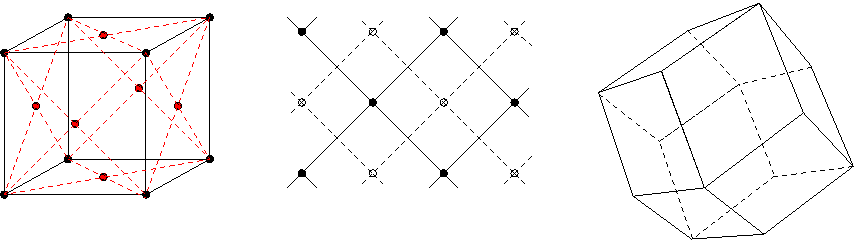
\includegraphics{./Schranken-figs/fcc}
  \caption{Links ein W\"urfel mit Vertices in allen Fl\"achen. In der Mitte sind die beiden durch Projektion entlang einer W\"urfelkante entstehenden Quadratgitter dargestellt. Rechts ist eine Skizze der WSZ des fcc-Gitters, ein rhombisches Dodekaeder, zu sehen.}
  \label{fig:fcc}
\end{figure}
Die Anzahlen der Zellen verschiedener Dimensionen lassen sich leicht bestimmen (siehe Appendix \ref{sec:appfcc}), und man erh\"alt f\"ur die Euler-Charakteristik
\begin{equation}
  \chi^{fcc-WSZ}_{12-18}(p)=p(1-p)(1-5p+3p^2+p^3+p^4).
\end{equation}
Neben den zw\"olf Zellen, die die WSZ an Fl\"achen ber\"uhrt, gibt es sechs weitere WSZ, die sie nur an einer Ecke ber\"uhrt. Somit gibt es insgesamt $18$ Zellen, mit denen eine WSZ einen nichtleeren Durchschnitt hat.\\
Alternativ zu den WSZ k\"onnen auch Prismen quadratischer Grundfl\"ache als Zellen benutzt werden. Das fcc-Gitter ist n\"amlich ein Stapel gegeneinander verschobener Quadratgitter (siehe Abb. \ref{fig:fcc}). Prismen mit quadratischer Grundfl\"ache sind Zellen, die die Zusammenhangsverh\"altnisse des Gitters widerspiegeln, denn sie haben mit den Zellen innerhalb der Ebene je eine Fl\"ache gemein, und obere und untere Fl\"achen \"uberlappen mit den Fu"s- bzw. Kopffl\"achen von vier Prismen aus den darunter bzw. dar\"uber liegenden Ebenen. An den senkrechten Kanten sto"sen die Prismen innerhalb einer Ebene mit den \"ubern\"achsten Nachbarn auf dem Quadratgitter zusammen. Eine Zelle kann also mit 16 Nachbarzellen einen nichtleeren Durchschnitt haben, statt 18 bei der WSZ. Die Euler-Charakteristik, die man mit den Prismen erh\"alt (siehe Appendix \ref{sec:appfcc}), ist
\begin{equation}
  \chi^{fcc-Qu}_{12-16}(p)=p(1-p)(1-5p+3p^2+2p^3).
\end{equation}
Zum Vergleich der beiden Euler-Charakteristiken sind sie links in Abbildung \ref{fig:fcc+bccplot} aufgetragen. Bis zur ersten Nullstelle, die in beiden F\"allen zw\"olf Nachbarn entspricht, unterscheiden sie sich kaum. F\"ur $p>0.3$ ist der Unterschied deutlich erkennbar.
\begin{figure}[htbp]
  \centering
  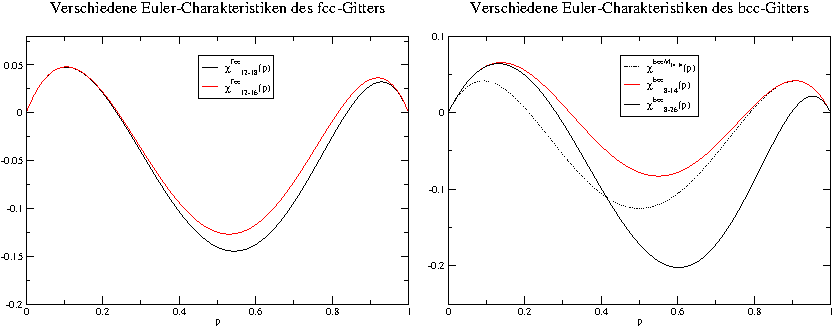
\includegraphics{./Schranken-figs/chiplot}
  \caption{Verschiedene Euler-Charakteristiken des fcc- (links) und bcc-Gitters (rechts).}
  \label{fig:fcc+bccplot}
\end{figure}

\subsection{bcc-Gitter}
Das bcc-Gitter (body centered cubic) entsteht, wenn in die Mitte jedes W\"urfels des sc-Gitter ein weiterer Vertex gesetzt wird (siehe Abb. \ref{fig:bcc}). Man erh\"alt das bcc-Gitter auch durch zwei \"uberlagerte, um eine halbe Raumdiagonale gegeneinander verschobene, sc-Gitter. Die n\"achsten Nachbarn eines Vertex des bcc-Gitter sind die acht Vertices auf den Ecken des umgebenden W\"urfels. Die WSZ des bcc-Gitters hat 14 Fl\"achen, davon acht Sechsecke, die den Gitterkanten entsprechen, und sechs Quadrate, die den Kanten der sc-Untergitter entsprechen. 
F\"ugt man die Kanten der sc-Gitter zum bcc-Gitter hinzu, erh\"alt man ein Gitter mit 14 Nachbarn. An jeder Kante der WSZ sto"sen nur drei und an jeder Ecke nur vier Zellen zusammen. D.h. es sto"sen keine Zellen zusammen, die nicht ohnehin eine gemeinsame Fl\"ache haben, und das Komplement hat die gleichen Zusammenhangsverh\"altnisse. Das bcc-Gitter mit 14 Nachbarn ist in dieser Hinsicht das dreidimensionale Analogon des zweidimensionalen Dreiecksgitters. Das 14er bcc-Gitter wurde in \cite{Likos:95} behandelt; die Euler-Charakteristik ist
\begin{equation}
  \chi_{14-14}^{bcc}(p)=p(1-p)(1-6p+6p^2).
\end{equation}
\begin{figure}[tbp]
  \centering
  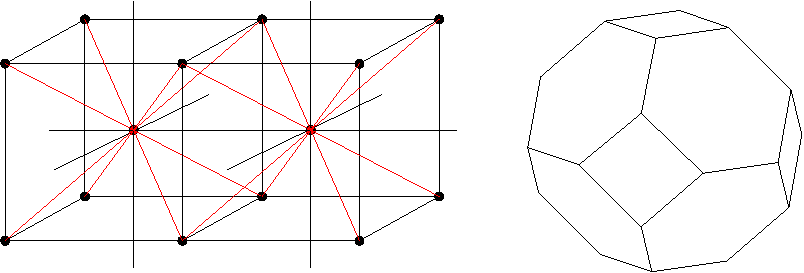
\includegraphics{./Schranken-figs/bcc}
  \caption{Bcc-Gitter: Links ist ein Ausschnitt des bcc-Gitter zu sehen. Die Gitterkanten sind mit roten Linien eingezeichnet; Kanten der sc-Untergitter sind schwarz gezeichnet. Rechts ist die Wigner-Seitz-Zelle (WSZ) des bcc-Gitter gezeigt.}
  \label{fig:bcc}
\end{figure}Um eine Euler-Charakteristik zu erhalten, die die Zusammenhangsverh\"altnisse des bcc-Gitter mit acht Nachbarn widerspiegelt, kann man entweder eine komplizierte Zelle (siehe Abbildung \ref{fig:bcc_nonconvex_app} und Kapitel \ref{sec:appbcc}) w\"ahlen, oder zwei WSZ nur dann als benachbart betrachten, wenn sie sich an einem Sechseck ber\"uhren. Zwei WSZ, die sich an einem Quadrat ber\"uhren, gelten dann nur als benachbart, wenn sie einen gemeinsamen besetzten Gitternachbarn haben (siehe Kapitel \ref{sec:mixedbcc}). Die Euler-Charakteristiken, die man mit den unterschiedlichen Methoden erh\"alt, unterscheiden sich im Wesentlichen in der Zahl der Zellen, mit denen ein abgeschlossene Zelle einen nichtleeren Durchschnitt hat. W\"ahrend eine nichtkonvexe Zelle mit 26 anderen Zellen einen nichtleeren Durchschnitt hat, sind es bei der WSZ nur 14. 
\begin{eqnarray}
  \chi_{8-26}^{bcc}(p)&=&p(1-p)(1-3p-3p^2+3p^3+3p^4)\\
  \chi_{8-14}^{bcc}(p)&=&p(1-p)(1-3p-3p^2+9p^3-3p^4).
\end{eqnarray}
Um die drei unterschiedlichen Euler-Charakteristiken zu vergleichen, sind im rechten Teil der Abb. \ref{fig:fcc+bccplot} aufgetragen. Wenn die Nachbarschaftszahlen $z$ bzw. $\bar{z}$ zweier Euler-Charak\-ter\-istiken \"ubereinstimmen, unterschieden sie f\"ur kleine bzw. gro"se $p$ kaum. So f\"allt $\chi_{8-26}^{bcc}(p)$ mit $\chi_{8-14}^{bcc}(p)$ f\"ur $p<0.3$ fast zusammen, w\"ahrend sie f\"ur gro"se $p$ stark unterschiedlich sind. F\"ur $p>0.7$ sind dagegen $\chi_{8-14}^{bcc}(p)$ und $\chi_{14-14}^{bcc}(p)$ sehr \"ahnlich. Im Bereich $p\approx \frac{1}{2}$ unterscheiden sich alle sehr stark, da die Bedingungen, unter denen ein ``Tunnel'' entstehen kann, unterschiedlich sind.

\subsection{Diamantgitter}
Das Diamantgitter ist ein fcc-Gitter mit zweiatomiger Basis, also kein Bravaisgitter. Wenn ein Vertex auf einem fcc-Vertex liegt, liegt der andere bei $(\frac{1}{4},\frac{1}{4},\frac{1}{4})$ auf der W\"urfeldiagonale des sc-Teilgitters. Ein Vertex hat vier n\"achste Nachbarn, die auf den Ecken eines Tetraeders um den Vertex liegen.
 
\subsubsection{Nichtkonvexe Zelle mit 4er-Nachbarschaft}
Um der Topologie des Diamantgitters mit seinen vier n\"achsten Nachbarn Rechnung zu tragen, ist eine Zelle n\"otig, die nur die Zellen der vier n\"achsten Nachbarn an einer Fl\"ache ber\"uhrt. Wie diese Zellen aussehen, und wie die Euler-Charakteristik berechnet wird, ist im Anhang \ref{sec:appdiamantnonconvex} beschreiben. Man erh\"alt f\"ur die Euler-Charakteristik 
\begin{equation}                     
        \chi^{Diamant}_{4-47}(p)=p(1-p)\left(\frac{p^{12}+p^{11}+p^{10}+p^9+p^8+p^7+p^6+p^5}{2}-p^4-p^3-p^2-p+1 \right).
\end{equation}
Diese Zellen ber\"uhren insgesamt 47 Zellen an Ecken, Kanten oder Fl\"achen.

\subsubsection{Konvexe Zellen mit 4er-Nachbarschaft}
Nun betrachten wir eine WSZ des fcc-Gitters und halbieren sie senkrecht zur Basisachse (siehe Abb. \ref{fig:fcc_half}). Die gemeinsame Schnittfl\"ache und die drei Rhomben auf der gegen\"uberliegenden Seite geh\"oren zu einer Gitterkante des Diamantgitters. Alle anderen Seiten entsprechen keinen Gitternachbarschaften, und zwei Zellen sollen \"uber diese Seiten nur zusammenh\"angen, wenn sie einen gemeinsamen n\"achsten Nachbarn haben. Analog zur Prozedur aus Kapitel \ref{sec:mixedbcc} kann so eine Euler-Charakteristik des Diamantgitters berechnet werden. Die im Anhang \ref{sec:appdiamantconvex} beschriebene Rechnung liefert: 
\begin{equation}
  \chi^{Diamant}_{4-19}(p)=p(1-p)(p^8+p^7+p^6+p^5-4p^4+2p^3-p^2-p+1).
\end{equation}
Eine halbierte WSZ kann mit 19 anderen Zellen einen nichtleeren Durchschnitt haben. \\

In Abbildung \ref{fig:diamantplot} sind die beiden Euler-Charakteristiken des Diamantgitters aufgetragen. Beide Euler-Charakteristiken sind f\"ur kleine $p$ \"ahnlich. Dadurch, dass die Zellen zur Berechnung von $\chi^{Diamant}_{4-47}(q)$ sehr viele andere Zellen an Ecken oder Kanten ber\"uhren, entstehen Tunnel sehr viel einfacher als bei Verwendung der konvexen Zellen, und $\chi^{Diamant}_{4-47}(p)$ ist f\"ur $p\approx0.5$ kleiner als $\chi^{Diamant}_{4-19}(p)$.
\begin{figure}[tbp]
  \centering
  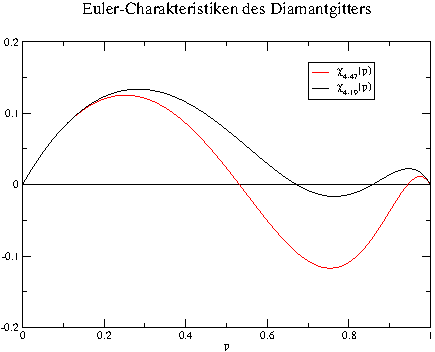
\includegraphics{./Schranken-figs/chidiamant}
  \caption{Verschiedene Euler-Charakteristiken des Diamantgitters.  }
  \label{fig:diamantplot}
\end{figure}

\section{Euler-Charakteristik und Perkolation in drei Dimensionen}
Jeder Euler-Charakteristik der dreidimensionalen Gitter  haben wir ein Paar von Zahlen $(z,\bar{z})$ zugeordnet. Die erste Zahl $z$ ist die Koordinationszahl des Gitters. Die zweite Zahl $\bar{z}$ ist die Zahl der Zellen, mit denen eine abgeschlossene Zelle einen nichtleeren Durchschnitt haben kann. Wenn man auf dem Gitter alle Vertices verbindet, deren Zellen einen nichtleeren Durchschnitt haben, erh\"alt man ein Gitter mit der Topologie der unbesetzten Bereiche. Dieses Gitter hat die Koordinationszahl $\bar{z}$. Die Gitter mit Zusammenhangsverh\"altnissen der unbesetzten Bereiche entsprechen den matching-Gittern in zwei Dimensionen. Da die Wahl der Zellen aber nicht eindeutig ist, sind auch die ``matching''-Gitter in drei Dimensionen nicht eindeutig. 
\\Jede der berechneten Euler-Charakteristiken dreidimensionaler Gitter hat zwei Nullstellen zwischen null und eins. Die kleinere von beiden markiert den \"Ubergang von isolierten Clustern zu vernetzten Strukturen, in denen Tunnel \"uberwiegen. Sie wird der Perkolationsschwelle des Gitter mit $z$ Nachbarn zugeordnet.  Die zweite Nullstelle markiert den \"Ubergang vernetzter Strukturen zu isolierten Einschl\"ussen und wird daher der Perkolationsschwelle der unbesetzten Bereiche zugeordnet. Wenn explizit die Euler-Charakteristik $\bar{\chi}(q)$ der unbesetzten Vertices, d.h. des ``matching''-Gitters, betrachtet wird, sind die Rollen von $z$ und $\bar{z}$ vertauscht und $\bar{\chi}_{\bar{z},z}(q)=\chi_{z,\bar{z}}(p)$. 
\\Auch in drei Dimensionen best\"atigt sich die Vermutung, dass die Nullstelle der Euler-Charakteristik in der Regel eine obere Schranke an die Perkolationsschwelle ist. Das gilt sowohl f\"ur die Perkolation auf den untersuchten Gittern, als auch f\"ur die Perkolation auf den ``matching''-Gittern, sofern deren Perkolationsschwellen bekannt sind. Nur die Euler-Charakteristik des sc-Gitters mit 18 Nachbarn f\"allt aus der Reihe, was wohl daran liegt, dass sowohl das Gitter selbst, als auch das ``matching''-Gitter sehr hohe Koordinationszahlen haben. In Abbildung \ref{fig:3dallplots} sind die Perkolationsschwellen $p_c$ und die Nullstellen $p_0$ der Euler-Charakteristik f\"ur alle behandelten Gitter aufgetragen. Die numerischen Werte der Nullstellen und Perkolationsschwellen sind in den Tabellen \ref{tab:stacked} und \ref{tab:3dall} zusammengefasst. Tr\"agt man die Nullstellen der Euler-Charakteristiken gegen $z$ auf (Plot in Abb. \ref{fig:pooverz}), beobachtet man in etwa $p_0\sim \frac{1}{z}$.


 
\begin{table}
  \centering
  \begin{tabular} {|l|r|r|r||r|}
\hline
Name & $z$&$\bar{z}$ & $p_0$ & $p_c$ \\ \hline
Diamant (nicht konvex)&$4$&$47$&$0.5318$ & $0.4286(4)$ \\ \hline
Diamant (konvex)&$4$&$19$&$0.6722$ & $0.4286(4)$ \\ \hline
sc (WSZ)&$6$&$26$&$0.3940$&$0.3114(4)$\\ \hline
bcc (nicht konvex)& $8$&$26$ &$0.2825$&$0.2458(4)$ \\ \hline
bcc (konvex)&$8$&$14$&$0.3185$&$0.2458(4)$ \\ \hline
fcc (WSZ)&$12$&$18$&$0.2370$&$0.1994(2)$ \\ \hline
fcc (Prisma)&$12$&$16$&$0.2401$& $0.1994(2)$\\ \hline
bcc (WSZ)&$14$&$14$&$0.2113$ &$0.175$\\ \hline 
sc (WSZ)&$18$&$26$&$0.1344$ & $0.137$\\ \hline \hline
bcc (WSZ)&$14$&$8$&$0.2185$&$0.175$ \\ \hline 
fcc (Prisma)&$16$&$12$&$0.1851$& -- \\ \hline
fcc (WSZ)&$18$&$12$&$0.1616$&  $0.136$\\ \hline
Diamant (konvex)&$19$&$4$&$0.1425$ & -- \\ \hline
sc (WSZ)&$26$&$6$&$0.1139$& $0.097$\\ \hline
bcc (nicht konvex)&$26$&$8$&$0.1033$&$0.095$\\ \hline
Diamant (nicht konvex)& $47$&$4$&$0.0561$ & --  \\\hline  

\end{tabular}
\caption{Dreidimensionale Gitter: Nullstellen $p_0$ der verschiedenen Euler-Charakteristiken im Vergleich zu den Perkolationsschwellen $p_c$. Die zur Berechnung der Euler-Charakteristik verwendeten Zellen und die resultierenden Koordinationszahlen besetzter und unbesetzter Zellen sind jeweils angegeben. Eintr\"age unterhalb des Doppelstrichs geh\"oren zu ``matching''-Gittern. Vierstellige Perkolationsschwellen mit Fehlergrenzen stammen aus \cite{Marck:97}, die \"ubrigen aus \cite{Essam:72}. Letztere sind vermutlich sehr ungenau. }
\label{tab:3dall}
\end{table}

\begin{figure}[htbp]
  \centering
  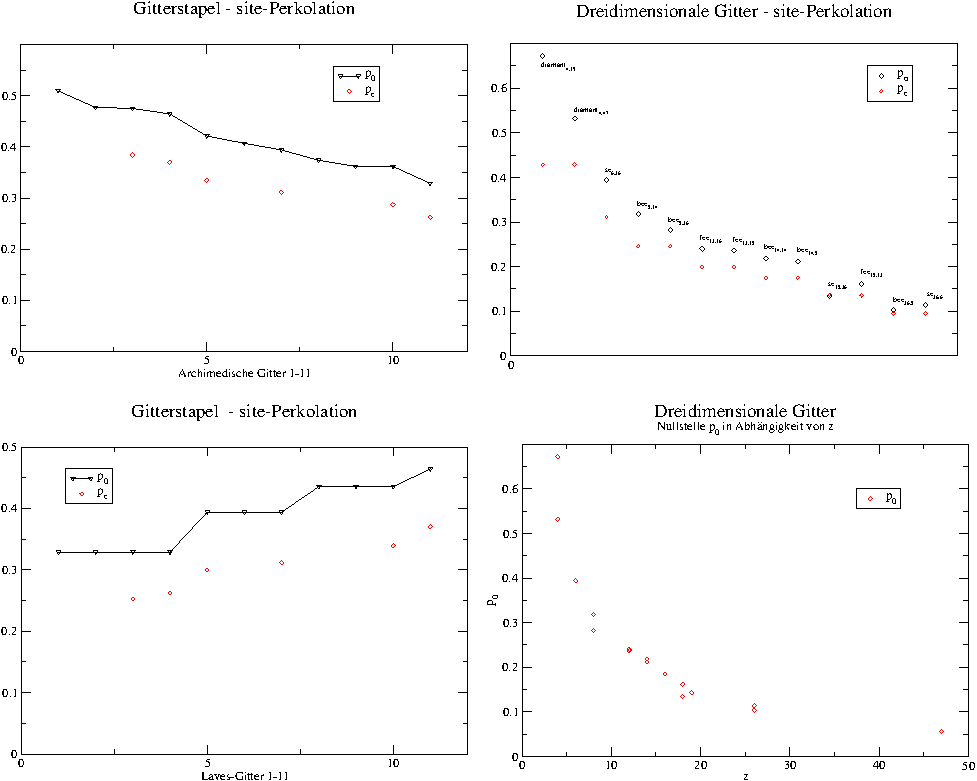
\includegraphics[height=22cm]{./Schranken-figs/3d}
  \caption{Ergebnisse in drei Dimensionen: Die oberen beiden Grafiken zeigen die Nullstellen $p_0$ der Euler-Charakteristik und Perkolationsschwellen $p_c$ f\"ur die Gitterstapel der archimedischen Gitter (oben) und der Laves-Gitter (Mitte). Der unterste Plot enth\"alt $p_0$ und $p_c$ der \"ubrigen untersuchten Gitter.}
  \label{fig:3dallplots}
\end{figure}
\begin{figure}[htbp]
  \centering
  \includegraphics[height=6cm]{./Schranken-figs/pooverz_fig}
  \caption{Variation der Nullstelle $p_0$ der Euler-Charakteristik mit der Zahl der Nachbarn $z$ eines Vertex. Es gilt in etwa $p_0\sim 1/z$. Siehe auch Tabelle \ref{tab:3dall}. }
 \label{fig:pooverz}
\end{figure}

\section{Bond-site-Perkolation}
In Kapitel \ref{sec:mixed} wurde eine Methode vorgestellt, mit der die mittlere Euler-Charakteristik von Konfigurationen, wie sie bei bond-site-Perkolation entstehen, berechnet werden kann. Hier wird die Nullstelle der so berechneten Euler-Charakteristiken mit den bond-site-Perkolationsschwellen der Gitter verglichen.
\\Der kritische Ort eines gemischten bond-site-Perkolationsproblem mit Besetzungswahrscheinlichkeiten $p_s$ und $p_b$ f\"ur Vertices und Kanten ist eine Kurve $[p_s^*(t),p_b^*(t)]_c$ in der $(p_s,p_b)$-Ebene mit einem geeigneten Parameter $t$. Die Kurve l\"asst sich in der Regel sowohl durch $p_b^*$ als auch durch $p_s^*$ parametrisieren. In Ref. \cite{Yanuka:90} wird folgende empirische Beziehung f\"ur die bond-site-Perkolationsschwellen $[p_s^*(t),p_b^*(t)]$ vorgestellt:
\begin{equation}
\label{eq:bondsitepc}
  \frac{\ln p^*_s}{\ln p^*_b}+\frac{\ln p_c^{site}}{\ln p_c^{bond}}=1.
\end{equation}
Die Parameter $p_c^{site}$ und $p_c^{bond}$ sind die Perkolationsschwellen der reinen site- bzw. bond-Perkolation. Die durch Gl. \ref{eq:bondsitepc} gegebene Kurve stimmt bis auf wenige Promille mit den Simulationsergebnissen f\"ur bond-site-Perkolation \"uberein. Die G\"ultigkeit von Gl. \ref{eq:bondsitepc} wurde in Ref. \cite{Tarasevich:99} weiter untersucht, und es wurde sehr gute \"Ubereinstimmung f\"ur zweidimensionale Gitter und Abweichungen von maximal einem Prozent f\"ur h\"oher dimensionale Gitter festgestellt. Die Gl. \ref{eq:bondsitepc} l\"asst sich nach $p^*_b$ oder $p^*_s$ aufl\"osen und man erh\"alt f\"ur die kritische site-Besetzungswahrscheinlichkeit $p^*_s$ bei gegebenem $p_b^*\in [p_c^{bond},1]$
\begin{equation}
\label{eq:bondsitefit}
p^*_s\left(p^*_b\right)=p_c^{site}\left[p^*_b\right]^{-\frac{\ln p_c^{site}}{\ln p_c^{bond}}}.
\end{equation}
Die Genauigkeit dieser empirischen Formel reicht f\"ur den Vergleich mit der Nullstelle der Euler-Charakteristik aus, und statt Simulationsdaten wird f\"ur $[p^*_s,p^*_b]$ die Gleichung \ref{eq:bondsitefit} benutzt.\\
Die mittlere Euler-Charakteristik pro Vertex $\chi(p_s,p_b)$ ist ein Polynom in $p_s$ und $p_b$. $\chi(p_s,p_b)$ hat einige allgemeine Eigenschaften: Ist $p_b=0$, so besteht die Anordnung aus isolierten, abgeschlossenen Zellen und $\chi(p_s,0)=p_s$. F\"ur $p_s=0$ sind \"uberhaupt keine Zellen vorhanden und $\chi(0,p_b)=0$. Der Fall $p_b=1$ entspricht der \"ublichen site-Perkolation und $\chi(p_s,1)=\chi^{site}(p_s)$. Der letzte Extremfall mit $p_s=1$ entspricht einer speziellen Geometrie der bond-Perkolation, bei der, ausgehend von isolierten Zellen, nach und nach Verbindungen durch Verschmelzen von $(d-1)$-Nachbarschaften hinzugef\"ugt werden. $\chi(1,p_b)$ unterscheidet sich von der Euler-Charakteristik, die durch \"Ubergang zum \"Uberdeckungsgitter erhalten wurde.
\begin{figure}[tbp]
  \centering
  \includegraphics{./Schranken-figs/bond-site2d}
  \caption{$p_s^*(p_b)$ und $p_{s0}(p_b)$ ist links f\"ur das Dreiecks- und rechts f\"ur das Quadratgitter aufgetragen. F\"ur $p_s^*(p_b)$ ist die in \cite{Yanuka:90} vorgeschlagene Formel benutzt worden.}
  \label{fig:bond-site2d}
\end{figure}
\\In zwei Dimensionen wurde $\chi(p_s,p_b)$ f\"ur das Quadrat- (siehe Kap. \ref{sec:bondsitesq}) und das Dreiecksgitter (siehe Anhang \ref{sec:appbond-site}) ausgerechnet. Die Euler-Charakteristik der bond-site-Perkolation auf dem Dreiecksgitter ist
\begin{equation}
\chi^{tr}(p_s,p_b)=p_s-3p_bp_s^2+2p_b^3p_s^3.
\end{equation}
F\"ur das Quadratgitter erh\"alt man
\begin{equation}
\chi^{sq}(p_s,p_b)=p_s-2p_bp_s^2+p_b^4p_s^4.
\end{equation}
Aus der Gleichung $\chi(p_s,p_b)=0$ erh\"alt man eine Kurve $p_{s_0}(p_b)$ und kann diese mit $p^*_s\left(p^*_b\right)$ vergleichen. In beiden F\"allen hat $p_{s_0}(p_b)$ in etwa die gleiche Form wie die kritische Kurve, und beide Kurven liegen dicht zusammen (siehe Abb. \ref{fig:bond-site3d}). Beim Quadratgitter liegt die Nullstelle immer jenseits der Perkolationsschwelle, im Fall des Dreiecksgitters schneiden sich beide Kurven.
\\In drei Dimensionen wurde $\chi(p_s,p_b)$ f\"ur das fcc-Gitter (siehe Anhang \ref{sec:appbond-site}) und das sc-Gitter (siehe Kap. \ref{sec:bondsitesc}) ausgerechnet. 
\begin{equation}
 \chi^{fcc}(p_s,p_b)=p_s-6p_s^2p_b+8p_s^3p_b^3-2p_s^4p_b^6-p_s^6p_b^{12}.
\end{equation}
\begin{equation}
\chi^{sc}(p_s,p_b)= p_s-3p_s^2p_b+3p_s^4p_b^4-p_s^8p_b^{12}.
\end{equation}
Beim fcc- und sc-Gitter liegt $p_{s_0}(p_b)$ immer jenseits von $p_s^*(p_b^*)$, und beide Kurven haben fast identische Form (siehe Abb. \ref{fig:bond-site3d}).
\\

Auch bei bond-site-Perkolation best\"atigt sich die Beobachtung, dass die Nullstelle der Euler-Charakteristik in der N\"ahe der Perkolationsschwelle liegt. Beim zweidimensionalen Quadratgitter und bei den dreidimensionalen Gittern liegt die Nullstelle jenseits der Perkolationsschwelle, analog zu $p_c<p_0$ bei der reinen site-Perkolation. Neben den in Abschnitt \ref{sec:chibond} f\"ur bond-Perkolation auf archimedischen Gittern berechneten Euler-Charakteristiken, kann aus $\chi(p_s=1,p_b)$ eine weitere Euler-Charakteristik f\"ur bond-Perkolation erhalten werden. Die Nullstellen dieser Euler-Charakteristik liegt in allen F\"allen, anders als bei den Euler-Charakteristiken der \"Uberdeckungsgittern, \"uber der Perkolationsschwelle.

\begin{figure}[htbp]
  \centering
  \includegraphics[height=20cm]{./Schranken-figs/bond-site3d}
  \caption{Die Kurven $p_s^*(p_b)$ und $p_{s_0}(p_b)$ haben sowohl f\"ur das fcc-, als auch f\"ur das sc-Gitter fast identische Form. Die d\"unnen Linien sind die H\"ohenlinien der $\chi(p_s,p_b)$-''Landschaft''. F\"ur $p_s^*(p_b)$ ist die in Ref. \cite{Yanuka:90} vorgeschlagene Formel benutzt worden.}
  \label{fig:bond-site3d}
\end{figure}
  %25.9.2003

\chapter{Gegenbeispiele}
\label{sec:grenzen}

Die in der Einleitung vorgestellte Beziehung zwischen der Perkolationsschwelle und der Nullstelle der mittleren Euler-Charakteristik hat sich in Kapitel \ref{sec:schranken} im Wesentlichen best\"atigt. Auch die Vermutung, dass die Perkolationsschwelle in zwei Dimensionen immer zwischen Wendepunkt und Nullstelle der Euler-Charakteristik liegt, scheint bei einer gro"sen Klasse von Gittern zu stimmen. Es gibt aber auch Gitter, bei denen diese Beziehungen nicht gelten. Im Folgenden sollen diese Gitter vorgestellt und ihre gemeinsamen Eigenschaften identifiziert werden.

\section{site-Perkolation}
Steven van der Marck hat das Quadrat- und das Kagom\'e-Gitter auf verschiedene Arten modifiziert und f\"ur die so erhaltenen zehn neuen Gitter die Perkolationsschwellen numerisch bestimmt. Die Gitter, die van der Marck betrachtet, sind in Abbildung \ref{fig:vandermarck} dargestellt.
\begin{figure}[htbp]
  \centering
  \includegraphics{./Grenzen-Figs/vandermarck}
  \caption{Modifizierte Quadrat- und Kagom\'e-Gitter aus \cite{Marck:03}. }
  \label{fig:vandermarck}
\end{figure}
Die Gitter haben entweder nur zwei Vertextypen, oder bestehen nur aus viereckigen Plaketten. Die Euler-Charakteristiken der Gitter, die nur zwei Vertextypen haben, k\"onnen mit Gleichung (\ref{eq:2-uniform}) ausgerechnet werden. Die Euler-Charakteristiken der \"ubrigen Gitter sind gleich der des Quadratgitters. Die Bezeichungen der Gitter sind in Abbildung \ref{fig:vandermarck} und ihre Vertexkonfigurationen in Tabelle \ref{tab:marckirreg} zu finden. In der Tabelle sind auch die Nullstellen und Wendepunkte der Euler-Charakteristiken und die Perkolationsschwellen der Gitter angegeben.
\begin{table}
\centering
\begin{tabular}{|l|l|r|r||r|}
\hline
Gittername & Vertexkonfiguration & $p_0$ & $p_0^{(2)}$& $p_c$   \\ \hline
\hline

embedded Kagom\'e & $\frac{2}{3}\left[3,3,3,12\right]+\frac{1}{3}\left[3,12,3,12\right]$&0.7580 & $0.6863$&$0.7406(3)$\\ \hline

embedded square & $\frac{2}{3}\left[3,4,3,8\right]+\frac{1}{3}\left[3,8,3,8\right]$&$0.6965$ & $0.6384$&$0.6766(3)$\\ \hline

tic-tac-toe&$ \frac{1}{3}\left[3,3,3,3\right]+\frac{2}{3}\left[3,3,4,3,3,4\right]$&$0.5414$ & $0.5275$&$0.5448(3)$\\ \hline

filled Kagom\'e & $\frac{2}{5}\left[3,3,3\right]+\frac{3}{5}\left[3,3,6,3,3,6\right]$  & $0.6093$ & $0.5754$&$0.6527\dots $ \\ \hline

star Kagom\'e&$ \frac{2}{3}\left[3,6,3,6\right]+\frac{1}{3}\left[3,6,3,6\right]$&$0.6756$ & $0.6231$&$0.7406(2)$ \\ \hline

embedded Kagom\'e dual & wie Quadratgitter &$0.6180$ & $0.5774$&$0.5510(3)$ \\ \hline

embedded square dual &wie Quadratgitter &$0.6180$ & $0.5774$&$0.5770(3)$ \\ \hline

tic-tac-toe dual & $\frac{1}{5}\left[6,6,6,6\right]+\frac{4}{5}\left[4,6,6\right]$&$0.7200$ & $0.6527$&$0.6779(3)$ \\ \hline

filled Kagom\'e dual &$\frac{1}{7}\left[6,6,6,6,6,6\right]+\frac{6}{7}\left[3,6,6\right]$&$0.7156$ & $0.6512$&$0.6599(2)$  \\ \hline

star Kagom\'e dual & wie Quadratgitter&$0.6180$& $0.5774$&$0.5515(2)$  \\ \hline

\end{tabular}
\caption{Die Perkolationsschwelle $p_c$ modifizierter archimedischer Gitter liegt h\"aufig nicht zwischen der Nullstelle $p_0$ und dem Wendepunkt $p_0^{(2)}$ der Euler-Charakteristik. Die Namen der Gitter und die Perkolationsschwellen sind aus \cite{Marck:03} \"ubernommen. ``wie Quadratgitter'' soll bedeuten, dass die Euler-Charakteristik gleich der des Quadratgitters ist. Diese Gitter haben mehr als zwei unterschiedliche Vertextypen, aber nur viereckige Plaketten.}
\label{tab:marckirreg}
\end{table}
Bei vielen dieser Gitter liegt $p_c$ nicht zwischen $p_0$ und $p_0^{(2)}$. Die gr\"o"sten Abweichungen von $p_c$ nach oben sind beim \textit{filled Kagom\'e}- und \textit{star Kagom\'e}-Gitter zu finden. Beim \textit{filled Kagom\'e}-Gitter tragen die Vertices in den Dreiecken des Kagom\'e-Gitters nicht zur Konnektivit\"at bei, denn zwei Vertices auf den Ecken eines Dreiecks sind miteinander verbunden, unabh\"angig davon, ob der Vertex im Dreieck besetzt oder leer ist. Das Gitter perkoliert genau dann, wenn das Kagom\'e-Untergitter perkoliert; $p_c$ ist daher gleich $p_c^{Kagome}=1-2\sin(\pi/18)$. Die Euler-Charakteristiken der beiden Gitter sind aber verschieden. Insbesondere ist die Nullstelle erheblich kleiner, da unbesetzte Vertices in den Dreiecken zus\"atzliche L\"ocher erzeugen k\"onnen.\\
Beim \textit{embedded Kagom\'e dual-} und beim \textit{star Kagom\'e dual}-Gitter ist $p_c$ kleiner als $p_0^{(2)}$. Alle Plaketten dieser Gitter sind Vierecke, und die Euler-Charakteristik ist daher die gleiche wie beim Quadratgitter. Es gibt aber einige Vertices mit hoher und andere mit kleiner Koordinationszahl. Diese Inhomogenit\"at f\"uhrt offensichtlich zu einer Absenkung von $p_c$. Dieser Effekt ist beim \textit{embedded square dual}-Gitter nicht so stark ausgepr\"agt. $p_c$ ist auch dort niedriger als beim Quadratgitter, aber nicht so niedrig wie bei den obigen Gittern und in etwa gleich $p_0^{(2)}$. 

\subsection*{Cluster der Gr\"o"se 1 auf dem \textit{filled Kagom\'e}-Gitter}
Um die Absenkung der Nullstelle der Euler-Charakteristik relativ zur Perkolationsschwelle des \textit{filled Kagom\'e}-Gitters zu untersuchen, bestimmen wir die Beitr\"age der Cluster und L\"ocher der Gr\"o"se 1 zur Euler-Charakteristik. Ein Cluster der Gr\"o"se 1 entsteht, wenn ein Vertex besetzt und alle seine Nachbarn unbesetzt sind. 
\\Die Vertices innerhalb der Dreiecke haben drei Nachbarn und stellen $\frac{2}{5}$ der Vertices. Die \"ubrigen Vertices haben sechs Nachbarn. Die erwartete Zahl der Cluster der Gr\"o"se 1 ist also
\begin{equation}
  n_1(p)=\frac{2pq^3+3pq^6}{5},
\end{equation}
wobei $q=1-p$ ist. Auf dem matching-Gitter haben die Vertices in den Dreiecken die gleiche Nachbarzahl, w\"ahrend die \"ubrigen Vertices zw\"olf Nachbarn haben. F\"ur erwartete Zahl der Cluster der Gr\"o"se 1 auf dem matching-Gitter erh\"alt man also
\begin{equation}
  n_1^*(p)=\frac{2pq^3+3pq^{12}}{5}.
\end{equation}
Im Abschnitt \ref{sec:scaling} wurde die Euler-Charakteristik $\chi_{s_0}(p)$, eingeschr\"ankt auf Cluster und L\"ocher der Gr\"o"se $s\geq s_0$, betrachtet. Zieht man $n_1(p)-n_1^*(q)$ von der Euler-Charakteristik $\chi^{f-Kagome}(p)$ des \textit{filled Kagom\'e}-Gitters ab, erh\"alt man $\chi^{f-Kagome}_2(p)$. Die Nullstelle und der Wendepunkt von $\chi^{f-Kagome}_2(p)$ liegen bei $p_0=0.6804$ und $p_0^{(2)}=0.6220$. Das blo"se Abziehen der Beitr\"age kleinster Cluster ``repariert'' also die Abweichung von $p_0>p_c>p_0^{(2)}$.

\section{bond-Perkolation}
Die Perkolationsschwelle des archimedischen Gitters mit Vertexkonfiguration $(3,4,3,6)$ liegt oberhalb der Nullstelle der Euler-Charakteristik, obwohl $p_c>\frac{1}{2}$ ist. Die Abweichung ist aber nur gering und $p_c$ nur numerisch bekannt.\\
Ein Gegenbeispiel mit exakt bekannter Perkolationsschwelle erh\"alt man, indem jede Gitterkante des Sechseckgitters durch den Graphen, der in Abb. \ref{fig:hexbond} angegeben ist, ersetzt wird.
\begin{figure}[htbp]
  \centering
  \includegraphics{./Grenzen-Figs/figure}
  \caption{Graph, durch den die Gitterkanten des Sechseckgitters ersetzt werden.}
  \label{fig:hexbond}
\end{figure}
Die bond-Perkolationsschwelle des Sechseckgitters ist exakt bekannt. Die Perkolationsschwelle des modifizierten Gitters ergibt sich aus der Bedingung, dass die Wahrscheinlichkeit, dass der Graph aus Abb. \ref{fig:hexbond}, durchg\"angig ist, gleich der bond-Perkolationsschwelle des Sechseckgitters ist.\\
Diese Wahrscheinlichkeit kann durch Abz\"ahlen aller Konfigurationen ausgerechnet werden. Die beiden Kanten an den Enden des Graphens m\"ussen offen sein, daher ein Faktor $p^2$. Der Graph ist sicherlich durchg\"angig, wenn h\"ochstens eine der mittleren Kanten geschlossen ist, daher ein Beitrag $p^5+5p^4q$. Es gibt zwei M\"oglichkeiten, von den f\"unf mittleren Kanten zwei zu schlie"sen, so dass keine Verbindung von links nach rechts existiert. Es bleiben acht offene Konfigurationen mit zwei geschlossenen Kanten, und man erh\"alt einen Beitrag $8p^3q^2$. Sind nur zwei der f\"unf Kanten offen, gibt es zwei M\"oglichkeiten f\"ur eine offene Verbindung und daher einen Beitrag $2p^2q^3$. Ist nur eine der f\"unf Kanten offen, ist die Verbindung unterbrochen. $p_c$ ist also L\"osung der Gleichung
\begin{equation}
  1-2\sin\left(\frac{\pi}{18}\right) =p^2(p^5+5p^4q+8p^3q^2+2p^2q^3).
\end{equation}
Die einzige L\"osung zwischen null und eins ist $p_c=0.833702\ldots$.\\
Die Euler-Charakteristik des \"Uberdeckungsgitters l\"asst sich mit Gleichung (\ref{eq:matchingpoly}) ausrechnen, und man erh\"alt
\begin{equation}
  \chi(p)=-q+2(1-p^2)-\frac{20}{21}(1-p^3)-\frac{1}{21}(1-p^{24}).
\end{equation}
$\chi(p)$ hat eine Nullstelle bei $p_0=0.82208$; $p_0$ ist also kleiner als $p_c$. Durch das explizite Einf\"uhren einer Substruktur wird auch hier die Euler-Charakteristik abgesenkt, und die Nullstelle ``rutscht'' unter $p_c$.

\section{Eine Folge von Gittern mit $p_c=\frac{1}{2}$ und variierender Euler-Charakteristik}
Ausgehend von einem Dreiecksgitter, wird eine Folge von Gittern $\{\mathcal{G}_n\}$ konstruiert, deren mittlere Euler Charakteristik f\"ur $n=0$ die des Dreiecksgitter ist, und f\"ur $n \rightarrow \infty$ gegen die des Quadratgitters konvergiert. F\"ur alle $n$ ist die site-Perkolationsschwelle $p_c=\frac{1}{2}$.\\
Die Gitter entstehen, wenn man in jedes Dreieck des Dreiecksgitter ein weiteres Dreieck setzt, und dessen Ecken mit den Ecken des \"au"seren Dreiecks verbindet. Die Perkolationsschwelle des Gitters \"andert sich dadurch nicht, da die Vertices an den Ecken des \"au"seren Dreiecks ohnehin miteinander verbunden sind. In das innere Dreieck wird eine Pyramide aus Quadraten eingeschrieben (siehe Abb. \ref{fig:seqgitter}).
\begin{figure}[tbp]
  \centering
  \includegraphics{./Grenzen-Figs/seqgitter}
  \caption{Links: In die Dreiecke eines Dreiecksgitter wird eine Substruktur eingef\"uhrt. Diese Substrukturen sind f\"ur $n=0$, $n=1$ und $n=5$ gezeigt. Rechts ist ein gr\"o"serer Ausschnitt des Gitters mit $n=3$ zu sehen.}
  \label{fig:seqgitter}
\end{figure}
\\Die F\"alle $n=1$ und $n=0$ m\"ussen gesondert betrachtet werden (siehe Abb. \ref{fig:seqgitter}). F\"ur $n=0$ entartet das eingeschriebene Dreieck zu einem Vertex, f\"ur $n=1$ ist das innere Dreieck leer.\\
Die Euler-Charakteristik l\"asst sich mit den bekannten Methoden ausrechnen, und man erh\"alt eine Folge von Nullstellen $p_{n_0}$. Die Folge der Nullstellen hat bei $n=6$ ein Maximum und konvergiert dann langsam gegen $p_0=0.618$ des Quadratgitters (siehe Abb. \ref{fig:sequenze}). 
\begin{figure}[tbp]
  \centering
  \includegraphics{./Grenzen-Figs/sequenze1}
  \caption{Die Nullstellen $p_{n_0}$ der mittleren Euler-Charakteristik der Gitter $\mathcal{G}_n$. Die beiden horizontalen Linien markieren die Perkolationsschwelle der Gitter $p_c=\frac{1}{2}$ und die Nullstelle der Euler-Charakteristik des Quadratgitters $p_0^{sq}=0.618$.}
  \label{fig:sequenze}
\end{figure}\\

Der Zusammenhang zwischen den Nullstellen der Euler-Charakteristik und Perkolationschwellen kann offensichtlich durch Substrukturen zerst\"ort werden. Die Perkolationsschwelle und die Nullstelle der Euler-Charakteristik reagieren unterschiedlich auf Substruktur. W\"ahrend die mittlere Euler-Charakteristik nur durch lokale Beitr\"age erzeugt wird, h\"angen Perkolationsschwellen vor allem von globalen Eigenschaften des Gitters ab. Substrukturen sind f\"ur Perkolation irrelevant und k\"onnen renormiert werden. Im Abschnitt \ref{sec:scaling} wurde schon erw\"ahnt, dass $p_c<p_0$ dann gelten sollte, wenn sich das Skalenverhalten gro"ser Cluster qualitiv auf kleine Cluster fortsetzt. Bei Gittern mit Substruktur ist aber gerade das nicht der Fall.


\section[Gegenbeispiele -- Kontinuumsperkolation]{Kontinuumsperkolation von Kreisringen oder Kugeln verschiedener Radii}
Auch bei Kontinuumsperkolation kann man F\"alle finden, in denen aus der mittleren Euler-Charakteristik keine sinnvollen Aussagen \"uber Perkolationsschwellen gewonnen werden k\"onnen. Das einfachste Beispiel ist die Perkolation von Kreisringen in zwei Dimensionen. Die Euler-Charakteristik einer Vereinigung von Kreisringen ist immer negativ und kann daher keine Information \"uber $p_c$ liefern \cite{Mecke:94}. Ein anderes Beispiel ist Kontinuumsperkolation von Kugeln zwei verschiedener Radii. Hat ein kleiner Anteil der Kugeln einen gro"sen Radius und die \"ubrigen Kugeln einen sehr kleinen Radius, werden die gro"sen Kugeln bei gen\"ugend hoher Punktdichte perkolieren. Durch die vielen isolierten kleinen Kugeln ist die Euler-Charakteristik aber positiv und bei geeigneter Wahl des Gr\"o"senverh\"altnisses der Kugeln kann die Nullstelle der Euler-Charakteristik zu beliebig hohen Punktdichten verschoben werden, obwohl die gro"sen Kugeln perkolieren. Untersuchungen zur Abh\"angigkeit der Perkolationsschwelle und Euler-Charakteristik von Polydispersit\"at sind in Ref. \cite{Mecke:02} zu finden.
  %25.09.03

\chapter{Zusammenfassung und Ausblick}
\label{sec:zusammenfassung}


\section*{Euler-Charakteristik und Perkolationsschwellen in zwei Dimensionen}
In der Einleitung wurde die Beobachtung vorgestellt, dass die site-Perkolationsschwelle $p_c$ jedes archimedischen Gitters immer zwischen der Nullstelle $p_0$ und dem Wendepunkt $p_0^{(2)}$ der mittleren Euler-Charakteristik liegt. Genauer gilt f\"ur alle archimedischen Gitter $p_0^{(2)}<p_c<p_0$, und das arithmetische Mittel von $p_0$ und $p_0^{(2)}$ liefert eine exzellente Approximation von $p_c$. Dieser Befund war der Ausgangspunkt f\"ur weitere Untersuchungen in zwei Dimensionen. Dazu wurde die Euler-Charakteristik einer Vielzahl zweidimensionaler Gitter berechnet, und mit den, zumeist numerisch bestimmten, Perkolationsschwellen verglichen. Dar\"uberhinaus liefert das Skalenverhalten der Cluster bei $p_c$ Argumente f\"ur die G\"ultigkeit der Beobachtung.
\begin{itemize}
\item Die Perkolationsschwellen aller ``self-matching'' Gitter fallen mit der Nullstelle der Euler-Charakteristik zusammen. Auch f\"ur die eindimensionale Kette und das Bethe-Gitter gilt $p_0=p_c$.
\item F\"ur site-Perkolation auf Laves-Gittern, auf 2-uniformen Gittern und auf einigen irregul\"aren Gittern gilt $p_0^{(2)}\leq p_c \leq p_0$. Die site-Perkolationsschwellen der 2-uniformen Gitter waren nicht bekannt und wurden numerisch bestimmt. 
\item Die Euler-Charakteristiken der \"Uberdeckungsgitter wurden f\"ur alle archimedischen Gitter und f\"ur das Voronoi-Gitter berechnet. Mit Ausnahme des $(3,4,6,4)$-Gitters gilt f\"ur alle untersuchten Gitter $p_0^{(2)}\leq p_c \leq p_0$ f\"ur $p_c\geq \frac{1}{2}$ und $p_0^{(2)}\geq p_c \geq p_0$ f\"ur $p_c\leq \frac{1}{2}$.
\item Die site-Perkolationsschwellen zuf\"allig dekorierter Mosaike wurden numerisch bestimmt und die Euler-Charakteristiken der dekorierten Mosaike berechnet. Die Nullstelle der Euler-Charakteristik $p_0(m)$ und die Perkolationsschwelle $p_c(m)$ \"andern sich mit dem Bruchteil $m$ der dekorierten Plaketten. F\"ur $p_c(m)>\frac{1}{2}$ ist $p_0(m)>p_c(m)$ und f\"ur $p_c(m)<\frac{1}{2}$ gilt $p_0(m)<p_c(m)$. F\"ur den Wendepunkt der Euler-Charakteristik gilt dieses Verhalten i. A. nicht.
\item Das Skalenverhalten der Cluster in der N\"ahe des kritischen Punktes liefert Argumente daf\"ur, dass $p_c<p_0$ gilt, wenn $p_c>\frac{1}{2}$ ist, und umgekehrt, dass $p_c>p_0$ gilt, wenn $p_c<\frac{1}{2}$ ist. Dazu wurde die mittlere Euler-Charakteristik pro Vertex $\chi_{s_0}(p_c)$ am kritischen Punkt betrachtet, zu der nur Cluster und L\"ocher der Gr\"o"se $s\geq s_0$ beitragen. Entsprechend wurde $[p_c-q_c]_{s_0}$ als die Differenz der Wahrscheinlichkeiten, dass ein Vertex Teil eines Clusters oder eines Loches der Gr\"o"se $s\geq s_0$ ist, definiert. Mit der Skalenannahme erh\"alt man f\"ur $s_0\gg 1$ f\"ur das Verh\"altnis beider Gr\"o"sen
\begin{equation}
  \frac{\chi_{s_0}(p_c)}{[p_c-q_c]_{s_0}}=\frac{5}{96s_0}.
\end{equation}
$\chi_{s_0}(p_c)$ hat also f\"ur $s_0\gg 1$ das gleiche Vorzeichen wie $[p_c-q_c]_{s_0}$.
\item F\"ur Gitter, die eine Substruktur enthalten, gelten die diskutierten Beziehungen i. A. nicht. Sowohl f\"ur bond-Perkolation, als auch f\"ur site-Perkolation konnten Beispiele gefunden werden, in denen exakte Perkolationsschwellen bekannt sind, die \"uber der Nullstelle liegen, obwohl $p_c>\frac{1}{2}$ ist. Bei anderen Gitter liegen die Perkolationsschwellen unter dem Wendepunkt. 
\end{itemize}
Die Beziehungen $p_0^{(2)}\leq p_c \leq p_0$ f\"ur $p_c\geq \frac{1}{2}$ und $p_0^{(2)}\geq p_c \geq p_0$ f\"ur $p_c\leq \frac{1}{2}$ konnten also als ``Faustregel'' f\"ur zweidimensionale Gitter ohne nennenswerte Substruktur empirisch gut best\"atigt werden. Die Skalenargumente unterst\"utzen die Vermutung, dass Abweichungen von der Faustregel mit Substrukturen der Gitter zusammenh\"angen. Durch die Gegenbeispiele sind die Hoffnungen auf einen allgemeinen Beweis der Vermutung aber zunichte gemacht worden. Ob die Ungleichungen unter bestimmten Regularit\"atsannahmen richtig sind, bleibt offen.

\section*{Euler-Charakteristik und Perkolationsschwellen in drei Dimensionen}
F\"ur einige dreidimensionale Gitter war bekannt, dass die Nullstelle der mittleren Euler-Charakteristik \"uber der Perkolationsschwelle liegt. 
In drei Dimensionen f\"uhrt die Abh\"angigkeit der Euler-Charakteristik von der Wahl der Zellen auf Mehrdeutigkeiten. Die Berechnung der Euler-Charakteristik dreidimensionaler Gitter wird immer dann kompliziert, wenn die WSZ des Gitters mehr Fl\"achen hat, als ein Gittervertex Nachbarn hat.  
Es wurden die mittlere Euler-Charakteristik einer Reihe weiterer Gitter berechnet. Auch in drei Dimensionen best\"atigt sich die Vermutung, dass die Nullstelle der Euler-Charakteristik gr\"o"ser als die site-Perkolationsschwelle ist, in den allermeisten F\"allen. 
\section*{Bond-site-Perkolation}
Um die Euler-Charakteristik von bond-site-Perkolationsprozessen bestimmen zu k\"onnen, wurde die im Kapitel \ref{sec:mixed} beschriebene Methode entwickelt. Mit dieser Methode kann die Geometrie von Figuren unter beliebig vorgegebenen Zusammenhangsverh\"altnissen berechnet werden. Die Methode fand au"serdem Anwendung in der Berechnung der Euler-Charakteristik von Gittern, die ansonsten nur mit komplizierten Zellen durchzuf\"uhren ist. Es wurden die Euler-Charakteristiken f\"ur bond-site-Perkolation auf dem zweidimensionalen Dreiecks- und Quadratgitter, sowie auf dem dreidimensionalen sc- und fcc-Gitter berechnet. Abgesehen vom Dreiecksgitter, liegt die Nullstelle in der $(p_s,p_b)$-Ebene jenseits von der kritischen Kurve, analog zu $p_c<p_0$ bei reiner site-Perkolation. Beide Kurven haben in allen F\"allen \"ahnliche Form und liegen in etwa so dicht zusammen, wie die $p_0$ und $p_c$ der reinen bond- und site-Perkolation. Die Faustregel scheint daher auch auf bond-site-Perkolation anwendbar zu sein.


\section*{Ausblick}
Die Ergebnisse dieser Arbeit best\"atigen die Faustregeln:
\begin{itemize}
\item  $p_0^{(2)}\leq p_c \leq p_0$ f\"ur $p_c\geq \frac{1}{2}$ und $p_0^{(2)}\geq p_c \geq p_0$ f\"ur $p_c\leq \frac{1}{2}$ f\"ur Perkolation auf zweidimensionalen Gittern 
\item $p_c<p_0$ f\"ur dreidimensionale Gitter
\item F\"ur bond-site-Perkolation liegt die Kurve mit $\chi(p_s,p_b)=0$ \"uber der kritischen Kurve.
\end{itemize}
Allerdings wurde auch deutlich, dass diese Beziehungen keineswegs immer gelten. Abweichungen von der Regel konnten mit Substruktur der Gitter in Verbindung gebracht werden. Wie sich Substrukturen im Detail auf die Euler-Charakteristik und Perkolation auswirken, und ob es Klassen von Gittern gibt, bei denen die Faustregeln rigoros gelten, bleibt offen.
\\

Die Tatsache, dass der beobachtete Zusammenhang zwischen der Nullstelle der Euler-Charakteristik und der Perkolationsschwelle nicht nur f\"ur ausgew\"ahlte site-Perkolations"-pro"-bleme gilt, sondern auch f\"ur zuf\"allig dekorierte Mosaike und sogar f\"ur bond-site-Per"-ko"-la"-tion gilt, l\"asst hoffen, dass die Faustregel f\"ur eine gro"se Klasse von Perkolationsproblemen anwendbar ist. F\"ur die G\"ultigkeit scheint nicht so sehr die Art des Perkolationsprozesses, als viel mehr die Homogenit\"at der verwendeten Gitter entscheidend zu sein.
  \appendix
  \chapter{Numerik}
\label{sec:numerik}

Ausser in einer Dimension oder auf Bethe-Gittern l\"asst sich kein Perkolationsproblem analytisch l\"osen. Nur von wenigen Gitter kennt man aufgrund von Symmetrien die exakten Perkolationsschwellen. Um quantitative Aussagen \"uber Perkolationseigenschaften zu machen, ist man auf numerische Methoden angewiesen. Da Perkolation aber streng genommen nur in unendlich ausgedehnten Systemen auftritt, k\"onnen alle numerischen Resultate nur fehlerbehaftete Sch\"atzungen der exakten Resultate sein. Durch finite-size-scaling (siehe Abschnitt \ref{sec:finitesize}) k\"onnen Resultate aus einer Folge von Simulationen auf endlichen Gittern verschiedener Gr\"o"se systematisch zu unendlicher Gittergr\"o"se extrapoliert werden. Finite-size-scaling beruht auf der Skalenhypothese. Dennoch sind Simulationen eine wichtige St\"utze der Intuition und liefern, falls man die Skalenhypothese glaubt, gute quantitative Resultate.\\
Ich habe Perkolationsprobleme auf verschiedenen zwei- und dreidimensionalen Gittern simuliert. Zu diesem Zweck wird ein endliches Gitter mit $N$ Gitterpl\"atzen in einem Computerprogramm generiert und die Gitterkanten oder Vertices unabh\"angig voneinander mit der Wahrscheinlichkeit $p$ besetzt. F\"ur die Simulationen wurde das von Newman und Ziff in \cite{Newman:01} vorgestellte Programm benutzt. Dort werden die Kanten oder Vertices nicht mit Wahrscheinlichkeit $p$ besetzt, sondern $Np$ zuf\"allig \"uber das Gitter verteilte Vertices (Kanten) besetzt. Auf gro"sen Gittern ist diese Prozedur \"aquivalent zum Besetzen mit Wahrscheinlichkeit $p$. Diese Methode hat den Vorteil, dass man, ausgehend von einem v\"ollig leeren Gitter, sukzessive Vertices (Kanten) in zuf\"alliger Reihenfolge besetzen kann und eine ganze Folge von Gitterkonfigurationen erh\"alt, deren Eigenschaften untersucht werden k\"onnen. Die Besetzungsreihenfolge muss mit einem Pseudo-Zufallsgenerator erzeugt werden.

\section{Der Algorithmus von Newman und Ziff \cite{Newman:01}}
Um ein Perkolationsproblem auf dem Computer zu simulieren, m\"ussen zu jedem Gitterpunkt sein Zustand (besetzt oder unbesetzt) und seine Nachbarvertices bekannt sein. \\
Die Vertices werden mit einem einzigen Index \texttt{i} indiziert. Die lineare Indizierung erm\"oglicht einen schnelleren Zugriff auf die Speicherorte und wird deshalb gegen\"uber einem Zeilen- und einem Spaltenindex bevorzugt. Bei komplizierteren Gitter ist es zudem h\"aufig  nicht m\"oglich oder zweckm\"a"sig, das Gitter in gleichlange Zeilen zu zerlegen. Um den Zustand eines Vertex \texttt{i} zu speichern, wird jedem Vertex eine Gr\"o"se \texttt{ptr[i]} zugewiesen. \texttt{ptr[i]} steht f\"ur \textit{pointer} (Zeiger) und enth\"alt entweder den Wert \texttt{EMPTY}, wenn der Vertex unbesetzt ist, oder einen Label, anhand dessen festgestellt werden kann, zu welchem Cluster der Vertex geh\"ort. Das ``cluster labelling'' wird unten genauer beschrieben. Um die Nachbarn eines Vertex festzulegen, wird jedem Vertex \texttt{i} ein Vektor \texttt{nn[i]} zugewiesen. Der Vektor \texttt{nn[i]} hat so viele Eintr\"age, wie der Vertex \texttt{i} Nachbarn hat, und enth\"alt die Indices der Nachbarvertices. Wenn bond-Perkolationsprobleme simuliert werden sollen, m\"ussen, anstatt Vertices zu besetzen, nacheinander die Eintr\"age von \texttt{nn[i]} hinzugef\"ugt werden. Die Gitterdefinition wird im n\"achsten Unterkapitel beschrieben.\\

\subsection{Die Gitterdefinition}
Um die \texttt{nn[i]} festzulegen, werden f\"ur jeden Vertex \texttt{i} die Indices der Nachbarvertices \texttt{nn[i][0]}, ..., \texttt{n[i][z-1]} (\texttt{z} ist die Koordinationszahl des Vertex) ermittelt. Durch die lineare Indizierung m\"ussen auf mehrdimensionalen Gittern Zeilen- und Ebenenumbr\"uche usw. ber\"ucksichtigt werden. F\"ur ein Quadratgitter mit Kantenl\"ange \texttt{L} und Vertexzahl \texttt{N=L*L} haben die Vertices der ersten Zeile die Indices \texttt{0,...,L}, die der zweiten Zeile  \texttt{L,...,2L-1}, usw. bis zur letzten Zeile \texttt{N-L}, ..., \texttt{N-1}. F\"ur einen Vertex \texttt{i} gilt also 
\begin{itemize}
\item{\texttt{nn[i][0]=i+1;}} (der \"ostliche Nachbar)
\item{\texttt{nn[i][1]=i+L;}} (der s\"udliche Nachbar)
\item{\texttt{nn[i][2]=i-1;}} (der westliche Nachbar)
\item{\texttt{nn[i][3]=i-L;}} (der n\"ordliche Nachbar)
\end{itemize}
Die Vektoren der Randvertices, also solche mit \texttt{i=0,...,L-1}, \texttt{i=N-L}, ..., \texttt{N-1}, \texttt{i=0,L,2L}, ..., \texttt{(L-1)L} und \texttt{i=L-1,2L-1}, ..., \texttt{N-1}, m\"ussen, abh\"angig von den verwendeten Randbedingungen, korrigiert werden. Ich habe keine periodischen Randbedingungen verwendet, sondern \texttt{nn[i][3]} in der ersten Zeile, \texttt{nn[i][2]} in der ersten Spalte, \texttt{nn[i][1]} in der letzten Zeile und \texttt{nn[i][0]} in der letzten Spalte auf den Wert \texttt{i} gesetzt. Setzt man \texttt{nn[i][l]=i}, verbindet man den Vertex mit sich selbst und erzeugt eine triviale Verbindung.\\
F\"ur eine effektive Zuweisung von \texttt{nn[i]} muss man einen m\"oglichst kleinen Ausschnitt des Gitters identifizieren, der sich in alle Richtungen periodisch fortsetzen l\"asst und dadurch das Gitter generiert. Ist eine solche Einheitszelle gefunden, reicht es, die Nachbarschaftsverh\"altnisse der Vertices innerhalb der Zelle und relativ zu umgebenden Zellen zu charakterisieren. Die Gesamtgr\"o"se des Gitter muss dann ein Vielfaches der Einheitszelle sein. Beim Quadratgitter ist die kleinste Einheitszelle, die sich nach oben, unten, rechts und links fortsetzten l\"asst, ein einziger Vertex. Auch das Dreiecksgitter l\"asst sich durch blo"se Translation eines einzigen Vertex erhalten. Bei komplizierteren Gitter geht das im Allgemeinen nicht. Selbst wenn sie, wie die archimedischen Gitter, nur einen Vertextyp enthalten, m\"ussen die Einheitszellen mehrere Vertices enthalten, da Vertices in verschiedenen Orientierungen vorkommen k\"onnen. Beim Sechseckgitter sind z.B. vier Vertices n\"otig (siehe Abb. \ref{fig:sechseckapp}). Dar\"uberhinaus ist es h\"aufig sinnvoll, ein Gitter auf ein Quadratgitter zu transformieren, wie am Beispiel des Sechseckgitters in Abbildung \ref{fig:sechseckapp} illustriert ist.
  \begin{figure}[htbp]
  \centering
  \includegraphics{./Numerik-figs/sechseck}
  \caption{Ein periodisch fortsetzbarer Ausschnitt und die Transformation auf ein Quadratgitter, am Beispiel des Sechseckgitters.}
  \label{fig:sechseckapp}
\end{figure}
Wenn die \texttt{nn[i]} f\"ur das Sechseckgitter festgelegt werden, muss zwischen geraden und ungeraden Zeilen bzw. Spalten unterschieden werden. Bei Gittern mit verschiedenen Vertextypen ist die Gitterdefinition h\"aufig bei weitem komplizierter, im Prinzip aber genauso durchzuf\"uhren. Um die Indizierung einfacher zu machen, ist es manchmal sinnvoll, zus\"atzliche, isolierte Vertices einzuf\"uhren. Dadurch erreicht man einheitliche Zeilenl\"angen, muss aber ein gr\"o"seres Gitter zu speichern. In manchen F\"allen sind die kleinsten rechteckigen Ausschnitte, die sich periodisch fortsetzen lassen, extrem gro"s, wohingegen kleine Parallelogramme durch periodische Fortsetzung das Gitter erzeugen. Wird das endliche Gitter aus Parallelogrammen aufgebaut, hat es selbst die Form eines Parallelogramms. Der Gitterabstand gegen\"uberliegender Parallelogrammseiten ist aber nach wie vor \texttt{L}. Die Randbedingungen werden bei allen Gittern analog zum Quadratgitter implementiert.

\subsection{Cluster labelling}
Um festzustellen, ob zwei Vertices zu ein und demselben Cluster geh\"oren, muss jeder Vertex eindeutig einem Cluster zugeordnet werden k\"onnen. Dazu wird jedem Vertex \texttt{i} ein Zeiger \texttt{ptr[i]} zugewiesen. Als Label f\"ur einen Cluster dient ein ausgezeichneter Vertex des Clusters, der sogenannte root-Vertex. \texttt{ptr[root]} enth\"alt den negativen Wert der Cluster-Gr\"o"se. \texttt{ptr[i]} von jedem anderen Vertex im gleichen Cluster zeigt, m\"oglicherweise in mehreren Schritten auf \texttt{root}, z.B. \texttt{ptr[i]=j}$\rightarrow$ \texttt{ptr[j]=k,..., ptr[m]=n} $\rightarrow$\texttt{ptr[n]=root}$\rightarrow$ \texttt{ptr[root]<0}. Dadurch kann zu jedem Vertex schrittweise der Clusterlabel, der erste und einzige in der Kette mit \texttt{ptr[i]<0}, gefunden werden. Auf jedem Cluster wird dadurch eine Baumstruktur festgelegt, und durch Absteigen auf den ``\"Asten'' gelangt man zum Label. Durch sukzessives Besetzen weiterer Vertices oder Kanten des Gitters, kann es vorkommen, dass zwei ehemals verschiedene Cluster mit Labeln \texttt{root1} und \texttt{root2} zusammenwachsen. Sei nun \texttt{-ptr[root1]<-ptr[root2]}. Dann wird der Zeiger \texttt{ptr[root1]} des kleineren Clusters auf den Wert \texttt{ptr[root1]=root2} gesetzt. In \texttt{root2} wird die negative Summe der Clustergr\"o"sen von Cluster 1 und 2 \texttt{ptr[root2]=ptr[root2]+ptr[root1]} geschrieben. Danach geh\"ort der komplette kleinere Cluster zum gr\"o"seren, denn das Absteigen von einem Vertex des kleineren Cluster f\"uhrt zu \texttt{root1} und im n\"achsten Schritt auf \texttt{root2}. Die Variable \texttt{prt[root2]} enth\"alt die negative Clustergr\"o"se des vereinigten Clusters mit Label \texttt{root2}. Der Fall, dass beide Cluster gleich gro"s sind, wird separat behandelt. Dadurch erh\"alt man eine eindeutige Zuordnung der Vertices zu Clustern.   

\subsection{site-Perkolation}
Um ein site-Perkolationsproblem zu simulieren, werden zu Beginn des Programms alle Vertices in den Zustand \texttt{prt[i]=EMPTY} gesetzt und die vollst\"andige Gitterdefinition durchgef\"uhrt. Anschlie"send werden in einer Programmschleife von \texttt{i=0} bis \texttt{i=N-1} die Vertices sukzessive in einer (pseudo)-zuf\"alligen Reihenfolge besetzt. Um Vertex \texttt{i} zu besetzen, wird \texttt{ptr[i]=-1} gesetzt. Das entspricht einen Cluster der Gr\"o"se 1. Anschlie"send wird f\"ur alle Nachbarvertices gepr\"uft, ob der neue Vertex schon zu einem vorhandenen Cluster geh\"ort, und die Cluster gegebenenfalls durch die oben beschriebene Prozedur vereinigt.

\subsection{bond-Perkolation}
Die Vorgehensweise bei der Simulation eines bond-Perkolationsproblem unterscheidet sich von der site-Perkolation. Anfangs werden alle Vertices besetzt, d.h. deren Pointer auf den Wert \texttt{ptr[i]=-1} gesetzt. Die Nachbarschafts-Vektoren aller Vertices enthalten nur Verbindungen zu sich selbst (\texttt{nn[i][l]=i} f\"ur alle \texttt{i,l}). Die so entstandene Konfiguration entspricht $N$ isolierten Clustern der Gr\"o"se $1$. In einer Programmschleife werden nun Eintr\"age von \texttt{nn[i]} in (pseudo)-zuf\"alliger Reihenfolge hinzugef\"ugt. Falls die neue Gitterkante verschiedene Cluster verbindet, werden diese vereinigt und deren Labels entsprechend angepasst.


\section{Bestimmung von Perkolationschwellen}
\subsection{Spanning Cluster}
Auf einem endlichen Gitter kann selbstverst\"andlich kein unendlicher Cluster auftreten. Stattdessen sucht man ``spanning clusters'', d.h. Cluster, die rechten und linken oder oberen und unteren Rand des endlichen Gitters verbinden. Ein spanning cluster kann, anders als der unendliche Cluster, bei jeder von 0 und 1 verschiedenen Besetzungswahrscheinlichkeit $p$ mit strikt positiver Wahrscheinlichkeit existieren oder nicht existieren. Auch die Eindeutigkeit des unendlichen Clusters gilt nur f\"ur unendlich ausgedehnte Gitter und echte Zufallszahlen, nicht aber f\"ur spanning cluster. In unserem Fall, wo $Np$ Vertices (Kanten) ausgew\"ahlt werden, und nicht alle Vertices (Kanten) mit Wahrscheinlichkeit $p$ besetzt werden, muss $Np>L$ bzw. $Np<N-L$, damit ein spanning cluster existieren kann. Dennoch ist f\"ur kleine $p$ die Wahrscheinlichkeit $P_{sp}(p)$, dass ein spanning Cluster existiert, sehr klein, w\"ahrend sie f\"ur gro"se $p$ nahe eins ist. $P_{sp}(p)$ n\"ahert sich f\"ur gro"se Gitter immer mehr einer Stufenfunktion mit Sprung bei $p_c$ an. Um $p_c$ zu bestimmen, errechnet in einer Simulation den Wert $p_{sp}$, bei dem zum ersten Mal ein spanning cluster auftritt. Aus $I$ unabh\"angigen Simulationen erh\"alt man einen Sch\"atzwert f\"ur $\left<p_{sp}\right>=\int_0^1 p \frac{dP_{sp}(p')}{dp'}|_{p'=p}\:dp$ durch
\begin{equation}
\bar{p}_{sp}=\frac{1}{I}\sum_{i=1}^I {p_{sp}}_i.
\end{equation}
Die Standardabweichung $\sigma^2=\int_0^1 (p-\left<p_{sp}\right>)^2 \frac{dP_{sp}(p')}{dp'}|_{p'=p}\:dp$ kann durch
\begin{equation}
\bar{\sigma}^2=\frac{1}{I-1}\sum_{i=1}^I ({p_{sp}}_i-\bar{p}_{sp})^2
\end{equation}
gesch\"atzt werden. $\bar{\sigma}$ ist ein Ma"s f\"ur die Breite das Bereichs, in dem $P_{sp}(p)$ von Werten nahe 0 auf Werte nahe 1 ansteigt. \\
Aus der Streuung der einzelnen $p_{sp}$ ergibt sich die Standardabweichung f\"ur $\bar{p}_{sp}$ zu $\sqrt{\frac{\sigma^2}{I}}$. Diese Werte h\"angen von der Gr\"o"se des verwendeten Gitters ab. Aus Simulationen auf Gittern unterschiedlicher Gr\"o"se l\"asst sich durch Extrapolation, das sog. finite-size-scaling (n\"achstes Kapitel), ein Wert f\"ur unendlich gro"se Gitter ermitteln.   

\subsection{finite-size-scaling}
\label{sec:finitesize}
Die sog. Skalenannahme sagt f\"ur das Verhalten von Gr\"o"sen in der N\"ahe des kritischen Punktes Potenzgesetze voraus. Die Skalenannahme ist sowohl durch numerische Simulationen sehr gut best\"atigt als auch durch Renormierungsargumente untermauert. Die L\"angenskala des exponentiellen Abfalls der pair-connectedness Funktion, die Korrelationsl\"ange $\xi$, divergiert in der N\"ahe von $p_c$ mit einem Potenzgesetz
\begin{equation}
  \xi \sim |p_c-p|^{-\nu}.
\end{equation}
Es wird vermutet, dass $\nu=4/3$ exakt gilt (siehe \cite{Stauffer:95}). \\
Ein spanning cluster wird typischerweise dann existieren, wenn $\xi$ die Gr\"o"senordnung der Kantenl\"ange des Gitterausschnitts erreicht, denn f\"ur Abst\"ande $x>\xi$ f\"allt die pair-connectedness Funktion exponentiell ab. D.h. der Wert $\bar{p}_{sp}(L)$, bei dem im Mittel zum ersten Mal ein spanning cluster auf einem Gitter der Kantenl\"ange $L$ auftritt, sollte folgende Skalenrelation erf\"ullen:
\begin{equation}
  L \sim \xi \sim |p_c-\bar{p}_{sp}(L)|^{-\nu}
\end{equation}
Daraus erh\"alt man $|p_c-\bar{p}_{sp}(L)| \sim L^{-\frac{1}{\nu}}$ und kann die f\"ur verschiedene $L$ ermittelten Werte $\bar{p}_{sp}(L)$ nach $L\rightarrow \infty$ extrapolieren. Dazu tr\"agt man $\bar{p}_{sp}(L)$ gegen $L^{-\frac{1}{\nu}}$ auf und legt eine Regressionsgerade durch die Werte. Der Achsenabschnitt der Regressionsgeraden ist der Sch\"atzwert f\"ur $p_c$.  Die Standardabweichung des Achsenabschitts ist die Fehlergrenze von der Perkolationsschwelle.
\\Newman und Ziff beschreiben in \cite{Newman:01} Methoden zur numerischen Bestimmung von Perkolationsschwellen, bei denen $p_{sp}(L)$ schneller mit der Gittergr\"o"se gegen $p_c$ konvergiert. F\"ur die hier ben\"otigte Genauigkeit ist diese einfache Methode aber v\"ollig ausreichend.
 
\section{Bestimmung von Clusterverteilungen}
\label{sec:numerikverteilung}
Mit dem Algorithmus lassen sich lassen sich Gitter-Konfigurationen zu jeder Besetzungswahrscheinlickeit $p$ generieren. Diese Konfigurationen stellen Stichproben aus dem Raum der m\"oglichen Konfigurationen dar. Da die Zahl der m\"oglichen Konfigurationen selbst f\"ur kleine Gitter extrem gro"s ($2^{N}$) ist, kann immer nur ein kleiner Teil untersucht werden. \\
Die Konfiguration ist in dem Satz von \texttt{ptr[i]}-Variablen gespeichert. Die Verteilung der Clustergr\"o"sen kann f\"ur eine bestimmte Konfiguration einfach durch Auswerten von \texttt{ptr[i]} erhalten werden, denn \texttt{ptr[root]} eines jeden \texttt{root}-Vertex enth\"alt die Gr\"o"se des Clusters, dem er als Label dient. Auch die Zahl der Cluster einer bestimmten Gr\"o"se pro Vertex kann so bequem bestimmt werden. Um zuverl\"assige Werte zu erhalten, muss \"uber viele Konfigurationen gemittelt werden.

\section{Simulationen}
\subsection{Perkolationsschwellen 2-uniformer Gitter}
\label{sec:numerik2-uniform}
In Kapitel \ref{sec:2-uniform} werden 2-uniforme Gitter \cite{Gruenbaum:86} untersucht. Es gibt gerade 20 2-uniforme Gitter, deren Perkolationsschwellen als Teil dieser Arbeit bestimmt wurde.\\
In den folgenden Abbildungen sind jeweils eine Skizze des Gitters, in der die verwendete Einheitszelle eingerahmt ist, und der Plot des finite-size-scalings gezeigt. Wo es f\"ur die Implementierung auf dem Computer sinnvoll war, ist auch eine Transformation des Gitters auf ein Quadratgitter oder eine \"ahnliche Deformation skizziert. Falls die Zeilen der Einheitszellen verschiedene L\"angen haben, stehen die L\"angen der Zeilen am Ende der Zeilen. Bei manchen Gitter habe ich zur Vereinfachung der Implementierung zus\"atzliche, isolierte Vertices (Geistervertices) eingef\"uhrt. Zu den einzelnen Gittern sind jeweils die Besonderheiten der Implementierung kurz geschildert. Die Gitter sind in der Reihenfolge aufgef\"uhrt, die in \cite{Gruenbaum:86} gew\"ahlt wurde. Zu jedem Gitter ist zus\"atzlich die Vertexkonfiguration angegeben (siehe Kapitel \ref{sec:2-uniform}). Bei vielen 2-uniformen Gitter kann man Untereinheiten identifizieren, die wie Vertices eines Sechseck- oder Quadratgitters angeordnet sind. 
\begin{figure*}[bp]
  \includegraphics{./Numerik-figs/2-uni-1_fig}
  \caption{Gitter 1: $\frac{1}{2}(3^6)+\frac{1}{2}(3^4,6)$. Das Gitter wiederholt sich erst nach zw\"olf Spalten und Zeilen. In die ``L\"ocher'' wurden zus\"atzliche isolierte Vertices gesetzt.}
\end{figure*}
\begin{figure*}[bp]
  \includegraphics{./Numerik-figs/2-uni-2_fig}
  \caption{Gitter 2: $\frac{1}{4}(3^6)+\frac{3}{2}(3^4,6)$. Die Einheitszelle hat sechs Zeilen und vier Spalten. }
\end{figure*}
\begin{figure*}[p]
  \includegraphics{./Numerik-figs/2-uni-3_fig}
  \caption{Gitter 3:  $\frac{1}{2}(3^6)+\frac{1}{2}(3^3,4^2)$}
\end{figure*}
\begin{figure*}[p]
  \includegraphics{./Numerik-figs/2-uni-4_fig}
  \caption{Gitter 4: $\frac{1}{3}(3^6)+\frac{2}{3}(3^3,4^2)$}
\end{figure*}
\clearpage
\begin{figure*}[p]
  \includegraphics{./Numerik-figs/2-uni-5_fig}
  \caption{Gitter 5: $\frac{1}{7}(3^6)+\frac{6}{7}(3^2,4,3,4)$. Damit eine Zeilenstruktur sichtbar wird, ist es sinnvoll die senkrechten Streifen des Gitter gegeneinander zu verschieben. Die Zeilenl\"angen der Eineheitszelle sind unterschiedlich.}
  \label{fig:appgitter5}
\end{figure*}
\begin{figure*}[p]
  \includegraphics{./Numerik-figs/2-uni-6_fig}
  \caption{Gitter 6:  $\frac{1}{7}(3^6)+\frac{6}{7}(3^2,4,12)$. Die sechseckigen Untereinheiten, bestehend aus sechs Dreiecken, sind auf einem Sechseckgitter angeordnet. Die Untereinheiten sind durch je zwei Kanten verbunden. Leichte Deformation des Gitters erm\"oglicht eine Einteilung in Zeilen. Die L\"angen der Zeilen sind unterscheiden sich. }
\label{fig:appgitter6}
\end{figure*}
\begin{figure*}[p]
  \includegraphics{./Numerik-figs/2-uni-7_fig}
  \caption{Gitter 7: $\frac{1}{7}(3^6)+\frac{6}{7}(3^2,6)$. Der gew\"ahlte Ausschnitt ist nicht der kleinstm\"ogliche. Eine einziges Sechseck, bestehend aus sechs Dreiecken h\"atte ausgereicht.}
\end{figure*}
\clearpage
\begin{figure*}[p]
  \includegraphics{./Numerik-figs/2-uni-8_fig}
  \caption{Gitter 8:  $\frac{1}{2}(3^4,6)+\frac{1}{2}(3^2,6^2)$}
\end{figure*}
\begin{figure*}[p]
  \includegraphics{./Numerik-figs/2-uni-9_fig}
  \caption{Gitter 9: $\frac{1}{3}(3^3,4^2)+\frac{2}{3}(3^2,4,3,4)$. Die Implementierung des Gitters wird erheblich einfacher, wenn es auf ein Quadratgitter transformiert wird, und das zentrale Loch durch einen Geistervertex gef\"ullt ist. Der gew\"ahlte Gitterausschnitt ist f\"unf Spalten breit und f\"unf Zeilen hoch. }
\label{fig:appgitter9}
\end{figure*}
\begin{figure*}[p]
  \includegraphics{./Numerik-figs/2-uni-10_fig}
  \caption{Gitter 10:$\frac{1}{2}(3^3,4^2)+\frac{1}{2}(3^2,4,3,4)$. Eine Scherung des Gitters erlaubt die Transformation auf ein Quadratgitter. Die gew\"ahlte Zelle erzeugt bei periodischer Forsetzung aber keinen rechteckigen Gitterausschnitt.}
\label{fig:appgitter10}
\end{figure*}
\clearpage
\begin{figure*}[p]
  \includegraphics{./Numerik-figs/2-uni-11_fig}
  \caption{Gitter 11:  $\frac{1}{2}(3^3,4^2)+\frac{1}{2}(3,4,6,4)$. Auch bei diesem Gitter l\"asst sich eine Substruktur identifizieren. Je vier Dreiecke bilden ein gro"ses Dreieck, und diese Dreiecke sind auf einem Sechseckgitter angeordnet. Die Einheitszelle besteht aus vier ``Supersechseck-Vertices''.}
\end{figure*}
\begin{figure*}[p]
  \includegraphics{./Numerik-figs/2-uni-12_fig}
  \caption{Gitter 12:$\frac{2}{3}(3^3,4^2)+\frac{1}{3}(4^4)$. }
\end{figure*}
\begin{figure*}[p]
  \includegraphics{./Numerik-figs/2-uni-13_fig}
  \caption{Gitter 13: $\frac{1}{2}(3^3,4^2)+\frac{1}{2}(4^4)$. }
\end{figure*}
\clearpage
\begin{figure*}[p]
  \includegraphics{./Numerik-figs/2-uni-14_fig}
  \caption{Gitter 14: $\frac{1}{2}(3^2,4,3,4)+\frac{1}{2}(3,4,6,4)$. Die Einheitszelle dieses Gitters ist mit vier Spalten und zehn Zeilen sehr gro"s.  }
\end{figure*}
\begin{figure*}[p]
  \includegraphics{./Numerik-figs/2-uni-15_fig}
  \caption{Gitter 15: $\frac{2}{3}(3^2,6^2)+\frac{1}{3}(3,6,3,6)$.}
\end{figure*}
\begin{figure*}[p]
  \includegraphics{./Numerik-figs/2-uni-16_fig}
  \caption{Gitter 16: $\frac{1}{2}(3,4,3,12)+\frac{1}{2}(3,12^2)$. Dieses Gitter ist eine Variation des Quadratgitters. Jeder Vertex des Quadratgitters wird durch ein Quadrat und vier Dreiecke ersetzt. Die Struktur, die den Vertex ersetzt, eignet sich als Einheitszelle.}
\end{figure*}
\clearpage
\begin{figure*}[p]
  \includegraphics{./Numerik-figs/2-uni-17_fig}
  \caption{Gitter 17: $\frac{2}{3}(3,4^2,6)+\frac{1}{3}(3,4,6,4)$. Das Gitter ist mit dem Sechsecksgitter verwandt. Die Strukturen, bestehend aus einem Sechseck und drei Dreiecken, entsprechen den Sechseckvertices. Zur Implementierung ist es sinnvoll, zwei solche Einheiten zusammenzufassen und zwei Geistervertices in den Sechsecken einzuf\"uhren. Der Ausschnitt ist ein Parallelogramm, und seine Fortsetzung erzeugt ein Parallelogramm und kein Rechteck.}
\end{figure*}
\begin{figure*}[p]
  \includegraphics{./Numerik-figs/2-uni-18_fig}
  \caption{Gitter 18: $\frac{4}{5}(3,4^2,6)+\frac{1}{5}(3,6,3,6)$}
\end{figure*}
\begin{figure*}[tbp]
  \includegraphics{./Numerik-figs/2-uni-19_fig}
  \caption{Gitter 19:  $\frac{4}{5}(3,4^2,6)+\frac{1}{5}(3,6,3,6)$}
\end{figure*}
\clearpage
\begin{figure*}[tbp]
  \includegraphics{./Numerik-figs/2-uni-20_fig}
  \caption{Gitter 20: $\frac{1}{3}(3,4,6,4)+\frac{2}{3}(4,6,12)$. Auch dieses Gitter l\"asst sich in Untereinheiten zerlegen, die auf einem Sechseckgitter angeordnet sind. Die Untereinheiten bestehen aus einem Dreieck und drei Quadraten und sind durch Sechsecke miteinander verbunden. Die gew\"ahlte Zelle ist ein Parallelogramm.}
\end{figure*}



\subsubsection{Diskussion}
Unter den 20 2-uniformen Gittern gibt es drei Paare mit identischen Euler-Charakteristiken. Gitter 18 und 19 haben identische Euler-Charakteristiken und sogar identische Vertexkonfigurationen. Trotzdem unterscheiden sich die numerischen Werte f\"ur die Perkolationsschwellen um ca. $7*10^{-4}$, also um mehr als 4 Standardabweichungen. Auch die Gitter 11 und 14, sowie 9 und 10, haben identische Euler-Charakteristik, unterscheiden sich aber in der Anordnung der Polygone um die Vertices und daher in der Vertexkonfiguration. Die ermittelten Perkolationsschwellen der Gitter 11 und 14 bzw. 9 und 10 stimmen innerhalb der Fehlergrenzen \"uberein.




\subsection{Perkolation zuf\"allig dekorierter Gitter}
In Abschnitt \ref{sec:decorated} wurde die Abh\"angigkeit der Perkolationsschwelle eines Gitters vom Bruchteil der dekorierten Gitterplaketten diskutiert. Auch diese Perkolationsschwellen wurden mit dem Algorithmus von Suding und Ziff bestimmt. Das Programm musste dazu entsprechend modifiziert werden. Die L\"ange der Nachbarschaftsvektoren \texttt{nn[i]} muss gleich der Zahl der Nachbarn eines Vertex des vollst\"andig dekorierten Gitters sein. Diese betr\"agt beim Quadratgitter $z=8$, beim Sechseck-Gitter $z=12$, beim Kagom\'e-Gitter $z=10$, beim $3^3,4^2$-Gitter $z=7$ und beim $3,12^2$-Gitter $z=21$. Zu Beginn des Programms wird das undekorierte Gitter erzeugt. Die Eintr\"age der \texttt{nn[i]}, die Verbindungen in einer dekorierten Plakette entsprechen, werden auf \texttt{i} gesetzt und verbinden daher keine Vertices.  Die spanning probability $\bar{p}_{sp}$ wird f\"ur das Gitter der Kantenl\"ange $L$ bestimmt und anschlie"send ein Prozent der Plaketten dekoriert, indem die Eintr\"age \texttt{nn[i]} aller Vertices \texttt{i} auf dem Rand jeder dekorierten Plakette erg\"anzt werden. Dies wird solange wiederholt, bis alle Plaketten dekoriert sind. Die Plaketten werden dabei unabh\"angig und zuf\"allig ausgew\"ahlt. Bei Gittern mit gro"sen Plaketten ist die Dekoration sehr aufwendig. Zur Dekoration eines Zw\"olfecks im $(3,12^2)$-Gitter m\"ussen zum Beispiel $12*9=108$ Eintr\"age der \texttt{nn[i]} erg\"anzt werden.\\
Um die finite-size-scaling Extrapolation zu unendlich gro"sen Gitter durchzuf\"uhren, muss die Simulation auf Gittern verschiedener Gr\"o"se wiederholt werden.

\section{Bestimmung des Erwartungswertes von $\lambda(c_k)$}
\label{sec:noofcomp}
Um die mittleren Euler-Charakteristiken von Gittern mit der Methode aus Kapitel \ref{sec:mixed} zu berechnen, m\"ussen die Erwartungswerte der Gr\"o"sen $\lambda(c_k)$ bestimmt werden. Hier wird das Programm beschrieben, das $\left<\lambda(c_0)\right>$ einer Ecke einer dreidimensionalen Zelle ausrechnet, wenn $3$-Zellen und Fl\"achen mit den Wahrscheinlichkeiten $p_s$ bzw. $p_b$ besetzt werden. Alle anderen Anwendungen sind sehr \"ahnlich. Wenn alle $3$-Zellen und Fl\"achen, die $c_0$ umgeben, besetzt sind, ist $\sigma(c_0)=1$, andernfalls $0$. Wegen dieser Bedingung sind die Beitr\"age der einzelnen Zellen nicht mehr unabh\"angig und jede Konfiguration muss einzeln abgez\"ahlt werden. Das Programm besteht aus einer Schleife \"uber alle m\"oglichen Konfigurationen der Zellen und Fl\"achen, die die Ecke umgeben. Zu jeder Konfiguration wird $\lambda(c_0)$ ausgerechnet und die Wahrscheinlichkeit der Konfiguration bestimmt. 
\\Um aus einer gegebenen Konfiguration aus besetzten $3$-Zellen und Fl\"achen, $\lambda_0$ zu bestimmten, muss die Anordnung der $3$-Zellen und Fl\"achen um $c_0$ bekannt sein. Dazu werden die $3$-Zellen, die $c_0$ umgeben, durchnumeriert und jeder Fl\"ache $c_2$ das Paar von $3$-Zellen, zwischen denen $c_2$ liegt, zugeordnet. Entsprechend werden zu jeder Kante $c_1$ die $3$-Zellen und Fl\"achen gespeichert, die $c_1$ umgeben. Diese Definition der Fl\"achen und Kanten muss per Hand im Quelltext des Programms durchgef\"uhrt werden. 
\\Aus einer vorgegebenen Konfiguration aus besetzten $3$-Zellen und Fl\"achen lassen sich die $\lambda$'s aller $3$-Zellen, Fl\"achen, Kanten nach dem Gleichungen aus Kapitel \ref{sec:mixed} bestimmen. Daraus wird $\lambda_0$ ausgerechnet. Die Wahrscheinlichkeit einer Konfiguration aus $n$ besetzten Zellen und $m$ besetzten Fl\"achen ist $p_s^{n}p_b^{m}(1-p_s)^{N-n}(1-p_b)^{M-m}$, wobei $M$ und $N$ die Gesamtzahl der Fl\"achen bzw. $3$-Zellen ist.  
\\$\lambda(c_0)$ ist eine ganze Zahl zwischen $-M$ und $N$. Um den Erwartungswert von $\lambda(c_0)$ zu bestimmen, muss die Anzahl der Konfigurationen mit $n$ besetzten Vertices, $m$ besetzten Fl\"achen und $\lambda(c_0)=c$ f\"ur alle $0<n\leq N$ und $0<m\leq M$ bekannt sein. Dazu wird ein Feld \texttt{K[N+M+1][N][M]} angelegt und der Eintrag \texttt{K[c+M+1][n][m]} um eins erh\"oht, wenn eine Konfiguration mit $\lambda(c_0)=c$ aus $n$ besetzten $3$-Zellen und $m$ besetzten Fl\"achen gefunden wird. Nachdem alle Konfigurationen abgez\"ahlt sind, erh\"alt man den Erwartungswert $\left<\lambda(c_0)\right>$ durch
\begin{equation}
  \left<\lambda(c_0)\right>_{p_s,p_b}=\sum_{c=-M}^{c=N}\sum_{n=0}^{n=N}\sum_{m=0}^{m=M}c\mathtt{K[c+M+1][n][m]}p_s^np_b^m(1-p_s)^{N-n}(1-p_b)^{M-m}.
\end{equation}
  %13.8.03

\chapter{Rechnungen und Details}
\label{sec:fluct_topo}

\section{sc-Gitter mit 18 Nachbarn}
\label{sec:appsc}
Die Vertices des sc-Gitter liegen auf den Ecken von W\"urfeln. Wenn die Vertices des sc-Gitters nicht nur mit ihren sechs n\"achsten Nachbarn, sondern auch mit den zw\"olf Vertices verbunden sind, die eine Fl\"achendiagonale entfernt sind, hat jeder Vertex 18 Nachbarn. W\"urfel um die Vertices m\"ussen also nicht nur \"uber Fl\"achen, sondern auch \"uber gemeinsame Kanten zusammenh\"angen, damit sie die Gitternachbarschaften beschreiben. Andererseits d\"urfen W\"urfel nicht \"uber Ecken verbunden sein. Die mittlere Euler-Charakteristik einer Konfiguration mit diesen Nachbarschaftsverh\"altnissen kann mit der Methode aus Kapitel \ref{sec:mixed} berechnet werden.
\\Die W\"urfel werden mit Wahrscheinlichkeit $p$ besetzt und $\left<\lambda_3\right>=p$. Die $\sigma$'s auf Fl\"achen und Kanten haben den Wert 1. Eine Ecke $c_0$ hat $\sigma(c_0)=0$, es sei denn, alle umliegenden W\"urfel sind besetzt. Wenn immer einer der beiden an eine Fl\"ache $c_2$ angrenzenden W\"urfel besetzt ist, ist $\lambda(c_2)$ Fl\"ache $c_2$ eins und daher $\left<\lambda(c_2)\right>=\left<\lambda_2\right>= 1-(1-p)^2=2p-p^2$. Entsprechend gilt f\"ur die Kanten $\left<\lambda_1\right>  = 1-(1-p)^4 $. Um $\left<\lambda_0\right>$ der Ecken zu bestimmen, werden die alle Besetzungszust\"ande der W\"urfel, die die Ecke umgeben, mit einem Computerprogramm (siehe Anhang \ref{sec:noofcomp}) abgez\"ahlt. Mit $q=1-p$ erh\"alt man
\begin{equation}
  \left< \lambda_0\right> = 8pq^7+32p^2q^6+48p^3q^5+34p^4q^4+16p^5q^3+12p^6q^2+8p^7q+p^8,
\end{equation}
und damit f\"ur das sc-Gitter mit 18 Nachbarn
 \begin{equation}
  \chi_{18-26}^{sc}(p)=p-9p^2+12p^3-3p^4-p^8.
\end{equation}

\section{bcc-Gitter}
\label{sec:appbcc}
Im Kapitel \ref{sec:mixed} wurde f\"ur das bcc-Gitter eine Euler-Charakteristik ausgerechnet, die nur WSZ von Gitternachbarn als benachbart z\"ahlt. Dazu mussten aber WSZ, die sich an Fl\"achen ber\"uhren, die keiner Gitterkante entsprechen, als getrennt aufgefasst werden, solange sie keinen gemeinsamen Gitternachbarn haben. Es gibt auch Zellen, die ohne diesen Umweg Cluster mit den Nachbarschaftsverh\"altnissen des Gitter erzeugen. 
\\Im bcc-Gitter sind die n"achsten Nachbarn eines Gitterpunktes die acht Ecken des umgebenden W"urfels; die Ecken des W\"urfels sind untereinander nicht benachbart (siehe Abb. \ref{fig:bcc}). Daher d\"urfen die Zellen nur mit jenen acht Zellen eine Fl"ache gemeinsam haben, und die Zellen der Vertices auf den Enden einer W"urfelkante d\"urfen sich gegenseitig nur an Kanten ber"uhren. Die vier Zellen auf den Ecken einer Fl\"ache der W\"urfel m"ussen aber die Fl\"ache des W"urfels beinhalten, denn sonst h\"atte die Zelle im Inneren des W"urfels eine Fl"ache mit der Zelle im Inneren des n"achsten W"urfels gemein. Eine m"ogliche Zelle ist in Abbildung \ref{fig:bcc_nonconvex_app} dargestellt. Diese Zelle f"ullt den ganzen Raum, wenn sie um jeden Punkt des bcc-Gitters plaziert wird. Wie immer werden die Zellen mit Wahrscheinlichkeit $q=1-p$ besetzt.
\begin{figure} [htpb]
\centering
\includegraphics{./Fluct_topo-Figs/bcc-zelle}
\caption{Nicht-konvexe Zelle, die angeheftet an jeden Vertex des bcc-Gitters, den Raum f\"ullt; die Struktur der Oberfl"ache ist nur in einem Oktanten gezeigt. Die Zelle hat nur mit acht weiteren Zellen einen ``zweidimensionalen'' Durchschnitt.}
\label{fig:bcc_nonconvex_app}
\end{figure}
Die Euler-Charakteristik wurde mit der Schnittrekursion ausgerechnet. Dazu betrachtet man eine Schar von Ebenen, parallel zu den Grundfl\"achen der W\"urfel. Die Euler-Charakteristik des Schnittes der Ebenen mit den besetzten Zellen \"andert sich dort, wo Ober- und Unterseiten von Zellen in der Ebene liegen. Die Schnitte bestehen aus Quadraten und Kreuzen (siehe Abbildung \ref{fig:bccnonconvexschnitt}). Erstere sind horizontale Schnitte durch die Mitte einer Zelle, letztere die zwei Zellen gemeinsamen Ober- bzw. Unterseiten.
\begin{figure} [htbp]
\centering
\includegraphics{./Fluct_topo-Figs/bcc-schnitt}
\caption{Schnitt einer Ebene mit den Zellen des bcc-Gitters aus Abb. \ref{fig:bcc_nonconvex_app}: Links ist das Schnittmuster des Schnittes einer Ebene, in der Ober- bzw. Unterseite von Zellen liegen, mit den Zellen des bcc-Gitter gezeigt. Wandert die Ebene weiter, \"andern sich die Muster wie in der Mitte und rechts skizziert. Die Euler-Charakteristik \"andert sich zwischen der mittleren und rechten Situation aber nicht.}
\label{fig:bccnonconvexschnitt}
\end{figure}
Die mittlere Euler-Charakteristik des obigen Schnittes erh"alt man durch wiederholte Schnittrekursion (siehe Abb. \ref{fig:bccschnittzoom}). Die Quadrate sind mit Wahrscheinlichkeit $q$ besetzt, die Kreuze geh\"oren zu zwei Zellen und sind mit Wahrscheinlichkeit $1-p^2$ besetzt. 
\begin{figure}[htbp]
  \centering
  \includegraphics{./Fluct_topo-Figs/bcc-schnittzoom}
  \caption{Wiederholte Schnittrekursion f\"ur das zweidimensionale Schnittmuster. An den beiden gestrichelten Geraden (Schnitt 1 \& 2) \"andert sich die Euler-Charakteristik des Schnittes. Die Punkte, die Beitr\"age zur Euler-Charakteristik der Schnittgeraden liefern, sind in Kreisen vergr\"o"sert dargestellt. Die einzigen Konfigurationen, die Beitr\"age zur Euler-Charakteristik liefern, sind durch ``leer'' und ``besetzt'' beschrieben und ihre Wahrschneinlichkeit sind angegeben (vergleiche Gleichung (\ref{eq:bccschnitt})). Die \"ubrigen Terme aus Gleichung (\ref{eq:bccschnitt}) entstehen durch leicht verschobene Schnitte und lassen sich analog ablesen.  }
  \label{fig:bccschnittzoom}
\end{figure}
Man betrachtet Schnittgeraden parallel zu einer der Quadratseiten. Die Euler-Charakteristik des Schnittes einer solchen Geraden mit dem zweidimensionalen Schnittmuster kann sich dort \"andern, wo die Gerade zwischen Quadraten oder Kreuzen liegt. Die verschiedenen Beitr\"age sind in Abbildung \ref{fig:bccschnittzoom} dargestellt und man erh\"alt 
\begin{equation}
\label{eq:bccschnitt}
  \begin{split}
    \chi_2(q) &=\chi_1^{(1)}-\chi_1^{(1)+}+\chi_1^{(2)}-\chi_1^{(2)+}\\
          &=\frac{1}{2} \left[ 2(1-p^2)p^4 - (1-p^3)p \right] \\
         &  + \frac{1}{2} \left[ (1-p^5)p - (1-p^3)p \right] \\
          & =  \frac{1}{2} \left[ -3p^6+4p^4-p \right].
\end{split}
\end{equation}
Zu den beiden Schnitten aus Abb. \ref{fig:bccschnittzoom} tragen zwei Reihen von Zellen bei, daher der Faktor $\frac{1}{2}$.
Die Euler-Charakteristik jedes anderen Schnittes der Ebene mit den Zellen ist die des Quadratgitters mit \"ubern\"achsten Nachbarn (siehe Abbildung \ref{fig:bccnonconvexschnitt}, rechts):
\begin{equation}
   \chi_2^+(q) =  -p^4+2p^2-p.
\end{equation}
Pro Zellenschicht gibt es zwei Schnitte dieser Art und die Euler-Charakteristik des bcc-Gitters, eingeteilt in diese Zellen, ist damit
        \begin{equation}
          \chi^{bcc}_{8-26}(p)=\bar{\chi}(q)=-3p^6+6p^4-4p^2+p.
        \end{equation}
Jede Zelle h\"angt mit acht Zellen \"uber eine Fl\"ache zusammen und mit 18 weiteren \"uber Ecken und Kanten zusammen.


\section{Diamantgitter}
\label{sec:appdiamant}
\subsection{Konvexe Zellen}
\label{sec:appdiamantconvex}
Da das Diamantgitter ein fcc-Gitter mit zweiatomiger Basis ist, bietet es sich an, als Zelle um die Vertices eine senkrecht zur Basisachse halbierte Wigner-Seitz-Zelle (WSZ) des fcc-Gitters zu nehmen (siehe Abb. \ref{fig:fcc_half}). Diese halbierten Zellen haben mehr Fl\"achen, als ein Vertex Nachbarn hat, und die Zusammenhangsverh\"altnisse des Diamantgitters werden durch Wahl der $\sigma$-Variablen erzwungen (siehe Kapitel \ref{sec:mixedbcc}).   
\begin{figure}[htbp] 
  \centering
  \includegraphics{./Fluct_topo-Figs/fcc_half}
  \caption{Eine WSZ des fcc-Gitter. Die dicke Linie soll die Halbierung der Zelle andeuten. Jede H\"alfte ist Zelle eines Vertex des Diamantgitters. Die Zahlen an den Ecken beziehen sich auf die verschiedenen Vertextypen; auch die verschiedenen Kantentypen sind bezeichnet (siehe Text). Die drei dunkelgrauen Fl\"achen und die neuentstandenen Schnittfl\"ache entsprechen den Gitterkanten des Diamantgitters.}
  \label{fig:fcc_half}
\end{figure}
\\Die halbierten Zellen werden mit Wahrscheinlichkeit $p=1-q$ besetzt und $\left<\lambda_3\right>=p$. Die oberen Rauten, in Abb. \ref{fig:fcc_half} dunkelgrau gezeichnet, und die Schnittfl\"ache entsprechen Gitternachbarschaften und haben $\sigma^{nn}=1$. Zellen, die sich an anderen Fl\"achen ber\"uhren, sollen nur zusammenh\"angen, wenn sie einen gemeinsamen n\"achsten Nachbarn haben. F\"ur diese Fl\"achen ist $\sigma^{nnn}$ nur dann 1, wenn ihr gemeinsamer n\"achster Nachbar besetzt ist. F\"ur die Fl\"achen, die n\"achsten Nachbarn entsprechen, gilt $\left< \lambda_2^{nn}\right>=1-q^2$, f\"ur alle \"ubrigen Fl\"achen 
\begin{equation}
   \left< \lambda_2^{nnn}\right> =p(1-q^2)+q(2p^2+2pq).
\end{equation} 
Die $\sigma$'s aller Kanten und Ecken sind 0, sofern nicht alle umgebenden Zellen besetzt sind und die Fl\"achen zwischen ihnen $\sigma=1$ haben. Eine Zelle hat vier verschiedene Typen von Kanten, die unterschiedlich behandelt werden m\"ussen (siehe Abb. \ref{fig:fcc_half}). Zum ersten Typ geh\"oren die drei Kanten auf der Spitze der Zelle. Sie entsprechen den Kanten auf dem oberen Rand anderer Zellen. Daher geh\"oren die Kanten auf der Spitze und auf dem oberen Rand der Zellen zum Typ 1. Die Kanten, die parallel zur Basisachse sind, kommen in zwei unterschiedlichen L\"angen vor und bilden die Typen 2 und 3. Die Kanten entlang des Schnittes seien Typ 4.
\\Eine Kante des ersten Typs ist in drei Zellen enthalten. Sie ist eine Kante auf der Spitze einer Zelle $z1$ und eine Kante auf dem oberen Rand der beiden anderen Zellen $z2$ und $z3$. Die Zelle $z1$ ist gemeinsamer n\"achster Nachbar der Zellen $z2$ und $z3$. Die Kante ist mindestens einmal vorhanden, wenn eine der Zellen besetzt ist. Nur wenn die Zelle $z1$ unbesetzt ist, und die Zellen $z2$ und $z3$ beide besetzt sind, ist $\lambda_1^{T1}=2$.
\begin{equation}
\left<\lambda_1^{T1}\right>=(1-q^3)+qp^2
\end{equation}
Zur Veranschaulichung f\"uhren wir f\"ur die verbleibenden Typen je einen Graphen ein, dessen Vertices den die Kante umgebenden Zellen entsprechen. Die Verbindungen zwischen den Vertices entsprechen den Fl\"achen zwischen den Zellen (siehe Abb. \ref{fig:diagraph}). Vertices sind mit Wahrscheinlichkeit $p$ besetzt, die Verbindungen sind, abh\"angig von anderen Zellen, mit bestimmten Wahrscheinlichkeiten pr\"asent. 
\begin{figure}[htbp] 
  \centering
  \includegraphics{./Fluct_topo-Figs/diagraph}
  \caption{Links der Graph des Kantentyps 2: Die drei Vertices und Verbindungen existieren unabh\"angig voneinander mit Wahrscheinlichkeit $p$. In der Mitte der Graph des Kantentyps 3: Die drei Vertices sind unabh\"angig voneinander jeweils mit Wahrscheinlichkeit $p$ besetzt; mit Wahrscheinlichkeit $p$ sind alle Vertices verbunden. Rechts der Graph des Kantentyps 4: Die Vertices sind mit Wahrscheinlichkeit $p$ besetzt, senkrechte Verbindungen existieren immer und waagerechte mit Wahrscheinlichkeit $p$.}
  \label{fig:diagraph}
\end{figure}
Kanten des Typs 2 sind die langen Kanten parallel zur Basisachse. Um eine solche Kante sind drei Zellen angeordnet, und je zwei der Zellen haben einen gemeinsamen Gitternachbarn. D.h. Vertices und Kanten des entsprechenden Graphen sind unabh\"angig voneinander mit Wahrscheinlichkeit $p$ vorhanden (linker Graph in Abb. \ref{fig:diagraph}). Kanten des Typs 3 sind die kurzen Kanten parallel zur Basisachse. Die Kante ist Teil von drei Zellen, die alle den gleichen gemeinsamen Gitternachbarn haben. Alle Verbindungen des Graphens sind daher mit Wahrscheinlichkeit $p$ vorhanden (mittlerer Graph in Abb. \ref{fig:diagraph}). Kanten des Typs 4 sind die durch die Halbierung der fcc-WSZ entstandenen Schnittkanten. Eine Kante des Typs 4 wird von vier Zellen umgeben, von denen die Zellen, die zu einer fcc-WSZ geh\"oren, Gitternachbarn sind. Die zwei Zellen auf der einen und auf der anderen Seite der Schnittebene haben je einen gemeinsamen Gitternachbarn (rechter Graph in Abb. \ref{fig:diagraph}). $\lambda_1$ berechnet sich aus den Besetzungszust\"anden der Zellen und Fl\"achen (Vertices und Kanten dieser Graphen). Durch Abz\"ahlen aller Konfigurationen erh\"alt man:
\begin{eqnarray}
\left<\lambda_1^{T2}\right> & = &\begin{split} 
 & p^3(1-q^3)+3p^2q(p^3+4p^2q+3pq^3)\\  & +3pq^2(2p^3+5p^2q+3pq^2)+q^3(3p^3+6p^2q+3pq^2)
\end{split}\\
\left<\lambda_2^{T3}\right> & = & p(1-q^3)+q(3p^3+6p^2q+3pq^2)\\
 \left<\lambda_2^{T4}\right> & = &\begin{split}&
  p^2(1-q^4)+2pq(p^4+6p^3q+9p^2q^2+4pq^3)\\ & +q^2(2p^4+8p^3q+10p^2q^2+4pq^3)
\end{split}
\end{eqnarray}
Es gibt 3 Typen von Vertices, die unterschiedlich zur Euler-Charakteristik beitragen (siehe Abb. \ref{fig:fcc_half}). Die Spitze einer Zelle ist gleichzeitig eine tiefliegende Ecke auf dem oberen Rand von drei anderen Zellen. Diese Vertices seien Typ 1. Die h\"oherliegenden Vertices auf dem oberen Rand seien Typ 2 und die durch die Halbierung der fcc-WSZ entstandenen Vertices Typ 3. Die Umgebungen der Vertices lassen sich wiederum  durch Graphen anschaulich darstellen (siehe Abb. \ref{fig:vertexgraph}). Jeder Vertex des Graphens entspricht einer Zelle und jede Verbindung einer Fl\"ache. Die Fl\"achen des Graphens entsprechen den Kanten, die die Ecke umgeben.
\begin{figure}[htbp]
  \centering
  \includegraphics{./Fluct_topo-Figs/vertexgraph}
  \caption{Die Graphen der drei Vertextypen: Der Graph von Typ 1 (links) besteht aus den Vertices eines Tetraedes, dessen Spitze mit allen anderen Vertices verbunden sind. Die Vertices der Grundfl\"ache sind untereinander nur verbunden, wenn die Spitze besetzt ist. In der Mitte ist der Graph von Vertextyp 2 dargestellt. Er besteht aus einer Schleife von sechs Vertices. \"Ubern\"achste Vertices sind verbunden, wenn der Vertex zwischen ihnen besetzt ist. Der Graph von Vertextyp 3 (rechts) ist ein Prisma dreieckiger Grundfl\"ache. Senkrechte Verbindungen existieren immer, die der Kopffl\"ache jeweils mit Wahrscheinlichkeit $p$ und die der Fu"sfl\"ache alle mit Wahrscheinlichkeit $p$.}
  \label{fig:vertexgraph}
\end{figure}
\\Vertextyp 1 wird von vier Zellen umgeben, von denen eine der gemeinsame n\"achste Nachbar der drei anderen ist. Diese Zelle ist die Spitze des Tetraeders in Abb. \ref{fig:vertexgraph}. Sobald der Vertex auf der Spitze des Tetraeders besetzt ist, sind die Verbindungen in der Grundfl\"ache vorhanden, und es kann nur eine Komponente entstehen, die keine L\"ocher hat. Wenn immer die Spitze besetzt ist, ist $\lambda=1$. Ist die Spitze unbesetzt, sind die drei verbleibenden Vertices isoliert. Den isolierten Vertices entsprechen isolierte Zellen, die je 1 zu $\lambda_0$ beitragen, und man erh\"alt
\begin{equation}
\left<\lambda_0^{T1}\right>=p+q(3p^3+6p^2q+3pq^2).
\end{equation}
Um einen Vertex vom Typ 2 sind zweimal drei Zellen angeordnet, die keine Gitternachbarn sind. Je ein Vertex der einen Dreiergruppe ist gemeinsamer Gitternachbar zweier Vertices der anderen Dreiergruppe. Der Graph von Typ 2 besteht daher aus einem Zyklus von sechs Vertices, indem Verbindungen von Vertex $i-1$ zu Vertex $i+1$ hinzugef\"ugt werden, wenn Vertex $i$ besetzt ist. Diese Anordnung wird im Computerprogramm (siehe Kapitel \ref{sec:noofcomp}) implementiert. Das Ergebnis ist:
\begin{equation}
\left<\lambda_0^{T2}\right>=6pq^5+24p^2q^4+36p^3q^3+24p^4q^2+6p^5q+p^6.
\end{equation}
Ein Vertex von Typ 3 liegt auf dem Schnitt, der die fcc-Zelle halbiert. Er ist von drei Paaren von Vertices umgeben, die zu einer fcc-WSZ geh\"oren und daher Gitternachbarn sind. Die drei Zellen auf der einen Seite des Schnittes haben einen gemeinsamen Gitternachbarn, von denen auf der anderen Seite haben je zwei einen gemeinsamen Gitternachbarn. Der Graph von Vertextyp 3 ist ein Prisma dreieckiger Grundfl\"ache, dessen senkrechte Verbindungen immer, die im oberen Dreieck jeweils mit Wahrscheinlichkeit $p$ und die im unteren Dreieck alle mit Wahrscheinlichkeit $p$ existieren. Die Konfigurationen wurden mit dem Computerprogramm abgez\"ahlt und man erh\"alt 
\begin{equation}
\begin{split}
\left<\lambda_0^{T3}\right>= & 6q^9p+51q^8p^2+186q^7p^3+379q^6p^4+468q^5p^5 \\ & +355q^4p^6+162p^7q^3+45q^2p^8+10qp^9+p^{10}
\end{split}
\end{equation}
Die Anzahl der Fl\"achen, Kanten und Ecken pro Zelle ist schnell bestimmt und alternierendes Aufsummieren liefert
\begin{equation}
\chi_{4-19}^{Diamant}(p)=p(1-p)(p^8+p^7+p^6+p^5-4p^4+2p^3-p^2-p+1).
\end{equation}

\subsection {Geteilte primitive Einheitszellen}
\label{sec:appdiamantnonconvex}
Um der Topologie des Diamantgitters mit seinen vier n"achsten 
Nachbarn Rechnung zu tragen, ohne die Zusammenhangsverh\"altnisse ``k\"unstlich'' zu erzwingen, ist eine Zelle n"otig, die nur mit 
den Zellen der vier Gitternachbarn eine Fl"ache gemeinsam hat. 
Hierzu betrachtet man die primitive Einheitszelle des fcc-Gitters. 
Dieses Parallelepiped f"ullt den gesamten Raum, wenn es an jeden 
Gitterpunkt des fcc-Gitters angeheftet wird. Wird das Diamantgitter 
als fcc-Gitter mit zweiatomiger Basis auf diese Weise zerlegt, 
liegt ein Gitterpunkt an einem spitzen Ende des Parallelepiped, der andere 
innerhalb. Verschiebt man das Parallelepiped  entlang der durch die Basis 
ausgezeichneten Richtung soweit, dass beide Basisatome symmetrisch in 
in ihm liegen, kann man das Parallelepiped derart teilen, dass in jeder H\"alfte ein Vertex des Diamantgitters liegt (siehe Abb. \ref{fig:appdiazelle}). Die Teilung muss so 
erfolgen, dass drei der Fl"achen des Parallelepipids zu einer 
Zelle, die "ubrigen zur anderen Zelle geh"oren. Um die 
Berechnung der Euler-Charakteristik zu erleichtern, ist es zweckm\"a"sig, das 
Gitter derart zu deformieren, dass aus dem Parallelepiped ein 
W"urfel wird. Das "andert nicht die Topologie, sondern nur die 
Abst"ande der Gitterpunkte.
\begin{figure}[htbp]
\begin{center}
\includegraphics{./Fluct_topo-Figs/geteilte_zelle}
\caption{Das Parallelepiped und seine Teilung; Teilung des zu einem W"urfel deformierten Parallelepipeds}
\label{fig:appdiazelle}
\end{center}
\end{figure}
\\Die Fl\"ache, die durch die Teilung entsteht, ist nicht eben. Der Beitrag der Fl\"ache, ohne die \"au"seren W\"urfelkanten, zur Euler-Charakteristik ist aber wie bei einer ebenen Fl\"achen ohne Rand gleich $1$. Besetzt man die Zellen mit Wahrscheinlichkeit $q=1-p$, so ist eine Fl\"ache, ob eben oder nicht, mit Wahrscheinlichkeit $1-p^2$ vorhanden. Jede W\"urfelkante geh\"ort zu sechs Zellen und ist daher mit Wahrscheinlichkeit $1-p^6$ Teil einer Figur aus mit Wahrscheinlichkeit $q$ besetzten Zellen. Eine Ecke eines W\"urfels ist in 14 Zellen enthalten und daher mit Wahrscheinlichkeit $1-p^{14}$ vorhanden. Pro Zelle gibt es vier Fl\"achen, die jeweils zu zwei Zellen geh\"oren, neun W\"urfelkanten, die jeweils zu sechs Zellen geh\"oren, und sieben W\"urfelecken, die jeweils zu 14 Zellen geh\"oren. F\"ur die Euler-Charakteristik erh\"alt man
\begin{equation}
  \begin{split}
  \chi^{diamant}_{4-47}(p) & = \bar{\chi}(q)=\frac{1}{2}(1-p^{14})-\frac{3}{2}(1-p^6)+2(1-p^2)-(1-p) \\
  &= -\frac{p^{14}}{2}+\frac{3p^6}{2}-2p^2+p
\end{split}
\end{equation}
   Die Zellen haben mit nur vier anderen Zellen eine gemeinsame 
   Fl"ache und diese Fl\"achen entsprechen den Gitternachbarschaften 
   im Diamantgitter. Allerdings haben diese Zellen sehr viele 
   Nachbarn, mit denen sie "uber Kanten oder Ecken zusammenh"angen. Zur Ermittlung der Zahl der Nachbarn einer Zelle betrachtet man 
   den Einheitsw"urfel, bestehend aus zwei Zellen, und alle 26 
   umliegenden W"urfel. Das sind zusammen 54 Zellen, von denen nur
   sechs nicht mit der betrachteten Zelle benachbart sind. Weiter 
   entfernte Zellen sind nicht mit der Zelle benachbart. Eine Zelle hat also mit $47$ anderen Zellen einen nichtleeren Durchschnitt.
   

\section{fcc-Gitter}
\label{sec:appfcc}
\subsection{Wigner-Seitz-Zelle}
Die Wigner-Seitz-Zelle (WSZ) des fcc-Gitters ist ein rhombisches Dodekaeder. Die WSZ hat zw\"olf Fl\"achen, 24 Kanten und 14 Ecken. 
Wir besetzen die WSZ eines fcc-Gitters mit Wahrscheinlichkeit $q=1-p$. Eine Fl\"ache ist immer dann belegt, wenn eine der beiden WSZ, zu denen diese Fl\"ache geh\"ort, besetzt ist, und daher mit Wahrscheinlichkeit $1-p^2$ vorhanden. Jede Kante ist Teil von drei WSZ und mit Wahrscheinlichkeit $1-p^3$ vorhanden. Von den 14 Ecken geh\"oren sechs Ecken zu sechs WSZ und die \"ubrigen acht Ecken zu vier WSZ. Erstere sind mit Wahrscheinlichkeit $1-p^6$ belegt, letztere mit Wahrscheinlichkeit $1-p^4$. F\"ur die Euler-Charakteristik erh\"alt man damit
\begin{equation}
  \begin{split}
  \chi(p)= & \bar{\chi}(q)=(1-p^6)+2(1-p^4)-8(1-p^3)+6(1-p^2)-(1-p)\\
  &=p-6p^2+8p^3-2p^4-p^6.
\end{split}
\end{equation}

\subsection{Prismen als Zellen des fcc-Gitters}
Das fcc-Gitter ist ein Stapel gegeneinander verschobener Quadratgitter (siehe Kapitel \ref{sec:schrfcc}). Die Vertices einer Ebene liegen in der Mitte der Plaketten der dar\"uber und darunter liegenden Ebenen. Die Nachbarn eines Vertex des fcc-Gitters sind die Nachbarn im Quadratgitter seiner Ebene, sowie die Vertices auf dem Rand der Plaketten "uber und unter ihm. Legt man um die Vertices raumf\"ullende Prismen quadratischer Grundfl\"ache, so haben diese Prismen nur mit Gitternachbarn eine Fl\"ache gemein. In ihrer Ebene sind das die vier Seitenfl\"achen, in den Ebenen darunter und dar\"uber \"uberlappen die Prismen an den Kopf- bzw. Fu"sfl\"achen mit je vier Prismen. Im Unterschied zu WSZ haben die Prismen aber nur vier weitere Nachbarn, mit denen sie \"uber die senkrechten Kanten der Prismen zusammenh\"angen. Die Euler-Charakteristik wurde mit der Schnittrekursion berechnet. Die Euler-Charakteristik des Schnittes einer Ebene mit den besetzten Zellen \"andert sich nur zwischen zwei Prismenebenen. Die Euler-Charakteristik dieses Schnitts wird durch wiederholte Schnittrekursion bestimmt. Die Terme, die zur Euler-Charakteristik beitragen, sind in Abbildung \ref{fig:fcc_quader} skizziert. Jeder andere Schnitt hat die mittlere Euler-Charakteristik des Quadratgitters mit \"ubern\"achsten Nachbarn. F\"ur die Euler-Charakteristik des fcc-Gitters erh\"alt man 
\begin{equation}
\begin{split}
\chi^{fcc}_{12-16}(p)=\bar{\chi}(q) & = \bar{\chi}_{2}(q)-\bar{\chi}^{sq}(q) \\
       & =  2\left[(1-p^2)p^3+(1-p)p^3 - 
       2qp^2\right]-\left[ -p^4+2p^2-p \right]\\
       & = -2p^5-p^4+8p^3-6p^2+p
\end{split}
\end{equation}

\begin{figure}[tpb]
\centering
\includegraphics{./Fluct_topo-Figs/fcc-qu-schnitt}
\caption{Schnitt zwischen zwei Schichten von Prismen. Die Wahrscheinlichkeiten der einzigen beiden Konfigurationen, die zur Euler-Charakteristik beitragen, sind angegeben. Durchgezogene Quadrate sind Fu"sfl\"achen der einen Prismenschicht, die gestrichtelten Quadrate die Kopffl\"achen der anderen Schicht. Die Prismen sind jeweils mit Wahrscheinlichkeit $q=1-p$ besetzt. }
\label{fig:fcc_quader}
\end{figure}


\section{Bond-site-Perkolation}
\label{sec:appbond-site}
Um die Euler-Charakteristik eines bond-site-Perkolationsprozesses auszurechnen, m\"ussen (siehe Kapitel \ref{sec:bond-site}) die Erwartungswerte $\left< \lambda_i\right>$ der unterschiedlichen Zellen berechnet werden. 
\subsection{Dreiecksgitter}
Das duale Gitter des Dreiecksgitters ist das Sechseckgitter. Die Sechsecke sind mit Wahrscheinlichkeit $p_s$ besetzt und f\"ur Sechsecke gilt $\left<\lambda_2\right>_{p_s,p_b}=p_s$. Es gibt drei Kanten pro Sechseck und jede Kante ist mit Wahrscheinlichkeit $p_b$ besetzt. Daher ist $\left<\lambda_1\right>_{p_s,p_b}=(1-(1-p_s)^2)p_b-2p_s(1-p_b)=2p_s-p_bp_s^2$. Jede Ecke ist von drei Sechsecken und drei Kanten umgeben. Diese Anordnung ist einfach zu implementieren (siehe Kapitel \ref{sec:noofcomp}), und das Programm liefert
\begin{equation}   
\left< \lambda_0 \right>_{p_s,p_b} = p_s^3p_b^3-3p_s^2p_b+3p_s.
\end{equation}
F\"ur die Euler-Charakteristik der bond-site-Perkolation auf dem Dreiecksgitter erh\"alt man 
\begin{equation}
  \begin{split} \chi^{tr}(p_s,p_b)& = \left<\lambda_2\right>_{p_s,p_b}-3\left<\lambda_1\right>_{p_s,p_b}+3\left< \lambda_0 \right>_{p_s,p_b}\\
& = p_s-3p_bp_s^2+2p_b^3p_s^3.
\end{split}
\end{equation}

\subsection{fcc-Gitter}
Um die Euler-Charakteristik des fcc-Gitters zu bestimmen, besetzen wir die WSZ des Gitters mit Wahrscheinlichkeit $p_s$. Zwei besetzte WSZ sind \"uber eine gemeinsame Fl\"ache mit Wahrscheinlichkeit $p_b$ verbunden. Aus Kapitel \ref{sec:bond-site} haben wir $\left<\lambda_3\right>_{p_s,p_b}=p_s$ und $\left<\lambda_2\right>_{p_s,p_b}=2p_s-p_bp_s^2$. Eine Kante der WSZ geh\"ort zu drei Zellen und $\left<\lambda_1\right>_{p_s,p_b}$ ist daher gleich $\left< \lambda_0^{tr} \right>_{p_s,p_b}$ des Dreiecksgitters. Insgesamt hat eine WSZ 24 Kanten und damit acht pro Zelle. 
\\Acht der 14 Ecken der WSZ geh\"oren zu vier WSZ, deren Mittelpunkte auf einem Tetraeder angeordnet sind. Die Fl\"achen zwischen den WSZ entsprechen den Kanten des Tetraeders. Die vier Zellen, sechs Fl\"achen und vier Kanten, die eine solche Ecke umgeben, m\"ussen im Quelltext des Programms definiert werden. Abz\"ahlen aller Konfigurationen liefert:
\begin{equation}
\left<\lambda_0^1\right>_{p_s,p_b} = 3p_b^4p_s^4-6p_b^5p_s^4+2p_b^6p_s^4+4p_b^3p_s^3-6p_bp_s^2+4p_s.
\end{equation}
Die anderen sechs Ecken der WSZ geh\"oren zu sechs WSZ. Die Mittelpunkte der sechs Zellen liegen auf den Ecken eines Oktaeders. Die zw\"olf Kanten des Oktateders entsprechen den Fl\"achen zwischen den Zellen, und die acht Fl\"achen entsprechen den Kanten, die die Ecke umgeben. Das Programm aus Kapitel \ref{sec:noofcomp} liefert
\begin{equation}
\left<\lambda_0^2\right>_{p_s,p_b} =6p_s-12p_bp_s^2+8p_b^3p_s^3-p_b^{12}p_s^6.
\end{equation}
Die Euler-Charakteristik der bond-site-Perkolation auf dem fcc-Gitter ist damit: 
\begin{equation}
  \begin{split} \chi^{fcc}(p_s,p_b)& = -\left<\lambda_3\right>_{p_s,p_b}+6\left<\lambda_2\right>_{p_s,p_b}-8\left< \lambda_1 \right>_{p_s,p_b}+2\left<\lambda_0^1\right>_{p_s,p_b}+\left<\lambda_0^2\right>_{p_s,p_b}\\
& =p_s-6p_bp_s^2+8p_b^3p_s^3-2p_b^6p_s^4-p_b^{12}p_s^6.
\end{split}
\end{equation}





  \backmatter
  \bibliographystyle{jkthesis}
\addcontentsline{toc}{chapter}{\protect Literaturverzeichnis}
\bibliography{myBibliography}


  \markboth{}{}


  \addcontentsline{toc}{chapter}{\protect Danksagung}


\chapter*{Danksagung}

Zuvorderst geb\"uhrt mein Dank Herrn Prof. Wagner f\"ur die interessante Aufgabenstellung und die intensive Betreuung. Seine vielf\"altigen Ideen und Anregungen haben entscheidend zu dieser Arbeit beigetragen.   
\\Claus Beisbart bin ich f\"ur das sorgf\"altige Lesen der Arbeit und viele sprachliche wie inhaltliche Korrekturen sehr dankbar. W\"ahrend das gesamten Jahres haben fruchtbare Diskussionen mit ihm der Arbeit immer wieder neue Impulse gegeben. Auch mit Klaus Mecke vom MPI f\"ur Metallforschung aus Stuttgart habe ich w\"ahrend seiner Aufenthalte in M\"unchen interessante Diskussionen gef\"uhrt und wertvolle Anregungen erhalten, f\"ur die ich ihm danken m\"ochte. 
Desweiteren m\"ochte ich allen anderen Mitarbeitern des Lehrstuhls f\"ur die freundliche Atmosph\"are und das angenehme Arbeitsumfeld danken. Das gilt im Besonderen f\"ur Stefano Cerrito, der ein Jahr mit mir ein B\"uro geteilt hat.
\\Steven van der Marck hat mir seine unver\"offentlichten Simulationsergebnisse f\"ur die bond-Perkolationsschwellen archimedischer Gitter und die site-Perkolationsschwellen der modifizierten Quadrat- und Kagom\'e-Gitter \"uberlassen. Erst mit diesen Daten konnten \"uberzeugende Gegenbeispiele gefunden werden. Der Kontakt zu van der Marck ist \"uber Robert Ziff zustande gekommen. Beiden m\"ochte ich an dieser Stelle daf\"ur danken.   
\\Meinen Eltern m\"ochte ich f\"ur ihre langj\"ahrige finanzielle und ideelle Unterst\"utzung danken. Ohne diese Unterst\"utzung h\"atten finanzielle Sorgen mein Studium betr\"achtlich verl\"angert und ein intensives Studium erschwert, wenn nicht gar unm\"oglich gemacht.    


\end{document}
